\documentclass[11pt]{article}
\usepackage[margin=2.6cm]{geometry}
\usepackage{graphicx,booktabs,amsmath,microtype,array}
\usepackage{float}   % [H]: figures stay where they are written
\usepackage[hidelinks]{hyperref}
\usepackage[dvipsnames]{xcolor}
\graphicspath{{figures/}}
\newcommand{\code}[1]{\texttt{\small #1}}
\setlength{\parskip}{4pt}\setlength{\parindent}{0pt}
\title{Health measures for the prevention project\\[2pt]
\large Archived: the search that chose the measure}
\author{Julian Ashwin}
\date{August--September 2026; archived 16 September 2026}

\begin{document}
\maketitle

\begin{center}
\fcolorbox{Gray}{black!4}{\parbox{0.95\textwidth}{\small
\textbf{Archived exploratory work.} This note records the search over candidate
health measures, not the measure the project uses. The search ended with
\textbf{P-LIM3+CC}, reported as $\theta$, $h$ and a ten-deficit index; what that
measure is, how it is built and what it delivers is
\code{measuring\_health/health\_measure\_construction.tex}. Read this note for
the alternatives that were considered and why they lost --- 85 candidates, in
\code{redo\_concepts/baseline\_measure\_comparison.xlsx}. Its build scripts have
moved to \code{data\_cleaning/archive/} and still run; nothing in it has been
rewritten to match the choice, so where the two notes differ the construction
note is current.}}
\end{center}

\vspace{6pt}

\noindent Built and validated by \code{data\_cleaning/archive/03--07} and
\code{descriptives/01--07}; every number here is printed by those scripts'
self-validation output. This note records which UKHLS health variables the
project uses, how each measure is constructed and why, what the new
graded-response measures deliver against everything that came before them
(the original physical GRM, PCS/MCS, the physical-only composite, SF-6D,
GHQ), and how the ever-diagnosis, dimensionality and ceiling questions
resolve.

\tableofcontents

\section{The variable inventory}

Measurement models are restricted to items asked in (nearly) every wave, so a
score means the same thing wherever it lands in the panel. Presence was
verified against the raw headers of all fifteen \code{indresp} files, labels
against the UKDA-6614 dictionaries.

\begin{center}\small
\begin{tabular}{p{7.6cm}p{2.4cm}p{4.6cm}}
\toprule
Variables & Waves & Used \\
\midrule
SF-12, all 12 items (self-completion preferred) & all 15 & both GRMs; PCS/MCS rebuild; SF-6D \\
GHQ-12 items (\code{scghqa..l}, 4 categories) & all 15 & mental GRM \\
Impairment list \code{disdif1..12}, gated on \code{health} & all 15 & physical GRM (FUNC testlet) \\
Long-standing illness (\code{health}) & all 15 & gate for \code{disdif}; descriptive \\
Diagnosed conditions (\code{hcond*} families, codes 1--17) & all 15 (\S2) & condition items; sensitivities \\
Health satisfaction (\code{sclfsat1}) & all 15 & validation outcome only \\
SWEMWBS; ADL module; loneliness & 1/4/7/10/13; 7/9/11/13; 9--15 & excluded: fail the every-wave rule \\
GP visits, out-patient attendance, in-patient stays (\code{hl2gp}, \code{hl2hop}, \code{hosp}/\code{hospd}) & 7--15 & criterion-validity outcomes \\
Height/weight (self-report) & wave 1 only & excluded (biomarkers are UKDA-7251, not held) \\
\bottomrule
\end{tabular}
\end{center}

\section{Chronic conditions}
\label{sec:chronic}

\subsection{Construction}
UKHLS asks the full ``ever diagnosed'' inventory (\code{hcond1..17}) at a
person's \emph{first} interview; later waves record conditions newly reported
since the last interview under a name that changes with questionnaire
redesigns --- \code{hcondn\{i\}} in waves 2--9; from the wave-10 redesign,
\code{hcondcode\{i\}} and \code{hcondncode\{i\}}, both present in waves
10--15 and both used --- all dictionary-verified. The
running indicator (\emph{ever had condition $i$ by wave $w$ $\Leftrightarrow$
reported in any family at any wave $\le w$}) is monotone and defined from the
first inventory onward (76\% of person-waves). Only the wave-1 code list is
used, so the definition is identical in every wave. Per-condition indicators,
diagnosis ages and group counts live in
\code{chronic\_conditions.parquet}; nothing is collapsed before modelling.

This corrects two defects in the earlier EIT count, which used
\code{hcondns*} (``still has \emph{newly diagnosed} condition'') as its
new-report family: that family has no codes 6 and 7 at all --- every
in-panel heart attack and stroke was missed --- and it drops new diagnoses
reported as already resolved. Our count is $\ge$ the EIT count on
100.000\% of 458k person-waves (exact on 94.2\%; 26{,}516 documented
additions, concentrated in MI, stroke and cancer).

\subsection{Why ``ever'', not ``current''}
The ``still has'' family (\code{hconds\#\#}) is asked \emph{only at the wave
a condition is reported}: at wave 6, of 5{,}090 ever-asthma respondents,
$\sim$570 were routed to it. A per-wave ``current'' variable would be
$\sim$90\% carry-forward imputation. Beyond measurability, self-reported
remission conflates control with cure --- managed hypertension and diabetes
read as ``no longer have'', the mechanism behind the under-reporting found
against measured disease (Johnston, Propper \& Shields 2009) and GP records
(Kriegsman et al.\ 1996: good agreement for diabetes, poor for heart disease
and arthritis). The monotone ever-indicator matches the deficit-accumulation
tradition (Mitnitski, Mogilner \& Rockwood 2001; Searle et al.\ 2008). Its
genuine cost --- old diagnoses shadowing current health --- is quantified in
\S\ref{sec:ever}, not assumed away.

\subsection{Why grouped, not seventeen indicators}
\label{sec:groups}
Grouping is the testlet logic applied to diagnoses. CHD, angina, MI, CHF and
stroke are one disease process reported several ways; as separate items they
would violate local independence exactly as the \code{sf2a}/\code{sf2b} pair
did before the original GRM collapsed them (Wainer \& Kiely 1987; Yen 1993).
Rare conditions (1--2\% prevalence) also make weak, unstable IRT items ---
minimum prevalence is an explicit deficit-inclusion criterion in Searle et
al.\ (2008) --- and groups keep a stable clinical meaning while the code list
grows (cf.\ Barnett et al.\ 2012). An ordinal within-group count (0/1/2+)
keeps a severity gradient the way $\mathrm{PF}=\code{sf2a}+\code{sf2b}$ does.
The groupings follow the disease process rather than the questionnaire.
\textbf{CVD} collects the several names UKHLS gives to one underlying
process --- atherosclerosis and its consequences --- which is why a
respondent can plausibly report three of its five items at once.
\textbf{METAB} keeps the two long-term managed conditions apart from those
acute events: hypertension and diabetes are treated rather than survived, and
both are far commoner. \textbf{RESP} spans the chronic airway diseases;
\textbf{MSK} is the single commonest cause of physical limitation in the
data; \textbf{CANCER} stays alone because it is a distinct process and the
one most relevant to mortality. \textbf{OTHER} pools the remainder, none of
which reaches 5\%, so that no item has to be estimated on a prevalence near
1\%.

The seventeen conditions, their groups, and what each one is:

\begin{center}\small
\begin{tabular}{llp{6.5cm}r}
\toprule
Group & Condition & What it is & Ever \\
\midrule
\textbf{CVD} & angina & chest pain when the heart's blood supply cannot meet demand, typically on exertion & 2.9\% \\
 & heart attack & a blocked artery kills part of the heart muscle & 2.7\% \\
 & coronary heart disease & the arteries feeding the heart narrow with fatty deposits & 2.4\% \\
 & stroke & blood supply to part of the brain is cut off, damaging brain tissue & 2.1\% \\
 & congestive heart failure & the heart pumps too weakly, causing breathlessness and fluid retention & 0.8\% \\
 & \emph{any of the above} & & \emph{7.4\%} \\
\addlinespace
\textbf{METAB} & high blood pressure & blood pressure persistently above the healthy range & 21.4\% \\
 & diabetes & the body cannot regulate blood sugar properly & 7.2\% \\
 & \emph{either} & & \emph{24.7\%} \\
\addlinespace
\textbf{RESP} & asthma & airways narrow and inflame in episodes, causing wheeze and breathlessness & 15.4\% \\
 & chronic bronchitis & long-term airway inflammation with persistent cough and phlegm & 2.0\% \\
 & emphysema & the lungs' air sacs are permanently damaged, so breathing is laboured & 0.8\% \\
 & \emph{any of the above} & & \emph{16.7\%} \\
\addlinespace
\textbf{MSK} & arthritis & painful inflammation and stiffness of the joints & 16.2\% \\
\addlinespace
\textbf{CANCER} & cancer or malignancy & any malignant tumour & 5.1\% \\
\addlinespace
\textbf{OTHER} & hypothyroidism & an under-active thyroid gland, slowing the body's metabolism & 4.2\% \\
 & liver condition & any long-term liver disease, such as cirrhosis or hepatitis & 2.2\% \\
 & hyperthyroidism & an over-active thyroid gland, speeding the metabolism up & 1.3\% \\
 & epilepsy & a tendency to recurrent seizures from abnormal electrical activity in the brain & 1.3\% \\
 & \emph{any of the above} & & \emph{8.1\%} \\
\addlinespace
\textbf{DEPR}$^{\dagger}$ & clinical depression & a diagnosed depressive disorder, as distinct from transient low mood & 8.2\% \\
\bottomrule
\end{tabular}

{\scriptsize ``Ever'' is the share of person-waves at which the condition has
been reported at or before that wave, among the 458{,}468 person-waves with
an inventory. Conditions are listed within group by prevalence.
$^{\dagger}$DEPR is the one group assigned to the mental bank rather than the
physical one.}
\end{center}

\subsection{Diagnosis timing}
Every inventory report carries \code{hconda\#\#} (age told); every in-panel
report is dated by its wave: \textbf{100.0\% of ever-flags carry a usable
diagnosis age}, so recency-restricted variants are exact. The stock is old:
median time since diagnosis 11 years (p25 = 5, p75 = 21); at ages 65--80, 54\% of
flags are $>$10 years old, 26\% $>$20.

\section{The graded-response measures}

\subsection{Why separate physical and mental banks}
The measurement model must stay a static map from responses to a score
(dynamics are estimated afterwards), and PROMIS practice is separate
unidimensional banks per domain (Cella et al.\ 2010). Two clean banks also
make the physical--mental correlation an \emph{estimate} rather than an
artifact: the SF-12's orthogonal scoring forces $r(\mathrm{PCS},
\mathrm{MCS})=0$; our corrected promax on the subscales gives 0.59; published
correlated-scoring estimates are 0.62 (Farivar, Cunningham \& Hays 2007) and
0.71--0.73 (Tucker et al.); the two GRM thetas correlate \textbf{0.457}.
Cross-loading SF-12 items are assigned by this repo's own UK wave-1 varimax
loadings (phys/ment): PF .86/.14, RP .85/.25, BP .75/.17, GH .72/.27
$\rightarrow$ physical; MH .09/.89, RE .26/.82, SF .48/.64 $\rightarrow$
mental. \textbf{VT (energy, .55/.44) enters neither bank} (PROMIS likewise
treats fatigue as its own domain); cognitive and sensory \code{disdif} items
are separate WHODAS-type constructs and are excluded from both.

\subsection{The banks}
Every item is coded so category 1 is worst health.

\begin{center}\small
\begin{tabular}{lp{11.6cm}}
\toprule
Spec & Items \\
\midrule
P-FUNC & GH, PF, RP, BP (the validated original testlets) + FUNC: count of
physical \code{disdif} limitations \{mobility, lifting, dexterity,
coordination, personal care\}, 0/1/2/3+; \code{health}=``no'' is a valid
structural zero (module skipped by design) \\
P-FULL & P-FUNC + six ever-diagnosis group items (CVD/METAB/RESP 0/1/2+;
MSK/CANCER/OTHER binary) \\
P-REC & as P-FULL, counting only diagnoses within the last 10 years \\
P-TIMED & as P-FULL with each group split into recent ($\le$10y) and stale
($>$10y) items --- the model \emph{estimates} the recency weighting
(\S\ref{sec:ever}) \\
MENT & MH ($(6-\code{sf6a})+\code{sf6c}-1$, 9 levels), RE, SF, GHQ-positive
and GHQ-negative wording testlets (19 levels each), ever-depression \\
COMBINED & P-FULL $\cup$ MENT: all seventeen good-coverage items in one bank
(\S\ref{sec:combined}) \\
\bottomrule
\end{tabular}
\end{center}

GHQ-12 is validated internationally (Goldberg et al.\ 1997) but its
factor-analytic ``dimensions'' largely reflect negative-wording method
effects (Hankins 2008, contra Graetz 1991). The pre-specified rule ---
fit item-level; collapse by wording if Yen's $Q_3$ shows positive
within-wording dependence --- \emph{triggered} (within-wording $Q_3$ max
$+0.26$), the same cure the original GRM applied to the PF/RP pairs.

\subsection{Estimation and diagnostics}
Same machinery as the exactly-replicated original (Samejima 1969; marginal ML
by EM over response patterns, 121-point quadrature, pooled latent
$N(0,1)$; multigroup by single year of age 20--90 for $\mu_a,\sigma_a$).
Samples: P-FUNC 497{,}423 person-years; P-FULL/P-REC/P-TIMED 387{,}599
(condition items exist from first inventory); MENT 379{,}462; COMBINED
376{,}019.

\begin{center}\small
\begin{tabular}{lccccc}
\toprule
 & P-FUNC & P-FULL & P-REC & MENT & COMBINED \\
\midrule
max positive $Q_3$ & $-0.048$ & $+0.144$ & $+0.080$ & $+0.153$ & $+0.582^{\dagger}$ \\
EAP identity ($\mathrm{var}+E[\mathrm{psd}^2]$) & 1.000 & 1.000 & 1.000 & 1.000 & 0.999 \\
$r$ with original GRM $\theta$ & 0.994 & 0.985 & --- & --- & 0.917 \\
\bottomrule
\end{tabular}

{\scriptsize $^{\dagger}$the mental-pair clustering that is itself the
two-dimensionality evidence; the physical side stays clean (\S\ref{sec:combined}).}
\end{center}

Discriminations: the functioning items dominate --- FUNC $a=3.3$ (P-FUNC:
GH 2.0, PF 3.7, RP 3.4, BP 2.4) --- while the condition-group items are weak
(P-FULL: MSK 1.30, CVD 1.23, METAB 0.86, OTHER 0.65, CANCER 0.60, RESP
0.41): once functioning is measured well, a diagnosis adds comparatively
little about \emph{current} physical health --- with arthritis, a condition
that \emph{is} impaired functioning, the strongest of them. On the mental side, the GHQ negative-wording testlet
($a=3.15$) and MH (2.75) carry the bank; the ever-depression diagnosis is
again weak (0.97).

\subsection{Routing: who is asked what}
\label{sec:routing}

Two items in the physical bank are asked conditionally, and both deserve
stating plainly.

\textbf{The functioning testlet is gated on long-standing illness.} The
\code{disdif} impairment list is only put to respondents who report a
long-standing illness, so FUNC takes its best category structurally for the
$66.2\%$ of scored rows with \code{health == 2}. Only $33.8\%$ of rows
actually answer the module, and among those FUNC is well spread
($17/14/18/51\%$ across its four levels). The item is therefore
\emph{83.4\%} top category overall: it says nothing about differences among
the healthy and everything about gradations among the ill --- which is
exactly what its estimated hurdles ($-1.83$, $-1.42$, $-1.05$) and its high
discrimination ($a = 3.4$) encode. This is a feature for our purposes,
because the ill tail is where the other items have run out
(\S\ref{sec:ceiling}), but it does mean FUNC is partly a re-reading of the
long-standing-illness question. It is not double counting in a way the model
minds: FUNC's largest residual correlation with any other item is $+0.031$.
A further 6{,}451 rows report an illness but leave the module unanswered;
those are treated as missing, not as zero limitations.

\textbf{The diagnosis items exclude the BHPS sample entirely.} The condition
inventory is asked at a person's first interview, and wave 2 --- where the
BHPS continuers joined UKHLS --- has no inventory at all. They are then
never routed back to it: only $4.4\%$ of the 16{,}204 people first
interviewed at wave 2 ever receive one, against $94.8\%$ of wave-1 entrants
and $70.7\%$ of wave-3 entrants. P-FULL therefore drops 14{,}721 people
outright ($17.4\%$ of persons, 109{,}470 person-waves), and this is a
survey-design exclusion rather than attrition.

Whether that matters depends on the use. On health it looks benign: the
dropped people are indistinguishable from the kept on every measured
dimension (mean GH $3.32$ vs $3.32$, PF $4.23$ vs $4.24$, FUNC $3.66$ vs
$3.67$). On \emph{panel structure} it is not benign at all: the excluded
BHPS members are the longest-observed people in the study ($7.4$
observations each against $5.5$ for those kept). Any diagnosis-bearing
measure therefore discards precisely the respondents with the richest
longitudinal information, which is a poor trade for trajectory work
(\S\ref{sec:multidim}).

\begin{figure}[H]
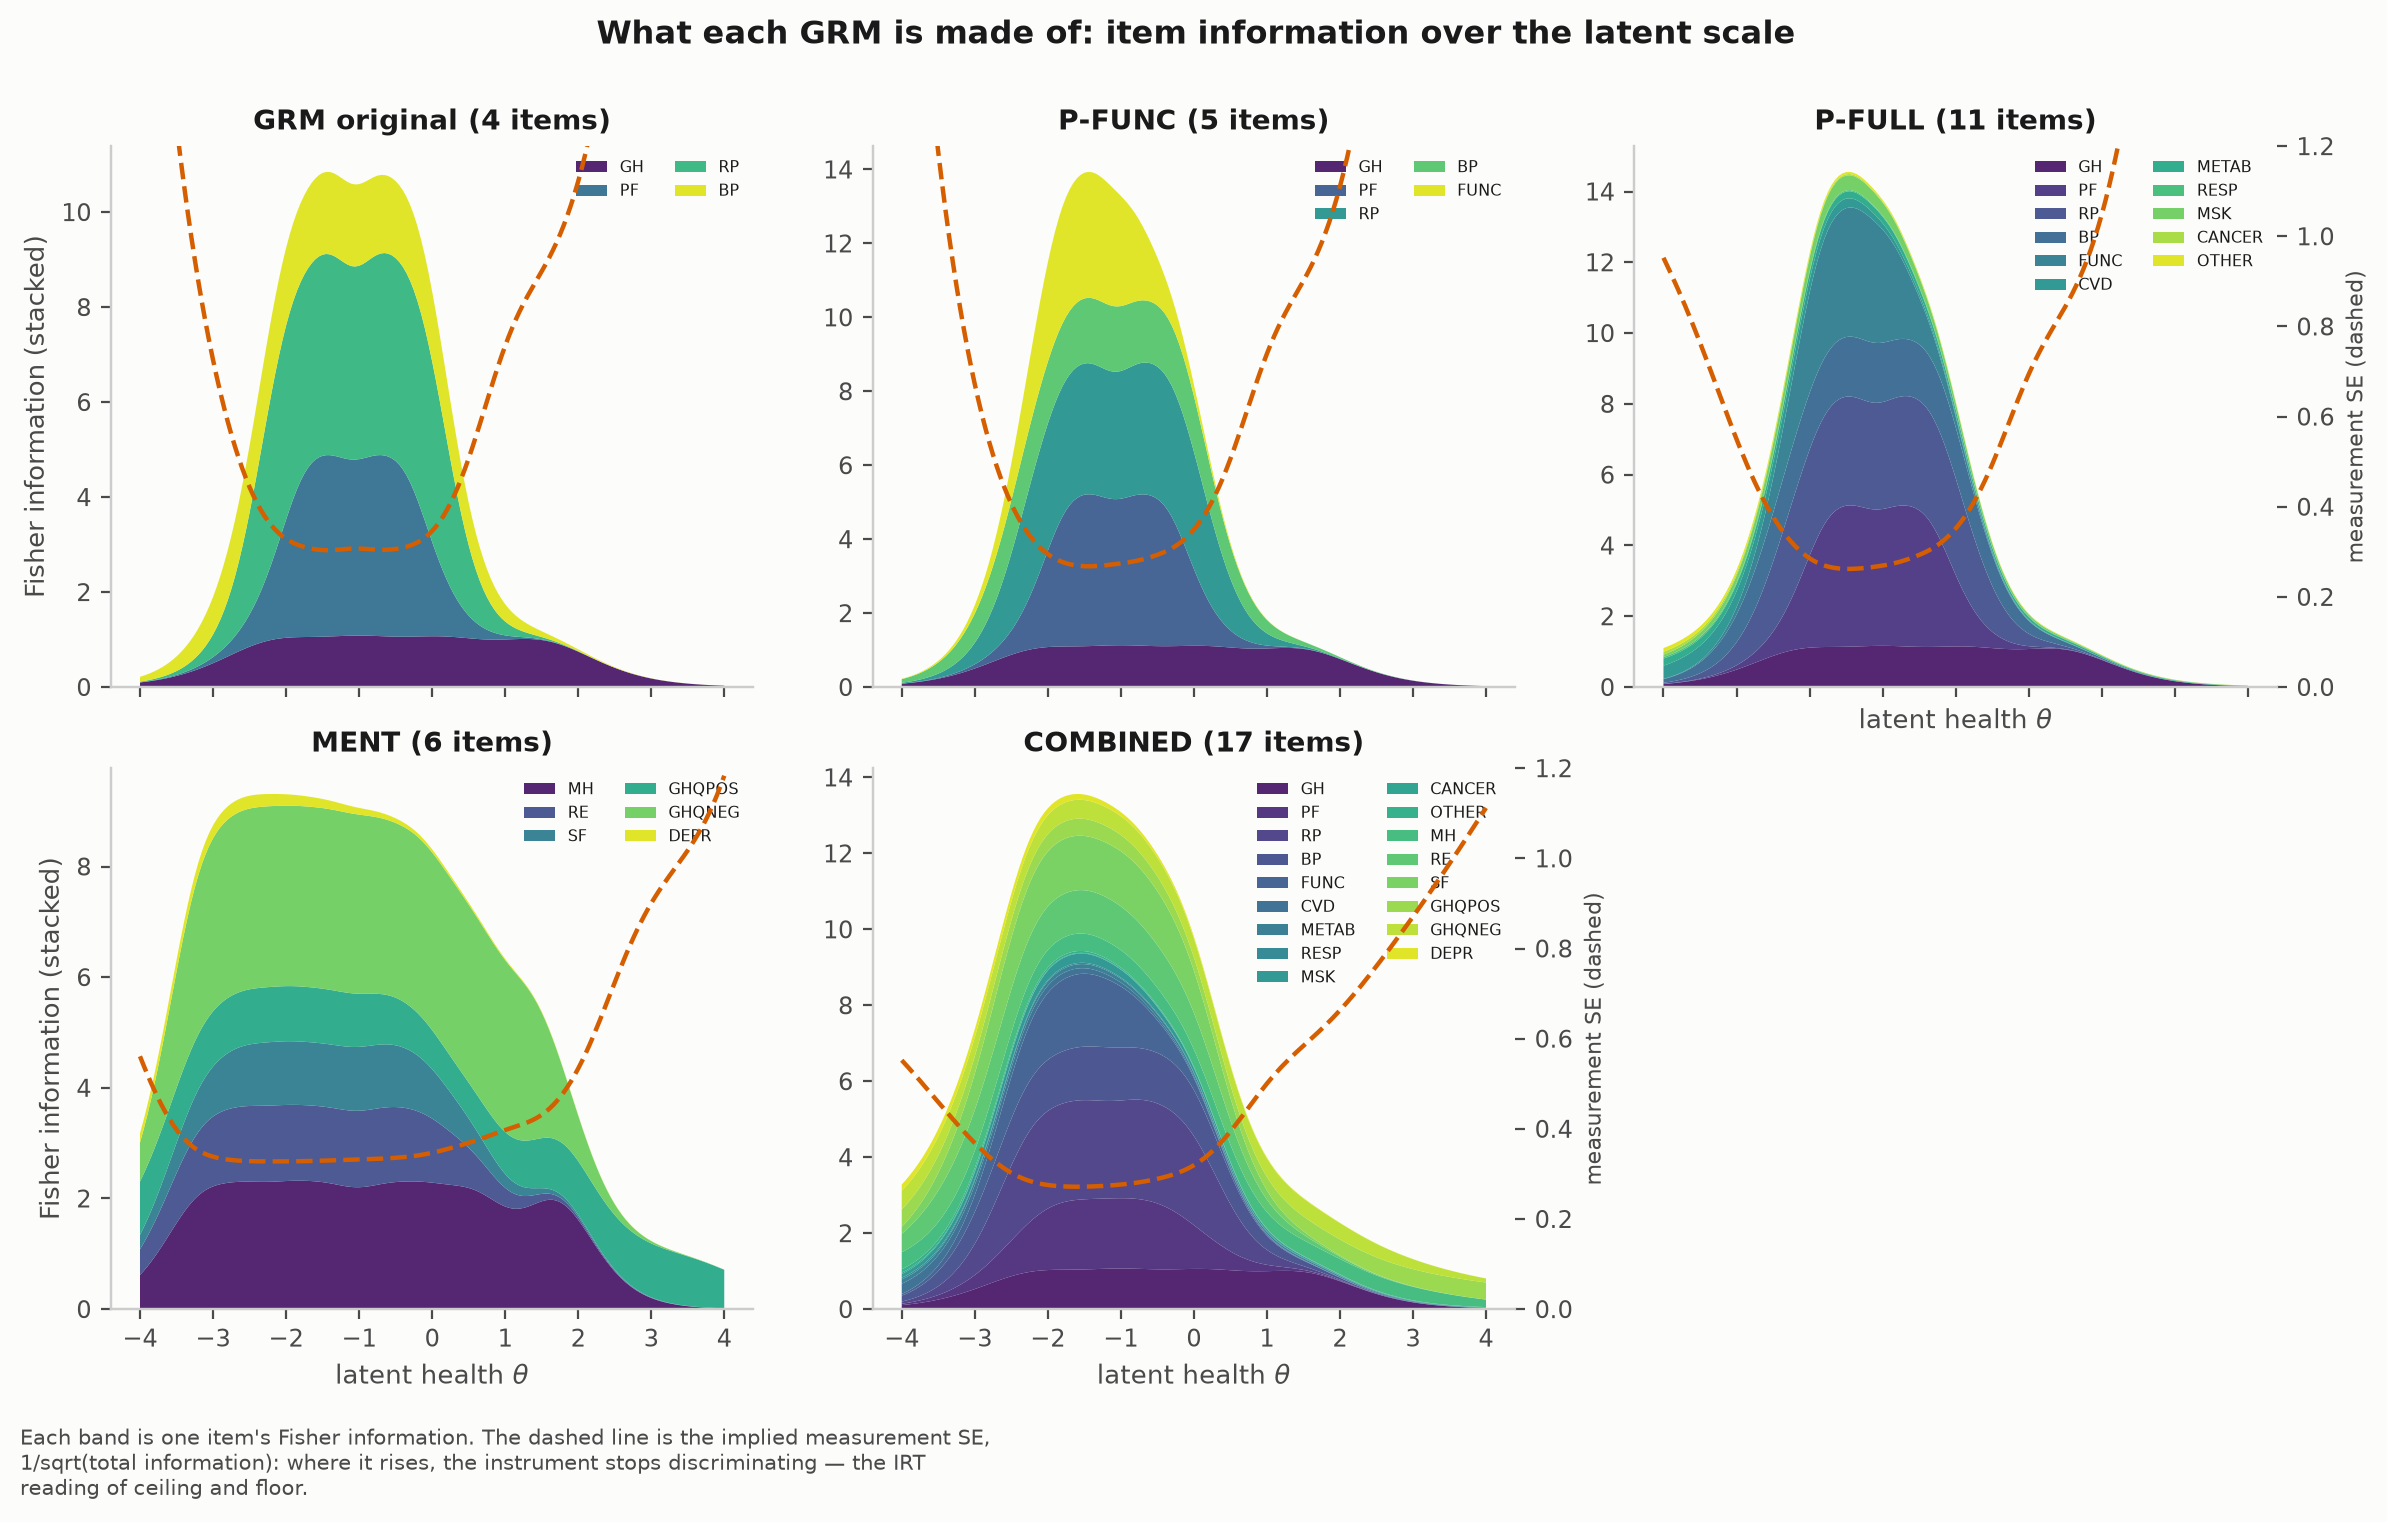
\includegraphics[width=\linewidth]{fig_grm_information}
\caption{What each GRM is made of: stacked item information over the latent
scale, with the implied measurement SE (dashed, right axis); each band is one
item, ordered as in the legend.
%
\emph{Panels:} \textbf{GRM original} is the four-testlet physical measure
replicated from the EIT note; \textbf{P-FUNC} adds the functioning testlet;
\textbf{P-FULL} adds the six diagnosis groups; \textbf{MENT} is the mental
bank; \textbf{COMBINED} is all seventeen items at once.
%
\emph{Physical items, from the SF-12:} \textbf{GH} general health (the single
self-rated-health question), \textbf{PF} physical functioning (moderate
activities, climbing stairs), \textbf{RP} role-physical (cutting down or
being limited at work because of physical health), \textbf{BP} bodily pain;
\textbf{FUNC} is the count of Equality Act physical limitations (mobility,
lifting, dexterity, coordination, personal care).
%
\emph{Diagnosis groups:} \textbf{CVD} cardiovascular events, \textbf{METAB}
diabetes and high blood pressure, \textbf{RESP} chronic airway disease,
\textbf{MSK} arthritis, \textbf{CANCER}, \textbf{OTHER} the pooled remainder
of thyroid, liver and epilepsy (\S\ref{sec:groups}).
%
\emph{Mental items:} \textbf{MH} mental health (calm; downhearted),
\textbf{RE} role-emotional (cutting down or working less carefully because of
emotional health), \textbf{SF} social functioning (health interfering with
social activities), \textbf{GHQPOS} and \textbf{GHQNEG} the positively- and
negatively-worded halves of the GHQ-12, \textbf{DEPR} ever-diagnosed clinical
depression.
%
FUNC adds a broad band of precision on the ill side; the condition items are
visibly thin; GHQ-negative dominates the mental bank; the combined bank is
tallest and widest but its SE still rises sharply above $\theta \approx +1$.}
\label{fig:info}
\end{figure}

\section{How the measures relate}

Correlations over all person-years (\code{descriptives/01}):

\begin{center}\small
\begin{tabular}{lccc}
\toprule
 & $\theta$ phys (FULL) & $\theta$ ment & $\theta$ combined \\
\midrule
original GRM (4 testlets) & \textbf{0.985} & 0.48 & 0.92 \\
UKHLS PCS & 0.904 & 0.23 & 0.76 \\
physical-only composite & 0.946 & 0.48 & 0.90 \\
UKHLS MCS & 0.27 & \textbf{0.882} & 0.58 \\
GHQ-12 Likert & $-0.38$ & $\mathbf{-0.904}$ & $-0.64$ \\
SF-6D utility & 0.71 & \textbf{0.799} & 0.88 \\
chronic count & $-0.58$ & $-0.21$ & $-0.51$ \\
$\theta$ phys $\times$ $\theta$ ment & \multicolumn{3}{c}{\textbf{0.457}} \\
\bottomrule
\end{tabular}
\end{center}

Three reads. The physical GRM is the object the project already validated,
with functioning attached. The mental GRM is the MCS/GHQ construct without
the orthogonality artifact. SF-6D correlates \emph{more} with the mental
theta (0.80) than the physical one (0.71) --- and its closest cousin is the
\emph{combined} bank (0.88): the SF-6D was a mixed measure all along.

\begin{figure}[H]

\includegraphics[width=\linewidth]{fig_moments_grid}
\caption{Mean, variance and the rows of the covariance matrix (the empirics
note's anatomy) for the full metric suite, two banks of six. GHQ and the
chronic count are \emph{negated}, so on every panel higher means better
health. The mental family (MCS, GHQ, mental GRM) shows the textbook late-life
wellbeing improvement; the physical measures share one anatomy ---
accelerating mean decline, rising-then-plateauing dispersion, fanning
covariance rows; the chronic count gives the physical mean and variance reads
from items fully disjoint from the SF-12, while its covariance row carries no
persistence information because the count cannot fall (so its negated series
cannot rise).}
\label{fig:moments}
\end{figure}

Two cautions on the mental hump, because on an auto-scaled axis it looks
dramatic. It is modest in size: mean GHQ falls from $11.75$ at age 55 to
$10.24$ at 70, which on a $0$--$36$ scale with a standard deviation of $5.62$
is $0.27$ sd; the axis spans less than two points, which is what makes it
read as a step change. And \emph{most of it is composition rather than
ageing}: among the 1{,}461 people observed in both windows, mean GHQ improves
by only $0.44$ points between ages 53--57 and 68--72, against a
cross-sectional gap of $1.42$ over the same ages, so under a third of the
apparent improvement survives holding the people fixed. The remainder is
selective non-response and attrition --- GHQ completion falls from $91\%$ at
age 70 to $77\%$ at 90 --- together with cohort differences. This applies to
every panel of the figure: these are pooled cross-sections in which age,
cohort and period are confounded, and they are descriptive scaffolding rather
than within-person trajectories. The mixture models of \S\ref{sec:ar1} do use
within-person information and are not subject to it.

\begin{figure}[H]
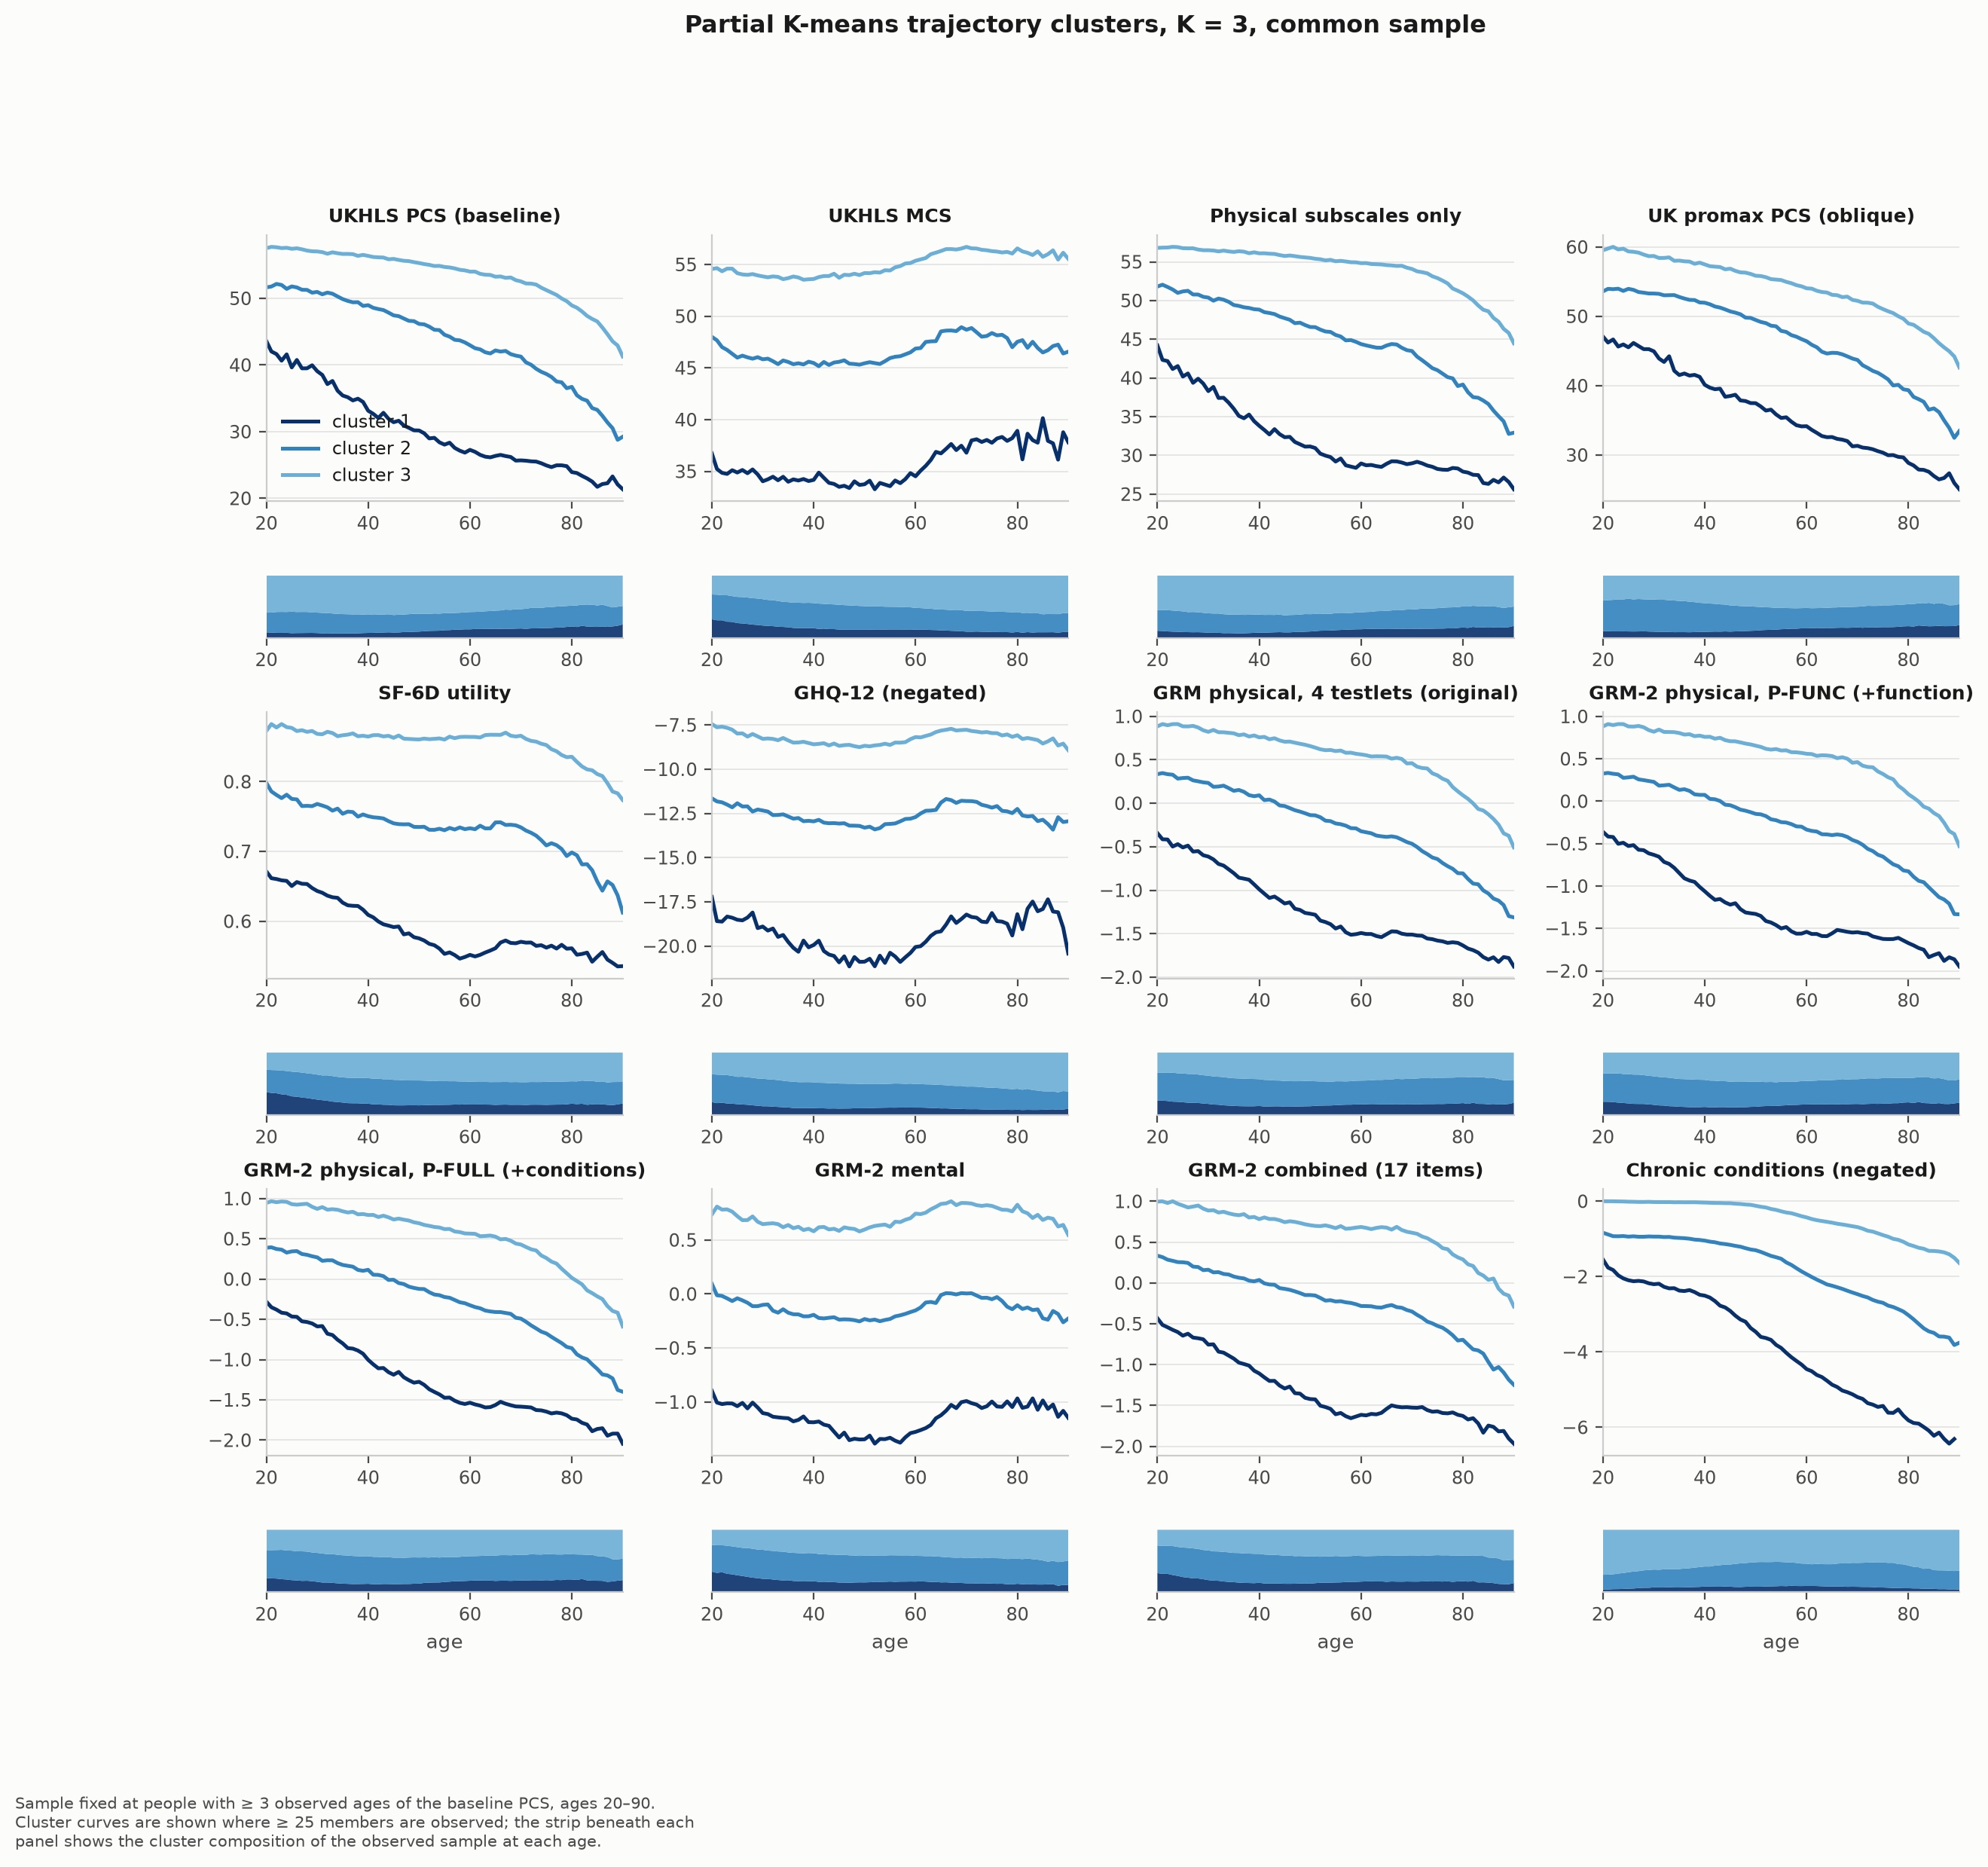
\includegraphics[width=\linewidth]{fig_cluster_trajectories}
\caption{Partial K-means trajectory clusters ($K=3$, 50 seeded inits,
sample fixed at people with $\ge 3$ observed baseline-PCS ages, ages
20--90), across the same twelve measures as Figure~\ref{fig:moments}. GHQ and
the chronic count are negated so every panel runs higher = better health. The
chronic count is monotone by construction, so its three bands can only fall
and never cross --- a property of the measure, not a finding about people.}
\label{fig:clusters}
\end{figure}

Partial K-means (Figure~\ref{fig:clusters}): changing the \emph{scoring}
moves the typology modestly while changing the \emph{construct} redraws it.
Against the PCS baseline, on the common sample:

\begin{center}\small
\begin{tabular}{lrrr}
\toprule
Measure & ARI & \% same cluster & chance \\
\midrule
Physical subscales only & \textbf{0.667} & 87.9 & 43.0 \\
UK promax PCS (oblique) & 0.464 & 79.4 & 39.5 \\
P-FUNC & 0.442 & 76.9 & 38.1 \\
GRM original (4 testlets) & 0.425 & 75.6 & 37.7 \\
P-FULL & 0.409 & 74.9 & 37.5 \\
GRM combined (17 items) & 0.266 & 66.1 & 36.8 \\
SF-6D utility & 0.185 & 60.0 & 37.4 \\
Chronic conditions (negated) & 0.120 & 56.1 & 44.3 \\
GHQ-12 (negated) & 0.079 & 51.4 & 40.8 \\
GRM mental & 0.074 & 49.2 & 37.1 \\
UKHLS MCS & \textbf{0.053} & 48.0 & 40.0 \\
\bottomrule
\end{tabular}
\end{center}

The physical measures agree substantially with the baseline whatever the
scoring --- 0.41 to 0.67 --- and the ordering is instructive: the composite
that merely re-weights the same subscales agrees most, the IRT re-spacings
sit in the middle, and the further a measure moves from the PCS's item set
the lower it falls. The mental measures sit at the bottom, essentially at
chance: MCS at ARI 0.053 and the mental GRM at 0.074, with same-cluster rates
of 48\% and 49\% against chance rates of 40\% and 37\%. The combined bank
lands between the two families at 0.27, which is what a physically-dominated
mixture of them should do. So the physical typology is robust to how physical
health is scored, and the mental dimension partitions people almost
independently of it --- the same conclusion the two-bank correlation of
$0.457$ reaches by a different route.

\section{The ever-diagnosis question, resolved}
\label{sec:ever}

The misgiving: historical diagnoses accumulate mechanically with age, so a
diagnosis-bearing measure could manufacture ``decline'' out of stale
paperwork. Four reads.

\begin{figure}[H]
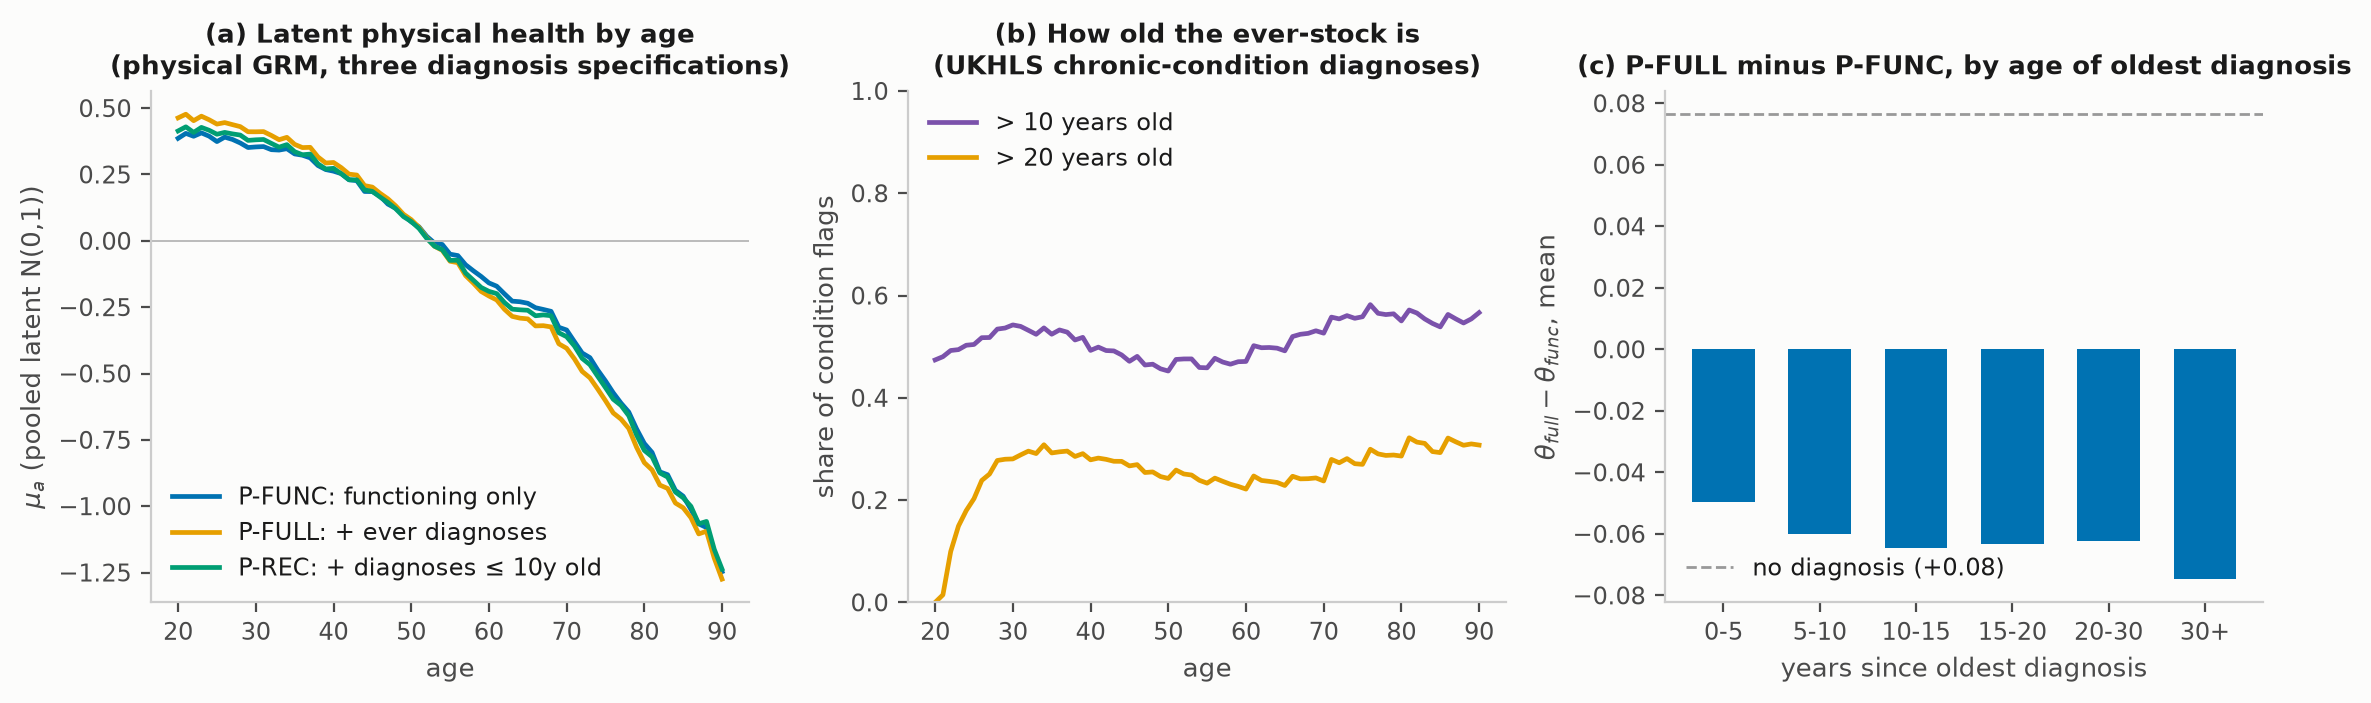
\includegraphics[width=\linewidth]{fig_ever_sensitivity}
\caption{The ever-diagnosis question, all three panels on the physical
GRM. (a) latent age profiles $\mu_a$ under P-FUNC (functioning only), P-FULL
(plus ever-diagnoses) and P-REC (plus diagnoses at most ten years old); (b)
the staleness of the UKHLS chronic-condition stock; (c) the per-person gap
$\theta_{\text{P-FULL}} - \theta_{\text{P-FUNC}}$ against the age of that
person's oldest diagnosis.}
\label{fig:ever}
\end{figure}

\textbf{(1) The aggregate effect is real but bounded.}
$\mu(80)-\mu(30)$ is $-1.117$ SD functioning-only, $-1.247$ with
ever-diagnoses, $-1.170$ with only diagnoses $\le$10 years old. Diagnoses
steepen the measured lifecycle decline by 0.130 SD (12\%), and 59\% of that
extra steepness comes from diagnoses more than a decade old --- leaving the
stale-accumulation component at $\sim$6\% of the total decline.

\textbf{(2) The potential was much larger than the realised effect.} Half
the ever-stock is $>$10 years old at every age past 40 (\S2.4). The damage
stays small because the estimator protects itself: items that cannot predict
the functioning responses get low discriminations, so stale-heavy condition
items simply carry little weight.

\textbf{(3) The items cannot tell stale from fresh --- which cuts both
ways.} The person-level penalty $\theta_{\mathrm{full}} -
\theta_{\mathrm{func}}$ is flat in the age of the oldest diagnosis ($-0.05$
SD at 0--5 years, $-0.075$ at 30+). Read as measurement of \emph{current}
health, that is exactly the mechanism feared: no within-item discounting
exists. It is an argument \emph{against trusting ever-items as current-state
measures}, and simultaneously the reason their damage is capped.

\textbf{(4) Asked directly, the data mostly decline to discount.} P-TIMED
splits every group into recent ($\le$10y) and stale ($>$10y) items and lets
the model estimate their separate discriminations --- the in-framework
analogue of an estimated recency-weight function:

\begin{center}\small
\begin{tabular}{lccc}
\toprule
Group & $a$ recent & $a$ stale & ratio \\
\midrule
CVD & 1.19 & 1.21 & 0.99 \\
METAB & 0.59 & 0.81 & 0.72 \\
RESP & 0.68 & 0.29 & \textbf{2.31} \\
MSK & 0.83 & 1.22 & 0.68 \\
CANCER & 0.59 & 0.56 & 1.05 \\
OTHER & 0.63 & 0.63 & 1.00 \\
\bottomrule
\end{tabular}
\end{center}

Only respiratory disease wants a discount (remitting childhood asthma). For
arthritis and the metabolic conditions the \emph{stale} item is more
informative --- progressive diseases, where an old diagnosis means longer
duration and worse current health. The mechanistic-accumulation story is
really a story about \emph{remitting} conditions; for progressive conditions
the old diagnosis is legitimately informative.

\textbf{Related literature.} Estimating recency weights on past exposures is
the weighted-cumulative-exposure literature (Sylvestre \& Abrahamowicz 2009;
review in Kelly et al.\ 2024; R package \code{WCE}), with spline-estimated
weight-by-recency functions --- P-TIMED is its two-knot IRT analogue.
Letting item parameters vary continuously with a covariate such as time
since diagnosis is moderated nonlinear factor analysis (Bauer \& Hussong
2009; regularised variants for DIF detection), the natural next refinement
if a smooth weighting is ever needed. The simpler administrative-data
practice is a fixed lookback window (Preen et al.\ 2006), which P-REC
implements. Health-state valuation handles the same issue with acute
vs.\ post-acute utilities for events like stroke.

\textbf{Verdict.} For lifecycle \emph{dynamics}, use P-FUNC (or the original
GRM, $r=0.994$): a pure current-state instrument. P-FULL is a sound
descriptive companion whose accumulation bias is now characterised and
bounded ($\sim$0.08--0.13 SD over the lifecycle, concentrated in remitting
conditions); P-REC and P-TIMED are its sensitivity band. Where conditions
matter substantively, model them as separate channels in the Bayesian
mixture, where ``ever'' is the correct state variable.

\section{One dimension or two? The combined GRM}
\label{sec:combined}

The combined bank (all seventeen items, one latent dimension) fits, scores,
and correlates sensibly ($r=0.92$ with the physical bank, 0.75 with the
mental, 0.88 with SF-6D). But it fails the assumption the others satisfy:
after conditioning on its single dimension, the mental items remain strongly
positively correlated --- $Q_3(\mathrm{MH}, \mathrm{GHQ}^-)=+0.58$,
$Q_3(\mathrm{GHQ}^+, \mathrm{GHQ}^-)=+0.54$, $Q_3(\mathrm{MH},
\mathrm{RE})=+0.33$ --- while the physical side stays clean (max
phys--phys $Q_3$ $+0.20$). That residual clustering is the data saying the
mental items share a dimension the combined score cannot represent: with
$r(\theta_P,\theta_M)=0.457$, one dimension is a genuine misspecification,
not a summary. The same criteria table shows the cost in substance: the
combined score reintroduces a mental-health artifact of $-0.82$ SD at a
fixed physical profile (the physical banks: $0.00$), and its cohort spread
collapses to 0.06 SD not because it is clean but because physical health
improving and mental health deteriorating across cohorts \emph{cancel}
inside it --- precisely the mixing the EIT note warned about. Use it only
where a single index is externally imposed; a bifactor model (general +
physical/mental group factors) would be the defensible one-number
construction if that need becomes real.

\begin{figure}[H]
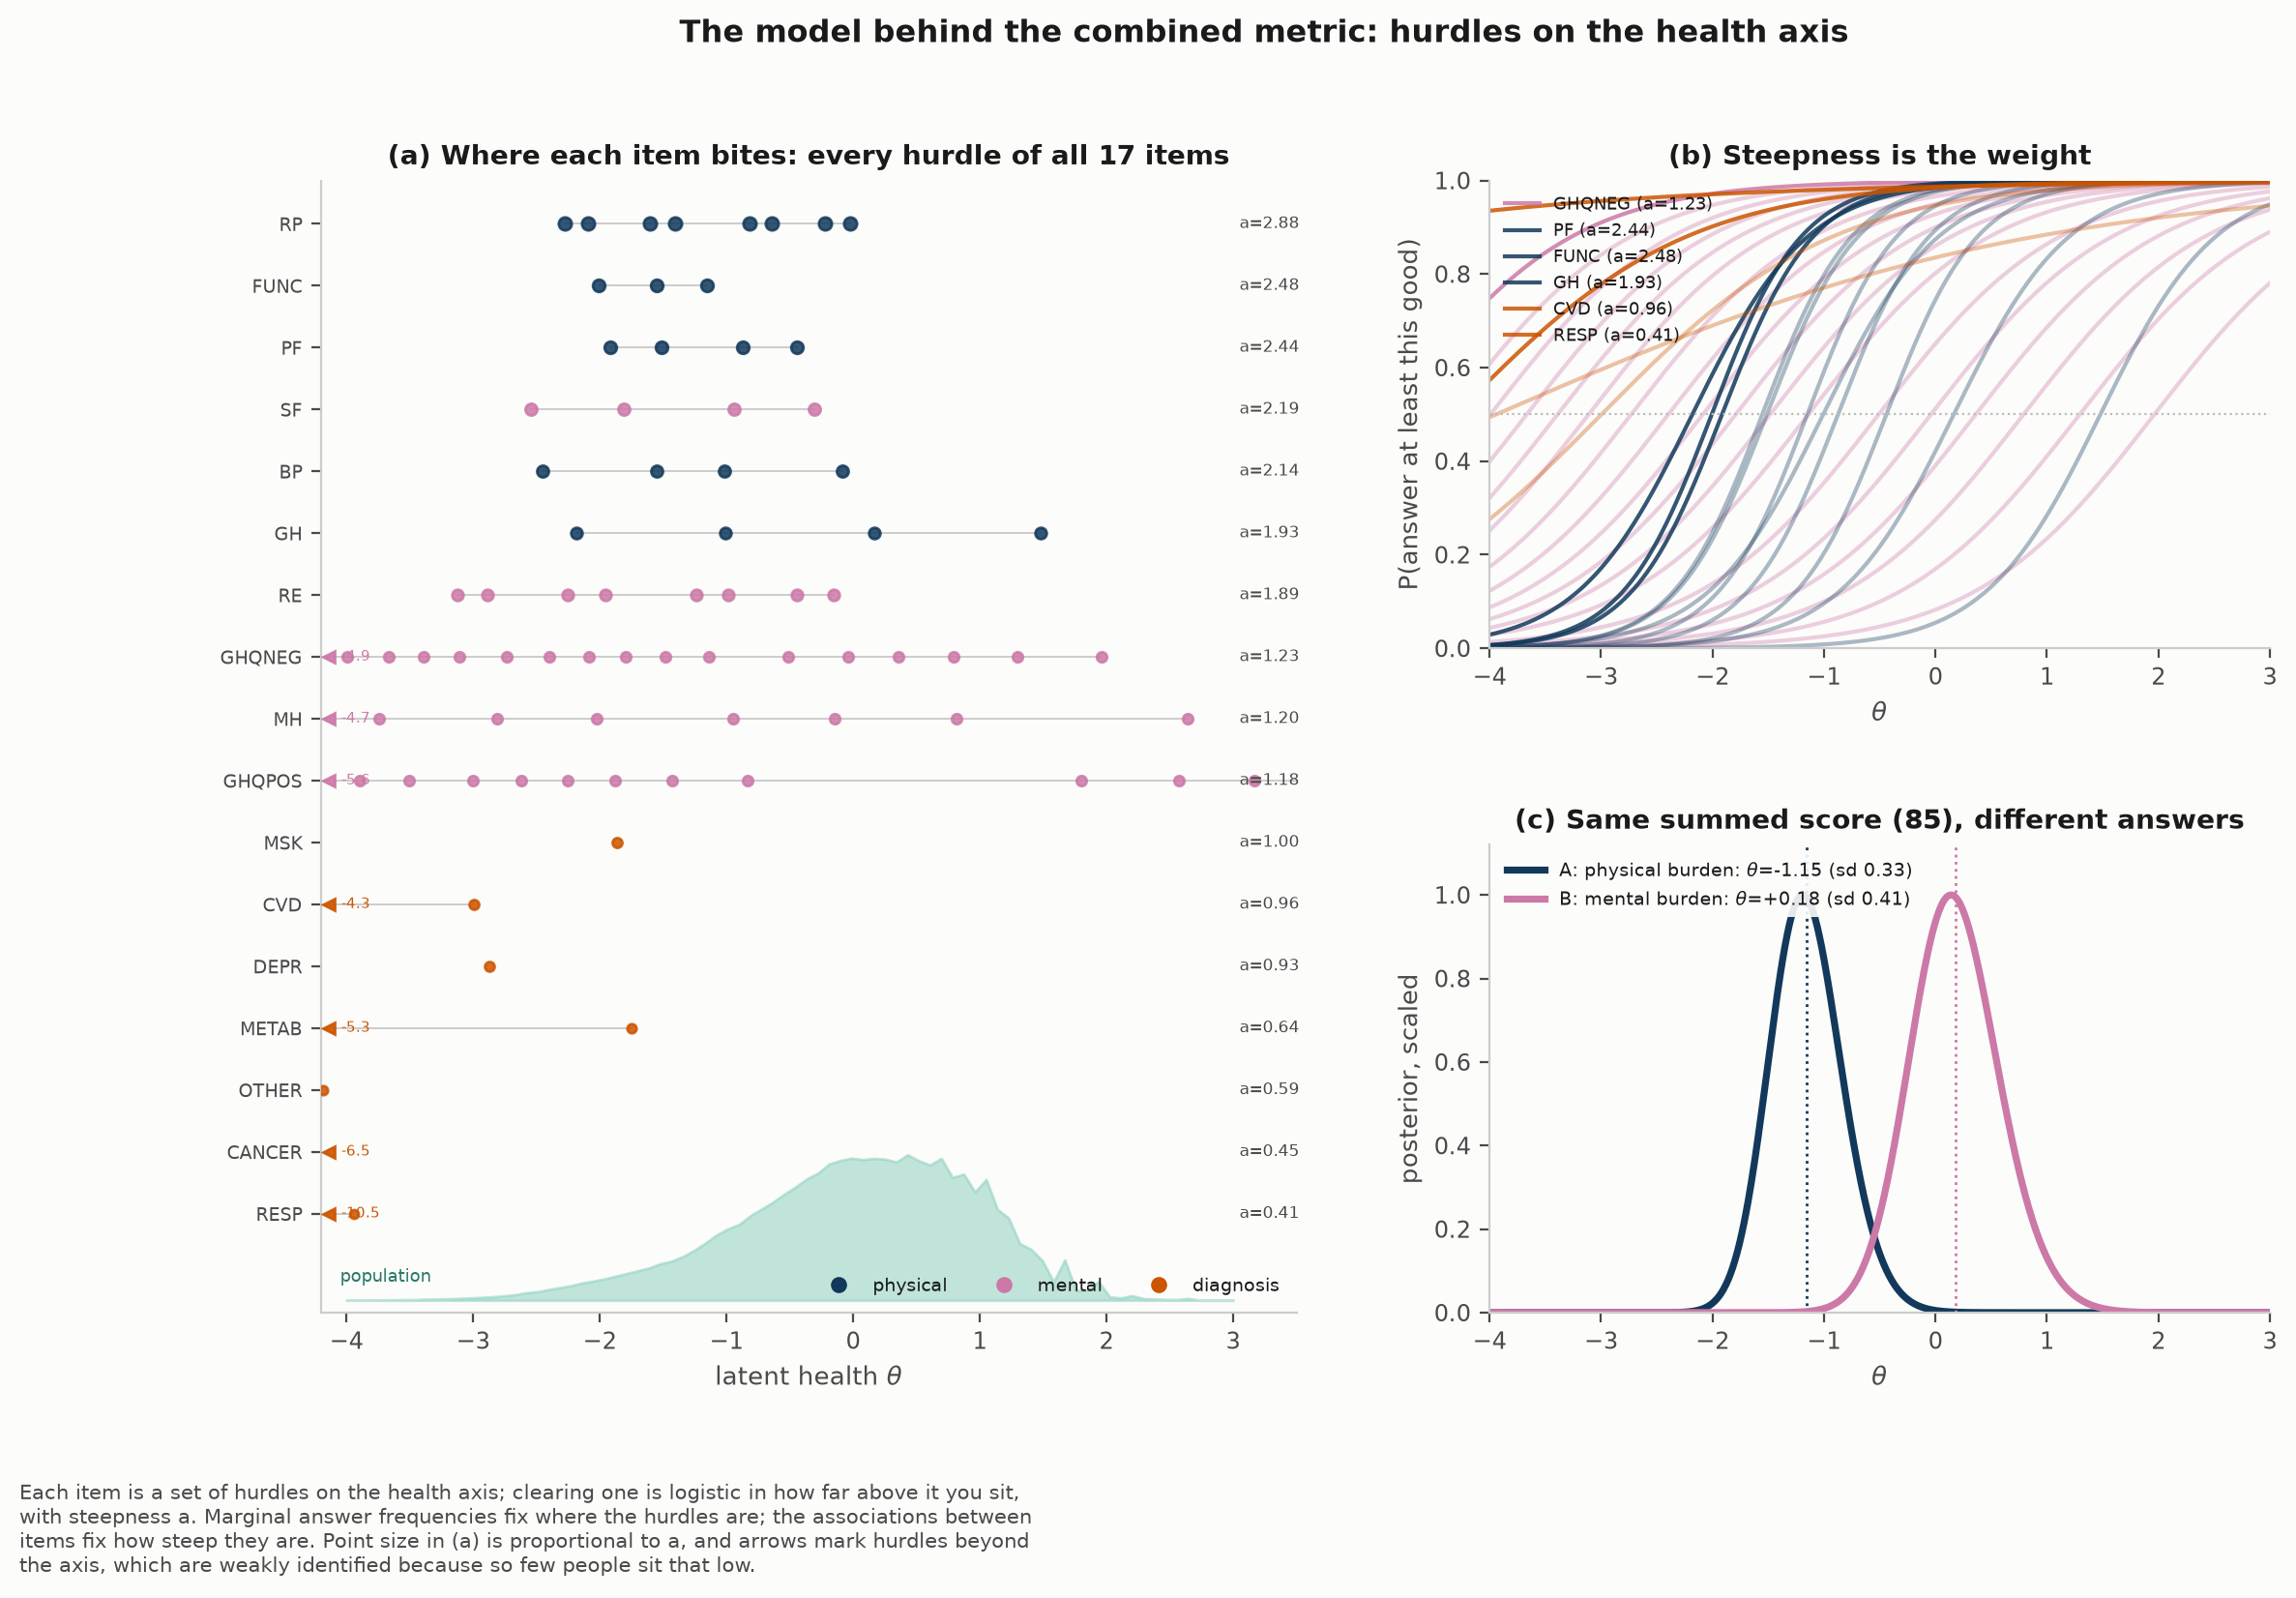
\includegraphics[width=\linewidth]{fig_combined_grm_model}
\caption{The model behind the combined metric, in the empirics note's
hurdles-on-the-health-axis form, for the most all-encompassing bank. (a)
every hurdle of all seventeen items against the population distribution of
$\theta$; (b) the hurdle curves for items spanning the weight range; (c) two
people whose category numbers sum to the same total.}
\label{fig:combmodel}
\end{figure}

Figure~\ref{fig:combmodel} draws the combined bank as a set of hurdles.
Panel (a) makes the division of labour visible: the physical items (RP, FUNC,
PF, BP, GH; $a = 1.9$--$2.9$) cluster their hurdles between $-2.5$ and $0$,
the mental items (GHQNEG, MH, GHQPOS; $a = 1.2$) spread theirs across the
whole axis and beyond it, and the diagnosis items ($a = 0.4$--$1.0$) sit far
to the left. Panel (c) then shows what that means for a score. Two people
whose answers sum to exactly the same total --- one carrying the deficit on
the physical items, the other on the mental ones --- receive
$\theta = -1.15$ and $\theta = +0.18$, a gap of $1.3$ standard deviations.
The combined bank is not a balanced physical--mental index; it is
physically dominated, because the physical items are the steeper and hence
the more reliable ones. That is a second, independent reason (alongside the
residual clustering of \S\ref{sec:combined}) to prefer the two-bank design.

\begin{figure}[H]

\includegraphics[width=\linewidth]{fig_grm_versions}
\caption{The measure-choice panel across measures (the empirics note's
Figure 30, rebuilt): mean age path, dispersion, how much room each measure
has left at its two limits, and the two contamination reads. Seven measures:
UKHLS PCS, SF-6D utility, the original four-testlet GRM, P-FUNC, P-FULL, the
mental GRM and the combined GRM. Panel (c) now carries both limits --- the
solid line is the share of person-years at the measure's exact maximum, the
dashed line, mirrored below zero, the share at its exact minimum, and both
are read as positive percentages. The asymmetry is the point: ceiling mass
runs to $15\%$ at the young end while floor mass never exceeds about $1.5\%$
anywhere, so these instruments run out of room among the healthy long before
they do among the ill.}
\label{fig:versions}
\end{figure}

\section{Ceiling and floor}
\label{sec:ceiling}

Two different questions hide under ``ceiling effects'': how much probability
mass sits at the best attainable response profile, and whether the
instrument can \emph{discriminate} among the healthy. More items help
enormously with the first and only marginally with the second.

\begin{center}\small
\begin{tabular}{lrrrrr}
\toprule
Measure & ceiling \% & floor \% & range (sd units) & psd at top & psd at bottom \\
\midrule
UKHLS PCS (12 items) & 0.89$^{a}$ & $\sim$0 & 6.5 & --- & --- \\
Physical-only composite & 9.95 & 0.91 & 4.1 & --- & --- \\
SF-6D utility & 2.98 & 0.18 & 4.7 & --- & --- \\
GHQ-12 Likert & 0.20 & 0.31 & 6.4 & --- & --- \\
GRM original (4 testlets) & 9.55 & 0.97 & 4.4 & 0.65 & 0.45 \\
P-FUNC & 9.53 & 0.76 & 4.5 & 0.65 & 0.44 \\
P-FULL & 7.16 & 0.00 & 5.3 & 0.64 & 0.56 \\
MENT & 0.11 & 0.03 & 6.5 & 0.60 & 0.45 \\
COMBINED & 0.05 & 0.00 & 7.5 & 0.66 & 0.55 \\
\bottomrule
\end{tabular}

{\scriptsize $^{a}$share at the all-best 12-item profile (the exact-maximum
read is degenerate for a continuous derived score). ``psd'' is the EAP
posterior sd at the all-best / all-worst response pattern.}
\end{center}

The optimistic half of the hypothesis is confirmed: ceiling mass collapses
from 9.5\% (original GRM) to 7.2\% with conditions and to 0.05--0.11\% for
the mental and combined banks, and the floors of P-FULL and COMBINED empty
entirely. Panel (c) of Figure~\ref{fig:versions} shows where it binds: the
young end, where the physical banks still park 12--15\% of person-years at
the maximum.

The pessimistic half is also right, and Figure~\ref{fig:info} shows why: the
posterior sd at the very top is $\sim$0.6--0.66 \emph{for every version} ---
seventeen items buy no more precision among the healthy than four, because
every added item has strongly negative thresholds (all these instruments
measure ill-health). Extra items \emph{spread} the top mass into a finer
ranking (ties broken by GHQ and diagnoses) without adding information where
the healthy live. Genuinely fixing the ceiling requires items with positive
thresholds --- vigorous-functioning items of the PROMIS physical-function
type --- which UKHLS does not carry. For the growth mixtures of
\S\ref{sec:ar1} onwards this matters more than it might seem. They do not see
the ordered item categories; they take each person-wave's EAP score as a
Gaussian observation, so an all-best response pattern enters as a single
value at the maximum, with nothing to indicate that the person's true level
may lie above it. Section~\ref{sec:k4} finds the consequence in the estimated
class structure.

\subsection*{The floor, in depth}

The floor is the mirror image, and here the added items genuinely work ---
their negative thresholds sit exactly where the severely ill live
(\code{descriptives/06}, \code{floor\_depth.csv}):

\begin{center}\small
\begin{tabular}{lccccccc}
\toprule
 & \multicolumn{3}{c}{measurement SE at $\theta=$} & min & \% $<-3$ &
\% at worst & distinct $\theta$ in \\
 & $-4$ & $-3$ & $-2$ & $\theta$ & & pattern & bottom 1\% \\
\midrule
GRM original & 2.15 & 0.73 & 0.33 & $-2.61$ & 0.00 & 0.97 & \textbf{2} \\
P-FUNC & 2.12 & 0.67 & 0.30 & $-2.68$ & 0.00 & 0.76 & 3 \\
P-FULL & \textbf{0.95} & \textbf{0.55} & 0.29 & $-3.38$ & 0.03 & 0.00 & \textbf{575} \\
MENT & 0.56 & 0.34 & 0.33 & $-3.72$ & 0.30 & 0.03 & 1{,}524 \\
COMBINED & \textbf{0.55} & \textbf{0.37} & 0.28 & $-4.43$ & 0.24 & 0.00 & 3{,}708 \\
\bottomrule
\end{tabular}
\end{center}

A note on reading Figure~\ref{fig:info}: P-FULL carries visible information
out to the left edge of the axis where the other physical banks have none.
That is real measurement, not an artefact of where the axis stops. Total test
information at $\theta = -4$ is $1.10$ for P-FULL against $0.22$ for P-FUNC,
and at $\theta = -6$ it is $0.37$ against $0.00$; the axis is not hiding a
cliff, the curve simply keeps declining. The information there comes almost
entirely from the diagnosis items --- CVD ($34\%$ of it), METAB ($18\%$),
OTHER ($10\%$) --- whose hurdles sit at $-3.6$ and $-4.1$, precisely in that
region. It is the opposite of a floor effect: a floor effect is information
\emph{collapsing} at the bottom, which is what the functioning-only banks do.
The caveat is that a few of these thresholds are weakly identified because so
few people sit that low (RESP's first hurdle is estimated at $-10.5$, CANCER's
at $-6.5$ in the combined bank), so the far tail should not be read as
precisely located --- but at $\theta = -4$ the contributing hurdles are all
within the range the data actually cover.

The original GRM (and P-FUNC) have a real floor problem: the instrument goes
dark below $\theta\approx-2.5$ (SE 0.7 at $-3$, 2.1 at $-4$), the scale
simply ends at $-2.6$, and the entire bottom percentile collapses onto two
or three response patterns --- the worst-off are a spike, not a
distribution. The condition items repair precisely this: their thresholds
($-2.6$ to $-4.6$) are the only ones deep in the ill tail, so P-FULL keeps
SE at 0.55 at $\theta=-3$, extends the scale to $-3.4$, empties the
worst-pattern spike entirely, and resolves the bottom percentile into 575
distinct positions. Among the P-FUNC bottom \emph{decile} (37.6k
person-years --- the population a prevention analysis targets), P-FUNC
distinguishes 1{,}252 values, P-FULL 16{,}522, COMBINED essentially one per
person-year. The mental bank has the best floor of all (GHQ thresholds reach
$-3.5$; SE 0.34 at $-3$).

This sharpens the ever-diagnosis trade-off of \S\ref{sec:ever}: the
diagnosis items' cost is a bounded accumulation bias in the age gradient;
their benefit is measurement depth among the severely ill, which
functioning items alone cannot provide because severe limitation saturates
them. For analyses that turn on the worst-health group --- describing the
bottom class, targeting --- P-FULL is the better physical instrument; for
population dynamics, P-FUNC remains the clean choice.

\section{Convexity against healthcare use}
\label{sec:convexity}

Is healthcare use convex in health --- falling steeply among the ill, flat
among the healthy --- and does each metric's cardinalisation carry that
shape? Following the construction-note convexity exercise, each outcome is
regressed on the standardised measure and its square on a common sample
(waves 7--15, all fifteen
measures observed; $n = 209{,}042$ in-patient, $208{,}936$ GP,
$208{,}951$ out-patient), with measures oriented so higher = better: on a
declining relationship, a positive quadratic = convex.

One data correction first, and it runs the other way from the one recorded in
an earlier draft of this note. UKHLS gives \emph{three} tiers of contact, not
two: \code{hl2gp} is ``Visited GP in last 12 months'' and \code{hl2hop} is
``Hosp or clinic out-patient last 12 months'', both banded $0$--$4$ and both
running waves 7--15. An earlier draft asserted the opposite --- that
\code{hl2gp} was the out-patient item and that the mainstage carried no
GP-visit count --- on a faulty dictionary parse that matched an adjacent
variable block. The UKDA labels were re-checked directly in waves g, j and o.
Everything previously reported here as ``out-patient'' was in fact GP visits;
the table below separates the two, and the genuine out-patient column is new.
\code{servuse1} (``service use: your local doctor'', yes/no, five waves) is
kept as a supplementary binary.

\begin{figure}[H]

\includegraphics[width=\linewidth]{fig_convexity}
\caption{Healthcare use across the distribution of each measure, and the
quadratic (convexity) term for in-patient admission. All fifteen measures
are tested (Table above); the seven plotted in the first two panels are
UKHLS PCS, SF-6D utility, the original GRM, P-FUNC, P-FULL, the mental GRM
and the combined GRM, each oriented so higher means better health. The
fourth panel sets each bank's $\theta$ (solid) against its TCC (hatched) for
in-patient stays and GP visits: identical people, identical ranking,
different units. Note that \code{hl2gp} is the GP visit band and
\code{hl2hop} the out-patient band; an earlier draft had these swapped.}
\label{fig:convexity}
\end{figure}

\begin{center}\small
\begin{tabular}{lccccc}
\toprule
 & \multicolumn{3}{c}{quadratic term ($t$)} &
\multicolumn{2}{c}{$P(\text{in-patient})$} \\
\cmidrule(lr){2-4}\cmidrule(lr){5-6}
Measure & in-patient & GP & out-patient & bottom 1\% & top 1\% \\
\midrule
UKHLS PCS & $+.011$ (24) & $+.032$ (18) & $+.032$ (20) & .312 & .042 \\
UKHLS MCS & $+.004$ (8) & $+.038$ (22) & $+.020$ (13) & .128 & .134 \\
Physical-only composite & $+.011$ (22) & $+.002$ (1) & $+.025$ (14) & .331 & .033 \\
SF-6D utility & $+.021$ (40) & $+.119$ (61) & $+.111$ (60) & .289 & .039 \\
GHQ-12 (flipped) & $+.003$ (8) & $+.007$ (5) & $+.004$ (3) & .189 & .059 \\
\midrule
\multicolumn{6}{@{}l}{\emph{each bank on both rulers}} \\
GRM original, $\theta$ & $+.020$ (43) & $+.070$ (42) & $+.081$ (52) & .331 & .033 \\
GRM original, TCC & $+.012$ (23) & $+.003$ (2) & $+.023$ (13) & .331 & .033 \\
\addlinespace
P-FUNC $\theta$ & $+.019$ (42) & $+.069$ (42) & $+.083$ (54) & .322 & .033 \\
P-FUNC, TCC & $+.008$ (17) & $\mathbf{-.017}$ $(-9)$ & $+.007$ (4) & .322 & .033 \\
\addlinespace
P-FULL $\theta$ & $+.020$ (45) & $+.067$ (40) & $+.083$ (54) & \textbf{.349} & \textbf{.033} \\
P-FULL, TCC & $+.009$ (17) & $\mathbf{-.026}$ $(-15)$ & $+.001$ (0) & \textbf{.349} & \textbf{.033} \\
\addlinespace
MENT $\theta$ & $+.008$ (19) & $+.062$ (37) & $+.039$ (25) & .206 & .056 \\
MENT, TCC & $+.004$ (10) & $+.018$ (12) & $+.014$ (9) & .206 & .056 \\
\addlinespace
COMBINED $\theta$ & $+.018$ (44) & $+.072$ (49) & $+.078$ (56) & .331 & .032 \\
COMBINED, TCC & $+.010$ (24) & $+.001$ (0) & $+.023$ (16) & .331 & .032 \\
\bottomrule
\end{tabular}
\end{center}

Every bank now appears on both rulers, and the last two columns are the
control: they are rank statistics, so within a pair they are \emph{identical}
across $\theta$ and TCC to three decimals. Anything that moves between the two
rows of a pair is cardinalisation and nothing else.

Four reads.

\textbf{Utilisation is strongly convex in every latent-scale metric.} The
in-patient rate runs from $\sim$24\% in the worst decile to $\sim$3--4\% in
the best (base rate 8.1\%), with the quadratic terms at $t = 40$--45 for the
GRM thetas. The gradient concentrates exactly where \S\ref{sec:ceiling}'s
floor analysis lives: the region in which measures differ in resolution is
the region that carries the utilisation risk.

\textbf{Cardinalisation, not construct, drives the convexity --- and the
three tiers part company.} Each $\theta$/TCC pair ranks people identically,
so every difference below is units and nothing else.

\emph{In-patient admission is convex on both rulers.} Every TCC row keeps a
$t$ between 10 and 24, roughly half the $\theta$ magnitude. Re-ruling moves
the size of the effect and not the conclusion. This is the tier to trust:
it is also the only one measured as a true count rather than a band.

\emph{GP visits are where the ruler decides the answer.} On $\theta$ every
bank is strongly convex, $t = 37$--49. On the TCC the same banks give $+.003$
$(t=2)$ for the original, $+.001$ $(t=0)$ for COMBINED and $+.018$ $(t=12)$
for MENT --- and turn \emph{concave} for both physical banks, $-.017$ $(t=-9)$
for P-FUNC and $-.026$ $(t=-15)$ for P-FULL. A $t$ of $-15$ is not a null
result; it is a confident statement of the opposite shape.

\emph{Out-patient attendance sits between the two.} On $\theta$ it is the
most convex of the three tiers ($t = 52$--56 for the physical and combined
banks). On the TCC it attenuates hard --- to $+.007$ $(t=4)$ for P-FUNC and
$+.001$ $(t=0)$ for P-FULL --- but it does \emph{not} change sign. So the
outright reversal is specific to GP contact, the tier whose gradient is
shallowest and whose top band saturates soonest; for out-patient care the
honest summary is that re-ruling collapses the curvature to nothing rather
than inverting it.

Convexity is therefore a property of the chosen units, and a ``convex health
effects'' claim means nothing until the scale is fixed. Conversely
\code{grmh} is the natural unit when something close to
linear-in-utilisation spacing is wanted --- the near-zero TCC quadratics are
that property, stated --- and $\theta$ the natural latent-normal unit for the
mixture models.

\textbf{The floor resolution pays off in real outcomes.} P-FULL's bottom
1\% has a 34.9\% admission rate against 32.2\% for P-FUNC and 31.2\% for the
PCS: the diagnosis items isolate a genuinely sicker extreme tail, the
outcome-side counterpart of \S\ref{sec:ceiling}'s 575-fold floor
de-clumping.

\textbf{The supplementary GP binary is uninformative about shape.} The
\code{servuse1} yes/no item adds nothing over the \code{hl2gp} band. At a
77.8\% base rate ($n = 23{,}953$ on its five waves) it saturates: the $\theta$
quadratics are $\approx 0$ for every bank. The TCC rows are uniformly negative
and significantly so ($t = -5$ to $-8$), the same units effect seen in the
banded tiers. Bottom-1\% GP use is
$\sim$97\% against 56--74\% at the top, by measure --- a gradient, but the outcome's
own ceiling swamps any curvature. The banded \code{hl2gp} count is the more
informative of the two; an exact visit count would need linked administrative
data.

\subsection{How much of that convexity is real?}
\label{sec:convexdetail}

The figure above plots utilisation against \emph{percentiles} of each
measure, and the claim of convexity deserves more scrutiny than a percentile
axis can give it. Two separate things inflate it.

\textbf{The horizontal scale.} Percentiles are a rank transform, so equal
horizontal steps are equal shares of people rather than equal amounts of
health. For a roughly normal $\theta$ the bottom decile spans far more of the
health scale than the fifth does, and compressing it to the same width bends
the left-hand end upward. Panels (a) and (b) of
Figure~\ref{fig:convexdetail} show the same relationship on the two axes:
the sharp elbow on the percentile axis becomes a smooth decay on $\theta$.
The binning rule itself turns out not to matter --- equal-count and
equal-width bins trace the same curve --- so this is the axis, not the
aggregation. The formal test in the table above was already run on the
measure's own scale, so only the picture was affected; but the picture is
what carried the claim.

\textbf{The vertical scale, which matters more.} In-patient stays run at
$8.2\%$, and the logistic curve is convex everywhere below one half. A
relationship that is exactly \emph{linear in the log-odds} therefore appears
convex when plotted as a probability. Panel (b) draws a logistic with no
quadratic term at all against the observed decile means: it reproduces the
curvature almost exactly. Panel (c) puts the same data on the log-odds scale,
where it is close to a straight line.

\begin{figure}[H]
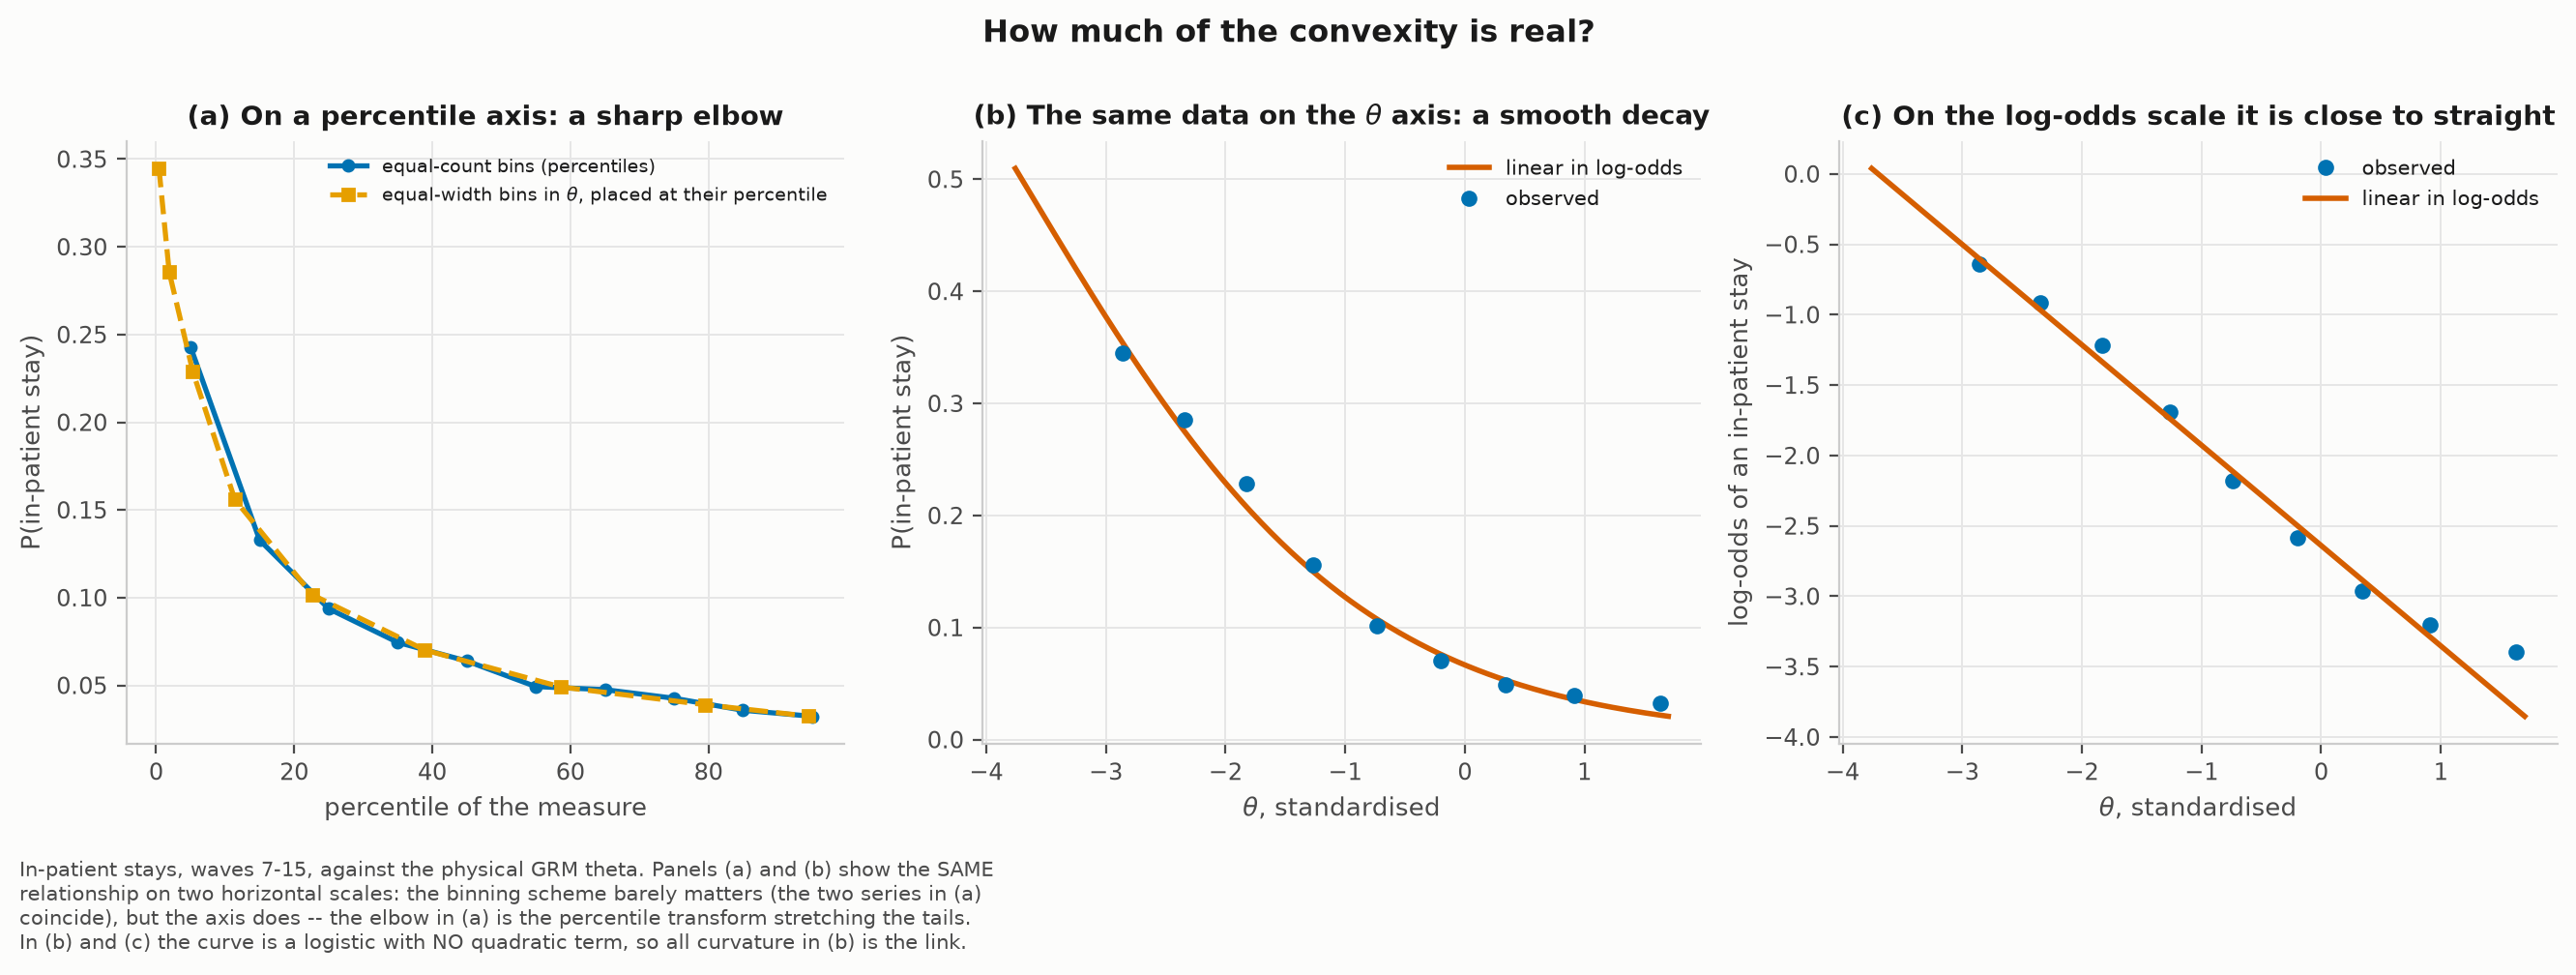
\includegraphics[width=\linewidth]{fig_convexity_detail}
\caption{In-patient stays against the physical GRM $\theta$. The fitted curve
in (b) and (c) is a logistic with no quadratic term, so every departure from
a straight line in (b) comes from the link function alone.}
\label{fig:convexdetail}
\end{figure}

\paragraph{Two axes, not one.} These are separate choices and it is easy to
run them together. Convexity is $\partial^2 y / \partial x^2$, so it depends
on how \emph{both} axes are cardinalised, and the two questions are
independent:

\begin{center}\small
\begin{tabular}{lll}
\toprule
 & what is being chosen & options here \\
\midrule
horizontal & the health measure & $\theta$, \code{grmh}, PCS, SF-6D \\
vertical & the link for the outcome & probability, log-odds \\
\bottomrule
\end{tabular}
\end{center}

The $\theta$ versus \code{grmh} distinction is horizontal: two
cardinalisations of the same latent health. The probability versus log-odds
distinction is vertical: two ways of writing the same risk. In the table
below, differences \emph{down} a column are the horizontal effect and
differences \emph{across} the columns are the vertical one.

The cleanest demonstration that neither is innocuous is the pair $\theta$ and
\code{grmh}. \code{grmh} is the test characteristic curve applied to
$\theta$, a monotone transform, so the two rank every person identically ---
their Spearman correlation is $1.000000$ to six decimal places. They differ
only in spacing, and they differ a great deal: the bottom quarter of the
distribution spans $1.12$ units of $\theta$ but only $0.33$ of \code{grmh},
while the top quarter spans $0.77$ of $\theta$ and just $0.03$ of
\code{grmh}, because the TCC runs into its ceiling. On the log-odds scale
$\theta$ is convex ($+.051$) and \code{grmh} concave ($-.056$).

\emph{Two measures that order people identically disagree about the sign of
the curvature.} Convexity is therefore not a property of the health ordering
at all; it is a joint property of the ordering and the units chosen to
express it. That is the strongest form of the caution for the framework: no
amount of better ranking, more items or finer measurement will settle a
convexity question, because ranking is not what is at issue.

Re-running the quadratic test on both scales makes the point numerically:

\begin{center}\small
\begin{tabular}{lrrrr}
\toprule
 & \multicolumn{2}{c}{probability scale} & \multicolumn{2}{c}{log-odds scale} \\
Measure & $z^2$ coef & $t$ & $z^2$ coef & $t$ \\
\midrule
GRM physical, $\theta$ & $+.020$ & 44.7 & $+.051$ & 8.6 \\
SF-6D utility & $+.021$ & 39.8 & $+.112$ & 18.1 \\
UKHLS PCS & $+.011$ & 23.7 & $\mathbf{-.028}$ & $-4.8$ \\
GRM physical, TCC scale & $+.009$ & 17.4 & $\mathbf{-.056}$ & $-10.2$ \\
\bottomrule
\end{tabular}
\end{center}

\textbf{On the probability scale every measure is emphatically convex; on the
log-odds scale two of the four change sign.} The PCS and the TCC
cardinalisation are mildly \emph{concave} in log-odds. Only $\theta$ and the
SF-6D remain convex there, and $\theta$'s curvature is small against its
linear slope of $-0.71$ per standard deviation.

\textbf{What this means for the framework.} The framework asks whether the
return to preventing a unit of health loss is larger for the already-unwell,
which is a question about the second derivative of a structural relationship
--- and a second derivative is not invariant to how either axis is
cardinalised. Three choices have to be made explicit before the question has
an answer: the health scale ($\theta$, its TCC transform, and the PCS rank
people almost identically but disagree about curvature), the outcome scale
(probability, log-odds, or eventually cost), and, if cost is the target, the
fact that we observe utilisation counts rather than spend at all. The honest
summary of \S\ref{sec:convexity} is therefore narrower than it first
appeared: \emph{utilisation falls steeply with health among the unwell and
flattens among the healthy, and on the natural multiplicative scale for a
risk that relationship is close to log-linear.} A convexity claim strong
enough to carry a policy conclusion needs a cost outcome and a defended
cardinalisation, neither of which UKHLS supplies on its own.

\subsection{If the object is expected cost}
\label{sec:expcost}

The binary outcome is part of the problem but not the whole of it, and
naming which part matters. A binary outcome forces a \emph{bounded} vertical
scale, and on a bounded scale curvature is partly mechanical: below one half
the logistic is convex whatever the data do. That is the vertical half of
\S\ref{sec:convexdetail}. The horizontal half is untouched by it --- $\theta$
and \code{grmh} rank people identically and still disagree about the sign of
the curvature, and no change of outcome fixes that.

But if the motivation is \emph{an individual's expected cost to the health
service}, the vertical problem largely dissolves. Money is a ratio quantity
with a meaningful zero and a meaningful unit, so ``convex in pounds'' is a
substantive claim rather than a convention. Probability and log-odds are two
conventions for writing the same risk and neither is privileged; pounds are
what the system actually spends.

UKHLS carries no spend, but it carries what spend buys: nights as an
in-patient (\code{hospd}) and out-patient attendance bands, waves 7--15. Unit
costs that do not themselves vary with health only rescale the curves, so the
\emph{shape} of expected cost can be studied in physical units without
inventing prices.

\textbf{The decomposition that matters.} Expected nights is
$P(\text{admitted}) \times E[\text{nights} \mid \text{admitted}]$, and
\S\ref{sec:convexity} measured only the first factor. Both move with health:

\begin{center}\small
\begin{tabular}{lrrr}
\toprule
Decile of $\theta$ & $P$(admitted) & nights if admitted & expected nights \\
\midrule
1 (least healthy) & .240 & 13.7 & 3.28 \\
5 & .062 & 4.9 & 0.30 \\
10 (healthiest) & .032 & 3.3 & 0.10 \\
\midrule
bottom vs top & $7.4\times$ & $4.2\times$ & $\mathbf{31.9\times}$ \\
share of the log gap & 58\% & 41\% & --- \\
\bottomrule
\end{tabular}
\end{center}

The least healthy decile is admitted seven times as often \emph{and} stays
four times as long, so it consumes about \textbf{thirty-two times} the bed
days of the healthiest. The intensive margin contributes $41\%$ of the
gradient and was invisible to the binary analysis.

That $31.9\times$ is itself an understatement, because $12.7\%$ of admissions
are childbirth (\code{hospch}), at a mean age of $31.7$ against $57.9$ for
every other admission. Maternity is not health deterioration, and it lands
almost entirely on healthy people in their early thirties, so it inflates the
denominator. Excluding it the ratio is \textbf{$52.7\times$}. Any costing of
these data should separate maternity first.

\begin{figure}[H]
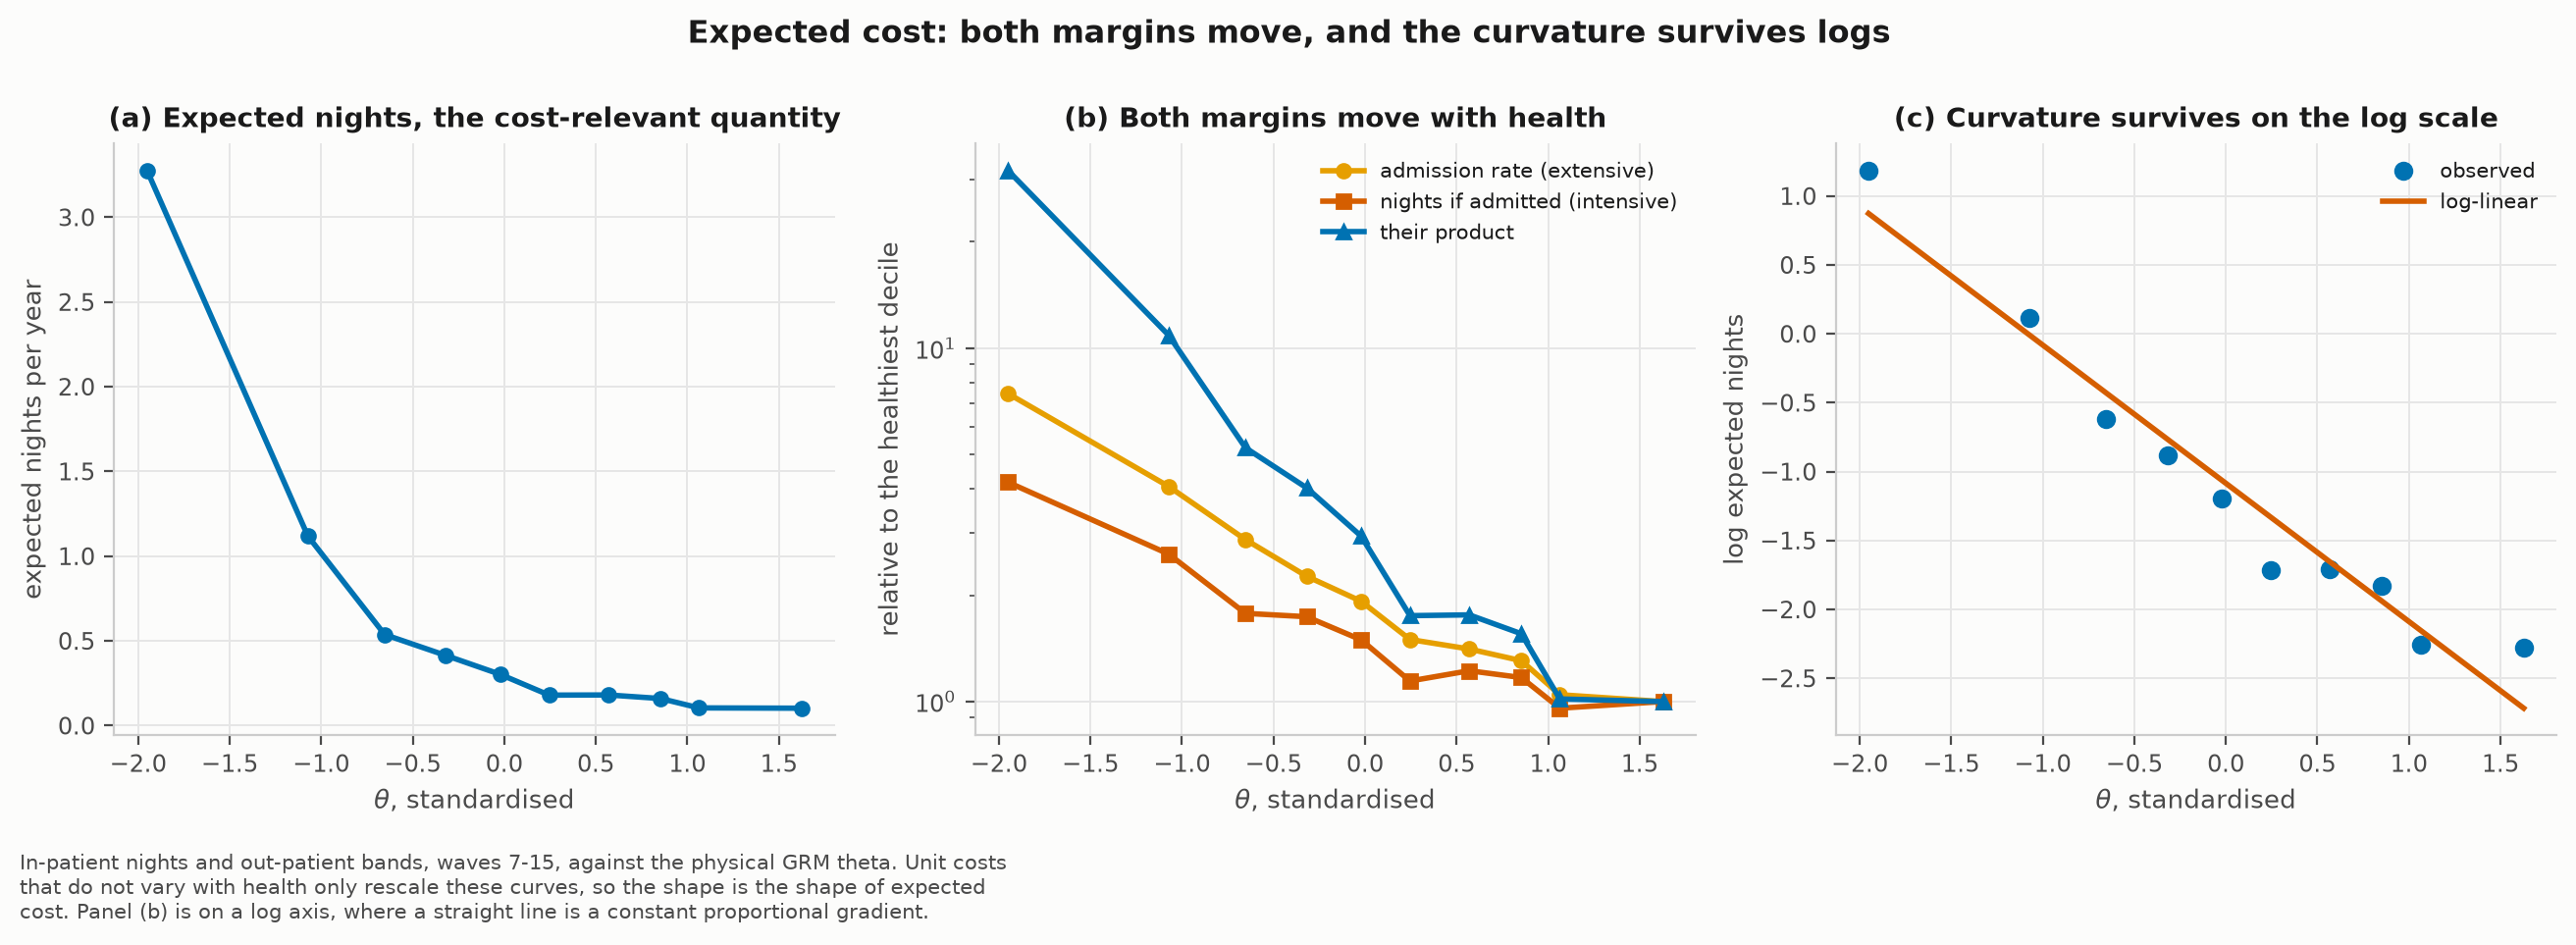
\includegraphics[width=\linewidth]{fig_expected_cost}
\caption{In-patient nights and out-patient bands against the physical GRM
$\theta$. Unit costs that do not vary with health only rescale these curves.}
\label{fig:expcost}
\end{figure}

\textbf{And the curvature survives the log.} On the decile means the
quadratic in $\log E[\text{nights}]$ is $+0.175$, against $+0.087$ for
$\log P(\text{admitted})$ and $+0.016$ for out-patient bands. So where the
binary outcome was close to log-linear --- and flipped sign under other
cardinalisations --- expected bed days is convex \emph{even in logs}, because
the two margins compound. The out-patient channel is log-linear and
contributes none of it; the entire result comes from in-patient nights.

\textbf{So the answer to ``what would make sense'' is threefold.} Use
expected cost, not a binary event: it fixes the vertical axis on a scale that
means something, and it is the quantity the framework is actually about.
Model both margins, because the intensive one carries $41\%$ of the gradient
and a probability model discards it. And define the intervention in units
that survive re-cardinalisation --- a condition prevented, an admission
averted, a year of health --- rather than ``a standard deviation of
$\theta$'', because that is the one problem a better outcome variable cannot
solve. On that footing the framework's convexity assumption looks defensible
in a way \S\ref{sec:convexdetail} alone would not suggest: a factor of
thirty-two, with curvature that survives logging, is a large and robust
gradient.

\textbf{What would still be needed.} Nights are a proxy for cost with fixed
prices per night, which understates the cost of complex admissions and
ignores primary and community care and prescribing entirely. Linked HES cost
data would settle it. And \S\ref{sec:convexlit} applies here too: some of
this gradient is proximity to death rather than health level, which needs
mortality in the model to separate.

\subsection{How far UKHLS can go, and what linkage would add}
\label{sec:utilceiling}

\textbf{There is more in UKHLS than nights.} Beyond \code{hosp} (any
admission) and \code{hospd} (nights), waves 7--15 carry \code{hospch}, a
childbirth flag, and from wave 2 onwards a condition-level breakdown:
\code{hospc}$i$ / \code{hospdc}$i$ record whether an admission and how many
of its nights were due to each \emph{newly reported} condition, and from wave
11 \code{hospcp}$i$ / \code{hospdcp}$i$ do the same for \emph{previously
diagnosed} ones. The condition list runs to about forty codes in the later
waves, well beyond the seventeen of \S\ref{sec:groups} --- COPD, chronic
kidney disease, dementia, the individual cancers and the individual mental
health conditions all appear separately.

\begin{center}\small
\begin{tabular}{llr}
\toprule
Variable & Waves & Coverage \\
\midrule
\code{hosp}, \code{hospd} & 7--15 & all respondents; nights for all admitted \\
\code{hospch} childbirth & 7--15 & $12.7\%$ of admissions \\
\code{hospc}/\code{hospdc} new condition & 2--15 & $21\%$ of admissions \\
\code{hospcp}/\code{hospdcp} prior condition & 11--15 & $11\%$ of admissions \\
\quad either attribution & & $29\%$ of admissions, $65\%$ of nights \\
\code{hl2gp} GP, \code{hl2hop} out-patient & 7--15 & all respondents, banded 0--4 \\
\code{servuse1/2} doctor, hospital & 4, 6, 10, 14, 15 & five waves, binary \\
\bottomrule
\end{tabular}
\end{center}

So the ceiling for UKHLS alone is: expected bed days, with maternity
separable, and with roughly two-thirds of nights attributable to a named
condition. That is enough to weight nights by condition using published
reference costs and to build a considerably better cost proxy than the flat
per-night figure of \S\ref{sec:expcost} --- the attributed nights concentrate
in stroke, COPD, asthma, osteoarthritis, MI and chronic kidney disease, which
have very different unit costs. It is not enough for real costing. Primary
care, prescribing, A\&E attendance, elective versus emergency status and
procedure codes are all absent, and out-patient use is only a four-band
count.

\textbf{Linkage is feasible, with real conditions.} Understanding Society
participates in the UK Longitudinal Linkage Collaboration (UK LLC), which
links consenting participants to NHS primary and secondary care records,
including HES, and holds them in a Trusted Research Environment at Swansea.
Access is free to UK-based researchers for public-good, non-commercial work,
but requires ONS Accredited Researcher status (or enrolment on the Safe
Researcher training), an expression of interest followed by a full
application, and --- the practical constraint for us --- analysis inside the
TRE rather than locally. Nothing in the current pipeline could be run on a
laptop any more.

The binding question is sample size. Linkage covers only consenting
participants: the COVID-19 study contributed roughly $8{,}000$, against the
$84{,}679$ people in our P-FUNC sample, and Understanding Society has stated
an intention to extend linkage to all main-survey participants --- worth
checking the current position before planning around either figure. At
$8{,}000$ the latent-variable machinery in this note would be badly
underpowered; at full coverage it would be transformative, since HES supplies
exactly what is missing: every admission with its diagnosis and procedure
codes, elective versus emergency, and a route to HRG-based costs rather than
proxies.

\textbf{The sensible order.} Exhaust UKHLS first --- separate maternity,
weight the attributable two-thirds of nights by condition, and see whether
the $52.7\times$ gradient and the log-scale curvature survive a better cost
proxy. That is a few days' work on data already on disk, and it would tell us
whether linkage is worth the overhead. If it is, the linkage application is a
months-long process whose main risk is the consented sample being too small
for this kind of model. The staged plan for that work, with the unit-cost
sources and the validation targets, is in \code{cost\_proxy\_plan.pdf}.

\subsection{What the literature actually establishes}
\label{sec:convexlit}

Convexity of healthcare costs in health is widely assumed in prevention
arguments, so it is worth separating what is \emph{accepted}, what is
\emph{measured}, and what is actually \emph{known} about the functional form.
The three come apart.

\textbf{Firmly measured, and about the distribution rather than the shape.}
Spending is extremely concentrated: the top decile of spenders accounts for
more than half of total expenditure, and about a third of them are still in
the top decile a year later. This is robust and uncontroversial, but it is a
fact about the \emph{marginal distribution of spending}, not about the
derivative of cost with respect to health. A concentrated outcome is
consistent with many shapes, including a linear one applied to a skewed
health distribution.

\textbf{Firmly measured, and genuinely about shape --- but on the count
scale.} The multimorbidity literature reports a ``near-exponential''
relationship between the number of chronic conditions and cost, with
expenditure roughly doubling per additional condition and specific
combinations costing more than the sum of their parts (superadditivity).
Here the scale is defensible in a way ours is not: ``one more condition'' has
a meaning that ``one more standard deviation of $\theta$'' does not. But note
what the finding \emph{is}: exponential in the count is exactly linear in log
cost. The headline result of that literature is a multiplicative model, which
is the same shape \S\ref{sec:convexdetail} found in our data --- not evidence
of curvature beyond multiplicative.

\textbf{Assumed by the standard specification, and therefore weakly tested.}
The default model for healthcare costs in health economics is a GLM with a
log link (Manning \& Mullahy 2001; Jones 2010), under which covariates act
multiplicatively by construction. A log-link model is convex in levels
automatically, whatever the data say. So a large share of the empirical
literature cannot be evidence \emph{for} convexity in levels, because it
imposes it; the interesting question --- is there curvature on the log scale?
--- is rarely posed. We found none of the reviewed work testing convexity
against a continuous health measure as a functional-form question.

\textbf{A rival explanation for the shape.} The ``red herring'' literature
(Zweifel, Felder \& Meiers 1999, and the twenty-year reappraisals) argues
that costs track \emph{proximity to death} rather than age or health level,
with spending tripling in the final quarters of life. If most of the
steepness at the bottom of the health distribution is people close to death,
then the apparent convexity in health is partly a survival gradient wearing a
health costume --- which this analysis does not separate. The cost gradient
is estimated without reference to survival, and the mortality channel later
added to the multidimensional model (\S\ref{sec:multimort}) describes hazard
by class, not proximity to death within the cost data.

\textbf{And a caution about the policy inference.} Even granting convexity,
Rose's prevention paradox (1981, 1985) blocks the automatic move from ``the
return per person is highest at the bottom'' to ``target the bottom'': most
cases arise from the large moderate-risk middle rather than the small extreme
tail, so aggregate returns can favour population-wide action even when
individual returns are convex. Convexity in the individual return function
and optimality of targeting are different claims.

\textbf{Where this leaves us.} The proposition that costs rise steeply as
health deteriorates is well measured and not in doubt. The stronger
proposition the framework needs --- that the second derivative is positive on
a defended scale, so that a unit of prevention is worth more to the already
unwell --- is much less established than its ubiquity suggests: it is usually
assumed through a log link, demonstrated on a count scale where it amounts to
log-linearity, or inferred from concentration statistics that do not identify
a shape. Our own finding of near-log-linearity
(\S\ref{sec:convexdetail}) sits comfortably within the literature rather than
against it. Testing the framework's version of the claim needs a cost outcome
rather than utilisation counts, a health scale defended on grounds other than
convenience, and mortality in the model so that proximity to death is not
doing the work.

\section{Latent-class trajectories under AR(1) persistence}
\label{sec:ar1}

The measures feed the Bayesian clustering layer: $K=3$ quadratic growth
mixtures (the consolidated Stan model, partition inits with jitter, 4 chains
$\times$ 1000+1000) on each channel's frozen lifecycle contract, in four
specifications --- no AR term; AR(1) persistence in the class residual; AR(1)
with \emph{within-person holdout}, where each person's last two observations
are excluded from the likelihood and scored as a conditional predictive
density, with the sample restricted to people observed at least five times;
and a state-space specification in which an AR(1) latent health state carries
the persistence and each observation adds an independent one-period
\emph{measurement error} on top (\emph{Separating persistence from
measurement error}, below). Class 1 is worst health
throughout (the anchor convention). All fifteen fits converged. The first
batch of eight took 15.9 h, the three state-space fits 14.9 h, and their three
holdout twins together with the instrument control 17.0 h, each on two
workers.

\begin{center}\footnotesize\setlength{\tabcolsep}{4pt}
\begin{tabular}{llrlllr}
\toprule
Channel & Spec & Persons & $\theta$ (shares) & $\rho$ (persistence) &
max $\hat R$ & wall \\
\midrule
PCS & AR(1) & 50{,}194 & .165 / .273 / .561 & .67 / .31 / .29 & 1.004 & 8.3 h \\
PCS & AR(1) + holdout & 39{,}349 & .146 / .234 / .620 & .67 / .26 / .30 & 1.006 & 6.2 h \\
GRM phys (P-FULL) & baseline & 38{,}963 & .159 / .437 / .404 & --- & 1.003 & 2.0 h \\
GRM phys (P-FULL) & AR(1) & 38{,}963 & .328 / .360 / .312 & .78 / .27 / .39 & 1.001 & 4.1 h \\
GRM phys (P-FULL) & AR(1) + holdout & 29{,}901 & .313 / .362 / .325 & .78 / .26 / .37 & 1.002 & 2.5 h \\
GRM combined & baseline & 38{,}181 & .163 / .454 / .383 & --- & 1.002 & 1.9 h \\
GRM combined & AR(1) & 38{,}181 & .290 / .379 / .331 & .77 / .34 / .44 & 1.002 & 3.6 h \\
GRM combined & AR(1) + holdout & 29{,}280 & .271 / .377 / .352 & .77 / .32 / .44 & 1.003 & 3.1 h \\
\addlinespace
GRM original & ME & 50{,}042 & .267 / .497 / .236 & .95 / .89 / .81 & 1.005 & 11.1 h \\
GRM original & ME + holdout & 38{,}971 & .248 / .498 / .254 & .95 / .89 / .80 & 1.002 & 10.3 h \\
GRM phys (P-FUNC) & ME & 50{,}001 & .254 / .487 / .259 & .95 / .89 / .82 & 1.004 & 9.9 h \\
GRM phys (P-FUNC) & ME + holdout & 38{,}923 & .243 / .487 / .270 & .95 / .89 / .81 & 1.007 & 10.5 h \\
GRM phys (P-FUNC) & ME, P-FULL roster & 38{,}963 & .261 / .489 / .250 & .95 / .89 / .82 & 1.002 & 6.7 h \\
GRM phys (P-FULL) & ME & 38{,}963 & .261 / .478 / .261 & .95 / .90 / .86 & 1.002 & 5.0 h \\
GRM phys (P-FULL) & ME + holdout & 29{,}901 & .249 / .480 / .271 & .96 / .90 / .86 & 1.008 & 6.1 h \\
\bottomrule
\end{tabular}

{\scriptsize ME: AR(1) latent state plus one-period measurement error, with or without holdout. ``P-FULL roster'' is the instrument control: P-FUNC fitted
to the exact person-age cells of the P-FULL contract.}
\end{center}

\textbf{Persistence is strongly class-graded, on every channel.} The
worst-health class carries $\rho_1 = 0.67$--$0.78$ against $0.26$--$0.44$
for the other two, with posterior standard deviations of $0.003$--$0.007$:
shocks to the least healthy class decay several times more slowly than
shocks elsewhere, and the ordering is identical across three different
instruments. This is the mixture-model counterpart of the EIT note's
persistent-layer anatomy, estimated jointly with the class structure rather
than imposed. It is also, as the state-space subsection below shows, a statement about an
\emph{attenuated} parameter: once a one-period measurement error is allowed,
the ordering survives but the grading largely does not, and every $\rho$ here
should be read with that section in view.

\textbf{The AR term, not the scale, redistributes the classes.} The interim
reading of these fits was that the GRM channels produce near-even class
shares where the PCS stays bottom-heavy. The baselines refute the
measurement-scale half of that: without an AR term, \emph{both} GRM channels
put only 16\% in the worst class (.159 and .163), close to the PCS
convention. Adding persistence roughly doubles that share to .29--.33. The
mechanism is visible in the intercepts: the baseline worst class sits at
$\alpha_1 \approx -1.6$ on all three channels, while under AR(1) the GRM
worst class moves up to $\alpha_1 \approx -1.0$ and takes in many more
people. Without persistence, a small extreme class must absorb the
autocorrelation of repeated low observations; once $\rho$ can do that work,
the class boundary moves and a broader, less extreme worst class emerges.
The PCS resists this ($\theta_1$ .165 under AR(1)), which is consistent with
its coarser floor (\S\ref{sec:ceiling}): it cannot separate the severely ill
finely enough for the boundary to move.

\subsection*{Class trajectories and shares}

\begin{figure}[H]

\includegraphics[width=\linewidth]{fig_trajectory_comparison}
\caption{Fitted class mean trajectories $\alpha_k + \beta_k a + \gamma_k
a^2$ (with $a = (\text{age}-55)/10$) for all eleven fits, on each channel's
standardised scale. Channels: the UKHLS PCS, the physical GRM in its P-FULL
specification (\code{theta\_phys\_full}: functioning plus diagnosis groups),
the combined seventeen-item GRM (\code{theta\_combined}), the original GRM
(\code{grm\_theta}) and the functioning-only physical GRM
(\code{theta\_phys\_func}). Line width is proportional to the class share.
``ME'' in the last three titles marks the state-space specification described
below: an AR(1) latent state plus an independent one-period
measurement error. The strip beneath each panel is the class composition of
the person-waves observed at each age.}
\label{fig:trajectories}
\end{figure}

Figure~\ref{fig:trajectories} puts every fit on one standardised axis. Three
regularities hold everywhere: the three classes are ordered in level at
every age and never cross; all three decline; and the worst class declines
\emph{fastest}, so the classes fan apart over the life course. The gap
between the best and worst class widens from $0.9$--$1.9$ sd at age 30 to
$1.8$--$2.2$ sd at age 80, with the narrowest age-30 gaps and the widest
fanning in the three state-space fits.

\begin{center}\small
\begin{tabular}{lrrrrr}
\toprule
Fit & worst-class & \multicolumn{2}{c}{level gap (best $-$ worst)} &
\multicolumn{2}{c}{decline, age 30--80} \\
 & share & age 30 & age 80 & worst & best \\
\midrule
PCS, AR(1) & .165 & 1.24 & 2.20 & $-1.62$ & $-0.66$ \\
PCS, AR(1) + holdout & .146 & 1.35 & 2.19 & $-1.45$ & $-0.61$ \\
GRM phys, baseline & .159 & 1.74 & 2.06 & $-1.22$ & $-0.89$ \\
GRM phys, AR(1) & .328 & 1.21 & 1.81 & $-1.44$ & $-0.84$ \\
GRM phys, AR(1) + holdout & .313 & 1.22 & 1.79 & $-1.32$ & $-0.75$ \\
GRM comb, baseline & .163 & 1.86 & 2.19 & $-0.90$ & $-0.57$ \\
GRM comb, AR(1) & .290 & 1.38 & 1.95 & $-1.12$ & $-0.56$ \\
GRM comb, AR(1) + holdout & .271 & 1.41 & 1.91 & $-0.96$ & $-0.46$ \\
\addlinespace
GRM original, AR(1) + meas. err. & .267 & 0.98 & 1.92 & $-1.47$ & $-0.53$ \\
GRM phys P-FUNC, AR(1) + meas. err. & .254 & 0.97 & 1.94 & $-1.52$ & $-0.55$ \\
GRM phys P-FULL, AR(1) + meas. err. & .261 & \textbf{0.91} & 1.90 & $\mathbf{-1.69}$ & $-0.70$ \\
\bottomrule
\end{tabular}

{\scriptsize Standardised channel units. Class 1 is worst health.}
\end{center}

The specifications differ in \emph{how} they separate the classes, and the
difference is systematic. Adding the AR term to a GRM channel moves the
worst class up in level (its age-30 gap to the best class narrows from 1.74
to 1.21 on the physical channel) while making it decline more steeply
($-1.22 \to -1.44$) and roughly doubling its membership. In other words the
baseline finds a \emph{small, extreme, comparatively flat} worst class; with
persistence available the model instead finds a \emph{larger, less extreme,
faster-declining} one. The ratio of worst-class to best-class decline --- a
compact summary of how much of the story is trajectory divergence rather
than fixed level differences --- rises from $1.37$ to $1.72$ (physical) and
$1.57$ to $2.00$ (combined) when persistence is added, while the PCS sits
at $2.4$--$2.5$ in both its specifications.

The holdout fits track their full-sample siblings closely on every one of
these quantities (shares within $.02$, level gaps within $.11$ sd, declines
within $.18$ sd), so the restriction to people with five or more
observations changes the estimated typology very little.

\subsection*{Separating persistence from measurement error}
\label{sec:meas}

Under the AR(1) specification the observation \emph{is} the state, so $\rho$
has to absorb both genuine persistence and any transient noise in the
instrument. If a GRM score wobbles year to year for reasons that have nothing
to do with health --- a different interviewer, a bad week, the coarseness of a
five-point item --- that wobble enters as a fast-decaying shock and drags
$\rho$ towards zero. The state-space specification separates them: a latent
health state follows the AR(1), and each observation adds independent noise
that does not persist. In reduced form this is ARMA(1,1). Identification comes
from the autocorrelation function, since $\text{corr}(k) = \rho^k \times
\text{signal share}$ for $k \ge 1$, so $\rho$ is fixed by the \emph{ratio} of
successive autocorrelations and the signal share by their \emph{level}. The
state is marginalised by a Kalman filter rather than sampled, so no latent
series enters the parameter vector. Measurement error is one scale per
channel, shared across classes: it is a property of the instrument, not of the
person's class.

\textbf{The specification was validated on simulated data first.} On 1,500
simulated people with $\rho = 0.75$, $\sigma_{\text{state}} = 0.45$ and
$\sigma_{\text{meas}} = 0.35$, the state-space fit recovers $\rho = 0.738$,
$\sigma_{\text{state}} = 0.384$ and $\sigma_{\text{meas}} = 0.280$ against
truths of $0.750$, $0.375$ and $0.292$ on the standardised scale. Fitting
AR(1) to the \emph{same} simulated panel returns $\rho = 0.564$, an
attenuation of $24.7\%$, and inflates $\sigma$ from $0.375$ to $0.505$. The
misspecification the model exists to fix is visible in the recovery exercise
before it is asserted of the data.

\textbf{In the real data the attenuation is far larger than that.} Comparing
P-FULL under the two specifications on the \emph{identical} sample --- the
same 38,963 people and 334,194 person-waves, one specification change:

\begin{center}\small
\begin{tabular}{lrrrr}
\toprule
 & \multicolumn{3}{c}{$\rho$ by class} & \\
Specification & 1 & 2 & 3 & $\sigma$ \\
\midrule
AR(1) & .780 & .274 & .390 & .532 \\
AR(1) + measurement error & \textbf{.954} & \textbf{.902} & \textbf{.862} &
.229 \ (+\,.418 meas.) \\
\bottomrule
\end{tabular}
\end{center}

Classes 2 and 3 move from looking close to transient to being nearly as
persistent as class 1. What the AR(1) fits read as health rebounding quickly
was largely the instrument.

\textbf{The variance is reallocated, not invented.} This is the check that
matters, because a model that simply added a free noise parameter could
manufacture persistence. Total implied observation sd is preserved to
$2$--$3\%$: $0.850 \to 0.871$ for class 1 and $0.577 \to 0.616$ for class 3.
The innovation sd of $0.532$ splits into a state innovation of $0.229$ and a
measurement scale of $0.418$. In signal-share terms --- the fraction of
observation variance that is persistent state --- the physical GRM runs
$.77 / .62 / .54$ across classes. \emph{Between a quarter and a half of the
year-to-year movement in these scores is measurement.}

\textbf{The instruments differ, and in the expected direction.}
$\sigma_{\text{meas}}$ is $.466$ for the original GRM, $.442$ for P-FUNC and
$.418$ for P-FULL. The first comparison is clean: the original GRM and P-FUNC
run on essentially the same sample (50,042 and 50,001 people), so the GRM-2
item work bought a real reduction in measurement noise, not just a
re-scaling. The second runs on a different sample and so is not clean, but
the nature of the difference can be pinned down exactly, and it does not
point the way the caveat would suggest.

P-FULL's roster is a strict \emph{subset} of P-FUNC's: nobody is in P-FULL
and not in P-FUNC. The loss is $11{,}038$ whole people, which accounts for
$99.8\%$ of the $101{,}454$ missing rows; window truncation is negligible, as
$99.9\%$ of the retained people keep an identical observation window (mean
$8.58$ waves under both). So this is a person-selection difference, not a
shorter panel. The mechanism is the one anticipated in \S\ref{sec:chronic}:
$75.7\%$ of the dropped people are first observed at wave 2 against $0.1\%$
of the retained, i.e. they are the BHPS entrants who never receive the
condition inventory.

On every quantity that ought to matter they are the same people. Mean
$\theta_{\text{P-FUNC}}$ is $+0.004$ against $-0.001$ for the retained, with
standard deviations of $0.908$ and $0.902$; mean age $51.7$ against $50.8$;
mean birth year 1964 against 1965. Two differences are real and both cut
\emph{against} reading the noise gap as a sample artefact. Their mean absolute
year-to-year change in $\theta_{\text{P-FUNC}}$ is $0.4349$ against $0.4491$,
so they are slightly \emph{less} volatile than the people P-FULL keeps ---
removing them should if anything raise the measured noise, not lower it. And
they are observed \emph{more} often ($9.17$ waves against $8.58$), so their
removal mildly weakens the identification that separates state from noise.

The direct test has since been run: P-FUNC refitted on the exact person-age
cells of the P-FULL contract (38,963 people, 334,194 rows), so that the
measure on the channel is the only thing that differs. It returns
$\sigma_{\text{meas}} = 0.4453$ (max $\hat R$ 1.003) against P-FULL's
$0.4184$, a gap of $0.027$ --- slightly \emph{larger} than the $0.023$ across
the two rosters, as the diagnostic above predicted it would be. The diagnosis
items genuinely make the score a less noisy instrument, and the reading that
conditions anchor it, being stable and consistently reported, survives the
test it could most easily have failed.

\textbf{The typology itself changes, not just the persistence.} Class shares
become markedly more balanced, close to $.26 / .49 / .26$ on all three
channels, against the AR(1) fits' $.29$--$.33$ in the worst class and the
baselines' $.16$. More interesting is \emph{how} the worst class is now
identified. Its age-30 gap to the best class is the narrowest of all eleven
fits ($0.91$ sd on P-FULL, against $1.21$ under AR(1) and $1.74$ at
baseline), while its decline is the steepest ($-1.69$ sd from 30 to 80,
against $-1.44$ and $-1.22$). The fanning ratio --- the age-80 gap over the
age-30 gap --- is $2.1\times$, the largest in the table. Once transient noise
is removed the worst class is defined by its \emph{trajectory} rather than by
sitting low throughout: these are people who start close to everyone else and
fall away.

\textbf{And the composition strips reverse direction.} Under AR(1) the
worst class's share among person-waves observed at each age drifts
\emph{upward} with age ($.298$ at 30 to $.323$ at 85 on P-FULL). Under the
state-space specification it falls, and substantially: $.279$ at 30 to
$.177$ at 85. This is what a fast-declining worst class should look like in
an unbalanced panel that loses people --- the class is progressively thinned
by attrition and death --- and it is a consequence of the reclassification
above rather than an independent finding.

\textbf{What this costs the earlier results.} The class-graded persistence
claim above --- $\rho_1 = 0.67$--$0.78$ against $0.26$--$0.44$ elsewhere ---
is a statement about an attenuated parameter. The \emph{ordering} survives
(class 1 remains the most persistent on all three state-space fits) but the
\emph{grading} largely does not: $.95 / .89 / .81$ is a far flatter profile
than $.78 / .27 / .39$. Anything downstream that used $\rho$ as a
substantive quantity rather than a nuisance parameter --- including the
AR-conditional held-out densities below --- should be read as conditional on
the AR(1) specification.

Holdout twins of the three state-space fits were run on the same
last-two-observations rule as the AR(1) holdout fits. The two sets of stored
held-out densities are different estimands --- the AR(1) ones ignore each
person's history, the state-space ones condition on it --- so the comparison
is made on matched estimands under \emph{Out-of-sample prediction} below.
Separating measurement error does improve the forecast, but by $0.084$ nats
per person rather than the $0.242$ that setting the stored numbers side by
side would suggest. Section~\ref{sec:k4} repeats the typology analysis of this
subsection with four classes.

\subsection*{Out-of-sample prediction}

\textbf{What the model's held-out density conditions on.} As the eight fits
were run, the Stan generated quantities restarted the AR(1) recursion at the
first held-out row with the \emph{stationary} variance, so the person's own
last fitted value was not carried forward through $\rho$. The fitted rows reach the held-out
rows only through the class posterior (the second held-out row does condition
on the first). That is a coherent estimand --- what the latent class
structure alone predicts --- but it is not the forecast a persistence model
is capable of, and it understates what these fits know. The model has since
been corrected (\emph{The corrected generated quantities}, below); the results below were computed offline
on the same rows, with the offline machinery first validated by reproducing
the fits' own stored held-out densities to a correlation of $0.9999998$. The
AR-conditional forecast uses the same class posterior but carries the last
fitted deviation forward, $\mu_k(a_h) + \rho_k^{G}\,(y_{\text{last}} -
\mu_k(a_{\text{last}}))$, with the gap-adjusted predictive variance. The
state-space holdout fits were run after the correction and store the
history-conditioned estimand, which is why the two sets of stored numbers
cannot be compared directly.

Two benchmarks are estimated on the fitted rows only: an age-quadratic
Gaussian, and last-observation-carried-forward (LOCF), which is a strong
naive predictor for a persistent quantity like health.

\begin{center}\small\setlength{\tabcolsep}{4pt}
\begin{tabular}{llrrrrr}
\toprule
Channel & Predictor & LPD/obs & RMSE & $R^2$ & cover$_{50}$ & cover$_{90}$ \\
\midrule
PCS & AR(1), history-conditioned & $\mathbf{-1.005}$ & 0.671 & $\mathbf{.614}$ & .56 & .89 \\
 & AR(1), class-only & $-1.043$ & 0.706 & .573 & .60 & .90 \\
 & LOCF & $-1.118$ & 0.740 & .531 & .61 & .90 \\
 & age-quadratic & $-1.416$ & 0.991 & .159 & .52 & .88 \\
\addlinespace
GRM phys (P-FULL) & AR(1), history-conditioned & $-0.889$ & 0.589 & .672 & .54 & .91 \\
 & AR(1), class-only & $-1.015$ & 0.665 & .582 & .53 & .91 \\
 & AR(1) + ME, history-conditioned & $\mathbf{-0.834}$ & 0.561 & $\mathbf{.703}$ & .55 & .91 \\
 & AR(1) + ME, class-only & $-1.040$ & 0.660 & .588 & .52 & .90 \\
 & LOCF & $-0.993$ & 0.653 & .596 & .56 & .90 \\
 & age-quadratic & $-1.376$ & 0.958 & .133 & .50 & .90 \\
\addlinespace
GRM phys (P-FUNC) & AR(1) + ME, history-conditioned & $\mathbf{-0.896}$ & 0.597 & $\mathbf{.665}$ & .54 & .91 \\
 & AR(1) + ME, class-only & $-1.066$ & 0.687 & .556 & .53 & .91 \\
 & LOCF & $-1.059$ & 0.697 & .542 & .55 & .89 \\
 & age-quadratic & $-1.396$ & 0.976 & .104 & .49 & .90 \\
\addlinespace
GRM original & AR(1) + ME, history-conditioned & $\mathbf{-0.938}$ & 0.622 & $\mathbf{.636}$ & .54 & .91 \\
 & AR(1) + ME, class-only & $-1.088$ & 0.707 & .530 & .53 & .91 \\
 & LOCF & $-1.107$ & 0.732 & .496 & .55 & .90 \\
 & age-quadratic & $-1.402$ & 0.982 & .093 & .48 & .90 \\
\addlinespace
GRM combined & AR(1), history-conditioned & $\mathbf{-0.961}$ & 0.635 & $\mathbf{.627}$ & .54 & .90 \\
 & AR(1), class-only & $-1.079$ & 0.709 & .535 & .54 & .90 \\
 & LOCF & $-1.058$ & 0.697 & .551 & .56 & .90 \\
 & age-quadratic & $-1.452$ & 1.029 & .020 & .48 & .89 \\
\bottomrule
\end{tabular}

{\scriptsize Per held-out observation (two per person; 58--79k rows), on each
channel's standardised scale. 400 posterior draws; every model scored offline
through one code path (\code{clustering/holdout\_matched.py}). ME: AR(1)
latent state plus one-period measurement error. History-conditioned forecasts
carry the deviation (AR(1)) or filtered state (ME) at the end of the fitted
window forward; class-only forecasts use the class posterior and the
stationary distribution. cover$_{50}$ and cover$_{90}$ are the empirical
coverage of central predictive intervals with nominal 0.50 and 0.90. Bold
marks the best predictor in each block.}
\end{center}

\textbf{Age alone predicts almost nothing at the person level.} The
age-quadratic benchmark reaches $R^2 = .02$--$.16$. Everything interesting
in these data is between-person, which is the premise of the whole exercise
and is worth having measured.

\textbf{The class structure alone does not beat carrying the last
observation forward.} On the model's own estimand, the mixture edges LOCF on
the PCS ($R^2$ .573 vs .531) but \emph{loses} to it on both GRM channels
(.582 vs .596; .535 vs .551). A three-class typology plus an age polynomial
is roughly as informative about a person's next two observations as simply
assuming they will be where they were last time --- no better on the sharper
measures. Stated plainly: the classes describe lifecycle shape well, but
they are a coarse summary of an individual's current position. The
state-space class structure does no better on P-FULL (.588 against .596) and
edges LOCF on P-FUNC and the original GRM --- where LOCF is itself weaker,
because it carries more measurement noise forward.

\textbf{Persistence is what makes the model predict.} Carrying the last
deviation forward lifts $R^2$ to .61--.67, clearly ahead of LOCF on every
channel, and improves the log density by $.04$--$.13$ nats per observation.
Carrying the filtered state forward does the same for the state-space fits,
to $R^2$ .64--.70 and by $.15$--$.21$ nats over their own class-only
forecasts.
The gain over LOCF is largest on the physical GRM (.672 vs .596). The two
ingredients are complementary: the class trajectory supplies where the
person is heading, $\rho$ supplies how much of where they are now to carry
with them, and LOCF is the degenerate case that keeps the level and ignores
the trajectory.

\textbf{Separating measurement error improves the forecast --- by about a
third of what the stored numbers implied.} Because the two sets of fits
stored different estimands, both were rescored here on matched ones: the same
people, the same held-out rows and the same 400 draws, through one code path
that reproduces every fit's own stored value to a correlation of $1.000$.
P-FULL is the one measure with both fits.

\begin{center}\small
\begin{tabular}{lrrr}
\toprule
P-FULL, 29{,}901 people, 59{,}802 held-out rows & AR(1) & AR(1) + ME & difference \\
\midrule
stored held-out density, per person & $-1.830$ & $-1.587$ & $+0.242$ \\
\quad estimand stored & class-only & history-conditioned & mismatched \\
\addlinespace
joint density of both held-out rows, per person & $-1.671$ & $-1.587$ & $\mathbf{+0.084}$ \\
history-conditioned forecast, per observation & $-0.889$ & $-0.834$ & $+0.054$ \\
\quad RMSE & $0.589$ & $0.561$ & $-0.028$ \\
\quad $R^2$ & $.672$ & $.703$ & $+.031$ \\
class-only forecast, per observation & $-1.015$ & $-1.040$ & $-0.025$ \\
\bottomrule
\end{tabular}
\end{center}

On the joint density of a person's two held-out observations --- the
estimand both models' corrected generated quantities report --- the
state-space model gains $0.084$ nats per person. Setting the stored numbers
side by side gives $0.242$, roughly three times too much, because it compares
a forecast that uses the person's history with one that does not. The gain is
real and consistent across metrics: RMSE falls from $0.589$ to $0.561$, $R^2$
rises from $.672$ to $.703$, and 90\% coverage is unchanged at $.91$. It comes
entirely from a better estimate of where each person currently is. The class
structure on its own forecasts slightly \emph{worse} under the new
specification ($-1.040$ against $-1.015$), so what the filter buys is
separating a person's persistent state from the noise on their last
observation, not a better typology.

\textbf{The cleaner instruments predict better, in the order of their
measurement noise.} Among the AR(1) fits the physical GRM predicts best ($R^2$
.672, against .627 for the combined bank and .614 for the PCS), the floor
analysis (\S\ref{sec:ceiling}) showing up out of sample. The state-space fits
extend the ranking: history-conditioned $R^2$ is .703 for P-FULL, .665 for
P-FUNC and .636 for the original GRM. P-FUNC and the original GRM run on
near-identical samples (38,923 and 38,971 people), so that pair is clean, and
it follows their measurement error ($.444$ against $.467$). LOCF --- which
carries the last observation forward, noise and all --- degrades along the
same line, from $R^2$ .596 on P-FULL to .542 on P-FUNC to .496 on the original
GRM, which is what a noisier instrument does to a naive forecast. P-FULL's lead
is on a different and smaller sample and should be read with that caveat.
$R^2$ carries these comparisons because each measure is standardised over its
own sample, so log densities for different measures are in different units.

\textbf{Calibration is good at the tails, mildly conservative in the
middle.} 90\% intervals cover 88--91\%, close to nominal. 50\% intervals
cover 48--61\%, over-covering on most fits --- and the same pattern appears
for the naive benchmarks, so it reflects health changes being more sharply
peaked than Gaussian rather than a defect of the mixture. A heavier-tailed
observation model (Student-$t$ residuals) is the natural refinement.

\subsection*{The corrected generated quantities}
\label{sec:gqfix}

The measurement above is a defect worth fixing rather than documenting, so
\code{person\_class\_loglik} now takes a \code{prev\_row} argument that
anchors the AR(1) recursion: $0$ opens a window at the stationary variance
(correct for a person's first fitted row), a row index opens it by carrying
that row's deviation forward. The generated-quantities block emits both
estimands rather than replacing one with the other ---
\code{log\_lik\_heldout} is now AR-conditional, and
\code{log\_lik\_heldout\_marginal} preserves the class-only quantity these
eight fits reported.

The model block is untouched: it passes \code{prev\_row = 0}, and
\code{log\_prob} at a fixed parameter point returns bit-identical values
before and after the change ($-15686.1620000000$ on the test payload). The
existing posteriors therefore remain valid --- only the reported held-out
quantity changes. \code{tests/test\_gq\_heldout.py} recomputes both
estimands in numpy from the same payload and draws and requires agreement to
$10^{-5}$, and checks that they coincide exactly when \code{ar\_mode == 0}.

What the corrected block reports on these fits, per held-out observation
(the joint density of the two-row window, so the second row conditions on
the first's realised value --- which is why it exceeds the row-by-row
forecast in the table above):

\begin{center}\small
\begin{tabular}{lrrr}
\toprule
Channel & class-only (as run) & AR-conditional (corrected) & gain \\
\midrule
PCS & $-1.043$ & $-0.964$ & $+0.079$ \\
GRM physical & $-1.015$ & $-0.836$ & $+0.180$ \\
GRM combined & $-1.079$ & $-0.908$ & $+0.171$ \\
\bottomrule
\end{tabular}
\end{center}

So the correction is worth $0.08$--$0.18$ nats per held-out observation on
the reported density, and most on the physical GRM --- the channel whose
persistence estimate is the strongest. Held-out numbers from the eight fits
in this note are the class-only column, and should be read as
class-structure diagnostics; anything refitted from here reports the
corrected quantity. The state-space holdout fits do: $-0.794$ per
observation on P-FULL, $-0.856$ on P-FUNC and $-0.901$ on the original GRM.
Set against P-FULL's $-0.836$ in this table, that is the $0.042$ per
observation --- $0.084$ per person --- of the matched comparison above.

\textbf{Caveats.} The holdout samples are people with at least five
observations, who are healthier and better-retained than the full roster;
the holdout fits reproduce their full-sample siblings' structure closely
($\theta$ within .02, $\rho$ within .02 on every channel), which is
reassuring but does not make them representative. And the combined-channel
fits inherit \S\ref{sec:combined}'s unidimensionality caveat: a single class
structure over two correlated dimensions.

\section{Four classes under the state-space specification}
\label{sec:k4}

The state-space fits of \S\ref{sec:meas} were refitted with four classes for
the two physical measures, P-FULL and P-FUNC. Everything else is unchanged ---
the AR(1) latent state, the one-period measurement error, the priors, the
contracts --- so each K=4 fit runs on exactly the same people as its K=3
counterpart and the class count is the only difference. This section repeats
\S\ref{sec:meas}'s typology material at K=4, and adds what a change of K
needs: where the extra class comes from, whether the model can recover such a
class, and whether it earns its place. Two parts of \S\ref{sec:meas} have no
K=4 counterpart because the fits were not run: the same-sample contrast with
AR(1), and holdout. The original GRM was not refitted at K=4.

\begin{center}\small\setlength{\tabcolsep}{4pt}
\begin{tabular}{lrrllrrrr}
\toprule
Measure & K & Persons & $\theta$ (shares) & $\rho$ (persistence) &
$\sigma$ & $\sigma_{\text{meas}}$ & max $\hat R$ & wall \\
\midrule
P-FULL & 3 & 38{,}963 & .261 / .478 / .261 & .95 / .90 / .86 & .229 & .418 & 1.002 & 5.0 h \\
P-FULL & 4 & 38{,}963 & .226 / .425 / .278 / .071 & .95 / .89 / .80 / .68 & .241 & .413 & 1.003 & 21.8 h \\
\addlinespace
P-FUNC & 3 & 50{,}001 & .254 / .487 / .259 & .95 / .89 / .82 & .242 & .442 & 1.004 & 9.9 h \\
P-FUNC & 4 & 50{,}001 & .223 / .445 / .261 / .071 & .94 / .88 / .74 / .52 & .257 & .435 & 1.004 & 21.9 h \\
\bottomrule
\end{tabular}

{\scriptsize Class 1 is worst health. Wall times are not comparable across K:
the K=4 fits ran four single-threaded chains on a shared machine, the K=3 fits
three threads per chain.}
\end{center}

Both K=4 fits converged cleanly. The two measures agree closely on what the
fourth class is: $7.1\%$ of people in both, placed above the other three.

\subsection*{Class trajectories and shares}

\begin{figure}[H]
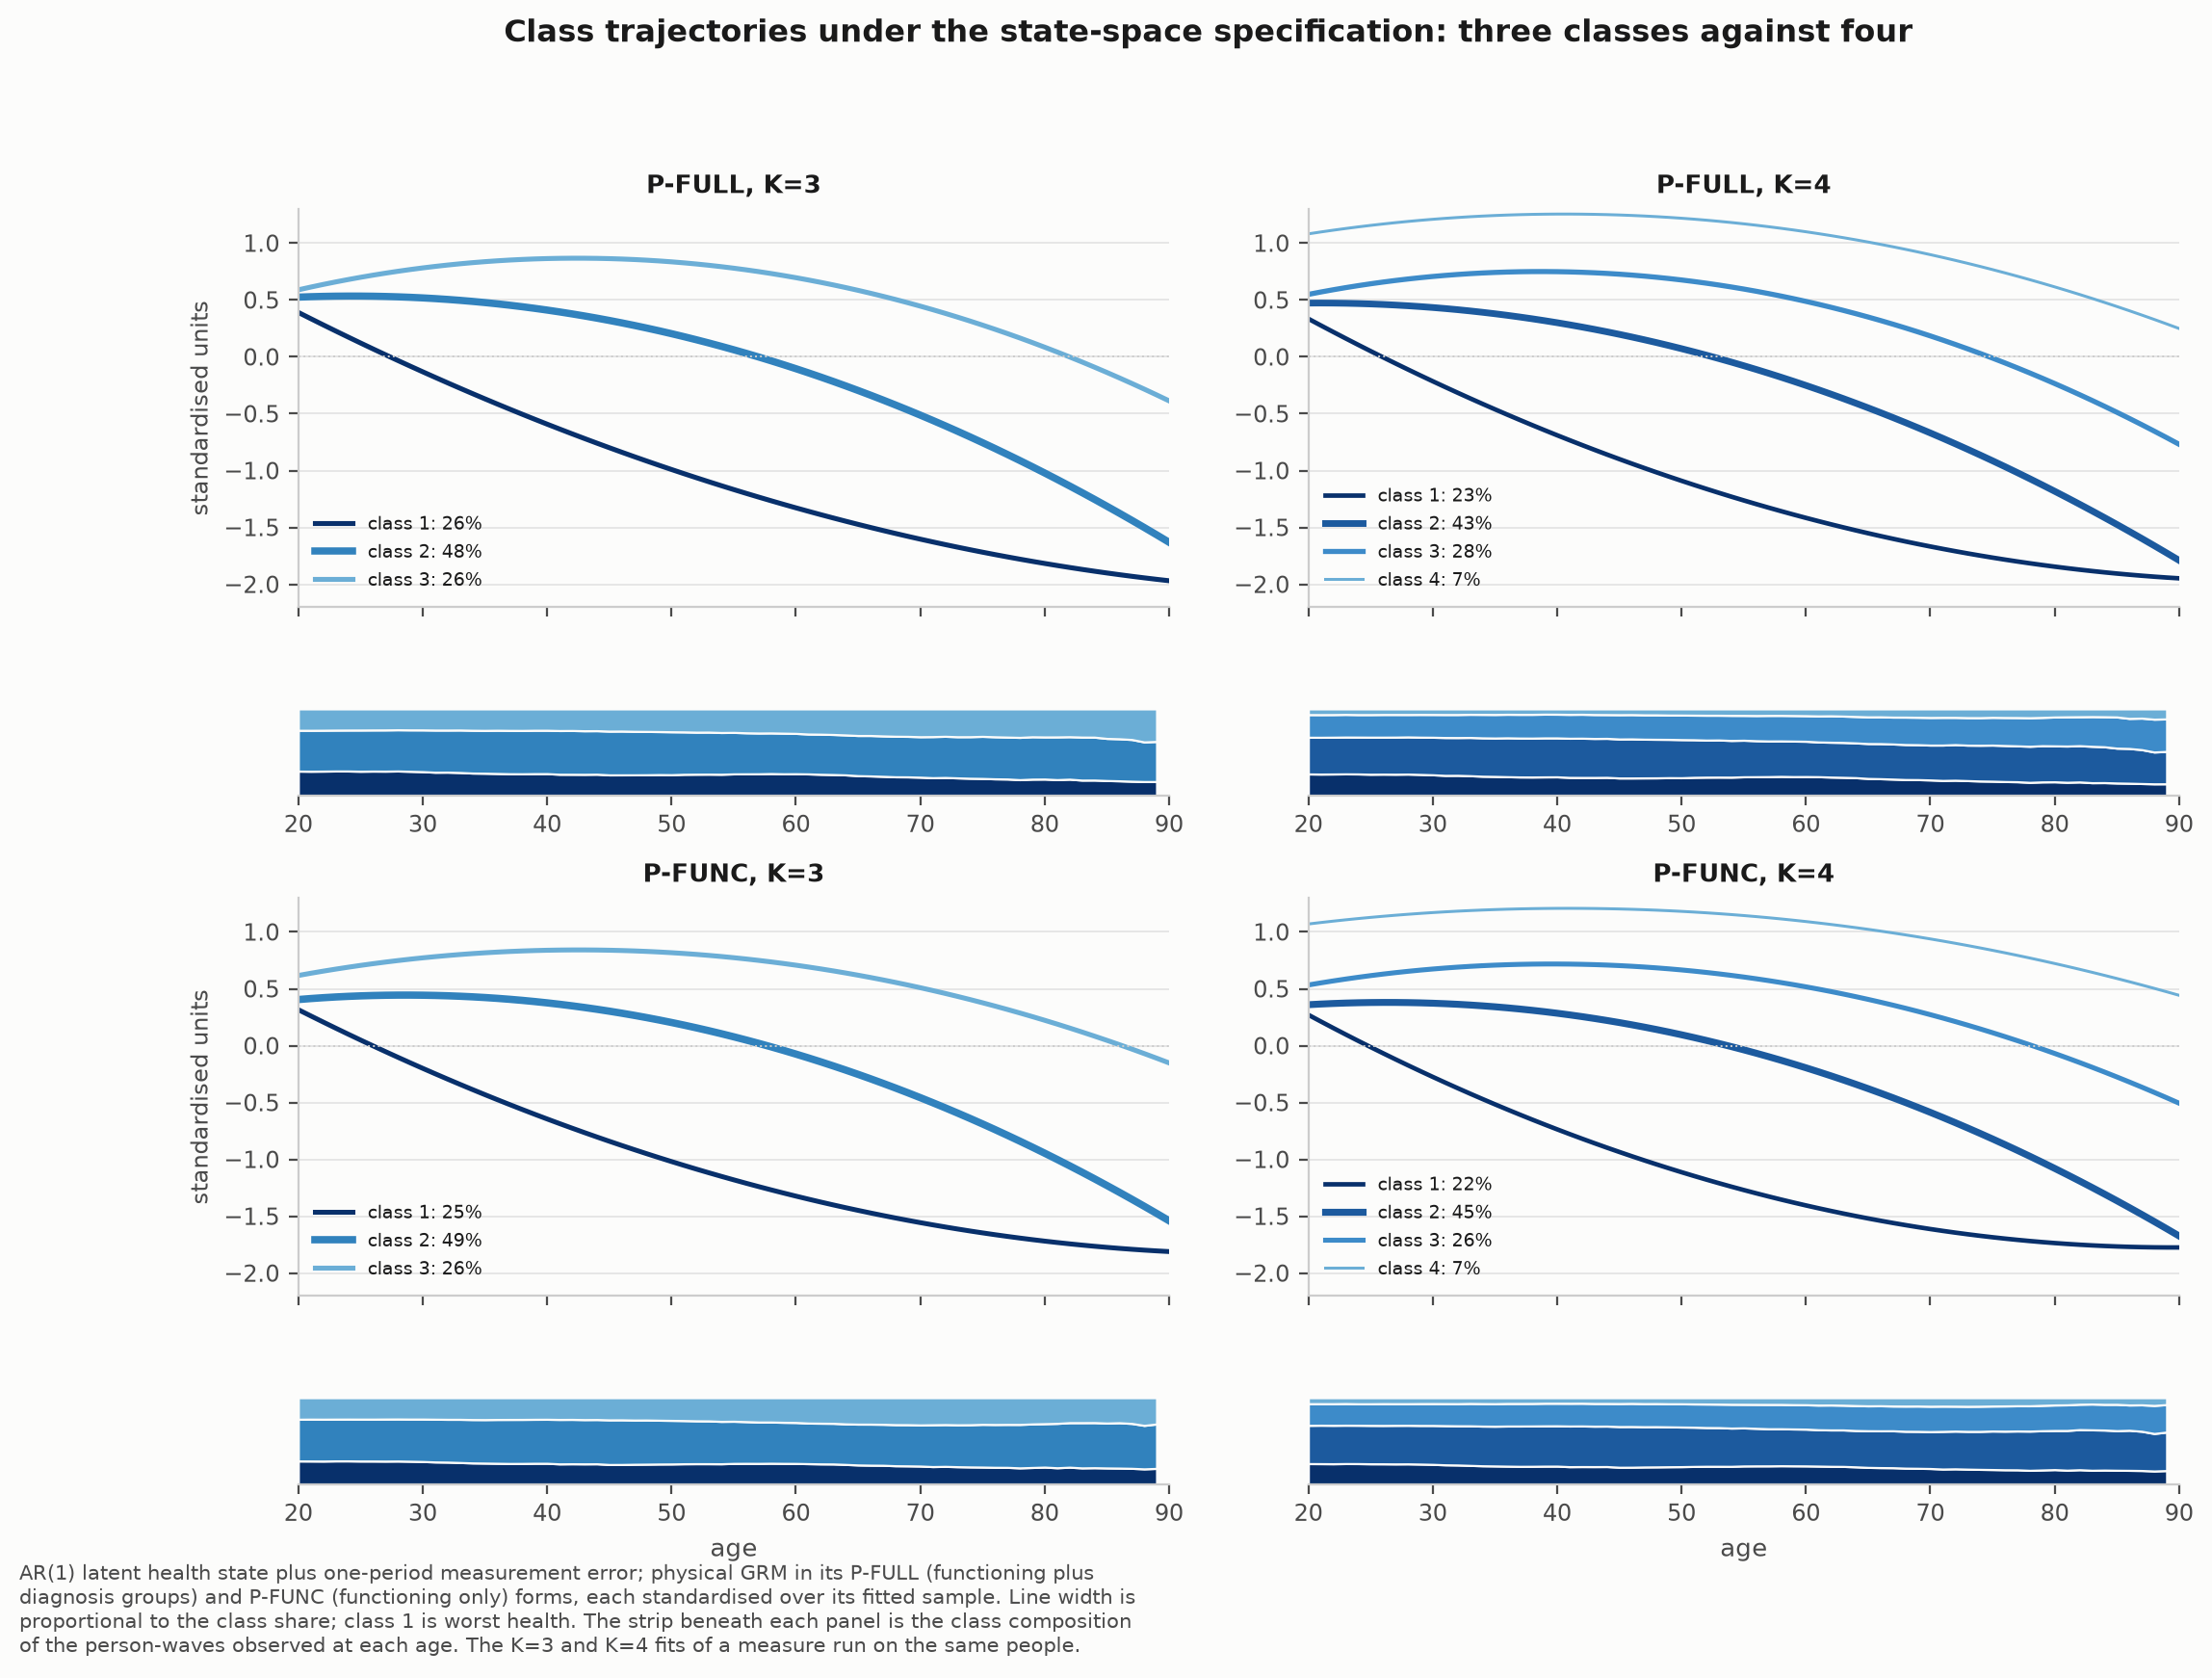
\includegraphics[width=\linewidth]{fig_k4_trajectories}
\caption{Fitted class mean trajectories $\alpha_k + \beta_k a + \gamma_k a^2$
(with $a = (\text{age}-55)/10$) for the state-space specification at three and
four classes. Rows: the physical GRM as P-FULL (\code{theta\_phys\_full},
functioning plus diagnosis groups) and as P-FUNC (\code{theta\_phys\_func},
functioning only), each standardised over its fitted sample. Columns: K=3
and K=4, fitted to the same people. Line width is proportional to the class
share; class 1 is worst health. The strip beneath each panel is the class
composition of the person-waves observed at each age.}
\label{fig:k4traj}
\end{figure}

\begin{center}\small
\begin{tabular}{lrrrrr}
\toprule
Fit & worst-class & \multicolumn{2}{c}{level gap (best $-$ worst)} &
\multicolumn{2}{c}{decline, age 30--80} \\
 & share & age 30 & age 80 & worst & best \\
\midrule
P-FULL, K=3 & .261 & 0.91 & 1.90 & $-1.69$ & $-0.70$ \\
P-FULL, K=4 & .226 & 1.42 & 2.46 & $-1.63$ & $-0.60$ \\
\addlinespace
P-FUNC, K=3 & .254 & 0.97 & 1.94 & $-1.52$ & $-0.55$ \\
P-FUNC, K=4 & .223 & 1.45 & 2.46 & $-1.46$ & $-0.45$ \\
\bottomrule
\end{tabular}

{\scriptsize Standardised units. ``Best'' is class 3 at K=3 and the added
class 4 at K=4, so the gaps are not like-for-like across K.}
\end{center}

\textbf{The first three classes keep their shape.} Classes 1 to 3 at K=4
trace the same paths as the three classes at K=3, shifted slightly down:
the worst class still starts close to the others and falls away fastest
($-1.63$ and $-1.46$ sd from 30 to 80, against $-1.69$ and $-1.52$), and it
shrinks a little, from $.26$ to $.23$. The level gaps widen mainly because the
``best'' class is now a more extreme one; class 3 at K=4 sits at $0.71$ and
$-0.24$ at ages 30 and 80 on P-FULL, close to the K=3 top class's $0.78$ and
$0.09$.

\textbf{The fourth class is high, flat and small.} It starts at $1.21$ sd on
P-FULL ($1.17$ on P-FUNC) and declines only $0.60$ ($0.45$) sd by age 80, the
flattest path in either model. Its share of the person-waves observed at each
age barely moves with age, so unlike the worst class it is not thinned by
attrition.

\begin{center}\small
\begin{tabular}{lrrrrrr}
\toprule
 & share & $\alpha$ & $\rho$ & signal share & level, 30 & level, 80 \\
\midrule
\multicolumn{7}{@{}l}{\emph{P-FULL, K=4}} \\
class 1 & .226 & $-1.26$ & .948 & .77 & $-0.21$ & $-1.85$ \\
class 2 & .425 & $-0.08$ & .892 & .63 & $0.43$ & $-1.18$ \\
class 3 & .278 & $0.60$ & .796 & .48 & $0.71$ & $-0.24$ \\
class 4 & .071 & $1.17$ & .678 & .39 & $1.21$ & $0.62$ \\
\addlinespace
\multicolumn{7}{@{}l}{\emph{P-FUNC, K=4}} \\
class 1 & .223 & $-1.27$ & .943 & .76 & $-0.28$ & $-1.74$ \\
class 2 & .445 & $-0.04$ & .883 & .61 & $0.37$ & $-1.08$ \\
class 3 & .261 & $0.60$ & .737 & .43 & $0.67$ & $-0.07$ \\
class 4 & .071 & $1.14$ & .524 & .32 & $1.17$ & $0.72$ \\
\bottomrule
\end{tabular}

{\scriptsize $\alpha$ is the class level at age 55. Signal share is the
persistent-state share of observation variance,
$\sigma^2/(1-\rho_k^2)$ over that plus $\sigma^2_{\text{meas}}$.}
\end{center}

\subsection*{Where the fourth class comes from}

\begin{figure}[H]
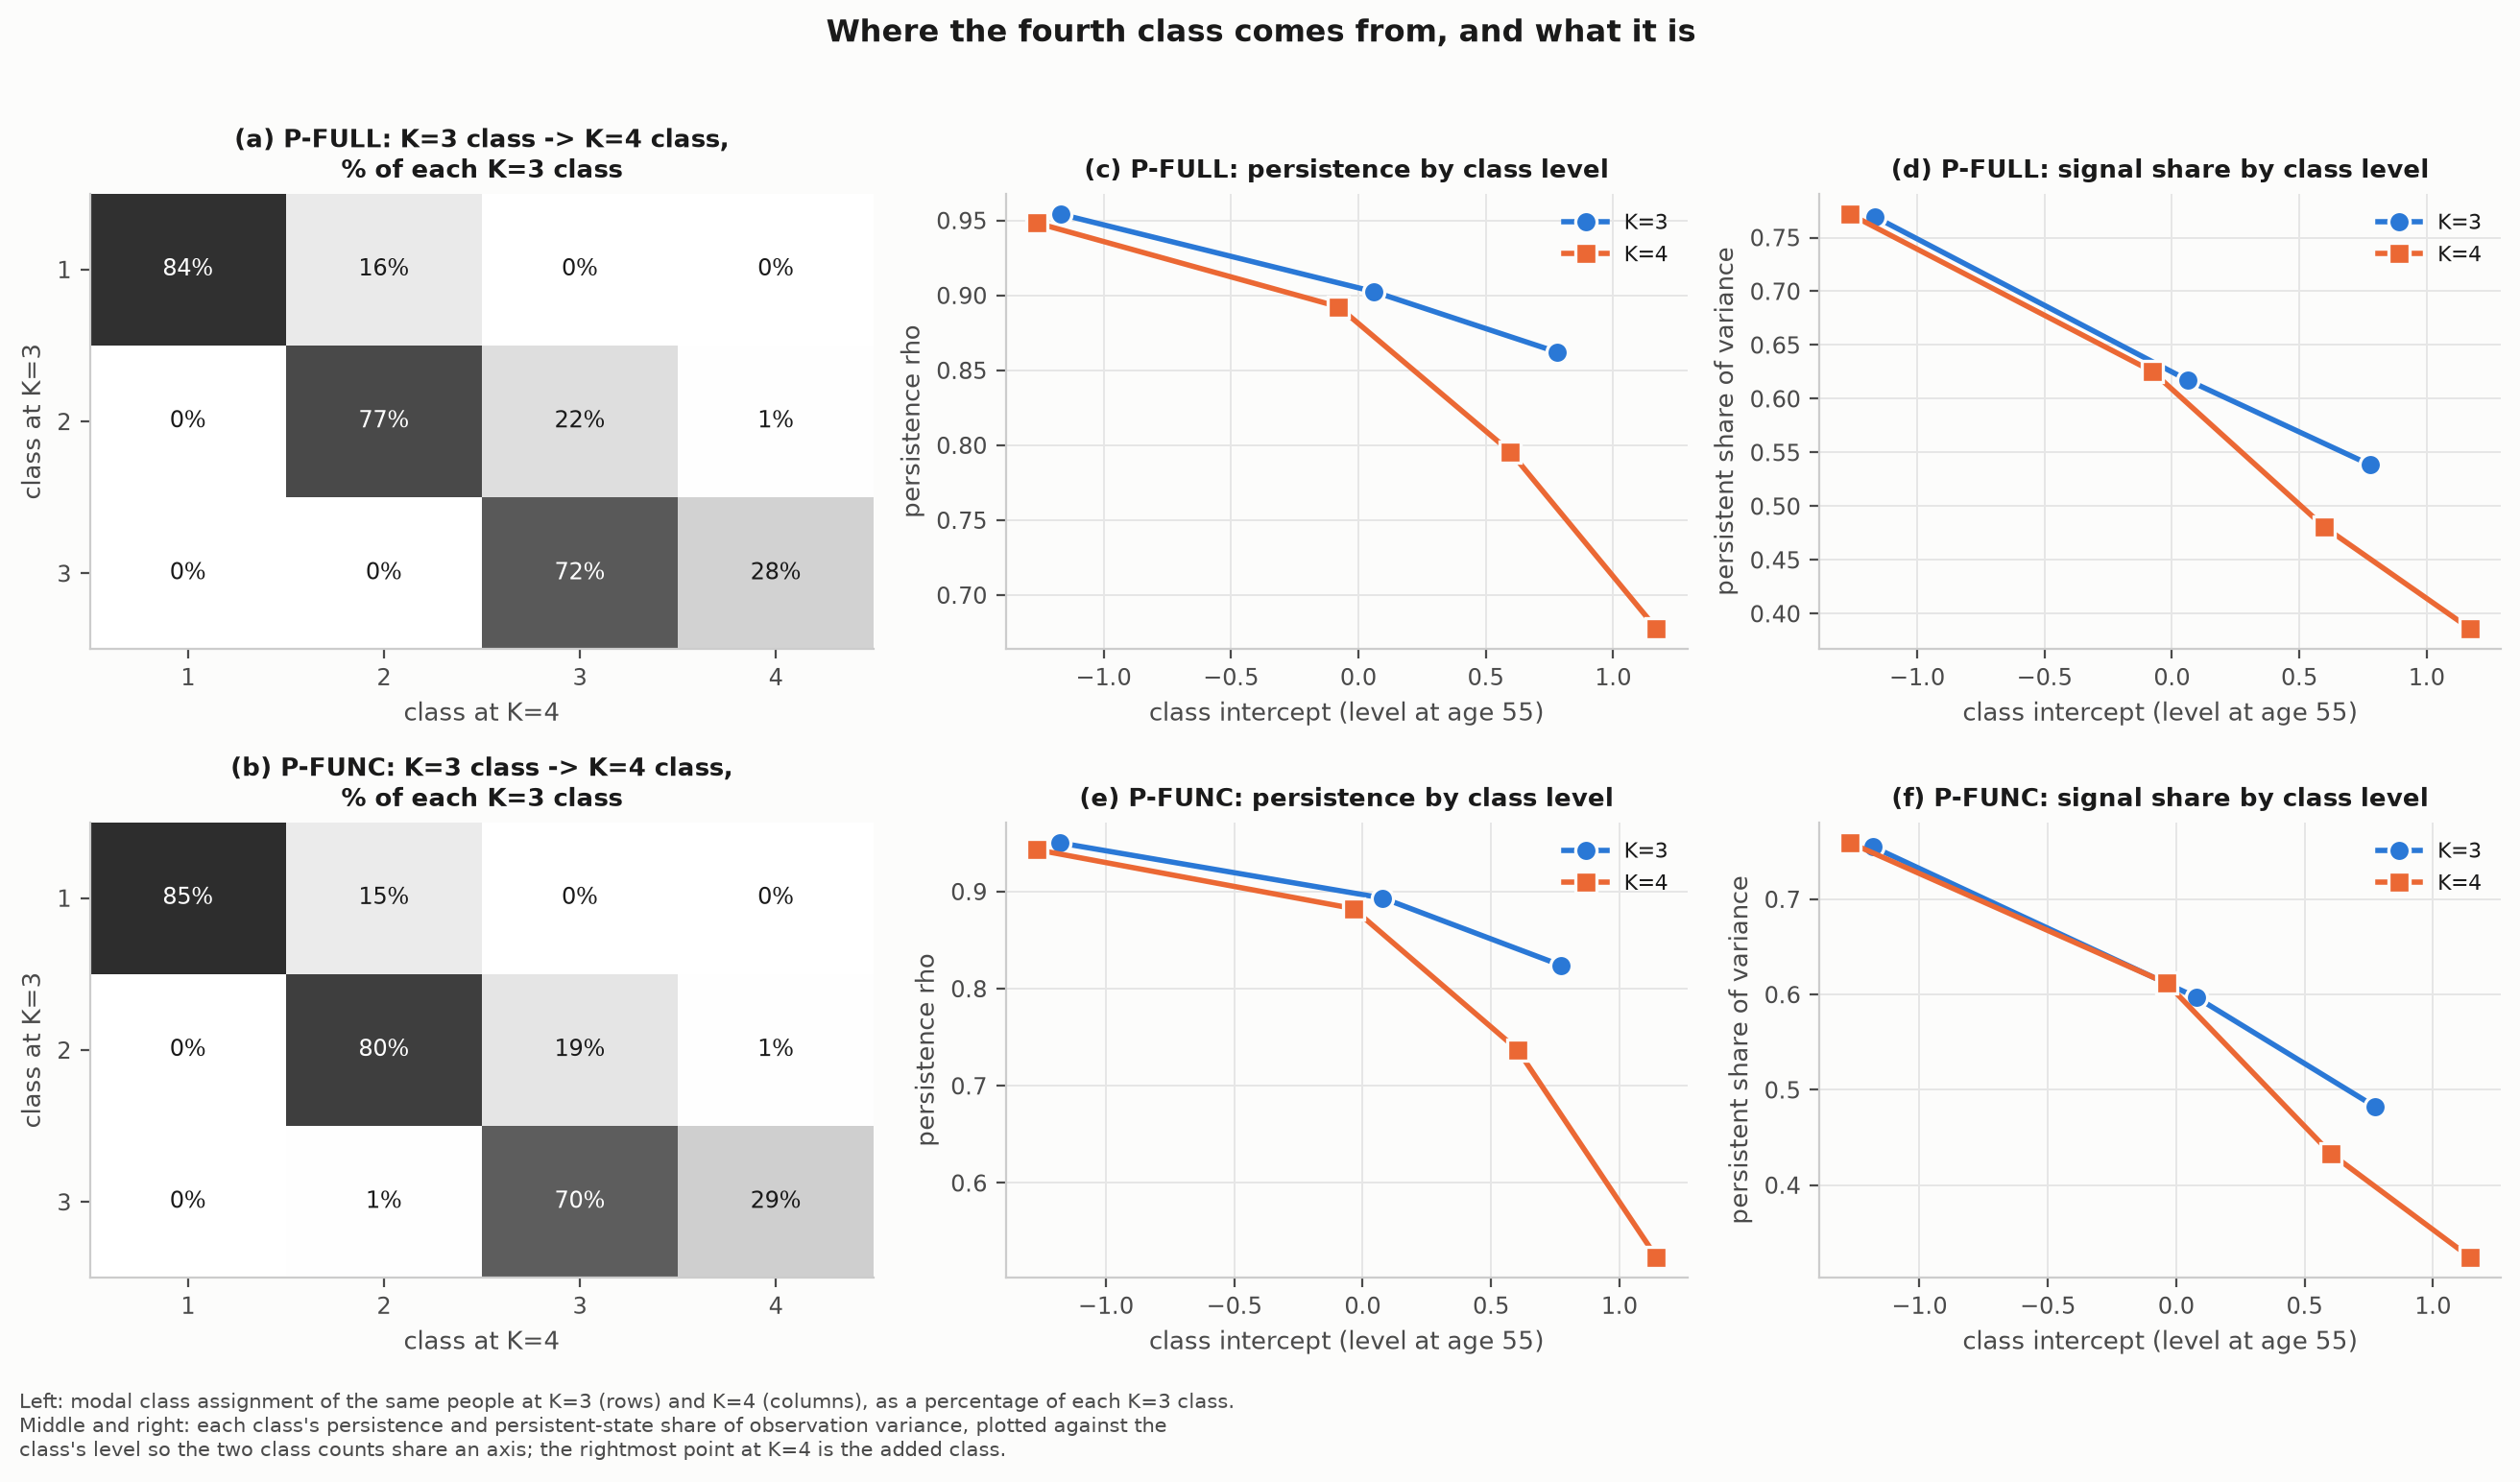
\includegraphics[width=\linewidth]{fig_k4_structure}
\caption{Left, (a) and (b): the modal class of each person at K=3 (rows)
against their modal class at K=4 (columns), as a percentage of each K=3
class; the K=3 and K=4 fits run on the same people, so this is a
person-by-person cross-tabulation. Modal assignment overstates how cleanly
people map --- the posterior-weighted version is more diffuse, see text.
Middle and right, (c) to (f): each class's persistence $\rho$ and signal
share, plotted against the class's level at age 55 so the two class counts
share one axis; the rightmost point at K=4 is the added class.}
\label{fig:k4structure}
\end{figure}

\textbf{It is carved from the top, and every boundary moves up a step.} Of
the people in the healthiest K=3 class, $72\%$ stay in the corresponding K=4
class and $28\%$ move to the new class on P-FULL ($70\%$ and $29\%$ on
P-FUNC). Almost nobody reaches it from lower down: $1\%$ of the middle K=3
class. The lower classes are not simply left alone, though. Each gives up its
healthier members to the class above it --- $16\%$ of the worst K=3 class
moves to K=4 class 2, and $22\%$ of the middle class to K=4 class 3 --- so
adding a class at the top shifts the whole ladder rather than splitting one
rung.

\textbf{Modal assignment makes that look cleaner than it is.} Weighting each
person by their posterior class probabilities instead of their single most
likely class, only $57\%$ of the worst K=3 class's membership lands in K=4
class 1 and $35\%$ in class 2; the top K=3 class splits $49 / 27 / 20$ across
K=4 classes 3, 2 and 4. The typical person is shared between neighbouring
classes at either K, which is the overlap the fit statistics below measure.

\textbf{Persistence and signal share extend the same gradient.} At both K,
$\rho$ and the signal share fall monotonically as class level rises (panels
c to f). The added class carries the lowest of both: $\rho = 0.68$ and a
signal share of $0.39$ on P-FULL, $0.52$ and $0.32$ on P-FUNC. Refitting
also moves a little variation out of the noise term: $\sigma_{\text{meas}}$
falls from $.418$ to $.413$ (P-FULL) and from $.442$ to $.435$ (P-FUNC),
while the state innovation $\sigma$ rises from $.229$ to $.241$ and from
$.242$ to $.257$.

\textbf{The instrument ranking holds.} P-FULL remains the less noisy measure
at K=4, $\sigma_{\text{meas}} = .413$ against $.435$ --- the same ordering as
at K=3, where \S\ref{sec:meas}'s same-roster control showed the gap is a
property of the instrument rather than the sample. The K=4 P-FUNC fit is on
the larger roster, so this particular comparison carries the cross-roster
caveat of \S\ref{sec:meas}, which that control resolved in P-FULL's favour.

\subsection*{Can the model recover a fourth class?}

The real-data fits cannot say whether the model would find a fourth class of
this shape if one truly existed. So a panel of 5{,}000 people was simulated
from the fitted P-FULL K=4 posterior --- class-specific persistence included,
no ceiling imposed --- and refitted with the same model at K=4 (four chains,
1{,}000 warmup and 600 sampling iterations).

\begin{center}\small
\begin{tabular}{lrrrrrrl}
\toprule
 & \multicolumn{2}{c}{share} & \multicolumn{2}{c}{level $\alpha$} &
\multicolumn{3}{c}{persistence $\rho$} \\
\cmidrule(lr){2-3}\cmidrule(lr){4-5}\cmidrule(lr){6-8}
Class & truth & estimate & truth & estimate & truth & estimate & 90\% interval \\
\midrule
1 & .226 & .200 & $-1.02$ & $-1.14$ & .948 & .939 & .927--.949 \\
2 & .425 & .409 & $0.08$ & $-0.00$ & .893 & .887 & .856--.914 \\
3 & .278 & .299 & $0.70$ & $0.66$ & .796 & .789 & .736--.836 \\
4 & .071 & .093 & $1.23$ & $\mathbf{1.14}$ & .678 & $\mathbf{.765}$ & .706--.814 \\
\bottomrule
\end{tabular}

{\scriptsize On the simulated panel's standardised scale. $\sigma$ is
recovered as $.223$ against $.223$, $\sigma_{\text{meas}}$ as $.383$ against
$.383$. Bold marks the two parameters, of 22, whose true value falls outside
the 90\% posterior interval.}
\end{center}

\textbf{It does.} The fit converges cleanly --- maximum $\hat R$ $1.008$, no
divergences, and the four chains agree on every persistence parameter to
within $.009$, so there is no mode split. The true value lies inside the 90\%
interval for 20 of the 22 parameters, about the rate expected. The fourth
class comes back at the right size and in the right place: a share of $.093$
against $.071$, inside its interval. The fitted fourth class is therefore not
an artefact of the estimation: were such a class real, this model would find
it.

\textbf{Its persistence is overstated, in a telling direction.} Both misses
are in the fourth class. Its level is understated ($1.14$ against $1.23$) and
its persistence overstated ($.765$ against $.678$, with the truth below the
interval). A third of the people truly in the fourth class ($31.6\%$) are
assigned to class 3, which is more persistent, and the estimate is pulled
towards its neighbour. The real fit has roughly eight times as many people,
so the pull there should be weaker; but its direction means the real fourth
class's persistence of $.68$ is, if anything, itself an overstatement. The
class is not more persistent than it appears.

\textbf{A true fourth class is no easier to assign.} At the \emph{true}
parameters the average person's most likely class has probability $.689$
(relative entropy $.504$), and only $69\%$ of people are assigned to the class
they were simulated in; at the estimates, $.711$ and $69\%$. That is the
overlap this configuration produces when four classes are genuinely present:
a persistent state blurred by one-period noise leaves neighbouring classes
indistinguishable for many people. Members of the true fourth class are found
about as often as anyone else ($68\%$, against $59\%$ for the worst class).

\subsection*{Does the fourth class earn its place?}

\begin{center}\small
\begin{tabular}{llrrrrr}
\toprule
Measure & K & log likelihood & parameters & BIC &
\multicolumn{2}{c}{classification} \\
 & & & & & mean max.\ posterior & relative entropy \\
\midrule
P-FULL & 3 & $-295{,}489.9$ & 16 & $591{,}149$ & .696 & .403 \\
P-FULL & 4 & $-295{,}203.4$ & 21 & $590{,}629$ & .668 & .478 \\
\addlinespace
P-FUNC & 3 & $-404{,}460.7$ & 16 & $809{,}095$ & .704 & .421 \\
P-FUNC & 4 & $-403{,}963.2$ & 21 & $808{,}154$ & .679 & .495 \\
\bottomrule
\end{tabular}

{\scriptsize In-sample marginal log likelihood at the posterior-mean
parameters, class states integrated out by the Kalman filter. BIC uses the
number of people. Mean max.\ posterior is the average probability of each
person's most likely class; relative entropy is $1 - \text{entropy}/(N\ln K)$.}
\end{center}

\textbf{On fit, yes --- but at this sample size that settles little.} Four
classes raise the log likelihood by $287$ (P-FULL) and $498$ (P-FUNC) for five
extra parameters, and BIC prefers K=4 by $520$ and $941$. But a penalty of
five parameters costs only about $27$ log-likelihood units at this sample
size ($5\ln N/2$), against gains of $287$ and $498$, so BIC is weighing little here and is
not the test that matters. Larger K has not been fitted.

\textbf{On separation, the statistics cannot decide.} People are assigned
slightly less confidently at K=4: the average probability of each person's
most likely class falls from $.696$ to $.668$ on P-FULL and from $.704$ to
$.679$ on P-FUNC. Relative entropy moves the other way, from $.40$ to $.48$,
but only because it divides by $\ln K$. Neither is high at either K ---
relative entropies of $.40$--$.50$ fall well short of the values near $.8$
usually read as clean separation --- but the recovery check shows that a
genuine four-class population of this shape yields $.69$ at its true
parameters. Certainty in this range is what a real fourth class would produce
as well, so it is not evidence against one.

\textbf{And the added class sits at the measurement ceiling.} A sizeable
share of the physical GRM is piled at its maximum, and that mass is
concentrated in exactly the people the fourth class describes:

\begin{center}\small
\begin{tabular}{lrrrr}
\toprule
 & \multicolumn{2}{c}{P-FULL} & \multicolumn{2}{c}{P-FUNC} \\
Person-mean level (sd) & people & waves at maximum & people & waves at maximum \\
\midrule
$\ge 1.0$ & 3{,}862 & $\mathbf{45.6\%}$ & 4{,}322 & $\mathbf{58.8\%}$ \\
$0.5$ to $1.0$ & 8{,}733 & $8.9\%$ & 11{,}517 & $13.8\%$ \\
$0$ to $0.5$ & 9{,}621 & $2.0\%$ & 12{,}566 & $3.5\%$ \\
below $0$ & 16{,}747 & $0.3\%$ & 21{,}596 & $0.5\%$ \\
\midrule
all person-waves & & $6.8\%$ & & $9.3\%$ \\
\bottomrule
\end{tabular}

{\scriptsize Share of each person's observations recorded at the measure's
exact maximum, by the person's mean standardised level, in the fitted
lifecycle sample; hence $6.8\%$ and $9.3\%$ overall rather than
\S\ref{sec:ceiling}'s whole-panel $7.2\%$ and $9.5\%$.}
\end{center}

People at the fourth class's level have close to half of their observations
recorded at the exact maximum. The model treats observations as Gaussian and
has no notion of a ceiling, so a score that alternates between the maximum
and just below it can only be read as transient noise around a weakly
persistent state --- which is precisely the fourth class's signature: the
lowest $\rho$ and the lowest signal share of any class. The two measures line
up the same way. P-FUNC, which piles more people at its ceiling ($58.8\%$
against $45.6\%$), gives its fourth class markedly lower persistence ($0.52$
against $0.68$) and signal share ($0.32$ against $0.39$). That is what a
ceiling artefact predicts, and it echoes \S\ref{sec:ceiling}, where the
diagnosis items were found to relieve the ceiling on P-FULL.

\textbf{Reading.} The fourth class is not an estimation artefact. It is
recovered at the same size and position by two measures, it converges
cleanly, it improves the in-sample fit, and simulation shows the model finds
a class of this shape when one is truly there. What tells against reading it
as a distinct trajectory is the ceiling, and the ceiling alone: its defining
dynamics are the ones a measurement ceiling produces, and about half of its
members' observations sit at the exact maximum. The classification statistics
bear on the question neither way. It is best read as the people at the top of
the physical GRM's range, whose recorded health cannot rise further, rather
than as a distinct lifecycle trajectory. That is informative
in its own right --- it locates where measurement rather than health drives
the estimated dynamics --- but it is not a reason to prefer four classes to
three for describing health trajectories, and the rest of this note keeps
K=3.

\textbf{What is not established.} The recovery check shows that the model
can find a fourth class, not that the real one is genuine: it was run without
a ceiling, so it tests the model rather than the ceiling reading. It also used
5{,}000 people, an eighth of the fitted sample, so the size of the persistence
bias it found is not the size in the real fit. There is no AR(1) fit at K=4,
so \S\ref{sec:meas}'s same-sample attenuation contrast cannot be repeated, and
no holdout, so whether K=4 predicts better out of sample is unknown. The
ceiling reading therefore remains an interpretation of the pattern rather than
a test of it. The direct tests would be to repeat this simulation from
\emph{three} true classes with scores censored at the measure's maximum and
see whether a small, weakly persistent top class appears, or to fit an
observation model that treats scores at the maximum as censored.

\section{Towards a multidimensional model}
\label{sec:multidim}

The predecessor's five-channel mixed model used PCS and MCS (Gaussian),
self-rated health (ordered logit), a chronic count (negative binomial) and an
ADL count (hurdle negative binomial). Everything in this note argues for a
different set, and the binding constraint is coverage.

\begin{center}\small
\begin{tabular}{lrrl}
\toprule
Candidate channel & person-waves & persons & limiting gate \\
\midrule
$\theta$ physical, P-FUNC & 497{,}423 & 84{,}679 & none (every wave) \\
$\theta$ mental, without DEPR & 489{,}278 & 81{,}729 & none (every wave) \\
$\theta$ mental, as fitted (with DEPR) & 379{,}462 & 67{,}017 & diagnosis inventory \\
$\theta$ physical, P-FULL & 387{,}599 & 69{,}958 & diagnosis inventory \\
chronic count & \multicolumn{2}{c}{$76\%$ of person-waves} & diagnosis inventory \\
ADL count & \multicolumn{2}{c}{4 waves ($\sim 8\%$)} & scheduled module \\
\bottomrule
\end{tabular}
\end{center}

\textbf{One weak item is costing a quarter of the sample.} The mental bank as
fitted includes ever-diagnosed depression, which inherits the BHPS exclusion
of \S\ref{sec:routing}. Dropping that single item --- one hurdle, $a =
0.93$, the weakest item in the bank bar the rare diagnoses --- recovers
109{,}816 person-waves and 14{,}712 people, a $22.4\%$ increase. Jointly
observing a physical and a mental channel then covers 484{,}832 person-waves
on 81{,}458 people (49{,}545 of them with three or more observations),
against 376{,}019 / 66{,}841 / 38{,}478 if either channel carries a
diagnosis item. That is a $29\%$ larger estimation sample for the loss of
almost no information.

\textbf{Recommended specification.} Three channels, and the ragged-channel
machinery already in \code{runner/mixed.py} handles them as they stand:

\begin{enumerate}\itemsep2pt
\item \textbf{$\theta$ physical (P-FUNC)}, Gaussian. Replaces PCS and,
because self-rated health enters as the GH item and functioning as FUNC, it
also absorbs the old model's separate self-rated-health channel and its ADL
channel --- the latter traded for \code{disdif}, which measures the same
construct in every wave rather than four.
\item \textbf{$\theta$ mental without DEPR}, Gaussian. Replaces MCS, without
the orthogonality artifact, and with GHQ-12 doing most of the work.
\item \textbf{Chronic condition count}, negative binomial, on the $76\%$ of
person-waves where the inventory exists. Kept as a channel rather than folded
into a measurement model, which is where \S\ref{sec:ever} concluded it
belongs: ``ever'' is the correct state variable for a diagnosis, its
accumulation is a process to be modelled rather than an artefact to be
corrected, and as a channel its missingness is explicit instead of silently
deleting people.
\end{enumerate}

Two properties of this design matter. First, the class structure is
identified off channels 1 and 2, which are observed for everyone in every
wave, so the BHPS members contribute to the typology even though channel 3 is
missing for them --- the opposite of the current arrangement, where they are
dropped outright. Second, the missingness in channel 3 is a survey-design
gate, not a health-related process: the excluded people are indistinguishable
on every health measure (\S\ref{sec:routing}), so treating it as ignorable
conditional on the observed channels is defensible in a way that ADL's
scheduled-module missingness also is, but that attrition would not be.

\textbf{What to leave out, and why.} Utilisation (\S\ref{sec:convexity}) is
an outcome for validating the measures, not a health dimension to be
clustered on. SF-6D is a mixed physical--mental utility
(\S\ref{sec:combined}) and would duplicate both channels at once. The
combined GRM is physically dominated (Figure~\ref{fig:combmodel}) and its
residuals say the data want two dimensions, not one. SWEMWBS, loneliness and
the ADL module all fail the every-wave rule.

\textbf{An extension worth considering later.} Channels 1 and 2 currently
compress each domain to a point estimate and then treat it as data, discarding
the posterior sd the GRM already computes (\S\ref{sec:ceiling}: $0.27$ near
the population mean, rising to $0.65$ at the extremes). Passing that through
as a known measurement-error variance per observation is a small change to
the Gaussian channels and would stop the model reading heteroskedastic
measurement noise as heterogeneity in health --- which, given the ceiling and
floor results, is concentrated exactly in the classes the model cares most
about.

\section{The multidimensional model}
\label{sec:multifit}

The specification of \S\ref{sec:multidim} was fitted in four variants ---
baseline, holdout, AR(1), AR(1)+holdout --- on one common sample of 38{,}268
people and 388{,}774 person-waves, so the four differ by specification alone.
Three channels: the physical GRM (P-FUNC) and the mental GRM without DEPR,
both Gaussian, and the chronic count as a negative binomial, masked on the
$24\%$ of rows with no diagnosis inventory. Mortality was toggled off for
these four fits; it is switched on in the later fits reported under
\emph{Measurement error and mortality} below. All four converged.

\begin{center}\small
\begin{tabular}{lrlllr}
\toprule
Variant & max $\hat R$ & $\theta$ (shares) & $\rho$ & chronic at 55 & wall \\
\midrule
baseline & 1.0032 & .189 / .377 / .434 & --- & 2.6 / 1.4 / 0.13 & 8.0 h \\
holdout & 1.0049 & .187 / .371 / .442 & --- & 2.6 / 1.4 / 0.14 & 6.8 h \\
AR(1) & 1.0014 & .190 / .398 / .413 & .73 / .61 / .60 & 2.9 / 1.1 / 0.01 & 19.0 h \\
AR(1) + holdout & 1.0023 & .195 / .389 / .416 & .72 / .58 / .58 & 2.9 / 1.1 / 0.01 & 18.2 h \\
\bottomrule
\end{tabular}

{\scriptsize ``chronic at 55'' is the implied mean condition count at age 55
for each class.}
\end{center}

\textbf{Extra channels stabilise the classes against the AR term.} In the
univariate fits of \S\ref{sec:ar1} adding persistence roughly doubled the
worst class (.16 $\to$ .33 on both GRM channels). Here the shares are flat
across all four variants at about .19 / .38 / .42. The mechanism in
\S\ref{sec:ar1} was that a single channel cannot separate a small extreme
class from the autocorrelation of repeated low observations, so once $\rho$
can absorb the latter the boundary moves; with three channels the class is
identified from agreement \emph{across} channels, and persistence no longer
competes for the same variation.

\textbf{Persistence is much less class-graded than the univariate fits
implied.} $\rho = .73 / .61 / .60$ here, against $.78 / .27 / .39$ for the
physical GRM alone. The worst class remains the most persistent, but the
other two are far more so once a second correlated channel is observed: a
shock that looks transient in one measure reads as persistent when two move
together. That is a warning about reading $\rho$ off a single channel.

\textbf{The classes absorb the overdispersion in the chronic count.} The
implied means at 55 --- $2.6 / 1.4 / 0.13$ conditions --- weight up to $1.08$
against an observed mean of $1.045$, so the mixture reproduces the marginal.
And \code{phi\_chronic} settles at $656$ (baseline) to $920$ (AR), which for
a negative binomial is effectively Poisson: after conditioning on class and
age there is almost no overdispersion left to model.

\begin{figure}[H]

\includegraphics[width=\linewidth]{fig_multidim_trajectories}
\caption{Class trajectories and shares for the four multidimensional fits,
one row per variant and one column per channel. A fit has a single class
structure, so the shares are identical across a row and the line width
(proportional to the share) repeats; what changes across the row is what each
class \emph{does} on each channel. The Gaussian channels are returned to the
original GRM $\theta$ scale using each fit's standardising moments; the count
channel shows the implied mean number of conditions. Class 1 is worst
physical health by the anchor convention. Together with
Figure~\ref{fig:trajectories}, which covers the eight univariate fits, every
Bayesian model in this note has its trajectories and shares drawn.}
\label{fig:multitraj}
\end{figure}

Figure~\ref{fig:multitraj} makes the classes legible as types rather than as
parameter vectors. The physical channel behaves as the univariate fits led us
to expect: three ordered, non-crossing, accelerating declines, with class 1
falling from about $-0.1$ at age 20 to $-1.7$ at 90 while class 3 stays near
$+0.5$ until the sixties. The mental channel is where the multidimensional
model earns its keep. Its trajectories \emph{rise} with age for every class,
recovering the late-life wellbeing pattern of Figure~\ref{fig:moments} inside a
model that is simultaneously fitting a steep physical decline --- and they
rise fastest for class 3, so the healthiest physical type is also pulling
away mentally. Class 1 is worst on both channels at every age, which is worth
stating because nothing in the model forces it: only the physical channel
carries the ordering constraint, so the mental ordering is an estimate. The
count channel then separates the classes most sharply of the three, from
about $4.5$ conditions at age 80 in class 1 to $0.7$ in class 3.

The composition strips answer a question the shares alone cannot. In a
mixture $\theta$ is a lifetime constant, so any movement in a strip is
selection into the observed sample, not people changing class. Across the
twelve fits that movement is modest but consistent in sign for the physical
measures: the worst class rises from $12.1\%$ of person-waves at age 30 to
$18.8\%$ at 80 on the PCS, and from $29.8\%$ to $34.5\%$ on P-FULL under
AR(1) --- the healthiest are observed at every age while the least healthy
accumulate in the older cells. The multidimensional baselines tilt the other
way ($21.0\%$ at 30 falling to $15.3\%$ at 80), which is mortality and
attrition removing the sickest, and a reminder that these strips describe who
is present rather than how anyone's health evolved.

\subsection*{Held-out prediction, channel by channel}

Chronic is nearly free to predict --- carrying the last observed count
forward is exactly right on $93.4\%$ of the 58{,}600 held-out chronic rows
--- so a single held-out number would be flattered by it. The density is
therefore decomposed by channel offline, validated by reproducing the fits'
own stored per-person values (correlation $0.999999$, maximum deviation
$0.04$).

\begin{center}\small
\begin{tabular}{lrrr}
\toprule
 & \multicolumn{2}{c}{AR(1) + holdout} & holdout \\
Channel & AR-conditional & class-only & (no AR) \\
\midrule
$\theta$ physical & $-0.936$ & $-1.059$ & $-1.121$ \\
$\theta$ mental & $-1.138$ & $-1.245$ & $-1.321$ \\
chronic count & $-0.981$ & $-0.981$ & $-1.086$ \\
\midrule
all three & $-1.021$ & $-1.105$ & $-1.184$ \\
\bottomrule
\end{tabular}

{\scriptsize Log predictive density per held-out row. 76{,}536 rows on each
Gaussian channel, 58{,}623 on the count.}
\end{center}

Three readings. First, the two Gaussian channels gain $0.12$ and $0.11$ nats
per row from carrying the last value forward, while \textbf{the chronic
channel gains exactly zero} --- to three decimal places, because the model
carries no persistence term on that channel at all. It predicts the count
from class and age, never from the person's own previous count.

Second, that omission is expensive. The distribution of the change from a
person's last observed count is $93.4\%$ zero, $5.8\%$ $+1$, $0.6\%$ $+2$ or
more, with an entropy of $0.274$ nats. A channel that used the previous count
could therefore reach about $-0.27$ per row where the fitted model achieves
$-0.98$: roughly \textbf{0.7 nats per row left on the table}, far more than
the $0.12$ the AR term buys on the Gaussian side. This is the count-channel
analogue of the generated-quantities defect of \S\ref{sec:gqfix}, and the
obvious next fix: the chronic channel should condition on the last observed
count, either as an offset or through a monotone accumulation process.

Third, the physical channel predicts better than the mental one on every
variant ($-0.94$ against $-1.14$), the same ordering the univariate fits
found, and the non-AR holdout has AR-conditional and class-only densities
identical to four decimal places --- correct by construction when there is no
persistence to carry, and a useful check that the toggle behaves.

\subsection*{Measurement error and mortality}
\label{sec:multimort}

Three further multidimensional fits were run on the same 38{,}268 people and
388{,}774 person-waves: the state-space specification of \S\ref{sec:meas} on
both Gaussian channels, with and without the mortality hazard, and the
mortality hazard on the conditionally independent baseline. Measurement error
enters the two GRM channels only. A condition count is a report of an
accumulated stock rather than a noisy reading of a continuous state, and
mortality is administrative, so neither has a measurement-error analogue.
Mortality is a per-wave logit hazard with a quadratic in age, observed on
every person-wave, with 1{,}996 deaths among the 38{,}268 people.

\textbf{Both state-space fits split into two modes.} The ordering constraint
sits on the physical-GRM intercept, but under this specification classes 2
and 3 differ mainly on the chronic channel and lie close on the physical one.
A chain that starts with those two labels the wrong way round cannot exchange
them without crossing the constraint, so it settles against the boundary with
the two intercepts pressed together --- a gap of $0.000$, against $0.32$ in
the other chains. That mode sits $480$ log-posterior units below the other in
both fits, so it is decisively worse rather than a competing account of the
data, but pooling chains across the two modes produced split $\hat R$ values
up to $54$. Relabelling does not repair it, because a trapped chain sits at
different parameter values rather than at a permutation of the same ones. The
state-space results below therefore use only the chains in the better mode ---
three of four without mortality, two of four with --- on which split $\hat R$
is $1.003$ and $1.004$. The baseline with mortality converged without a split
on all four chains ($\hat R$ $1.001$). The durable fix is to put the ordering
constraint on the channel that actually separates the classes; until that is
done the two state-space fits should be treated as provisional.

\begin{center}\small
\begin{tabular}{lrrlllr}
\toprule
Variant & chains & max $\hat R$ & $\theta$ (shares) & $\rho$ &
$\sigma_{\text{meas}}$ & wall \\
\midrule
baseline & 4 & 1.003 & .189 / .377 / .434 & --- & --- & 8.0 h \\
baseline + mortality & 4 & 1.001 & .189 / .377 / .434 & --- & --- & 13.2 h \\
AR(1) & 4 & 1.001 & .190 / .398 / .413 & .73 / .61 / .60 & --- & 19.0 h \\
AR(1)+ME & 3 of 4 & 1.003 & .171 / .413 / .416 & .96 / .94 / .93 & .445 / .549 & 35.1 h \\
AR(1)+ME + mortality & 2 of 4 & 1.004 & .171 / .413 / .416 & .96 / .94 / .93 & .445 / .549 & 37.3 h \\
\bottomrule
\end{tabular}

{\scriptsize ME: AR(1) latent state plus one-period measurement error on the
two Gaussian channels; $\sigma_{\text{meas}}$ is physical / mental.
``chains'' is the number used; for the state-space fits
the rest were in the inferior mode. Implied condition counts at 55 are
$2.6 / 1.4 / 0.13$ for both baselines and $3.1 / 1.1 / 0.01$ for both
state-space fits.}
\end{center}

\textbf{The univariate finding carries into the joint model.} Separating
measurement error lifts persistence from $.73 / .61 / .60$ to
$.96 / .94 / .93$. The innovation scale falls from $0.60$ and $0.71$ to $0.23$
and $0.25$ on the physical and mental channels, and measurement error takes up
$0.445$ and $0.549$ respectively. The mental GRM is the noisier instrument, in
line with its weaker held-out prediction above. And persistence becomes
almost flat across the classes, as the univariate state-space fits of
\S\ref{sec:meas} found on a single channel.

\textbf{Mortality is strongly graded by class, and changes nothing else.}

\begin{center}\small
\begin{tabular}{lrrrrrr}
\toprule
 & \multicolumn{3}{c}{baseline + mortality} & \multicolumn{3}{c}{AR(1) + ME + mortality} \\
\cmidrule(lr){2-4}\cmidrule(lr){5-7}
Class & age 55 & age 70 & age 85 & age 55 & age 70 & age 85 \\
\midrule
1 & 0.53\% & 2.18\% & 8.58\% & 0.52\% & 2.01\% & 8.62\% \\
2 & 0.17\% & 0.88\% & 5.79\% & 0.14\% & 0.78\% & 5.66\% \\
3 & 0.08\% & 0.46\% & 3.53\% & 0.08\% & 0.48\% & 3.74\% \\
\bottomrule
\end{tabular}

{\scriptsize Probability of dying in a wave, from the class-specific logit
hazard at posterior-mean parameters. Class 1 is worst health.}
\end{center}

\begin{figure}[H]
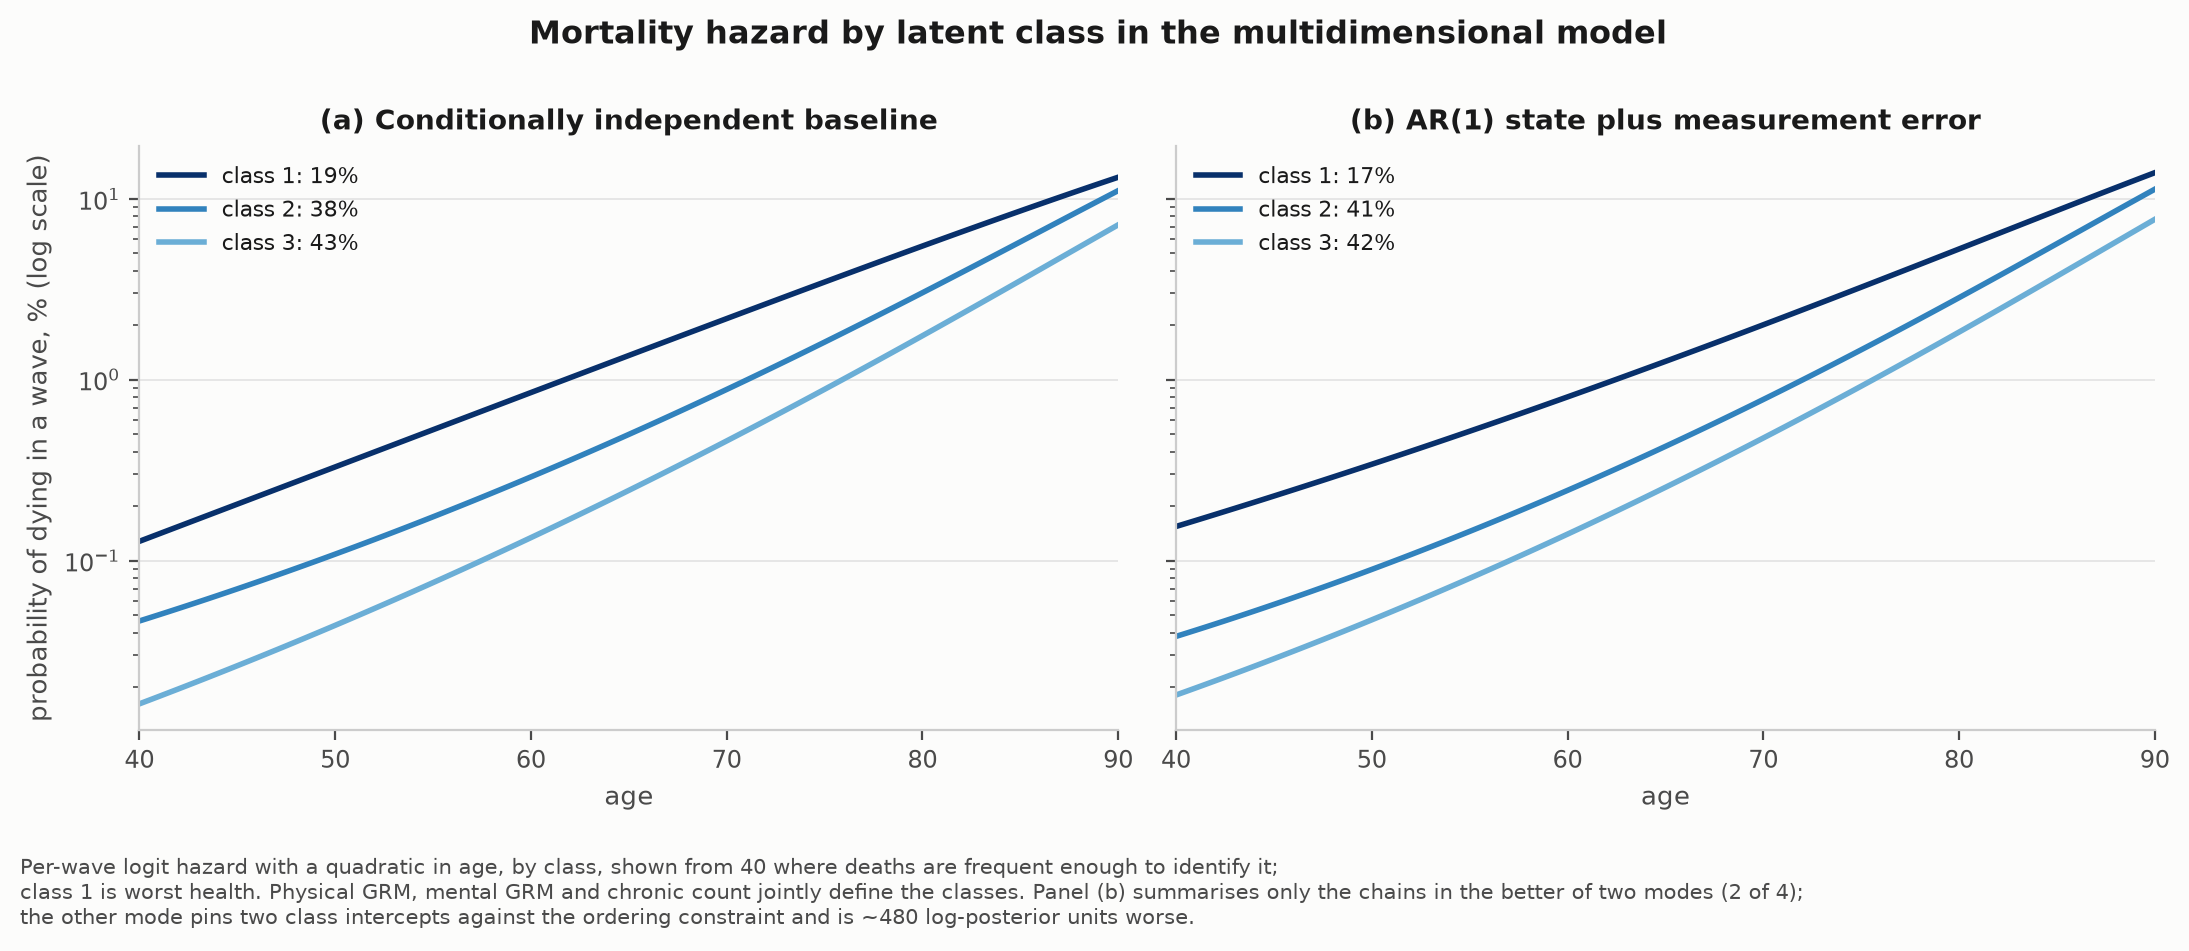
\includegraphics[width=\linewidth]{fig_multidim_mortality}
\caption{Per-wave mortality hazard by latent class in the multidimensional
model (physical GRM as P-FUNC, mental GRM without DEPR, chronic count), on a
log scale from age 40, below which deaths are too few to identify the age
quadratic. Panel (a): conditionally independent baseline, all four chains.
Panel (b): AR(1) latent state plus measurement error, the two chains in the
better mode.}
\label{fig:multimort}
\end{figure}

At age 55 a person in the worst class is $7.0$ times as likely (on the odds
scale) to die in a given wave as one in the healthiest, and $6.5$ times under
measurement error. The hazards converge with age: by 85 the gap is $8.6\%$
against $3.5\%$, or $2.4$ times. The two specifications agree closely on all
of it. Adding the channel leaves the typology exactly as it was: shares,
intercepts and chronic profiles agree to three decimal places with and without
mortality, on both specifications. With 1{,}996 deaths set against 777{,}548
Gaussian and 295{,}247 count observations, the channel cannot move a class
boundary. It describes survival by class; it does not help define the
classes.

\textbf{Caveats.} Mortality enters only the fits of the subsection above,
where it describes survival by class without shaping the classes. The GRM
thetas enter as point
estimates: the posterior standard deviation the measurement model already
computes ($0.27$ near the population mean, $0.65$ at the extremes,
\S\ref{sec:ceiling}) is discarded, so the mixture reads heteroskedastic
measurement noise as heterogeneity in health, and does so most where the
extreme classes live. Passing that through as a known per-observation
variance is a small change to the Gaussian channels and the natural next
extension. Finally, the univariate AR(1) comparison in \S\ref{sec:ar1} used
P-FULL while this model uses P-FUNC, so those two are not a like-for-like
pair. The univariate P-FUNC state-space fit of \S\ref{sec:meas} is on the same
measure, though not the same sample, and its measurement error of $0.442$
sits almost exactly on the joint model's $0.445$ for the physical channel; a
univariate P-FUNC AR(1) fit would close the remaining gap.

\section{Predicting outcomes the models never saw}
\label{sec:outcomes}

Everything so far scores a model against the health variables it was fitted
to. This section asks a different question: given a person's class posterior,
how well can we predict outcomes that appear in \emph{no} channel of
\emph{any} fitted model --- death, and healthcare use? None of the fits
scored here carries a mortality channel --- the later fits that do
(\S\ref{sec:multimort}) are deliberately left out, since for them death would
no longer be out of sample --- and utilisation was never a channel, so this is
criterion validity, and it is the comparison that decides whether the
typology is useful beyond describing its own inputs.

Three outcomes: death during the panel (person-level), any in-patient stay in
the last twelve months, and the GP visit band $0$--$4$ (\code{hl2gp}; both
person-wave, waves 7--15). Three predictor sets, each also carrying a
quadratic in age so that what is measured is what each adds to age alone:
age only; age plus the two free class posteriors; and age plus the model's
own continuous health measure, which is the fair competitor because it is
what the classes summarise. People are split $70/30$, the outcome model
fitted on the $70$ and scored on the $30$.

\begin{figure}[H]

\includegraphics[width=\linewidth]{fig_outcome_prediction}
\caption{Out-of-sample gain over an age-only quadratic, whose own value is in
brackets beside each fit. Fits differ in sample, so the age baselines differ
and it is the gains, not the levels, that compare across rows.}
\label{fig:outcomes}
\end{figure}

\begin{center}\small
\begin{tabular}{lccc}
\toprule
 & mortality & in-patient & GP visits \\
 & \multicolumn{2}{c}{AUC, in / out} & $R^2$, in / out \\
\midrule
\multicolumn{4}{l}{\emph{age only}} \\
\quad PCS sample & .836 / .831 & .576 / .588 & .011 / .012 \\
\quad multidim sample & .828 / .815 & .586 / .596 & .010 / .012 \\
\addlinespace
\multicolumn{4}{l}{\emph{age + class posterior}} \\
\quad PCS, AR(1) & .856 / .857 & .678 / .686 & .143 / .148 \\
\quad P-FULL, baseline & .853 / \textbf{.861} & .674 / .681 & .155 / \textbf{.166} \\
\quad P-FULL, AR(1) & .852 / .860 & .675 / .680 & .148 / .157 \\
\quad combined, baseline & .850 / .856 & .664 / .672 & .157 / .165 \\
\quad multidim, baseline & .843 / .841 & .667 / .673 & .152 / .153 \\
\quad multidim, AR(1) & .841 / .837 & .663 / .670 & .144 / .141 \\
\addlinespace
\multicolumn{4}{l}{\emph{age + the continuous measure}} \\
\quad P-FULL & .860 / \textbf{.866} & .705 / \textbf{.710} & .187 / \textbf{.194} \\
\quad multidim (P-FUNC) & .855 / .850 & .705 / .710 & .182 / .185 \\
\bottomrule
\end{tabular}
\end{center}

\textbf{The continuous measure beats the classes on every outcome, in every
fit, in and out of sample.} For GP visits the gap is large:
$R^2$ of $.194$ against $.166$, so discretising into three classes throws
away about a sixth of what the measure knows. For in-patient stays it is
$.710$ against $.681$ in AUC. This is the sharpest statement of a theme
running through the note --- the classes are a summary, and summarising
costs. If prediction is the goal, use $\theta$; the typology earns its place
by being interpretable and by describing trajectories, not by predicting
better than the thing it summarises.

\textbf{Age already predicts mortality well, and health adds little.} The
age-only AUC is $.83$, and the best class specification reaches $.861$ --- a
gain of about $.027$. Health measured in mid-life is a weak marginal
predictor of death once age is known, at least at this horizon. Utilisation
is the opposite: age alone gives AUC $.59$ for in-patient stays and
$R^2 = .01$ for GP visit bands, and health does the overwhelming majority
of the work. Prevention targeted on these measures should expect to move
utilisation far more readily than mortality.

\textbf{The multidimensional classes are not better than the univariate ones
at this, and are slightly worse.} On gain over age they are comparable for
mortality ($+.026$ against $+.027$ for P-FULL baseline) but behind on both
utilisation outcomes ($+.077$ against $+.100$ AUC for in-patient; $+.141$
against $+.154$ $R^2$ for GP visits). Adding channels bought stability and
interpretation (\S\ref{sec:multifit}), not external predictive power. Note
the samples differ, so only the gains are comparable, and the multidim
measure column is P-FUNC where the univariate is P-FULL.

\textbf{The AR variants predict external outcomes slightly worse than their
baselines}, consistently across all three outcomes and both families. That is
coherent with \S\ref{sec:ar1}: the AR term absorbs within-person variation
that would otherwise separate the classes, so the classes it leaves behind
carry marginally less information about anything else.

\textbf{Caveat.} The class posteriors come from mixtures fitted on all
people, so the $70/30$ split tests the class-to-outcome relationship out of
sample but not the whole pipeline; a fully clean version would refit each
mixture on the training people. In-sample and out-of-sample figures are
nonetheless close throughout --- often the out-of-sample number is the higher
of the two --- so there is little sign of the outcome models overfitting.

\section{A cost proxy, and whether health matters more with age}
\label{sec:costproxy}

\S\ref{sec:convexity} could not put pounds on the vertical axis, and said so.
A staged plan for a cost proxy built from UKHLS alone is set out in
\code{cost\_proxy\_plan.pdf}; stages 1--3 are built and validated there. This
section uses it for the two questions the plan was for.

The index prices three tiers of self-reported contact --- in-patient spells
and excess bed days from \code{hosp}/\code{hospd}, out-patient attendances
from \code{hl2hop}, GP visits from \code{hl2gp} --- at indicative national
average unit costs, maternity separable. It averages $\pounds539$ per
person-year against NHS spend per head near $\pounds3{,}000$, because it
carries no prescribing, A\&E, community or social care. It reproduces the
published concentration of spending (top decile $65.6\%$ against a published
benchmark above half) and understates the age profile roughly threefold, for
reasons diagnosed in the plan: unit cost per contact is held fixed. It is a
bed-day-weighted index in pounds, not a cost, and is named that way
throughout.

\subsection{Convexity when the vertical axis is money}

\begin{figure}[H]

\includegraphics[width=\linewidth]{fig_cost_convexity}
\caption{Cost index against five health measures, in levels and in logs, and
the sensitivity of the log-scale convexity to every costing assumption the
index rests on. Measures oriented so higher means better health. Panel (c)
varies the spell rule, maternity treatment, condition weighting and top-band
value, each with a winsorised-at-the-99th-percentile twin.}
\label{fig:costconvex}
\end{figure}

\begin{center}\small
\begin{tabular}{lccccc}
\toprule
Measure & quad, levels ($t$) & quad, logs & bottom decile & top decile & ratio \\
\midrule
P-FULL $\theta$   & $+205$ (67) & $+.086$ & $\pounds1{,}888$ & $\pounds143$ & $13.2\times$ \\
P-FULL TCC (\code{grmh}) & $+125$ (38) & $\mathbf{-.111}$ & $\pounds1{,}888$ & $\pounds143$ & $13.2\times$ \\
UKHLS PCS         & $+129$ (40) & $+.002$ & $\pounds1{,}830$ & $\pounds220$ & $8.3\times$ \\
SF-6D utility     & $+207$ (57) & $+.116$ & $\pounds1{,}665$ & $\pounds207$ & $8.0\times$ \\
MENT $\theta$     & $+89$ (30)  & $+.079$ & $\pounds1{,}184$ & $\pounds302$ & $3.9\times$ \\
\bottomrule
\end{tabular}
\end{center}

\textbf{In pounds, every measure is convex} --- $t = 30$ to $67$ --- and the
bottom decile costs $8$ to $13$ times the top on the physical measures.

\textbf{But the scale problem of \S\ref{sec:convexity} does not go away.} The
worry there was that a binary outcome has no natural vertical scale. Pounds
supply one, and the horizontal cardinalisation still decides the sign: on the
log scale P-FULL $\theta$ gives $+.086$ and its own TCC gives $\mathbf{-.111}$
on identical people with an identical ranking, while the PCS gives $+.002$,
which is nothing. Fixing the vertical axis was necessary and is not
sufficient. A claim that healthcare costs are convex in health remains a
claim about the health ruler, and the honest statement is the conditional one:
convex in $\theta$, flat in PCS units, concave in \code{grmh}.

\textbf{The costing assumptions, by contrast, do not matter.} All twelve
variants in panel (c) --- one spell, two spells, one per five nights;
maternity in or out; flat or condition-weighted; top band at 15 or 30
contacts; each with and without winsorising --- are convex in levels and in
logs. Winsorising at the 99th percentile roughly halves the magnitude
($+.086$ to $+.050$) and changes nothing else, and the health ratio stays
between $8.3\times$ and $14.6\times$. The spell ambiguity, which looked like
the most damaging gap in the data, is not binding for this conclusion.

\subsection{Does the health--cost relationship change with age?}

The framework's question is what a unit of health improvement is worth and
whether that depends on when in life it happens. This is only askable because
the GRM is fitted multigroup by single year of age against a pooled $N(0,1)$:
a $\theta$ of $-1$ means the same latent health at 30 as at 80. An
age-standardised measure would build the answer in.

\begin{figure}[H]

\includegraphics[width=\linewidth]{fig_cost_age_interaction}
\caption{The cost index against physical health $\theta$ within age bands.
Panel (a) plots cost across pooled $\theta$ bins, one line per age band;
(b) the same table read down the other way; (c) the ratio of the sickest to
the healthiest tenth; (d) the linear gradient over the full range and over the
common support every band populates; (e) the same gradient in logs; (f) the
share of each band falling in the sickest pooled tenth.}
\label{fig:costage}
\end{figure}

\begin{center}\small
\begin{tabular}{lcccccc}
\toprule
$\theta$ bin & 20--34 & 35--44 & 45--54 & 55--64 & 65--74 & 75--90 \\
\midrule
p0--10   & 2138 & 1899 & 1648 & 1754 & 1902 & 2112 \\
p10--25  & 868 & 806 & 735 & 734 & 736 & 849 \\
p25--50  & 447 & 410 & 371 & 407 & 456 & 522 \\
p50--75  & 265 & 235 & 239 & 252 & 295 & 356 \\
p75--90  & 206 & 175 & 162 & 183 & 220 & 278 \\
p90--100 & 149 & 142 & 132 & 135 & 140 & 210 \\
\midrule
sickest/healthiest & $14.3\times$ & $13.3\times$ & $12.5\times$ & $13.0\times$ & $13.6\times$ & $10.1\times$ \\
\bottomrule
\end{tabular}
\end{center}

\textbf{The answer is that it barely changes, and the raw table is the
clearest way to see it.} Read along the top row: a person in the sickest tenth
of the health distribution costs $\pounds2{,}138$ at 20--34 and $\pounds2{,}112$
at 75--90, with a shallow minimum of $\pounds1{,}648$ in midlife. A very sick
25-year-old and a very sick 85-year-old cost the index about the same. The
sickest-to-healthiest ratio is $10$--$14\times$ at every age and if anything
narrows.

\textbf{The absolute gradient does rise, and it is mostly composition.} The
linear slope goes from $\pounds350$ per SD at 20--34 to $\pounds734$ at
75--90, a $2.1\times$ rise. But the cost--health curve is convex, so a linear
slope depends on where the mass sits, and the mass moves: $2.3\%$ of the
20--34 band falls in the sickest pooled tenth against $24.9\%$ of the 75--90
band, an elevenfold shift. Restricting to the common support
$z \in [-2, 1]$, which every band populates, the slope runs $\pounds438$ to
$\pounds555$ --- a $1.27\times$ rise, non-monotone, with a midlife minimum.
The proportional gradient is flatter still, $0.907$ log points per SD at
20--34 against $0.882$ at 75--90, hump-shaped with a peak of $1.077$ at
45--54. Formally, with age in decades centred at 50 and standard errors
clustered on the person, the $\theta \times$ age interaction is
$+9.48$ $(t = 1.2)$ in pounds --- indistinguishable from zero --- and
$+0.0196$ $(t = 4.0)$ in logs, statistically present and economically about
two percent per decade.

\textbf{What this means for the framework.} The return to preventing a unit
of ill-health is close to age-invariant in proportional terms. Older cohorts
cost more because more of them are ill, not because illness is more expensive
when you are old. That is a substantive claim and it cuts against the
intuition that late-life prevention has mechanically larger returns: on this
index it does not, once you condition on health rather than age. It also
raises the value of preventing ill-health early, since a young person in poor
health is already carrying close to the full cost.

Two cautions. The index understates the age profile threefold
(\code{cost\_proxy\_plan.pdf} \S Stage 3), and although that shortfall is
diagnosed as flat unit costs rather than anything about health, a measure
that recovered the true age profile could tilt these gradients. And UKHLS
attrits and does not follow people into care homes, so the sickest old are
under-represented in a way the sickest young are not; both cautions push in
the direction of understating late-life cost.

\textbf{A third caution: this is a statement about $\theta$.} The same test on
\code{grmh}, the 0--1 expected-score scale, gives a proportional gradient that
falls by about a third across the life course: on P-FULL, $1.12$ log points per
SD at 20--34 against $0.73$ at 75--90, with an interaction of $+0.048$
$(t = 10.3)$ against $+0.020$ $(t = 4.0)$ on $\theta$. Nothing about health
differs between the two. $h$ is a fixed monotone transform of $\theta$ and the
ranking is identical; what differs is the unit. The test characteristic curve
is steepest where the limitation and condition items do their work, low down,
so the 0--1 scale is stretched exactly where the old sit: at the mean $\theta$
of the 75--90 band its slope is $0.28$ against $0.10$ at 20--34 on P-LIM3. One
standard deviation of $h$ there is a smaller move in latent health, and so a
smaller cost difference. A gradient per standard deviation is not invariant to
a nonlinear re-cardinalisation --- the same point the costing sensitivity made
when $\theta$ and its own TCC gave log-scale quadratics of opposite sign
(\code{cost\_proxy\_plan.pdf} \S Stage 4) --- so \S\ref{sec:limbanks} and
\S\ref{sec:conbanks} report both scales, and the workbook carries the gradient
at 20--34 and at 75--90 for every measure.

\section{Physical SF-12 plus limitations: six banks, two models}
\label{sec:limbanks}

The baseline measure for the prevention paper is narrowing to the physical
SF-12 items plus the impairment questions. This section builds six such
banks, fits each under the graded-response model and under the generalised
partial credit model, and takes all twelve scores through the baseline
criteria: floor, cost convexity, age profile, identification and clusters.
The same criteria for these and the 26 earlier candidates are in
\code{redo\_concepts/baseline\_measure\_comparison.xlsx}, where the new rows
are shaded blue.

\subsection{The banks}
Every bank has the four validated SF-12 testlets, GH, PF, RP and BP, and adds
counts over the impairment areas that follow the long-standing illness
question (\S\ref{sec:routing}): whether health problems cause substantial
difficulty with 1 mobility, 2 lifting, carrying or moving objects, 3 manual
dexterity, 4 continence, 5 hearing, 6 sight, 10 physical coordination,
11 personal care, or 12 another health problem or disability. The cognitive
areas, 7 to 9, stay out for a possible mental-health version.

\begin{center}\small
\begin{tabular}{@{}l>{\raggedright\arraybackslash}p{12.6cm}@{}}
\toprule
Bank & Limitation testlets added to GH, PF, RP, BP \\
\midrule
P-FUNC & physical function (1, 2, 3, 10, 11), capped at 3+ \\
P-LIM1 & physical function, uncapped 0--5 \\
P-LIM & physical function 0--5; sensory and continence (4, 5, 6) \\
P-LIM4 & mobility and lifting (1, 2); dexterity, coordination and care (3, 10, 11); continence (4); hearing and sight (5, 6) \\
P-LIM3 & functional limitations (1, 2, 3, 10); self-care (4, 11); hearing and sight (5, 6) \\
P-LIM3+O & P-LIM3 plus other health problem (12) \\
\bottomrule
\end{tabular}
\end{center}

Two coding rules hold throughout. Anyone without a long-standing illness
counts as having no limitation in every wave: the routing of waves 1 to 7,
applied to all waves. From wave 8 those people are asked too, so in waves 8
to 15 the rule discards 14\% of all physical-function mentions and 19.5\% of
sensory and continence mentions (23\% for hearing). And a top count category holding less
than 0.5\% of person-waves merges into the one below, decided before any
fitting. Only one category merges: three sensory or continence difficulties,
at 0.18\%. All six banks share P-FUNC's 497{,}423 person-waves from 84{,}679
people.

\begin{center}\footnotesize\setlength{\tabcolsep}{4pt}
\begin{tabular}{@{}l>{\raggedright\arraybackslash}p{3.3cm}l>{\raggedright\arraybackslash}p{4.3cm}>{\raggedright\arraybackslash}p{2.9cm}@{}}
\toprule
Testlet & Label & Areas & \% with 0 / 1 / 2 / \dots\ difficulties & Banks \\
\midrule
Lim.\ 3+ & Physical function, capped & 1, 2, 3, 10, 11 & 82.82 / 6.57 / 4.86 / 5.75 (top is 3+) & P-FUNC \\
Lim.\ 0--5 & Physical function & 1, 2, 3, 10, 11 & 82.82 / 6.57 / 4.86 / 2.98 / 1.79 / 0.98 & P-LIM1, P-LIM \\
Sens.+cont. & Sensory and continence & 4, 5, 6 & 92.94 / 5.75 / 1.31 (top is 2+) & P-LIM \\
Mob.+lift. & Mobility and lifting & 1, 2 & 84.05 / 7.37 / 8.58 & P-LIM4 \\
Dex.+care & Dexterity, coordination, personal care & 3, 10, 11 & 91.51 / 5.24 / 2.21 / 1.04 & P-LIM4 \\
Cont. & Continence & 4 & 96.41 / 3.59 & P-LIM4 \\
Sensory & Hearing and sight & 5, 6 & 95.60 / 3.83 / 0.56 & P-LIM4, P-LIM3, P-LIM3+O \\
Func.\ lim. & Functional limitations & 1, 2, 3, 10 & 83.01 / 6.67 / 5.33 / 3.27 / 1.72 & P-LIM3, P-LIM3+O \\
Self-care & Self-care & 4, 11 & 94.21 / 4.70 / 1.09 & P-LIM3, P-LIM3+O \\
Other & Other health problem & 12 & 93.13 / 6.87 & P-LIM3+O \\
\bottomrule
\end{tabular}
\end{center}


\subsection{Two measurement models}
The graded-response model describes the chance of answering at or above each
category. The generalised partial credit model (Muraki 1992) describes the
chance of each category against the one below. Its likelihood depends on
$\theta$ only through the weighted sum $T=\sum_j a_j(y_j-1)$, so under one
prior the score is exactly a fixed monotone curve applied to $T$, with one
weight per testlet for each category step. The estimator,
\code{measures/gpcm.py}, mirrors the graded-response code line for line and
recovers known parameters in simulation. On every bank the fitted score never
falls as $T$ rises.

\begin{center}\footnotesize
\begin{tabular}{@{}lrrrrrrr@{}}
\toprule
Bank & Testlets & Patterns & $\log L$, GRM & $\Delta\log L$, GPCM & max $Q_3$, GRM & max $Q_3$, GPCM & $r(\theta)$ \\
\midrule
P-FUNC & 5 & 3{,}833 & $-2{,}474{,}821$ & $-13{,}475$ & $-0.048$ & $-0.048$ & 0.995 \\
P-LIM1 & 5 & 4{,}756 & $-2{,}502{,}311$ & $-14{,}920$ & $-0.045$ & $-0.052$ & 0.995 \\
P-LIM & 6 & 9{,}191 & $-2{,}615{,}869$ & $-15{,}190$ & $+0.083$ & $+0.056$ & 0.995 \\
P-LIM4 & 8 & 15{,}008 & $-2{,}684{,}779$ & $-14{,}258$ & $+0.074$ & $+0.066$ & 0.995 \\
P-LIM3 & 7 & 12{,}459 & $-2{,}653{,}722$ & $-14{,}170$ & $+0.061$ & $+0.052$ & 0.995 \\
P-LIM3+O & 8 & 17{,}201 & $-2{,}759{,}791$ & $-14{,}164$ & $+0.074$ & $+0.076$ & 0.995 \\
\bottomrule
\end{tabular}
\end{center}


The graded-response model fits every bank better, by 13{,}500 to 15{,}200
log-likelihood points for the same number of parameters. The shortfall comes
from PF and RP. Each sums two items, and answers that agree across the pair
are more common than the totals in between, so the partial credit step
parameters come out out of order (RP's eight steps alternate), which the
cumulative model absorbs. The two models' $\theta$ still correlate at 0.995.
No bank shows local dependence. The largest $Q_3$ is $+0.083$, between the
two counts of P-LIM, which share a question and the illness gate. Functional
limitations and self-care reach only $+0.051$, so moving personal care and
continence into their own testlet created no dependence. The non-specific
item's largest residual is with general health, $+0.074$.

\subsection{Criteria}
Floor is the share of 60 to 84 year olds at the worst score, and Distinct
the number of distinct values in the bottom decile at 85 to 90. Cost $t$ is
the person-clustered $t$-statistic on the quadratic term with costs capped at
their 99th percentile. Var.\ is the variance at 85 to 89 over the variance at
60 to 64, with 0.90 to 1.10 counted as flattening. C3 and C2 mark the sign path, positive $\mathrm{Corr}(H,d)$ at
25 to 40 and negative at 75 to 90, under Case 3 on balanced moments and
Case 2 on pairwise moments.

\begin{center}\footnotesize\setlength{\tabcolsep}{4pt}
\begin{tabular}{@{}llrrrrccrrcc@{}}
\toprule
 & & Floor & Distinct & \multicolumn{4}{c}{$h$ scale} & \multicolumn{4}{c}{$\theta$ scale} \\
\cmidrule(lr){5-8}\cmidrule(l){9-12}
Bank & Model & 60--84 & 85--90 & Cost $t$ & Var. & C3 & C2 & Cost $t$ & Var. & C3 & C2 \\
\midrule
GRM original & & 1.43\% & 21 & 20.3 & 1.01 & $\surd$ & $\surd$ & 38.2 & 0.77 & $\surd$ & $\surd$ \\
phys & & 1.42\% & 21 & 20.0 & 0.99 & $\surd$ & $\surd$ &  & & & \\
\midrule
P-FUNC & GRM & 1.11\% & 42 & 15.0 & 1.07 & $\surd$ & $\surd$ & 37.5 & 0.77 & $\surd$ & $\surd$ \\
 & GPCM & 1.11\% & 44 & 13.1 & 1.10 & $\surd$ & $\times$ & 38.1 & 0.74 & $\surd$ & $\surd$ \\
P-LIM1 & GRM & 0.37\% & 98 & 13.2 & 1.08 & $\surd$ & $\times$ & 36.9 & 0.77 & $\surd$ & $\surd$ \\
 & GPCM & 0.37\% & 101 & 11.0 & 1.11 & $\surd$ & $\times$ & 37.4 & 0.74 & $\surd$ & $\surd$ \\
P-LIM & GRM & 0.10\% & 227 & 11.9 & 1.11 & $\surd$ & $\times$ & 36.9 & 0.78 & $\surd$ & $\surd$ \\
 & GPCM & 0.10\% & 232 & 9.6 & 1.15 & $\surd$ & $\times$ & 37.9 & 0.75 & $\surd$ & $\surd$ \\
P-LIM4 & GRM & 0.02\% & 344 & 10.6 & 1.13 & $\surd$ & $\times$ & 36.6 & 0.78 & $\surd$ & $\surd$ \\
 & GPCM & 0.02\% & 351 & 8.4 & 1.16 & $\surd$ & $\times$ & 37.5 & 0.75 & $\surd$ & $\surd$ \\
P-LIM3 & GRM & 0.02\% & 348 & 11.4 & 1.12 & $\surd$ & $\times$ & 36.8 & 0.78 & $\surd$ & $\surd$ \\
 & GPCM & 0.02\% & 353 & 9.2 & 1.15 & $\surd$ & $\times$ & 37.8 & 0.75 & $\surd$ & $\surd$ \\
P-LIM3+O & GRM & 0.01\% & 428 & 11.3 & 1.11 & $\surd$ & $\times$ & 37.4 & 0.77 & $\surd$ & $\surd$ \\
 & GPCM & 0.01\% & 431 & 9.1 & 1.15 & $\surd$ & $\times$ & 38.4 & 0.75 & $\surd$ & $\surd$ \\
\bottomrule
\end{tabular}
\end{center}


\begin{itemize}\itemsep2pt
\item \textbf{The floor goes.} The share of 60 to 84 year olds at the worst
score falls from 1.11\% for P-FUNC to 0.37\% once the count is uncapped,
0.10\% with sensory and continence, 0.02\% for P-LIM3 and P-LIM4, and 0.01\%
with the other item. Distinct values in the bottom decile at 85 to 90 rise
from 42 for P-FUNC to 98 for P-LIM1, 227 for P-LIM, and between 344 and 431
for the three finer banks.
\item \textbf{Cost convexity survives but weakens.} On $h$ the capped $t$
falls from 15.0 to between 10.6 and 13.2 under the graded-response model and
to between 8.4 and 13.1 under partial credit, all well above 2. Spreading out
the sickest straightens the cost curve, as it did for the earlier composites.
On $\theta$ it stays near 37 for every score.
\item \textbf{Variance flattens on $h$ and falls on $\theta$.} Growth from 60
to 85 is 1.07 for P-FUNC and 1.08 to 1.13 for the new banks, so most sit just
above the flattening band; partial credit adds about 0.03. On $\theta$ the
variance falls, to about three quarters.
\item \textbf{Identification splits on $h$.} Case 3 is admissible in
every band with the sign path for all twelve scores on both scales. Case 2
keeps the sign path on $\theta$ everywhere, but on $h$ only for P-FUNC under
the graded-response model: at 75 to 90 its correlation of $-0.02$ becomes
$+0.01$ to $+0.05$ in the new banks and $+0.01$ to $+0.10$ under partial
credit. Section~\ref{sec:limident} shows that the moments, not the noise
specification, make the difference.
\item \textbf{Mortality barely changes.} The log-odds slope per standard
deviation of $h$ is $-0.86$ to $-0.89$, against $-0.91$ for P-FUNC.
\end{itemize}

\subsection{Moments or noise? The estimators swapped, and Case 4}
\label{sec:limident}
The two scorecard estimators differ twice over: Case 3 frees the noise
variance at each age and uses balanced moments, from people observed at all
four ages; Case 2 has one noise variance and uses pairwise moments, where each
cell uses everyone observed at both of its ages, so the variances are
cross-sectional. Running each case on both kinds of moments separates the two.
Case 4 adds a one-period error to Case 2's noise,
$\sigma^2_{\text{slow}}\rho^{|s-t|}+\sigma^2_{\text{spike}}\mathbf{1}[s=t]$,
with $\rho$ profiled over 0.30 to 0.97 as in \code{redo\_concepts/testing\_metrics},
because below 0.30 the slow term becomes a second spike. On four ages two years
apart it has five coefficients and $\rho$ against ten moments. Admissible
now also requires both noise variances to be non-negative.

\begin{center}\footnotesize\setlength{\tabcolsep}{3.5pt}
\begin{tabular}{@{}llcrcrcrcrcrcr@{}}
\toprule
 & & \multicolumn{6}{c}{Balanced moments} & \multicolumn{6}{c}{Pairwise moments} \\
\cmidrule(lr){3-8}\cmidrule(l){9-14}
 & & \multicolumn{2}{c}{Case 2} & \multicolumn{2}{c}{Case 3} & \multicolumn{2}{c}{Case 4} & \multicolumn{2}{c}{Case 2} & \multicolumn{2}{c}{Case 3} & \multicolumn{2}{c}{Case 4} \\
Bank & Model & path & 75--90 & path & 75--90 & path & 75--90 & path & 75--90 & path & 75--90 & path & 75--90 \\
\midrule
\multicolumn{14}{@{}l}{\emph{$h$ scale}} \\
P-FUNC & GRM & $\surd$ & $-0.05$ & $\surd$ & $-0.22$ & $\surd^{\circ}$ & $-0.02$ & $\surd$ & $-0.02$ & $\times$ & $-0.34$ & $\times$ & $+0.49$ \\
 & GPCM & $\surd$ & $-0.05$ & $\surd$ & $-0.22$ & $\surd^{\circ}$ & $-0.02$ & $\times$ & $+0.01$ & $\times$ & $-0.34$ & $\times$ & $+0.21$ \\
P-LIM1 & GRM & $\surd$ & $-0.04$ & $\surd$ & $-0.20$ & $\surd^{\circ}$ & $-0.02$ & $\times$ & $+0.01$ & $\times$ & $-0.34$ & $\times$ & --- \\
 & GPCM & $\surd$ & $-0.04$ & $\surd$ & $-0.19$ & $\surd^{\circ}$ & $-0.02$ & $\times$ & $+0.06$ & $\times$ & $-0.33$ & $\times$ & $+0.52$ \\
P-LIM & GRM & $\surd$ & $-0.04$ & $\surd$ & $-0.19$ & $\surd^{\circ}$ & $-0.01$ & $\times$ & $+0.04$ & $\times$ & $-0.33$ & $\times$ & --- \\
 & GPCM & $\surd$ & $-0.03$ & $\surd$ & $-0.19$ & $\surd^{\circ}$ & $-0.01$ & $\times$ & $+0.09$ & $\times$ & $-0.32$ & $\times$ & $+1.18$ \\
P-LIM4 & GRM & $\surd$ & $-0.03$ & $\surd$ & $-0.18$ & $\surd^{\circ}$ & $-0.01$ & $\times$ & $+0.05$ & $\times$ & $-0.33$ & $\times$ & --- \\
 & GPCM & $\surd$ & $-0.02$ & $\surd$ & $-0.19$ & $\surd^{\circ}$ & $-0.00$ & $\times$ & $+0.09$ & $\times$ & $-0.32$ & $\times$ & $+0.53$ \\
P-LIM3 & GRM & $\surd$ & $-0.04$ & $\surd$ & $-0.17$ & $\surd^{\circ}$ & $-0.01$ & $\times$ & $+0.05$ & $\times$ & $-0.33$ & $\times$ & --- \\
 & GPCM & $\surd$ & $-0.03$ & $\surd$ & $-0.19$ & $\surd^{\circ}$ & $-0.00$ & $\times$ & $+0.10$ & $\times$ & $-0.32$ & $\times$ & $+0.88$ \\
P-LIM3+O & GRM & $\surd$ & $-0.04$ & $\surd$ & $-0.17$ & $\surd^{\circ}$ & $-0.02$ & $\times$ & $+0.04$ & $\times$ & $-0.33$ & $\times$ & --- \\
 & GPCM & $\surd$ & $-0.03$ & $\surd$ & $-0.17$ & $\surd^{\circ}$ & $-0.01$ & $\times$ & $+0.09$ & $\times$ & $-0.33$ & $\times$ & $+0.77$ \\
\midrule
\multicolumn{14}{@{}l}{\emph{$\theta$ scale}} \\
P-FUNC & GRM & $\surd^{\circ}$ & $-0.39$ & $\surd$ & $-0.38$ & $\surd^{\circ}$ & $-0.51$ & $\surd$ & $-0.37$ & $\times$ & $-0.39$ & $\surd^{\circ}$ & $-0.87$ \\
 & GPCM & $\surd^{\circ}$ & $-0.53$ & $\surd$ & $-0.41$ & $\surd^{\circ}$ & $-0.89$ & $\surd$ & $-0.46$ & $\times$ & $-0.40$ & $\surd^{\circ}$ & $-1.12$ \\
P-LIM1 & GRM & $\surd^{\circ}$ & $-0.39$ & $\surd$ & $-0.38$ & $\surd^{\circ}$ & $-0.50$ & $\surd$ & $-0.37$ & $\times$ & $-0.38$ & $\surd^{\circ}$ & $-0.77$ \\
 & GPCM & $\surd^{\circ}$ & $-0.53$ & $\surd$ & $-0.40$ & $\surd^{\circ}$ & $-1.02$ & $\surd$ & $-0.46$ & $\times$ & $-0.39$ & $\surd^{\circ}$ & $-0.91$ \\
P-LIM & GRM & $\surd^{\circ}$ & $-0.38$ & $\surd$ & $-0.37$ & $\surd^{\circ}$ & $-0.46$ & $\surd$ & $-0.35$ & $\times$ & $-0.38$ & $\surd^{\circ}$ & $-0.72$ \\
 & GPCM & $\surd^{\circ}$ & $-0.52$ & $\surd$ & $-0.40$ & $\surd^{\circ}$ & $-0.87$ & $\surd$ & $-0.44$ & $\times$ & $-0.39$ & $\surd^{\circ}$ & $-0.94$ \\
P-LIM4 & GRM & $\surd^{\circ}$ & $-0.39$ & $\surd$ & $-0.37$ & $\surd^{\circ}$ & $-0.47$ & $\surd$ & $-0.38$ & $\times$ & $-0.38$ & $\surd^{\circ}$ & $-0.77$ \\
 & GPCM & $\surd$ & $-0.49$ & $\surd$ & $-0.40$ & $\surd^{\circ}$ & $-0.80$ & $\surd$ & $-0.43$ & $\times$ & $-0.38$ & $\surd^{\circ}$ & $-1.06$ \\
P-LIM3 & GRM & $\surd^{\circ}$ & $-0.37$ & $\surd$ & $-0.37$ & $\surd^{\circ}$ & $-0.45$ & $\surd$ & $-0.35$ & $\times$ & $-0.38$ & $\surd^{\circ}$ & $-0.74$ \\
 & GPCM & $\surd^{\circ}$ & $-0.50$ & $\surd$ & $-0.40$ & $\surd^{\circ}$ & $-0.83$ & $\surd$ & $-0.44$ & $\times$ & $-0.39$ & $\surd^{\circ}$ & $-1.04$ \\
P-LIM3+O & GRM & $\surd^{\circ}$ & $-0.38$ & $\surd$ & $-0.37$ & $\surd^{\circ}$ & $-0.45$ & $\surd$ & $-0.35$ & $\times$ & $-0.38$ & $\surd^{\circ}$ & $-0.74$ \\
 & GPCM & $\surd^{\circ}$ & $-0.50$ & $\surd$ & $-0.40$ & $\surd^{\circ}$ & $-0.77$ & $\surd$ & $-0.44$ & $\times$ & $-0.39$ & $\surd^{\circ}$ & $-0.99$ \\
\bottomrule
\end{tabular}
\end{center}


{\footnotesize $\surd$: positive $\mathrm{Corr}(H,d)$ at 25 to 40 and
negative at 75 to 90, admissible in all four bands at the best-fitting
$\rho$. $\surd^{\circ}$: the same signs, but not admissible in every band.
$\times$: no sign path. 75--90 is the oldest band's correlation at the best
fit; values beyond $\pm1$ are inadmissible, and a dash marks a correlation that
is undefined because $V[H]$ and $V[d]$ have opposite signs.\par}

\begin{itemize}\itemsep2pt
\item \textbf{The moments decide.} On balanced moments, Case 2 keeps the sign
path on $h$ for every bank and both models, admissible throughout, with the
oldest band at $-0.02$ to $-0.05$. On pairwise moments Case 3 loses it too, at
the youngest band rather than the oldest: its correlation there is $-0.13$ to
$-0.16$. So the new banks' failure on pairwise moments is not an artefact of
Case 2's single noise variance; the noise specification only decides which
band fails.
\item \textbf{Case 3 on pairwise moments never gives the sign path.} Its
youngest band is negative for all 48 measures in the workbook, the largest
being $-0.09$, while it stays admissible.
\item \textbf{Case 4 follows Case 2.} It is signed on balanced moments for
every bank and unsigned on pairwise moments on $h$. As in
\code{testing\_metrics}, its best fit is never admissible in all four bands:
in the youngest band $\hat\rho$ runs to 0.91--0.97 and the persistent term
absorbs the level, leaving $V[H]$ near zero and a correlation outside
$\pm1$. At the best-fitting admissible $\rho$ in each band it is admissible and
signed on balanced moments for all twelve $h$ scores.
\item \textbf{On $\theta$ the pattern shifts.} Case 3 on balanced and Case 2
on pairwise moments keep the sign path. Case 2 on balanced moments and both
versions of Case 4 are signed but inadmissible at the best fit, and Case 3 on
pairwise moments fails the youngest band as it does on $h$.
\end{itemize}

\subsection{Implied weights}
Weights are shares of total weight on standardised testlets. On the latent
scale, each discrimination becomes a loading on the underlying response,
$\lambda=a/\sqrt{a^2+1.702^2}$, weighted by $\lambda/\psi$ with
$\psi=1-\lambda^2$; the polychoric one-factor model is its twin. On the
observed scale, each model's $h$ is regressed on the standardised codes, the
partial credit model's exact weights are $a$ times the testlet's standard
deviation, and the Pearson one-factor model and first principal component are
the linear comparisons. The tables below give every weight.

\begin{itemize}\itemsep2pt
\item \textbf{Each twin pair agrees.} Graded-response and polychoric loadings
correlate at 0.97 to 0.99 within each bank. On the observed scale, the
graded-response projection ($R^2$ 0.993), the partial credit exact weights,
its projection ($R^2$ 0.999) and the Pearson factor weights agree to within
about two points in every bank, and four for the uncapped physical-function
count. The graded-response score is close to a weighted sum with Pearson
factor-score weights; partial credit makes the weighted sum exact, with nearly
the same weights.
\item \textbf{Counts lose weight between the scales.} Most people sit at
zero, so a count moves the observed score less than its latent loading
suggests. In P-LIM3, functional limitations get 21\% of latent weight and
16\% of observed weight, and self-care 12\% and 6\%. The polychoric weights
push the counts the other way, to 30\% for functional limitations and 35\%
for mobility and lifting in P-LIM4. That is why polychoric weights on the
codes over-weight them.
\item \textbf{The added testlets carry little weight.} On the observed scale,
self-care has 6\%, hearing and sight 3\%, and the other item 3\%. They break
ties among the sickest more than they move anyone's score. The first
principal component, which does not discount weak items, gives them 12\%,
8\% and 7\%.
\end{itemize}

\begin{center}\footnotesize\setlength{\tabcolsep}{4pt}
\begin{tabular}{@{}lrrrrrr@{}}
\toprule
\textbf{P-FUNC} & GH & PF & RP & BP & Lim.\ 3+ &  \\
\cmidrule(l){2-6}
GRM discrimination $a$ & 1.98 & 3.68 & 3.36 & 2.40 & 3.31 &  \\
GPCM slope $a$ & 1.29 & 2.30 & 1.29 & 1.46 & 2.25 &  \\
GRM, latent: $\lambda/\psi$ & 10 & 29 & 24 & 14 & 24 &  \\
Polychoric one-factor & 10 & 29 & 21 & 13 & 28 &  \\
GRM $h$ on codes ($R^2$ .993) & 14 & 27 & 28 & 16 & 17 &  \\
GPCM, exact: $a\times$sd & 13 & 27 & 27 & 15 & 17 &  \\
GPCM $h$ on codes ($R^2$ .999) & 12 & 27 & 28 & 15 & 18 &  \\
Pearson one-factor & 12 & 29 & 28 & 16 & 16 &  \\
Pearson first component & 18 & 21 & 21 & 20 & 20 &  \\
\midrule
\textbf{P-LIM1} & GH & PF & RP & BP & Lim.\ 0--5 &  \\
\cmidrule(l){2-6}
GRM discrimination $a$ & 1.98 & 3.67 & 3.36 & 2.40 & 3.26 &  \\
GPCM slope $a$ & 1.29 & 2.27 & 1.28 & 1.45 & 2.08 &  \\
GRM, latent: $\lambda/\psi$ & 10 & 29 & 24 & 14 & 23 &  \\
Polychoric one-factor & 10 & 29 & 21 & 13 & 27 &  \\
GRM $h$ on codes ($R^2$ .993) & 13 & 27 & 27 & 15 & 17 &  \\
GPCM, exact: $a\times$sd & 13 & 26 & 27 & 15 & 19 &  \\
GPCM $h$ on codes ($R^2$ .999) & 11 & 27 & 27 & 15 & 19 &  \\
Pearson one-factor & 12 & 29 & 29 & 16 & 15 &  \\
Pearson first component & 18 & 21 & 21 & 20 & 20 &  \\
\midrule
\textbf{P-LIM} & GH & PF & RP & BP & Lim.\ 0--5 & Sens.+cont. \\
\cmidrule(l){2-7}
GRM discrimination $a$ & 1.99 & 3.63 & 3.31 & 2.39 & 3.38 & 1.61 \\
GPCM slope $a$ & 1.30 & 2.24 & 1.25 & 1.43 & 2.20 & 1.44 \\
GRM, latent: $\lambda/\psi$ & 9 & 26 & 22 & 13 & 23 & 7 \\
Polychoric one-factor & 9 & 25 & 18 & 11 & 30 & 6 \\
GRM $h$ on codes ($R^2$ .993) & 13 & 25 & 26 & 15 & 17 & 4 \\
GPCM, exact: $a\times$sd & 13 & 25 & 25 & 14 & 19 & 4 \\
GPCM $h$ on codes ($R^2$ .999) & 11 & 25 & 26 & 14 & 19 & 4 \\
Pearson one-factor & 11 & 27 & 27 & 15 & 15 & 5 \\
Pearson first component & 16 & 19 & 19 & 17 & 18 & 11 \\
\bottomrule
\end{tabular}
\end{center}

\begin{center}\footnotesize\setlength{\tabcolsep}{4pt}
\begin{tabular}{@{}lrrrrrrrr@{}}
\toprule
\textbf{P-LIM4} & GH & PF & RP & BP & Mob.+lift. & Dex.+care & Cont. & Sensory \\
\cmidrule(l){2-9}
GRM discrimination $a$ & 1.99 & 3.57 & 3.20 & 2.38 & 3.83 & 3.05 & 1.80 & 1.37 \\
GPCM slope $a$ & 1.30 & 2.19 & 1.19 & 1.43 & 3.18 & 2.59 & 1.95 & 1.26 \\
GRM, latent: $\lambda/\psi$ & 7 & 20 & 16 & 10 & 22 & 15 & 6 & 4 \\
Polychoric one-factor & 7 & 14 & 11 & 7 & 35 & 17 & 5 & 3 \\
GRM $h$ on codes ($R^2$ .993) & 12 & 22 & 23 & 14 & 15 & 8 & 3 & 2 \\
GPCM, exact: $a\times$sd & 12 & 22 & 22 & 13 & 16 & 10 & 3 & 3 \\
GPCM $h$ on codes ($R^2$ .999) & 11 & 23 & 23 & 13 & 16 & 9 & 3 & 2 \\
Pearson one-factor & 10 & 24 & 22 & 13 & 16 & 8 & 4 & 3 \\
Pearson first component & 13 & 15 & 15 & 14 & 15 & 13 & 8 & 7 \\
\midrule
\textbf{P-LIM3} & GH & PF & RP & BP & Func.\ lim. & Self-care & Sensory &  \\
\cmidrule(l){2-8}
GRM discrimination $a$ & 1.99 & 3.60 & 3.28 & 2.38 & 3.38 & 2.43 & 1.36 &  \\
GPCM slope $a$ & 1.30 & 2.21 & 1.24 & 1.43 & 2.32 & 2.36 & 1.25 &  \\
GRM, latent: $\lambda/\psi$ & 8 & 23 & 20 & 11 & 21 & 12 & 5 &  \\
Polychoric one-factor & 9 & 20 & 15 & 10 & 30 & 12 & 4 &  \\
GRM $h$ on codes ($R^2$ .993) & 13 & 24 & 25 & 14 & 16 & 6 & 3 &  \\
GPCM, exact: $a\times$sd & 12 & 24 & 24 & 14 & 17 & 6 & 3 &  \\
GPCM $h$ on codes ($R^2$ .999) & 11 & 25 & 25 & 14 & 18 & 6 & 3 &  \\
Pearson one-factor & 11 & 26 & 24 & 14 & 16 & 6 & 3 &  \\
Pearson first component & 15 & 17 & 17 & 16 & 16 & 12 & 8 &  \\
\midrule
\textbf{P-LIM3+O} & GH & PF & RP & BP & Func.\ lim. & Self-care & Sensory & Other \\
\cmidrule(l){2-9}
GRM discrimination $a$ & 2.01 & 3.57 & 3.27 & 2.38 & 3.37 & 2.45 & 1.37 & 1.19 \\
GPCM slope $a$ & 1.32 & 2.19 & 1.23 & 1.43 & 2.31 & 2.39 & 1.26 & 1.26 \\
GRM, latent: $\lambda/\psi$ & 8 & 22 & 19 & 11 & 20 & 11 & 5 & 4 \\
Polychoric one-factor & 9 & 20 & 15 & 10 & 28 & 12 & 4 & 3 \\
GRM $h$ on codes ($R^2$ .993) & 13 & 23 & 24 & 14 & 15 & 6 & 3 & 3 \\
GPCM, exact: $a\times$sd & 12 & 23 & 24 & 14 & 17 & 6 & 3 & 3 \\
GPCM $h$ on codes ($R^2$ .999) & 11 & 24 & 24 & 13 & 17 & 6 & 3 & 3 \\
Pearson one-factor & 11 & 25 & 24 & 14 & 15 & 6 & 3 & 3 \\
Pearson first component & 14 & 16 & 15 & 14 & 15 & 11 & 7 & 7 \\
\bottomrule
\end{tabular}
\end{center}



\subsection{Figures by bank}
Each bank has four figures, all on $h$ with the graded-response and partial
credit scores paired. Exhibit 1 and the barcharts use the identification
sample, person-ages flagged \code{s4}, and the four-ages-two-years-apart
estimators of \code{redo\_concepts/testing\_metrics}. Exhibit 1's panels (c)
and (d) show Cases 2, 3 and 4 on balanced and on pairwise moments. The first
barchart has the scorecard's two estimators, Case 2 on pairwise moments and
Case 3 on balanced moments; the second has Case 4 on balanced moments, with
its noise split into the persistent part and the one-period error. In each,
the graded-response model is above partial credit. The clusters use the 50{,}055
people with at least three observed ages from 20 to 90, 50 seeded starts, and
the settings of Figure~\ref{fig:clusters}. In every bank about 10\%, 26 to
28\% and 61 to 64\% of people fall in the three clusters, and about 97\% sit
in the same cluster under both models.

\subsubsection{P-FUNC}
The reference bank. Case 2's oldest-band correlation is $-0.02$ under the
graded-response model and $+0.01$ under partial credit.

\begin{figure}[H]
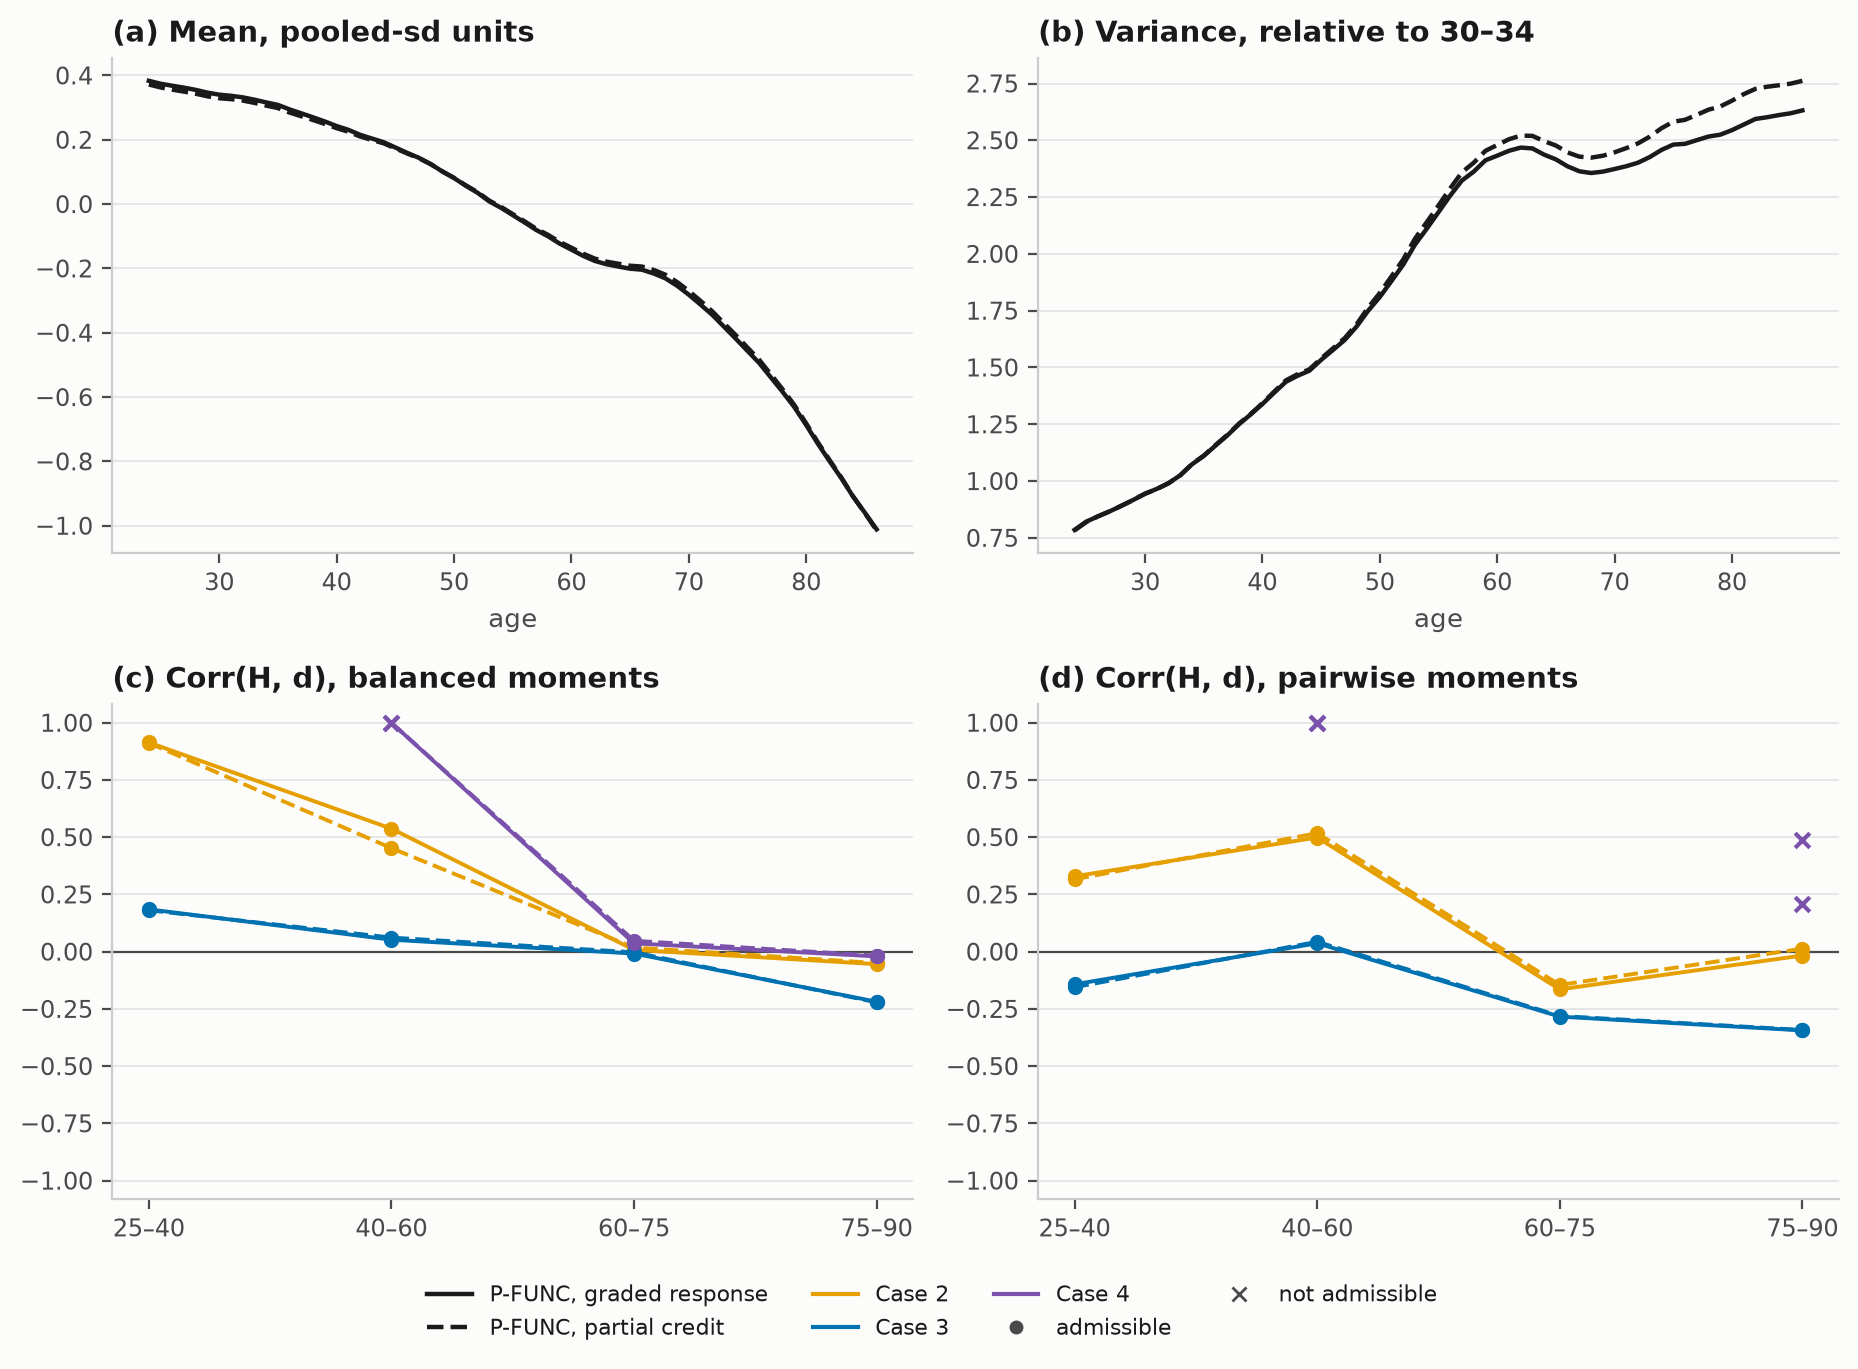
\includegraphics[width=\linewidth]{fig_lim_exhibit1_pfunc}
\caption{Exhibit 1 for P-FUNC on $h$. (a) Mean in pooled-sd units and (b)
variance relative to ages 30--34, five-year centred means; graded response
solid, partial credit dashed. (c) and (d) $\mathrm{Corr}(H,d)$ by band under
Cases 2, 3 and 4 on balanced and on pairwise moments, at the best-fitting
$\rho$. Crosses mark bands where the fit is not admissible, correlations beyond
$\pm1$ are drawn at the edge, and undefined correlations are left out.}
\label{fig:lim_ex1_pfunc}
\end{figure}

\begin{figure}[H]
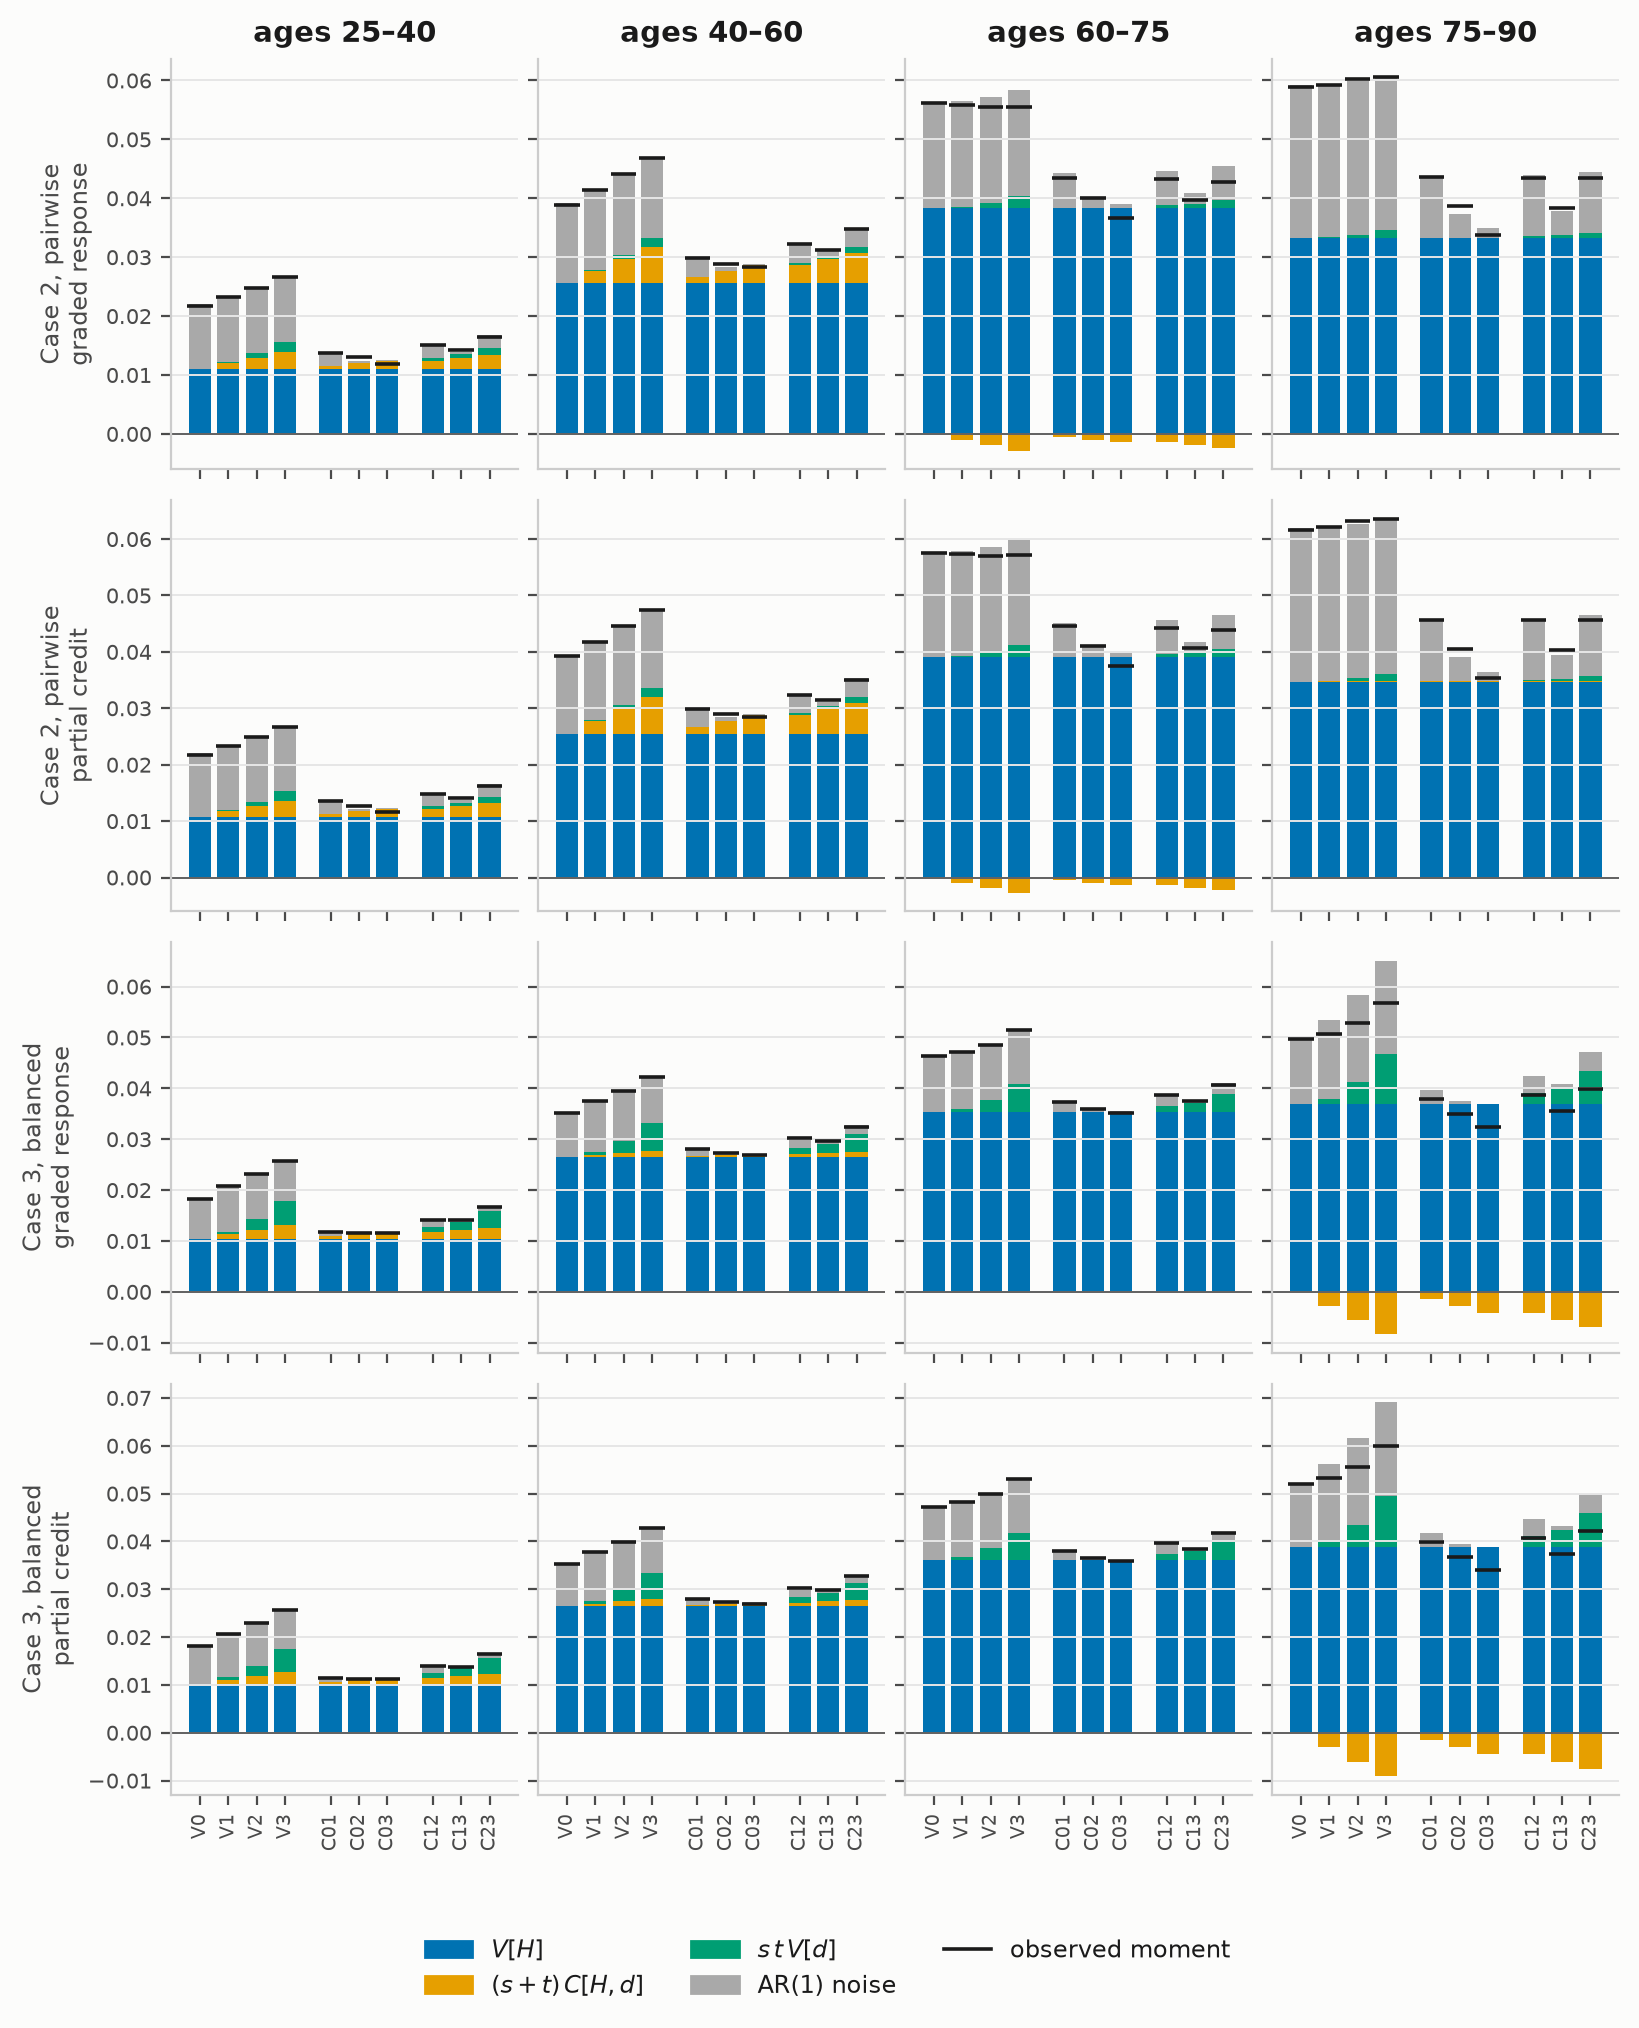
\includegraphics[width=\linewidth]{fig_lim_bars_pfunc}
\caption{Identification barcharts for P-FUNC on $h$: observed moments (black
rules) and fitted layers for the ten cells of four ages two years apart,
pooled over base ages within each band. A panel would be marked if its fit
were not admissible; none is, here or for any other bank.}
\label{fig:lim_bars_pfunc}
\end{figure}

\begin{figure}[H]
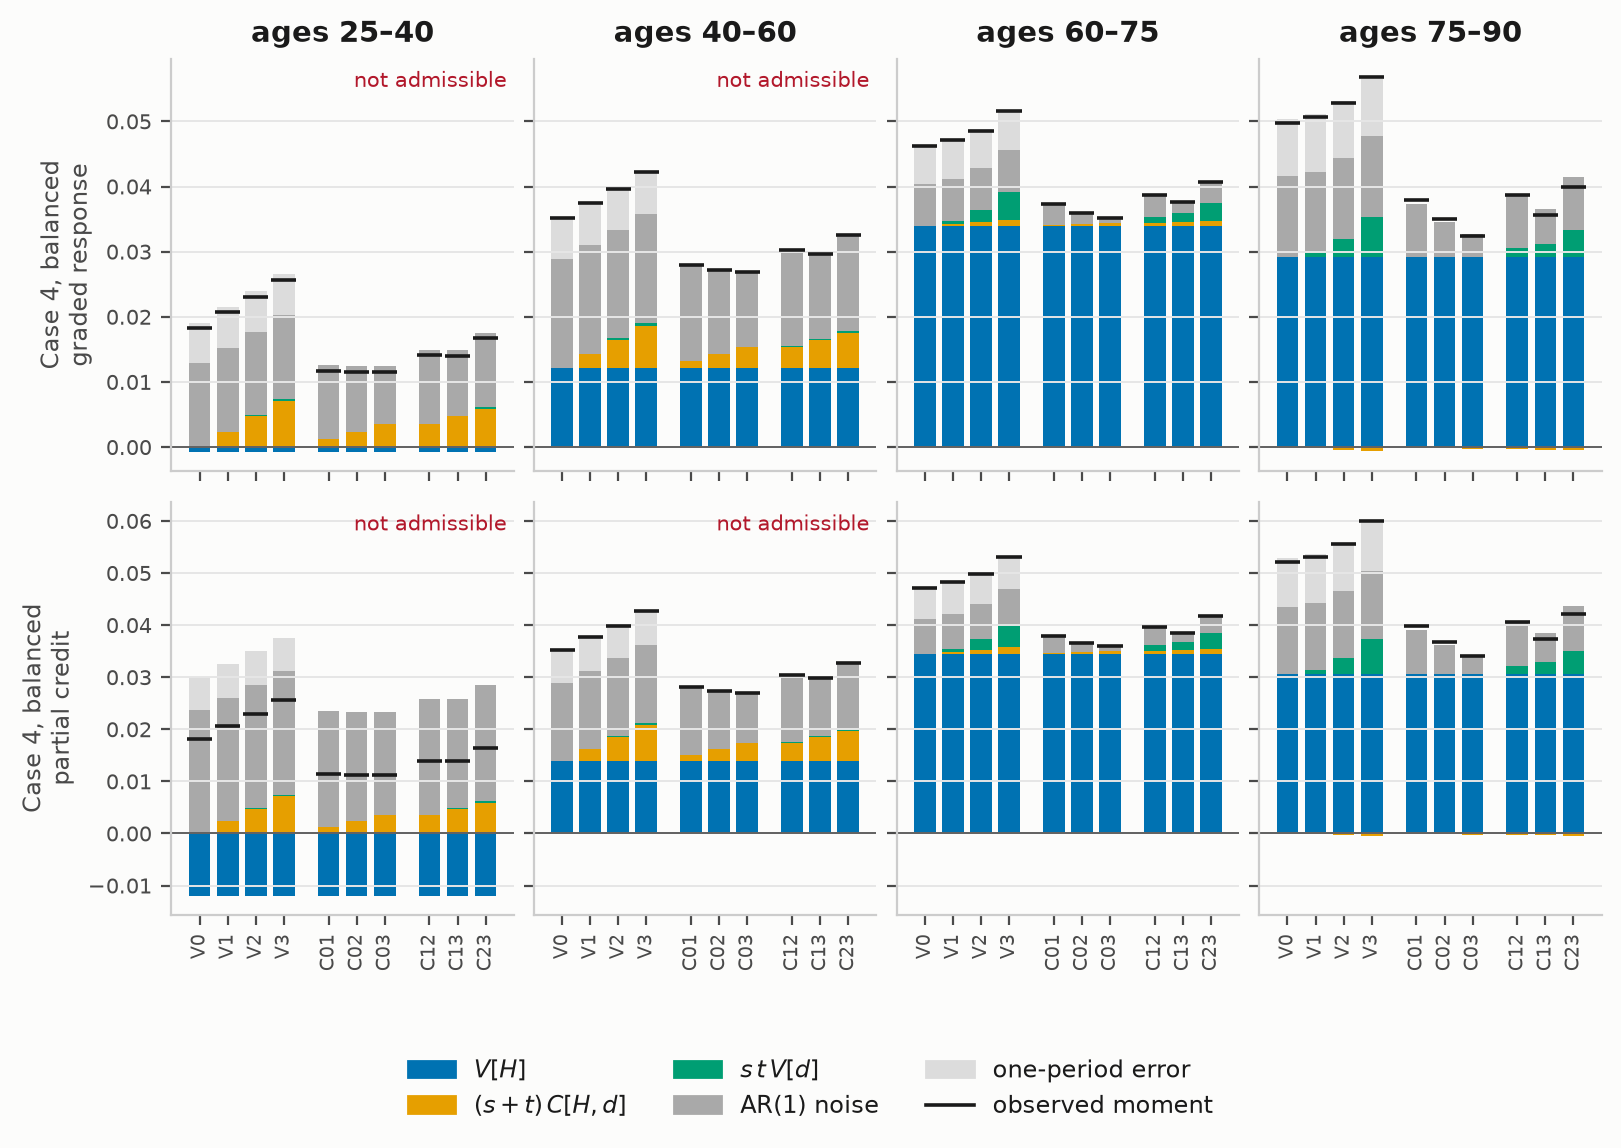
\includegraphics[width=\linewidth]{fig_lim_bars_case4_pfunc}
\caption{Case 4 barcharts for P-FUNC on $h$: balanced moments, noise split into
the AR(1) part and the one-period error, at the best-fitting $\rho$ in each band; as Figure~\ref{fig:lim_bars_pfunc} otherwise.}
\label{fig:lim_bars4_pfunc}
\end{figure}

\begin{figure}[H]
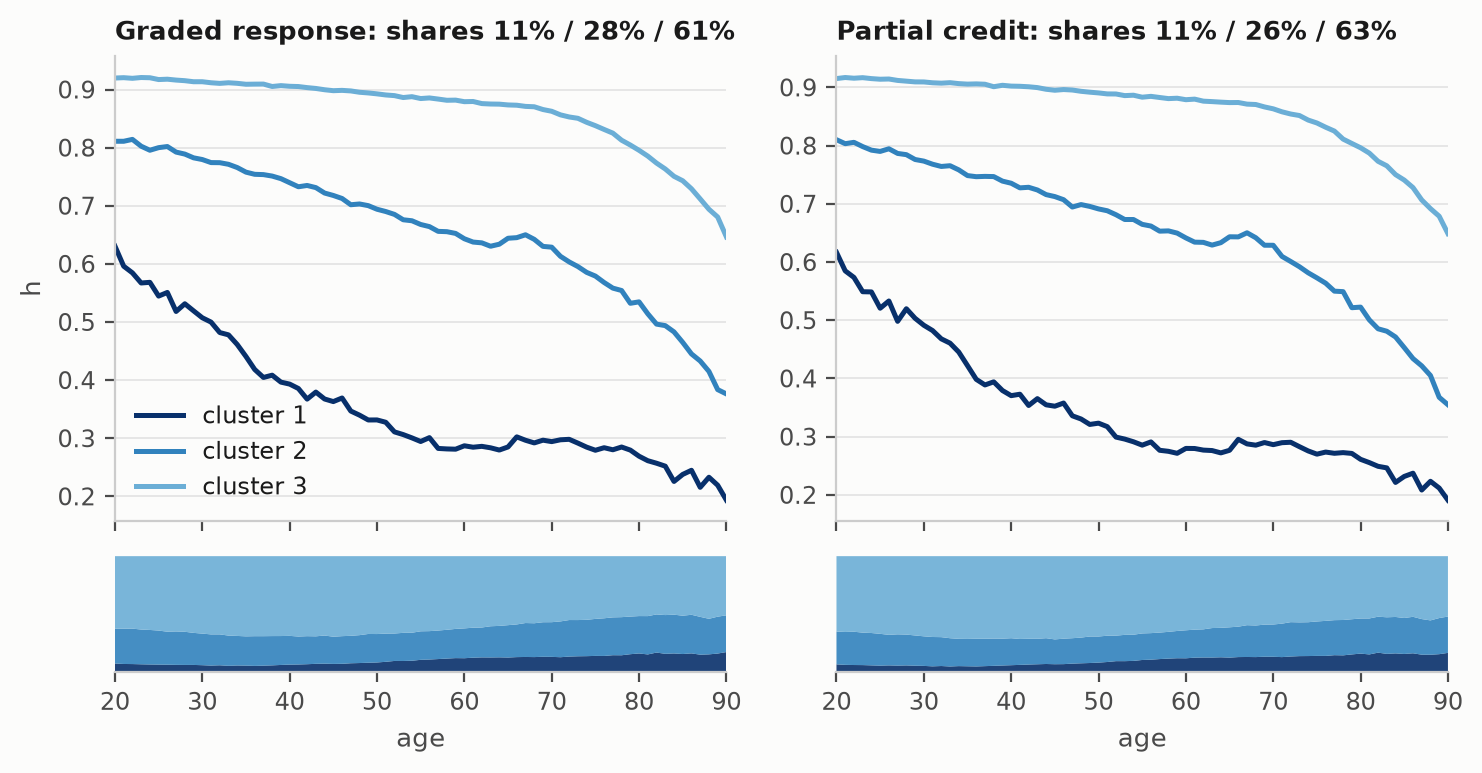
\includegraphics[width=\linewidth]{fig_lim_clusters_pfunc}
\caption{Partial K-means, $K=3$, for P-FUNC on $h$: cluster means by age where
at least 25 members are observed, and cluster shares of the observed sample
by age beneath. Graded response left, partial credit right.}
\label{fig:lim_cl_pfunc}
\end{figure}

\subsubsection{P-LIM1}
Uncapping the count alone takes the floor from 1.11\% to 0.37\%. Case 2's
oldest-band correlation turns positive, $+0.01$, and the clusters barely move:
the adjusted Rand index against P-FUNC's clusters is 0.98.

\begin{figure}[H]
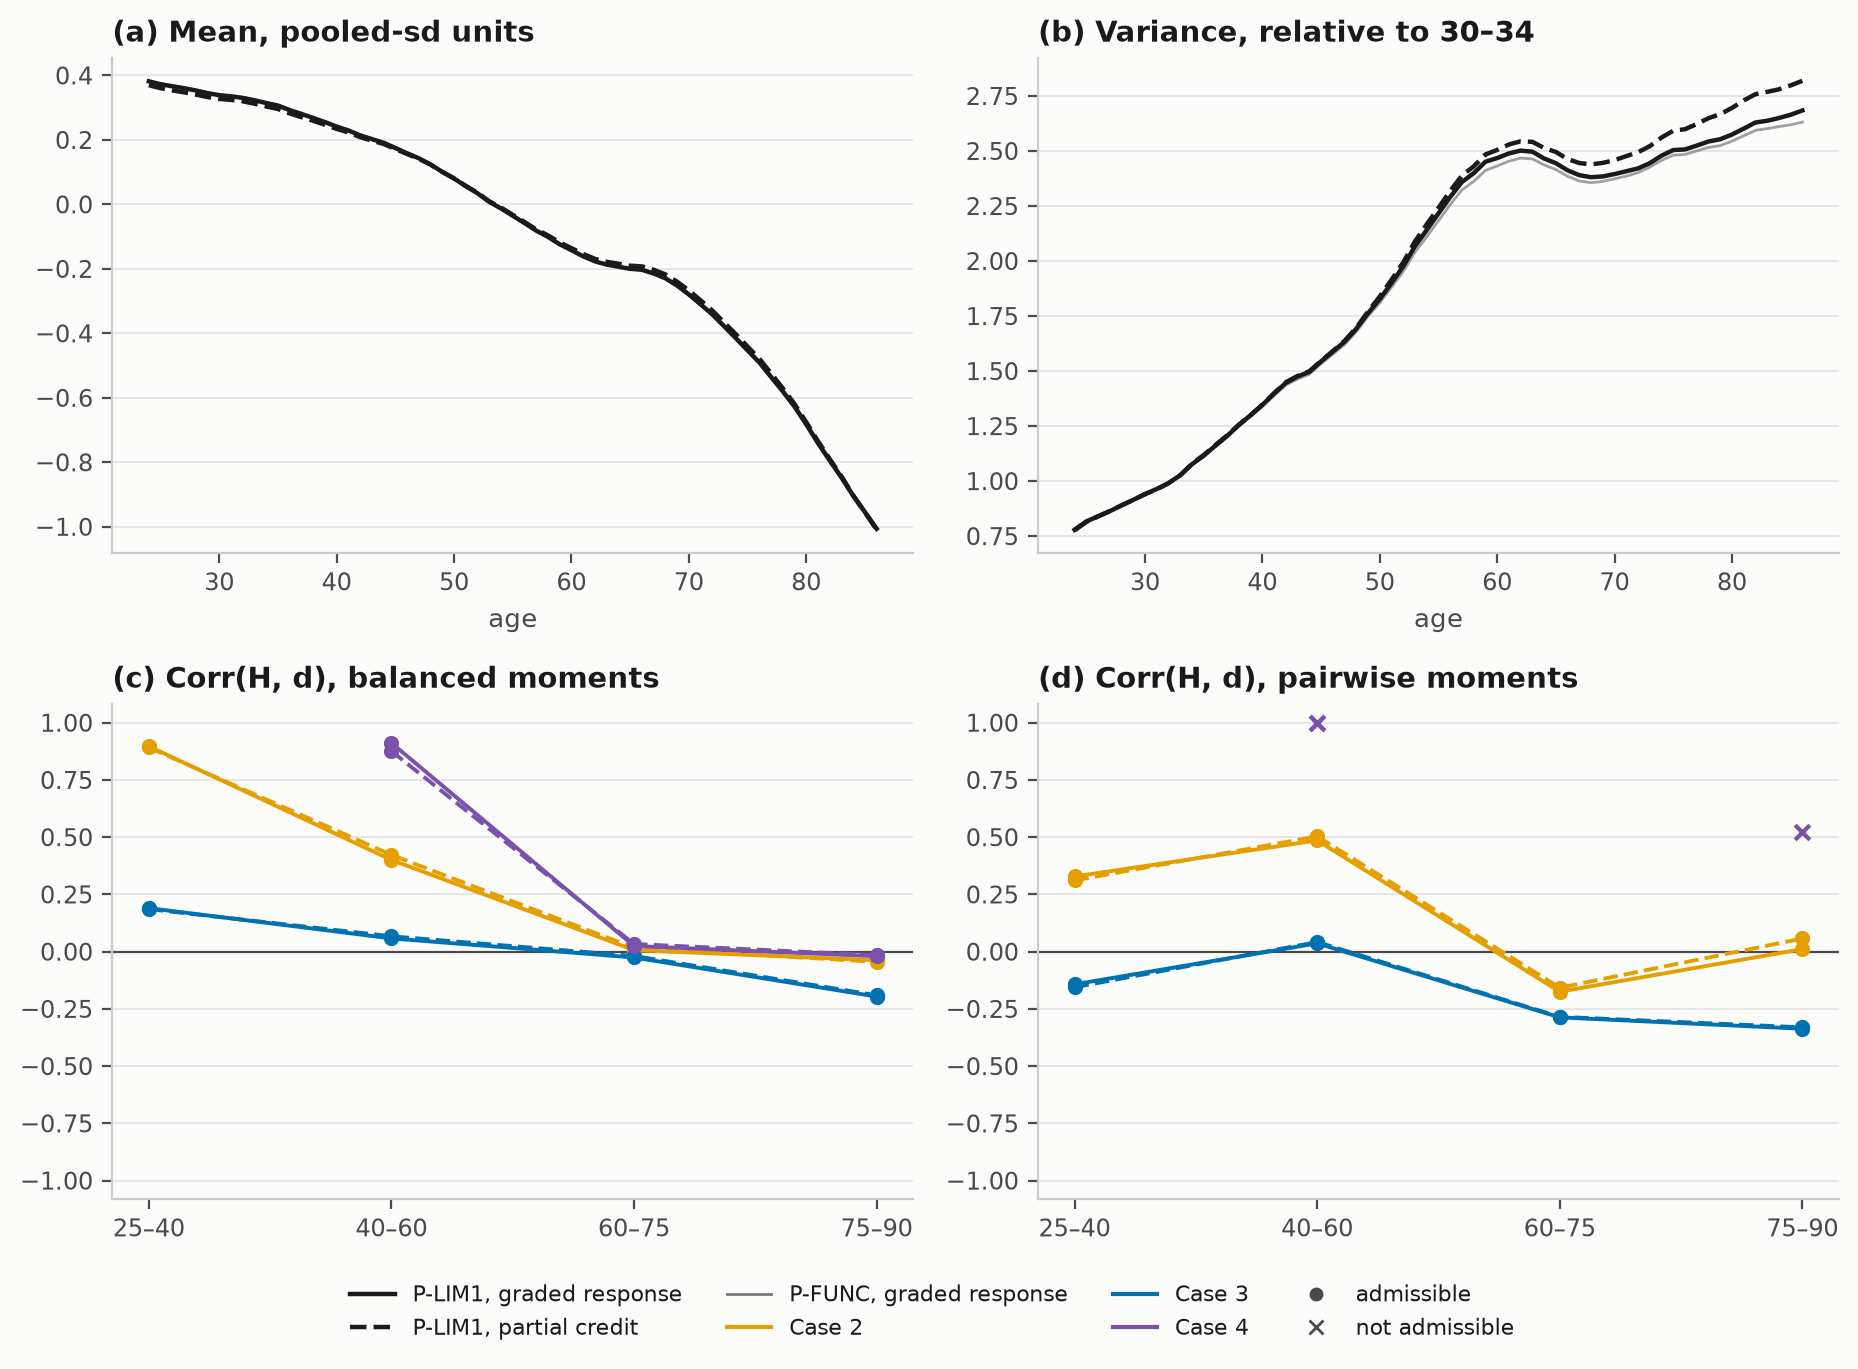
\includegraphics[width=\linewidth]{fig_lim_exhibit1_plim1}
\caption{Exhibit 1 for P-LIM1 on $h$, as Figure~\ref{fig:lim_ex1_pfunc}; the
grey lines in (a) and (b) are P-FUNC under the graded-response model.}
\label{fig:lim_ex1_plim1}
\end{figure}

\begin{figure}[H]
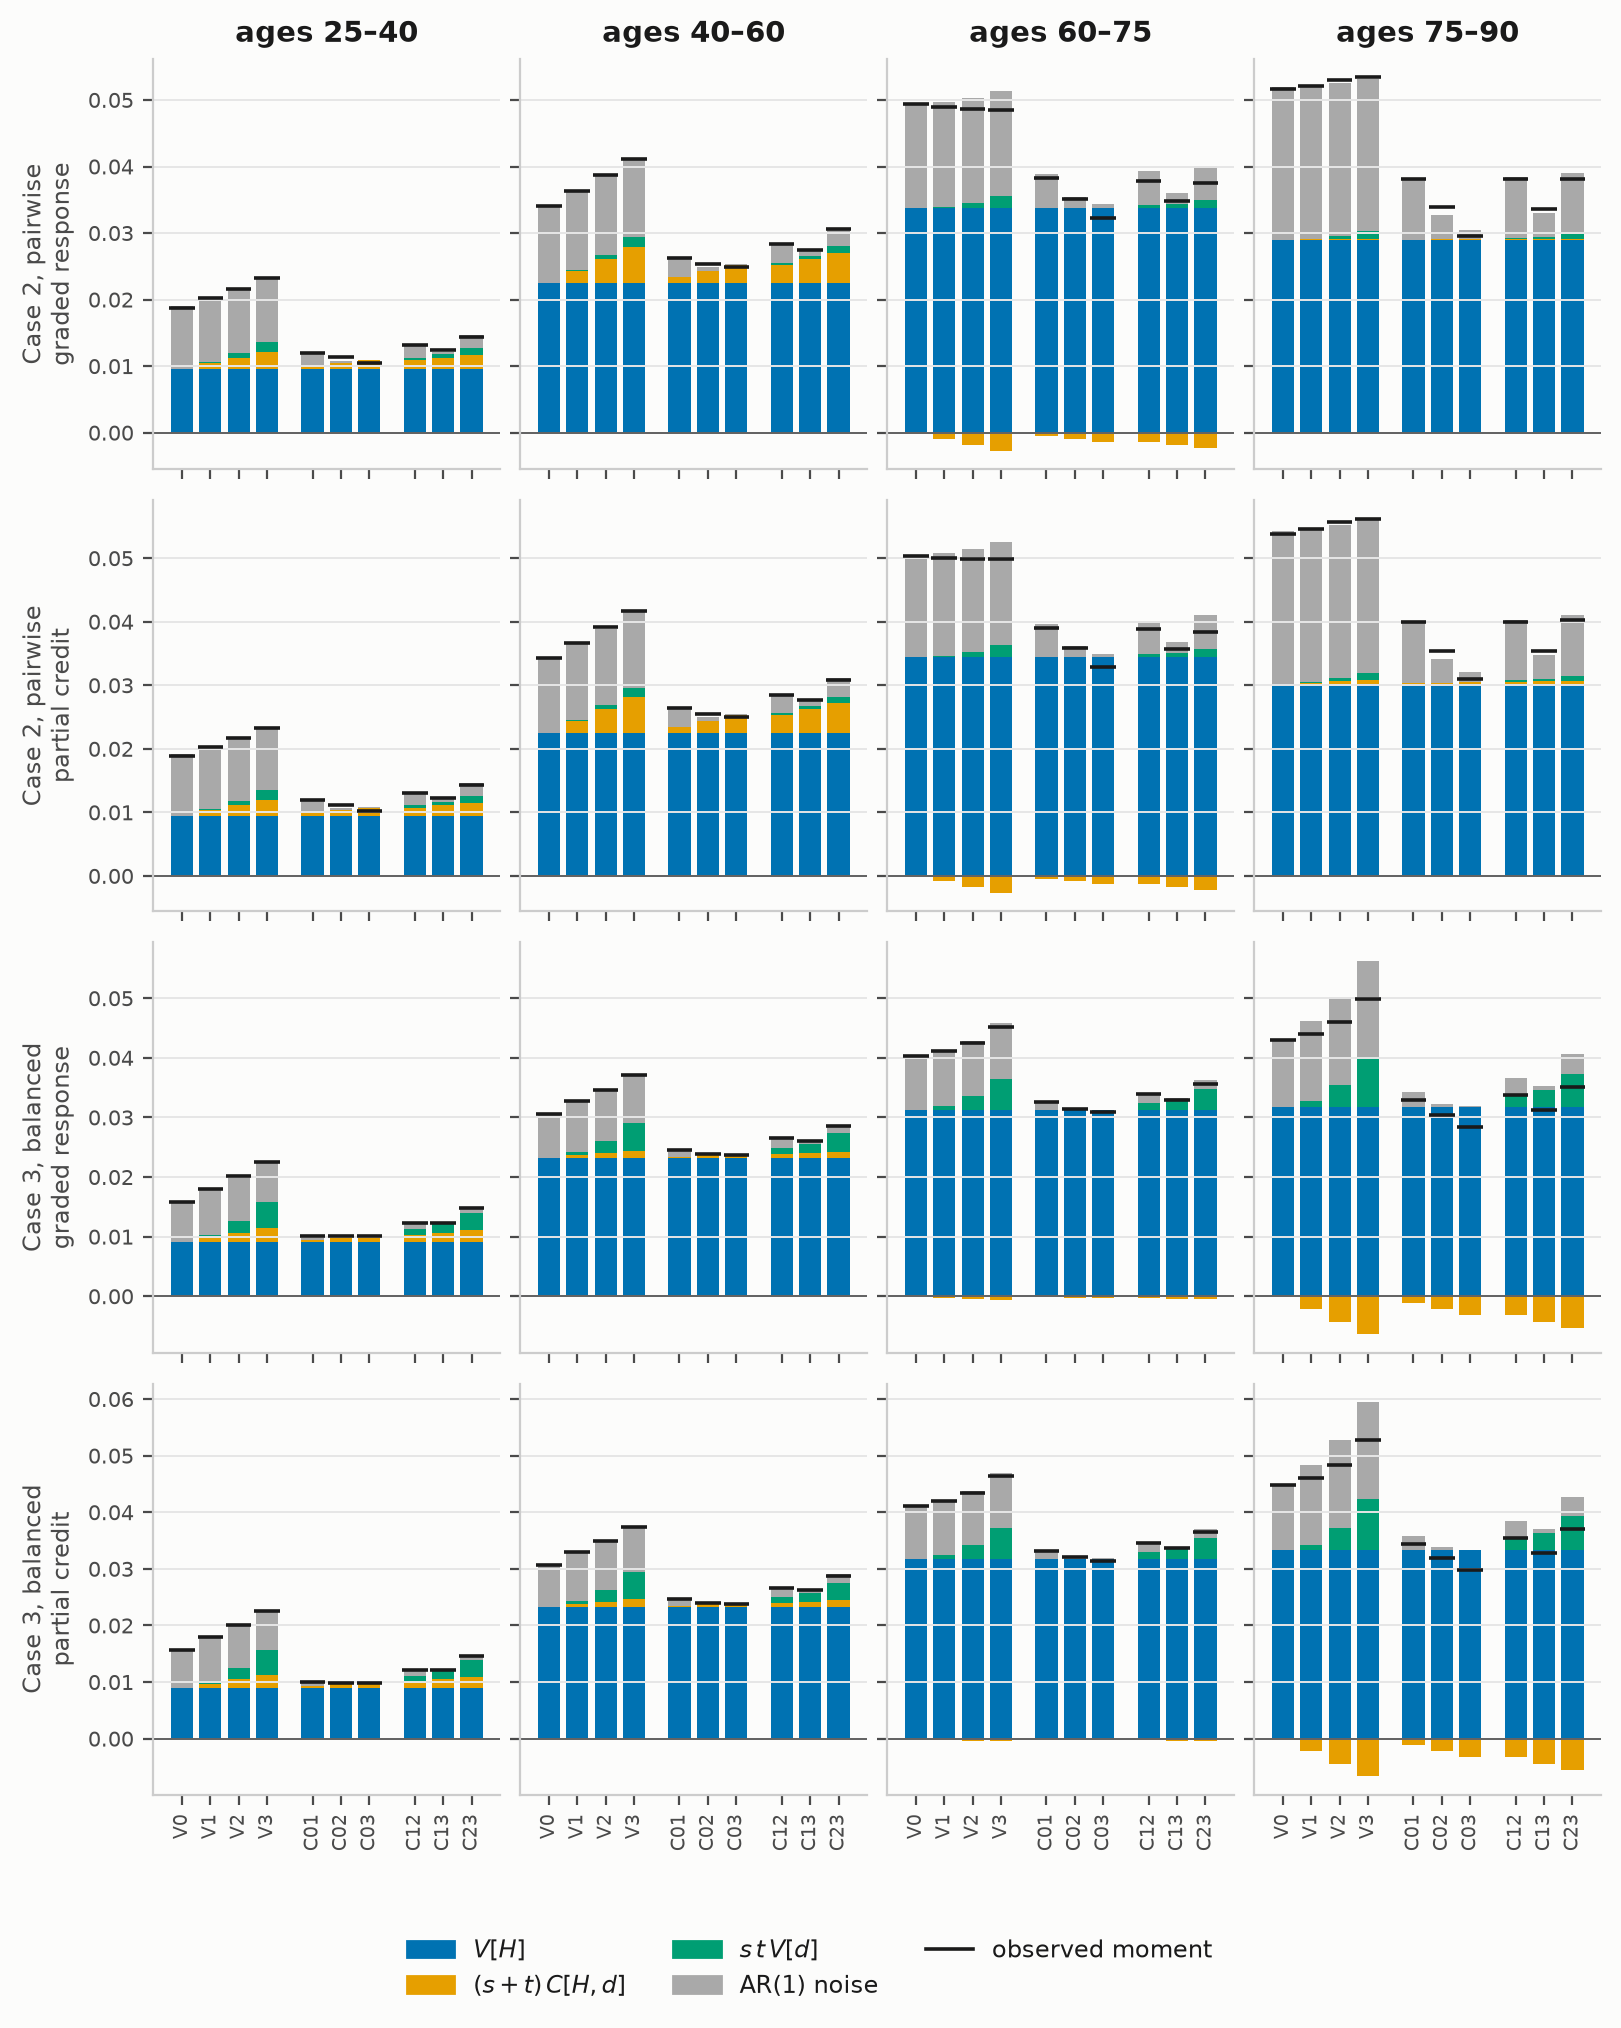
\includegraphics[width=\linewidth]{fig_lim_bars_plim1}
\caption{Identification barcharts for P-LIM1 on $h$, as
Figure~\ref{fig:lim_bars_pfunc}.}
\label{fig:lim_bars_plim1}
\end{figure}

\begin{figure}[H]
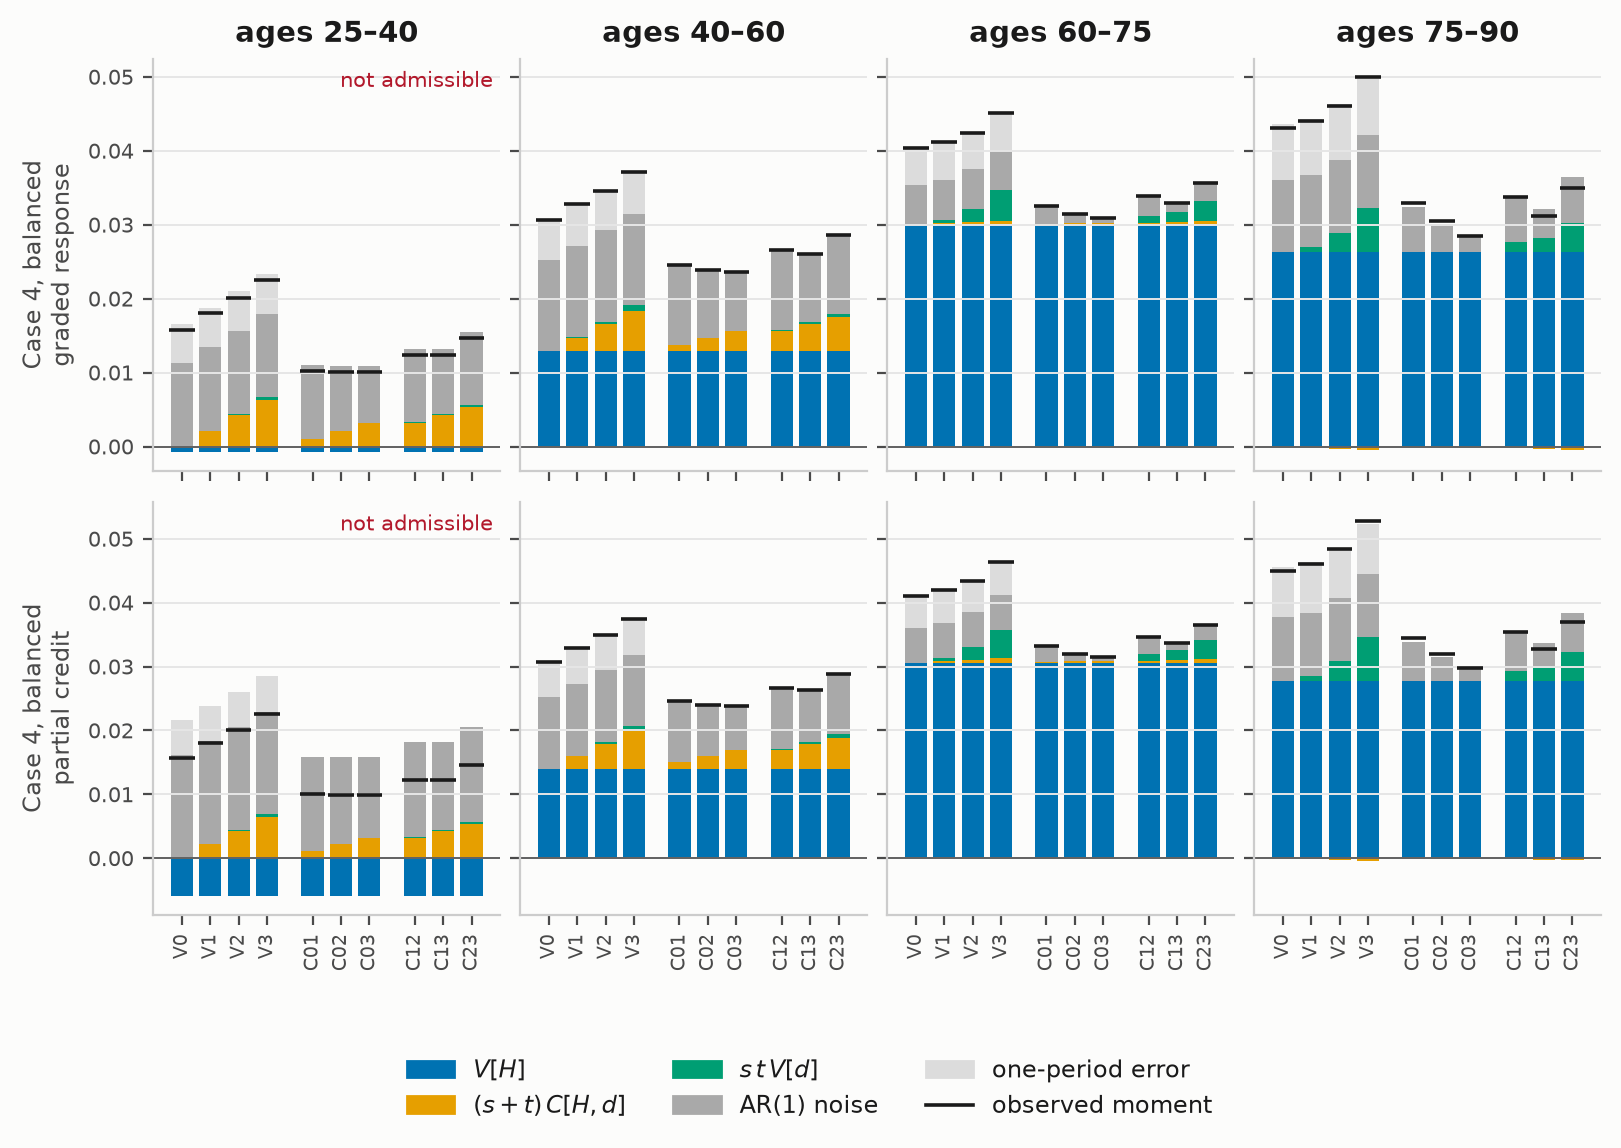
\includegraphics[width=\linewidth]{fig_lim_bars_case4_plim1}
\caption{Case 4 barcharts for P-LIM1 on $h$: balanced moments, noise split into
the AR(1) part and the one-period error.}
\label{fig:lim_bars4_plim1}
\end{figure}

\begin{figure}[H]
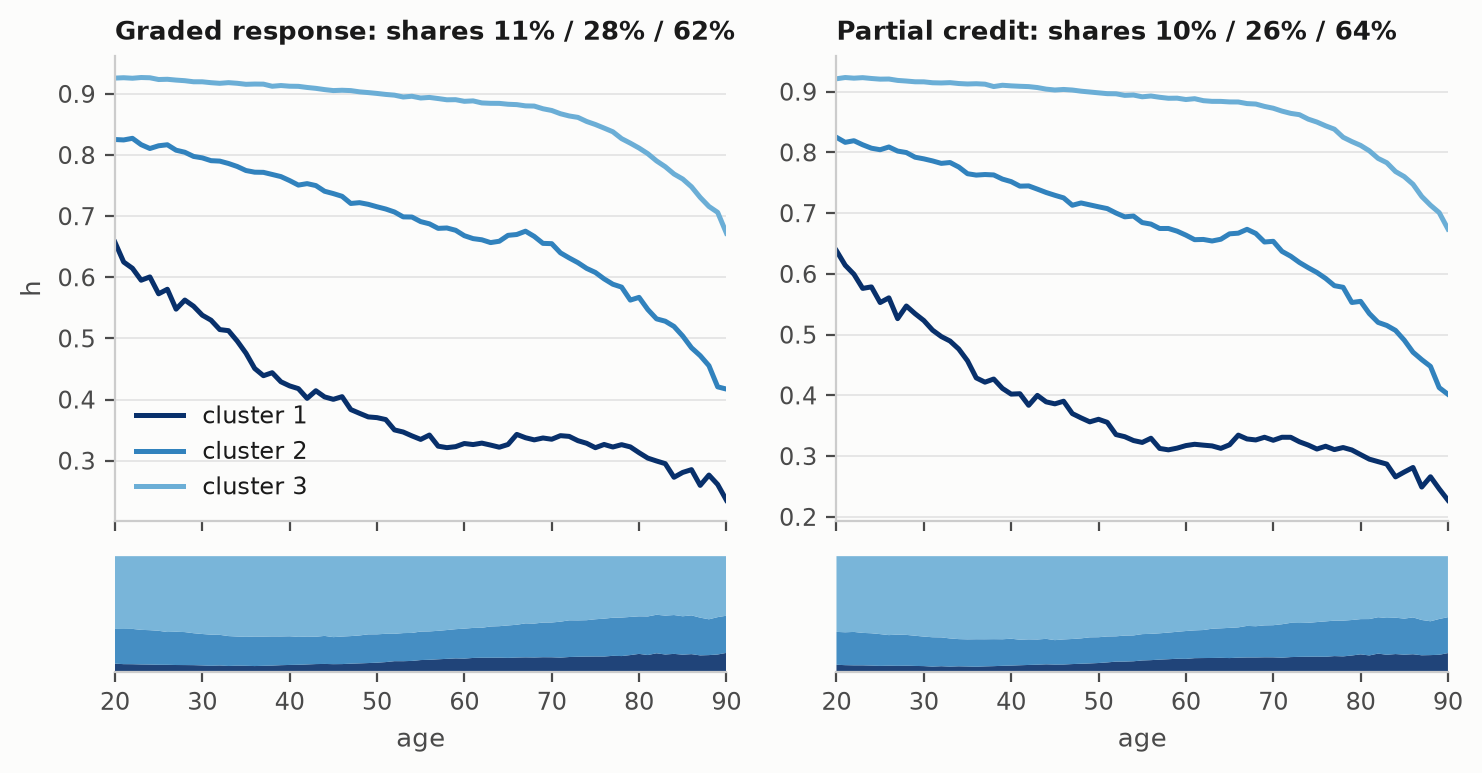
\includegraphics[width=\linewidth]{fig_lim_clusters_plim1}
\caption{Partial K-means, $K=3$, for P-LIM1 on $h$, as
Figure~\ref{fig:lim_cl_pfunc}.}
\label{fig:lim_cl_plim1}
\end{figure}

\subsubsection{P-LIM}
Sensory and continence take the floor to 0.10\%, with 4\% of observed weight.
The two counts carry the largest residual dependence of any bank, $+0.083$.
Case 2's oldest-band correlation is $+0.04$, or $+0.09$ under partial credit.

\begin{figure}[H]
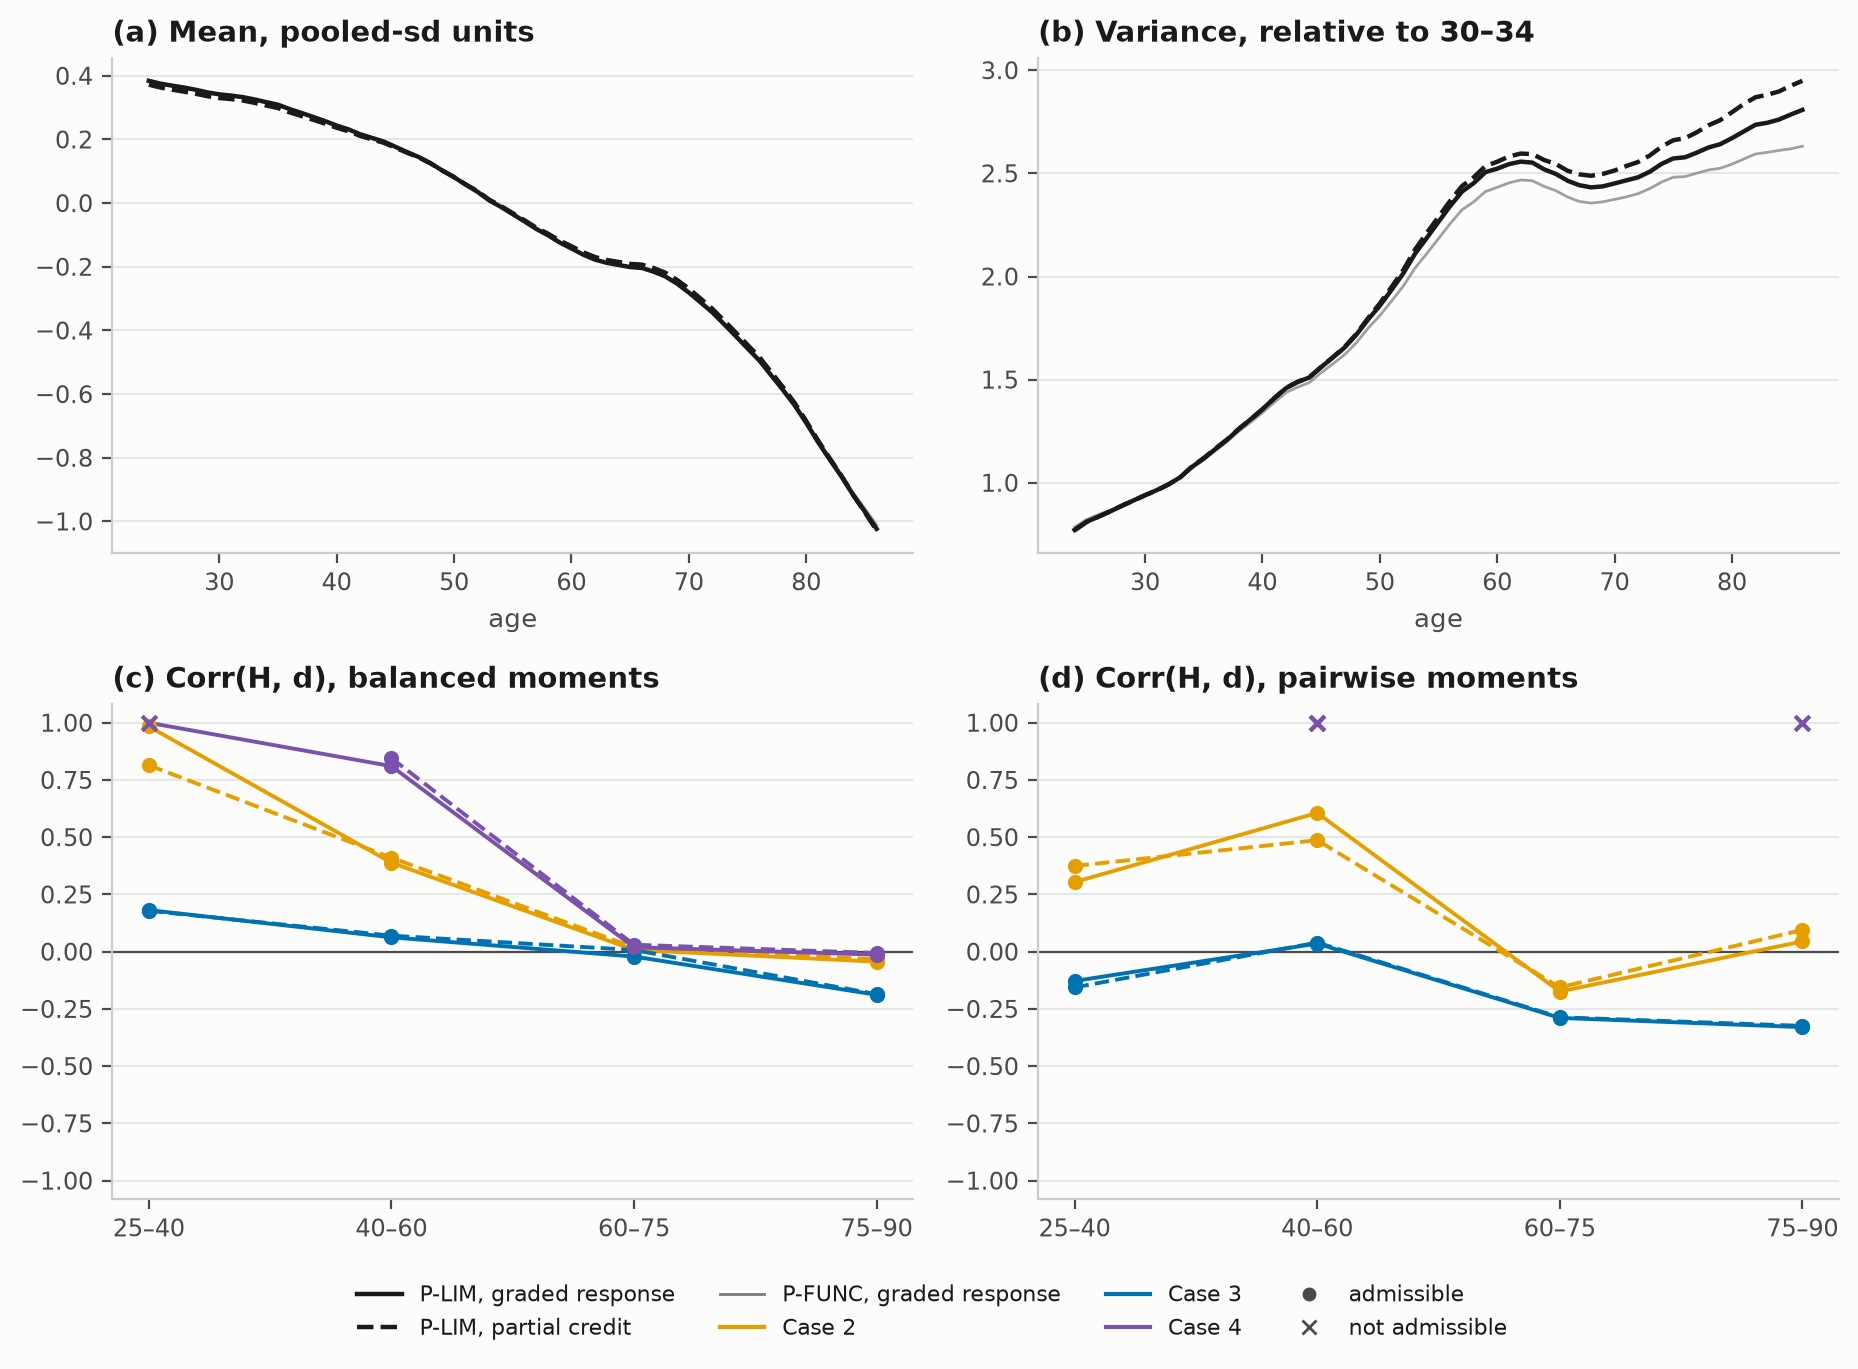
\includegraphics[width=\linewidth]{fig_lim_exhibit1_plim}
\caption{Exhibit 1 for P-LIM on $h$, as Figure~\ref{fig:lim_ex1_plim1}.}
\label{fig:lim_ex1_plim}
\end{figure}

\begin{figure}[H]
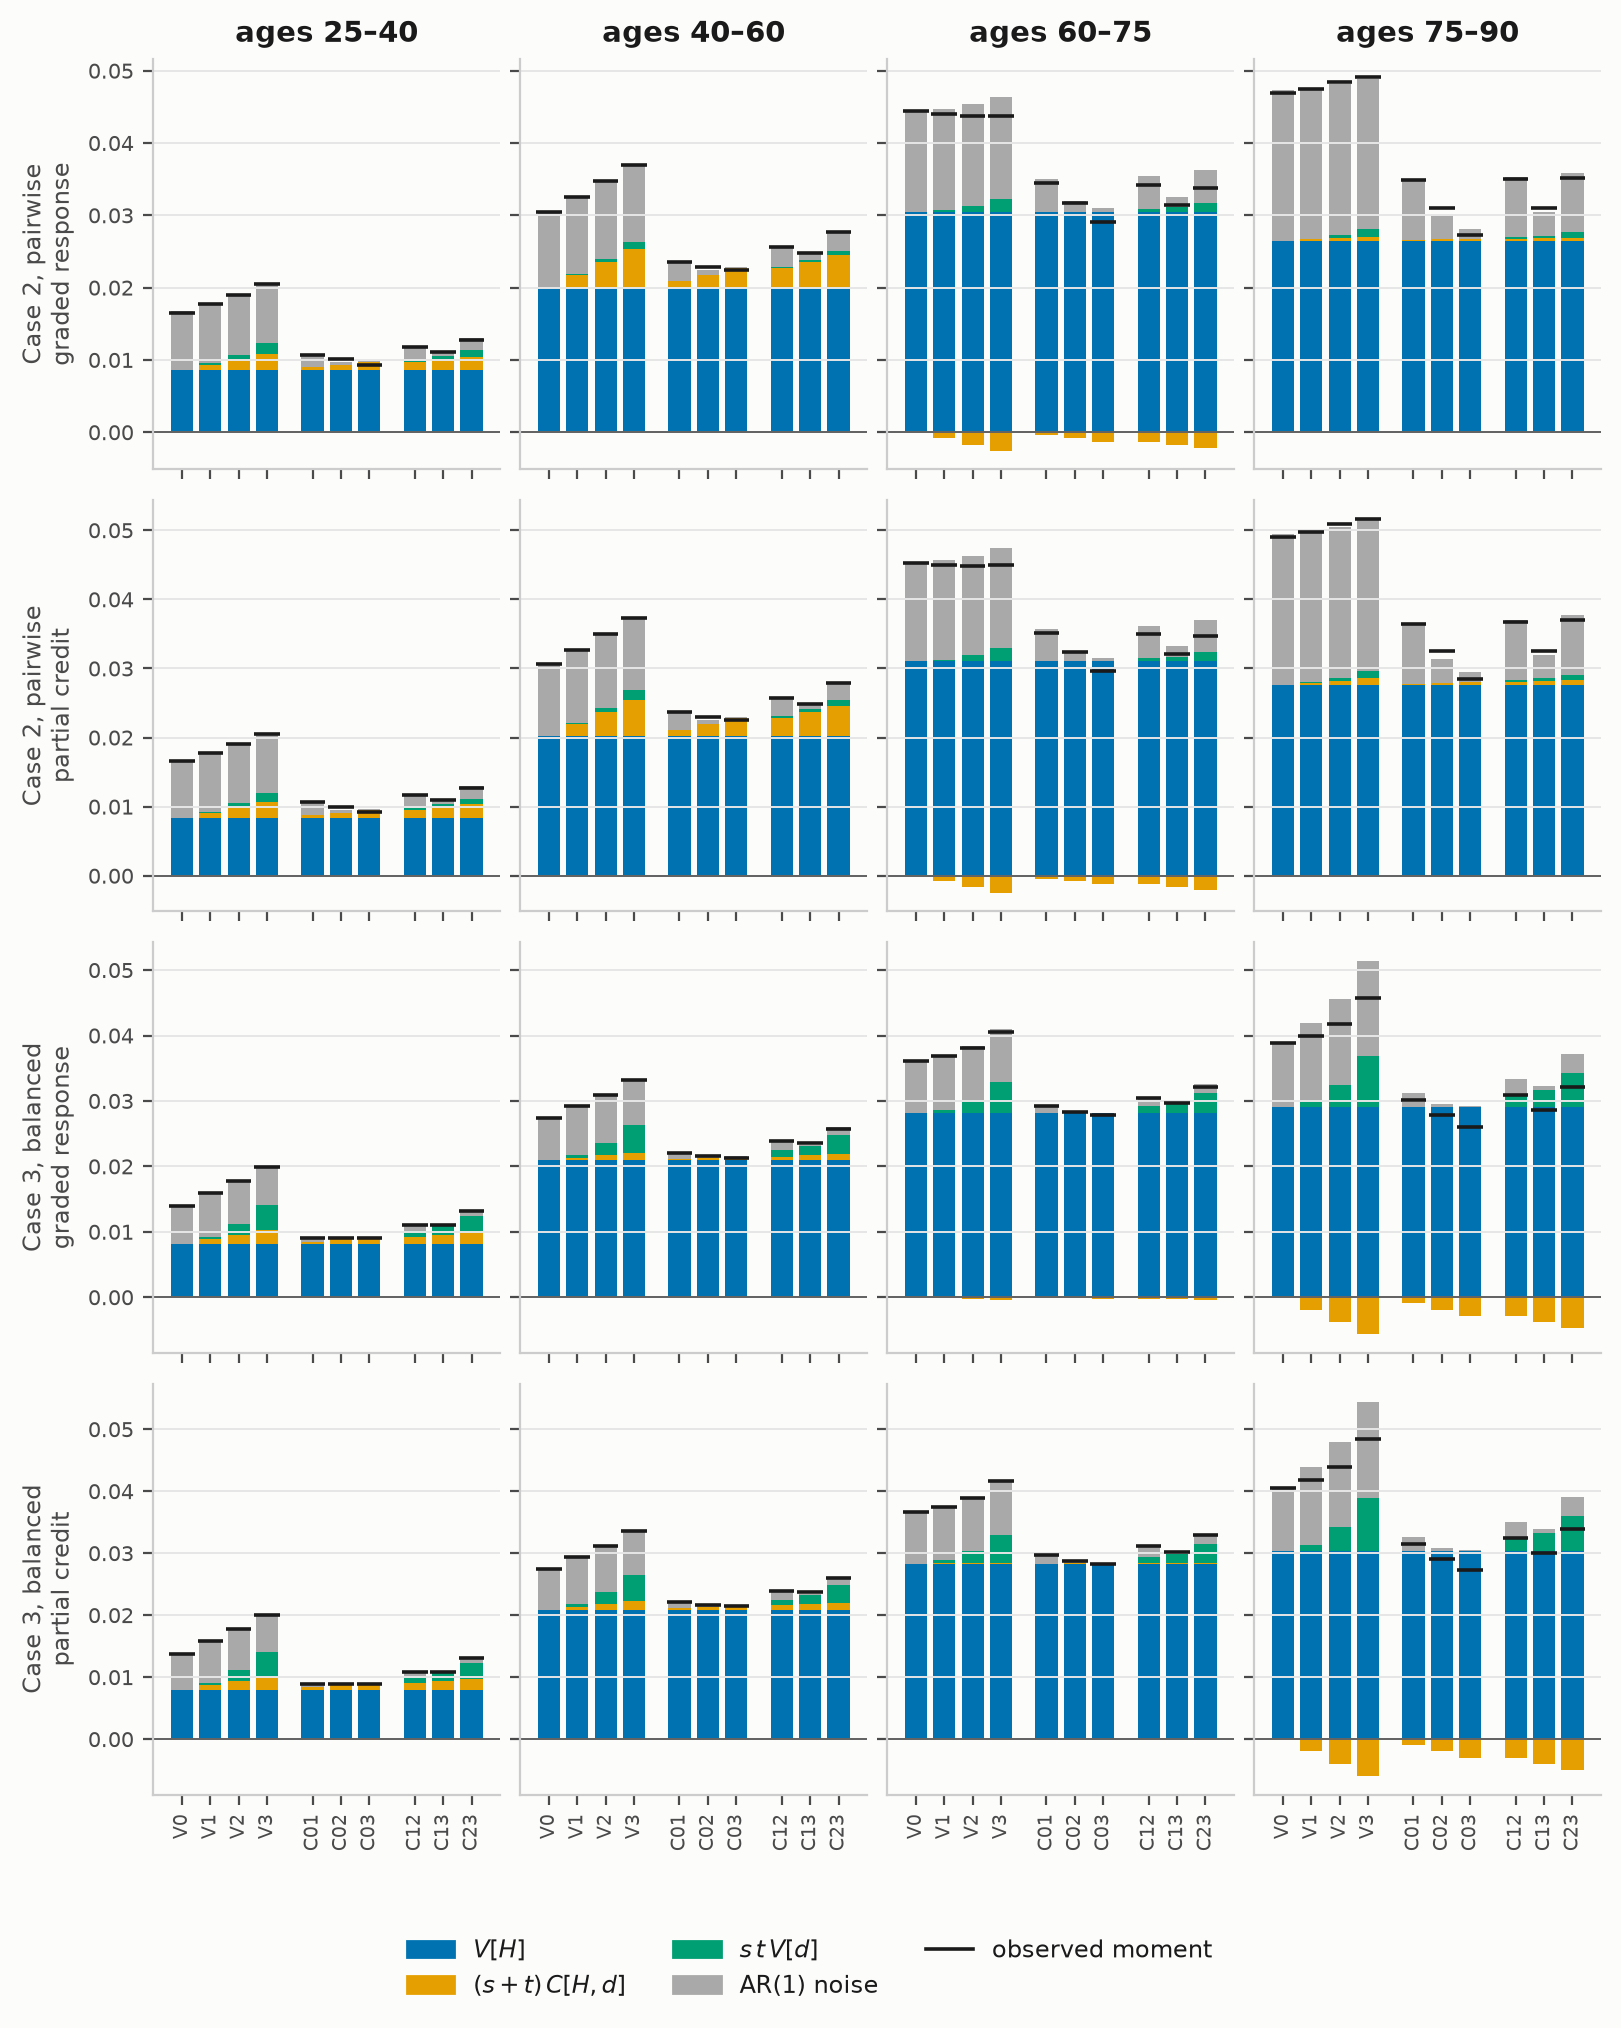
\includegraphics[width=\linewidth]{fig_lim_bars_plim}
\caption{Identification barcharts for P-LIM on $h$, as
Figure~\ref{fig:lim_bars_pfunc}.}
\label{fig:lim_bars_plim}
\end{figure}

\begin{figure}[H]
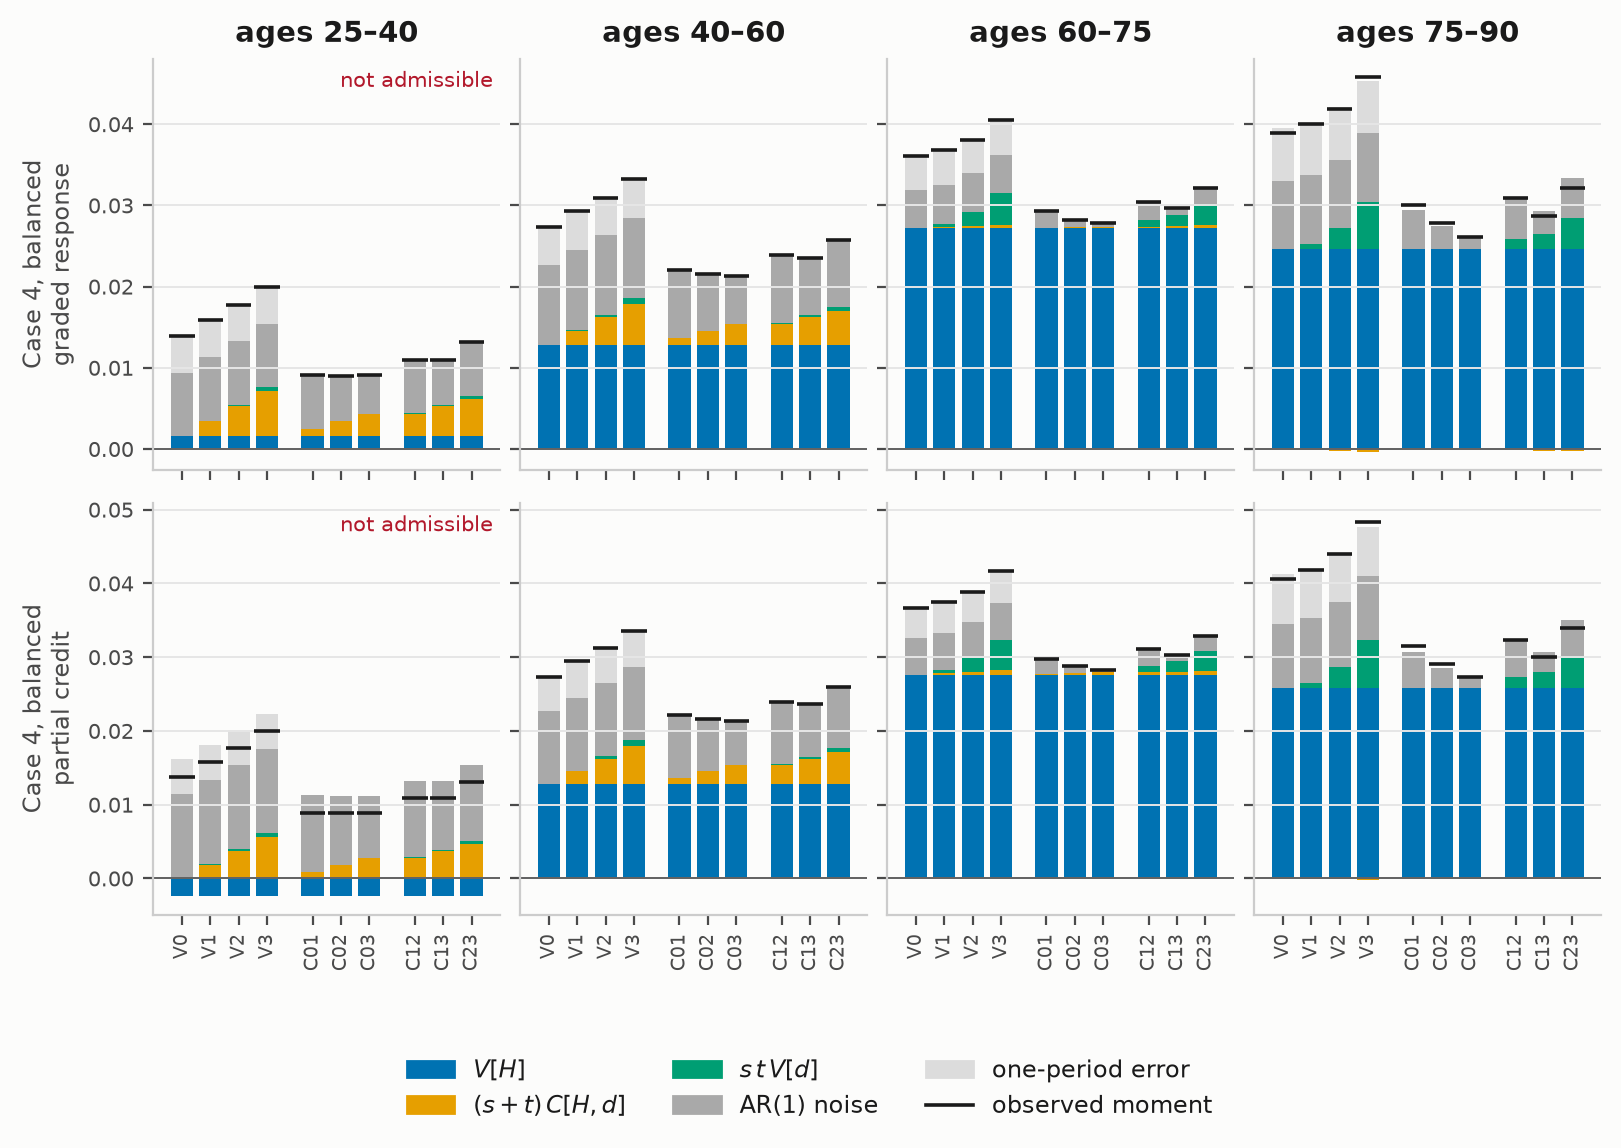
\includegraphics[width=\linewidth]{fig_lim_bars_case4_plim}
\caption{Case 4 barcharts for P-LIM on $h$: balanced moments, noise split into
the AR(1) part and the one-period error.}
\label{fig:lim_bars4_plim}
\end{figure}

\begin{figure}[H]
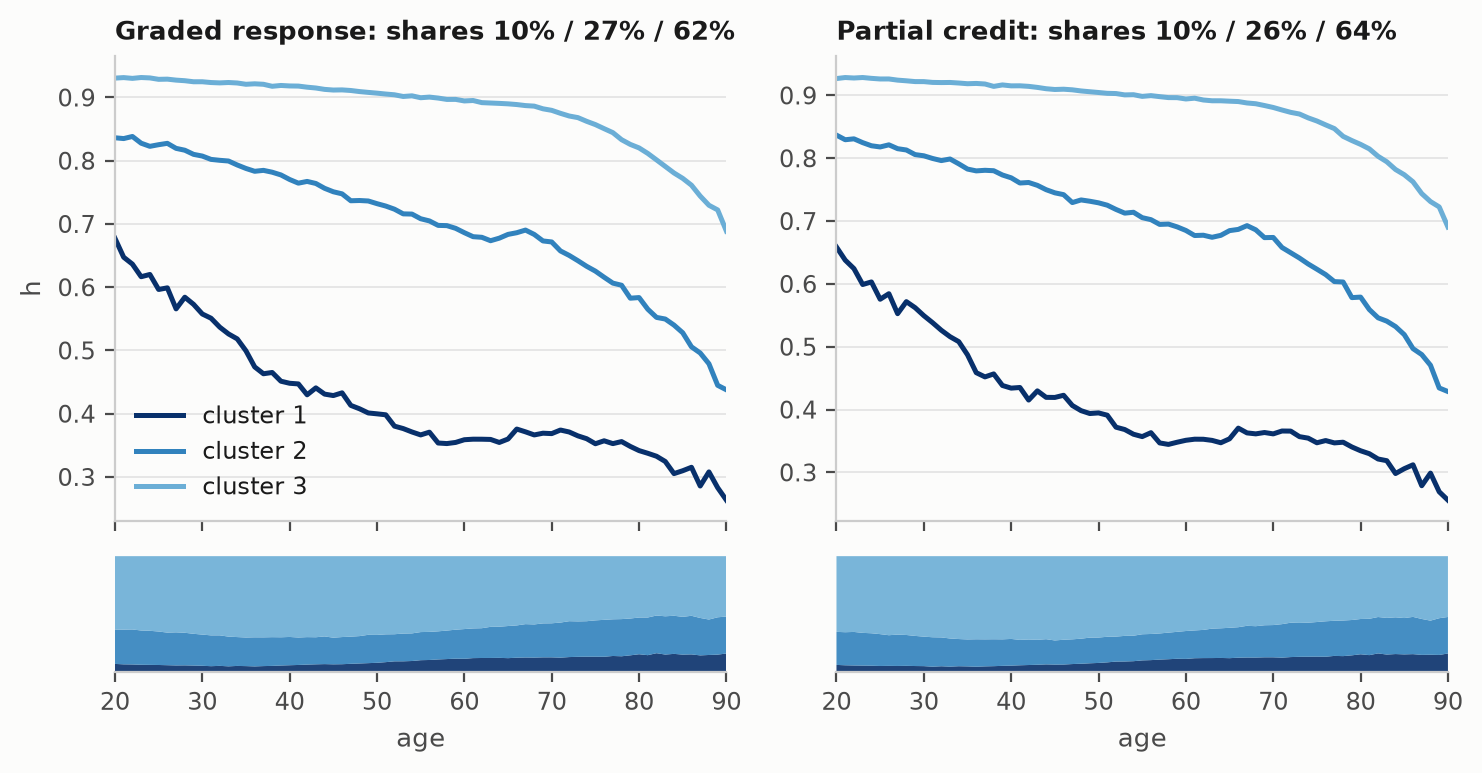
\includegraphics[width=\linewidth]{fig_lim_clusters_plim}
\caption{Partial K-means, $K=3$, for P-LIM on $h$, as
Figure~\ref{fig:lim_cl_pfunc}.}
\label{fig:lim_cl_plim}
\end{figure}

\subsubsection{P-LIM4}
The finest split. Mobility and lifting get 22\% of latent weight but 15\% of
observed weight, and continence and hearing and sight get 3\% or less of
observed weight. This bank has the weakest capped cost $t$, 10.6
under the graded-response model and 8.4 under partial credit, and the most
variance growth, 1.13.

\begin{figure}[H]
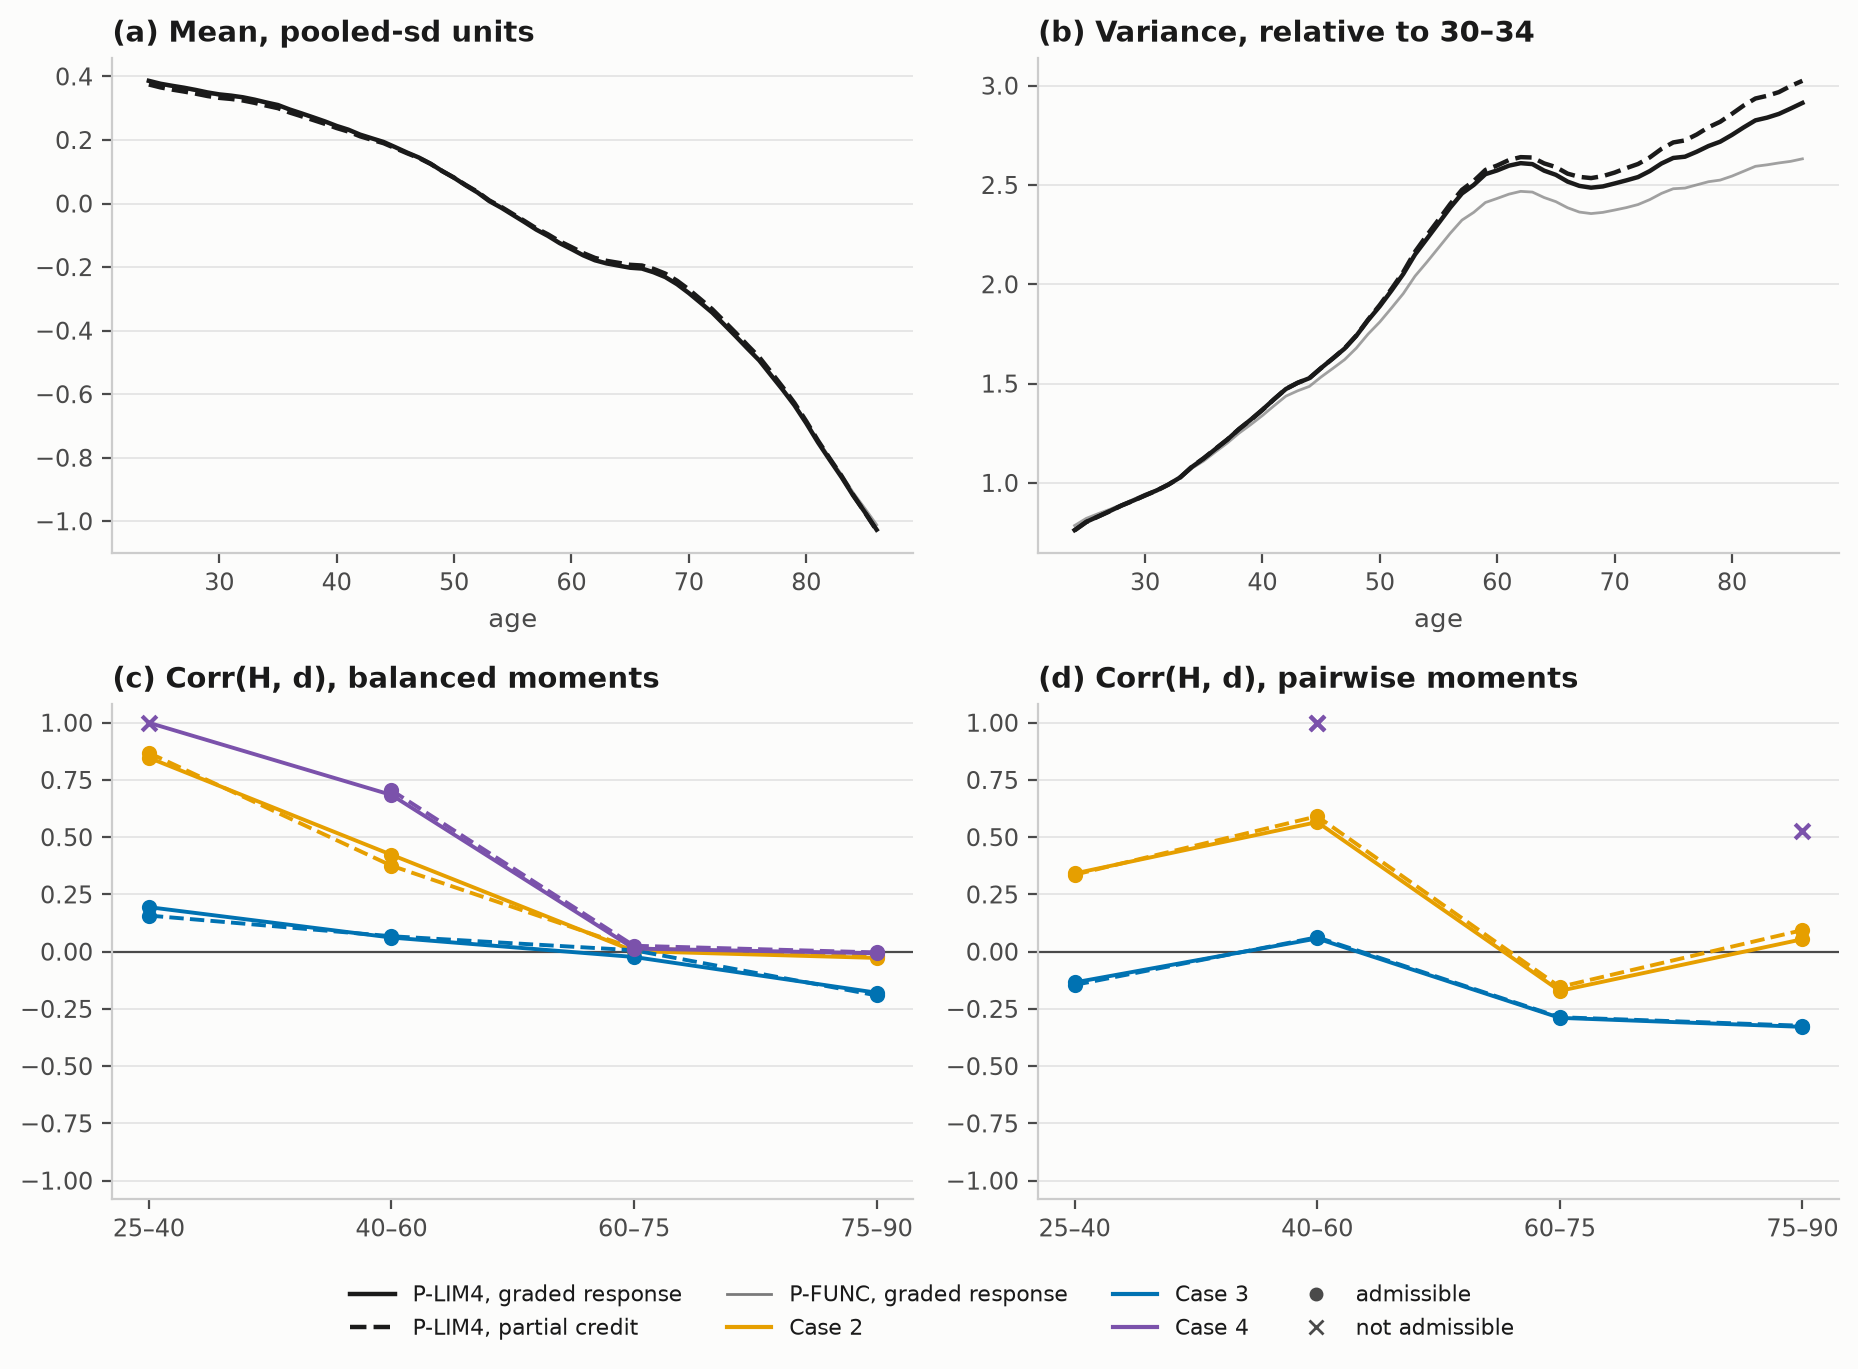
\includegraphics[width=\linewidth]{fig_lim_exhibit1_plim4}
\caption{Exhibit 1 for P-LIM4 on $h$, as Figure~\ref{fig:lim_ex1_plim1}.}
\label{fig:lim_ex1_plim4}
\end{figure}

\begin{figure}[H]
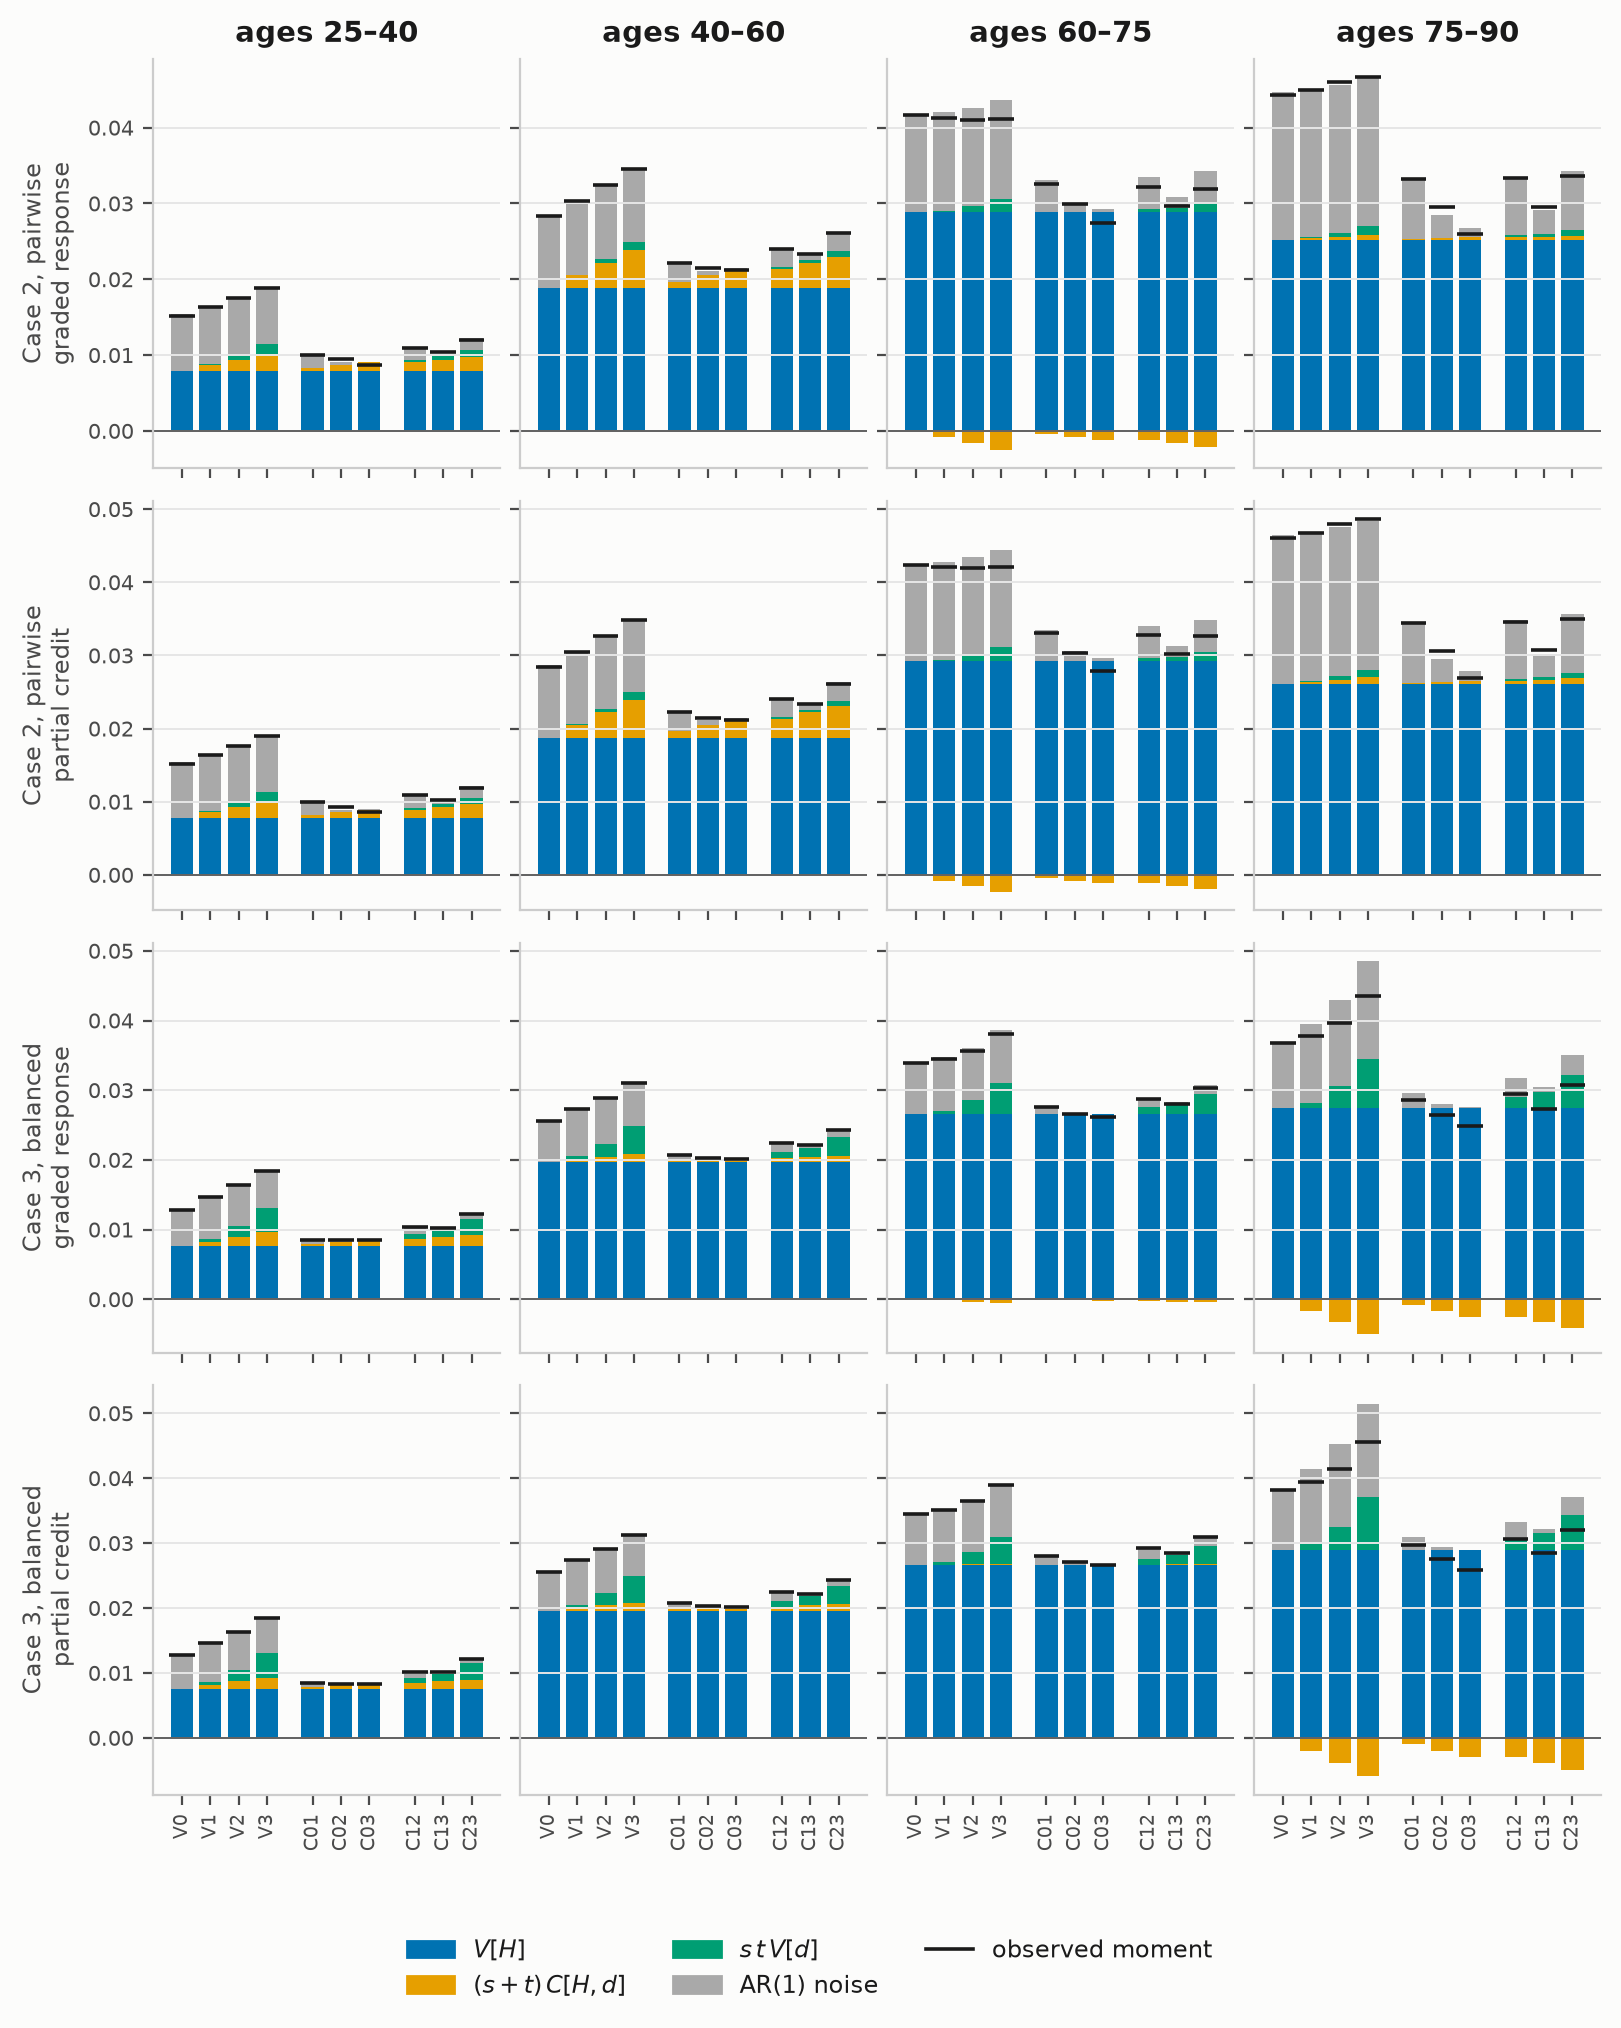
\includegraphics[width=\linewidth]{fig_lim_bars_plim4}
\caption{Identification barcharts for P-LIM4 on $h$, as
Figure~\ref{fig:lim_bars_pfunc}.}
\label{fig:lim_bars_plim4}
\end{figure}

\begin{figure}[H]
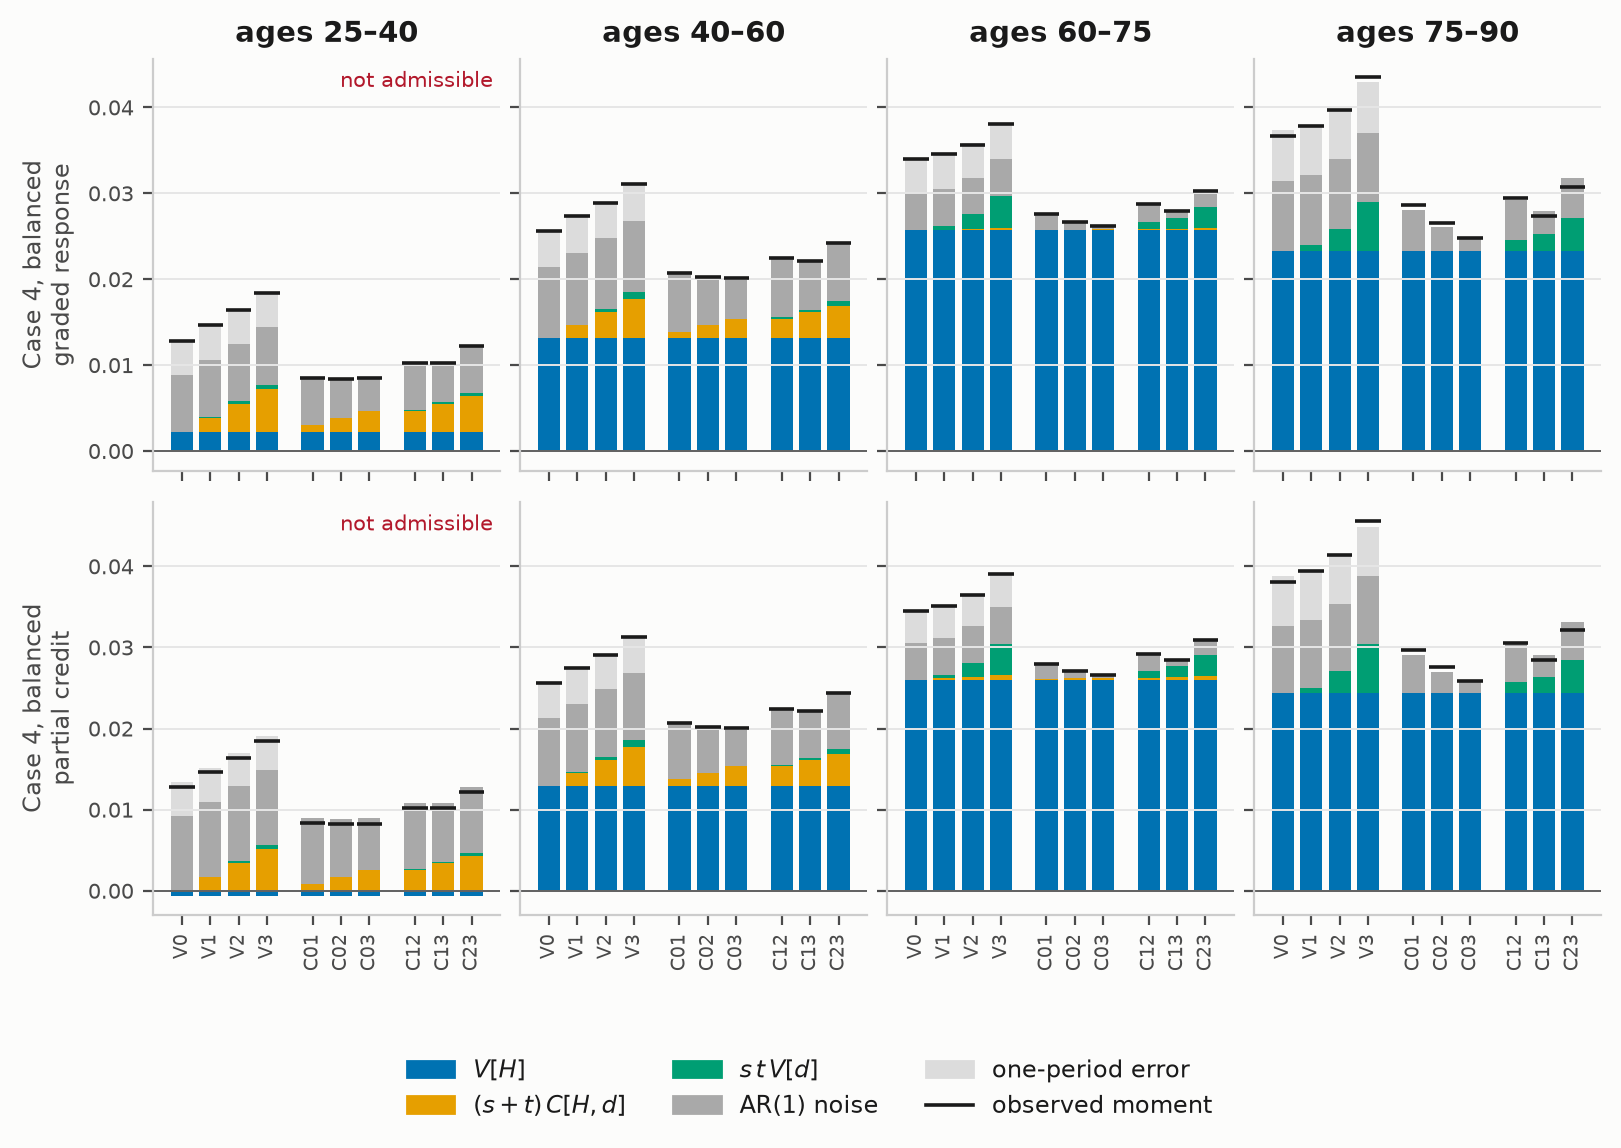
\includegraphics[width=\linewidth]{fig_lim_bars_case4_plim4}
\caption{Case 4 barcharts for P-LIM4 on $h$: balanced moments, noise split into
the AR(1) part and the one-period error.}
\label{fig:lim_bars4_plim4}
\end{figure}

\begin{figure}[H]
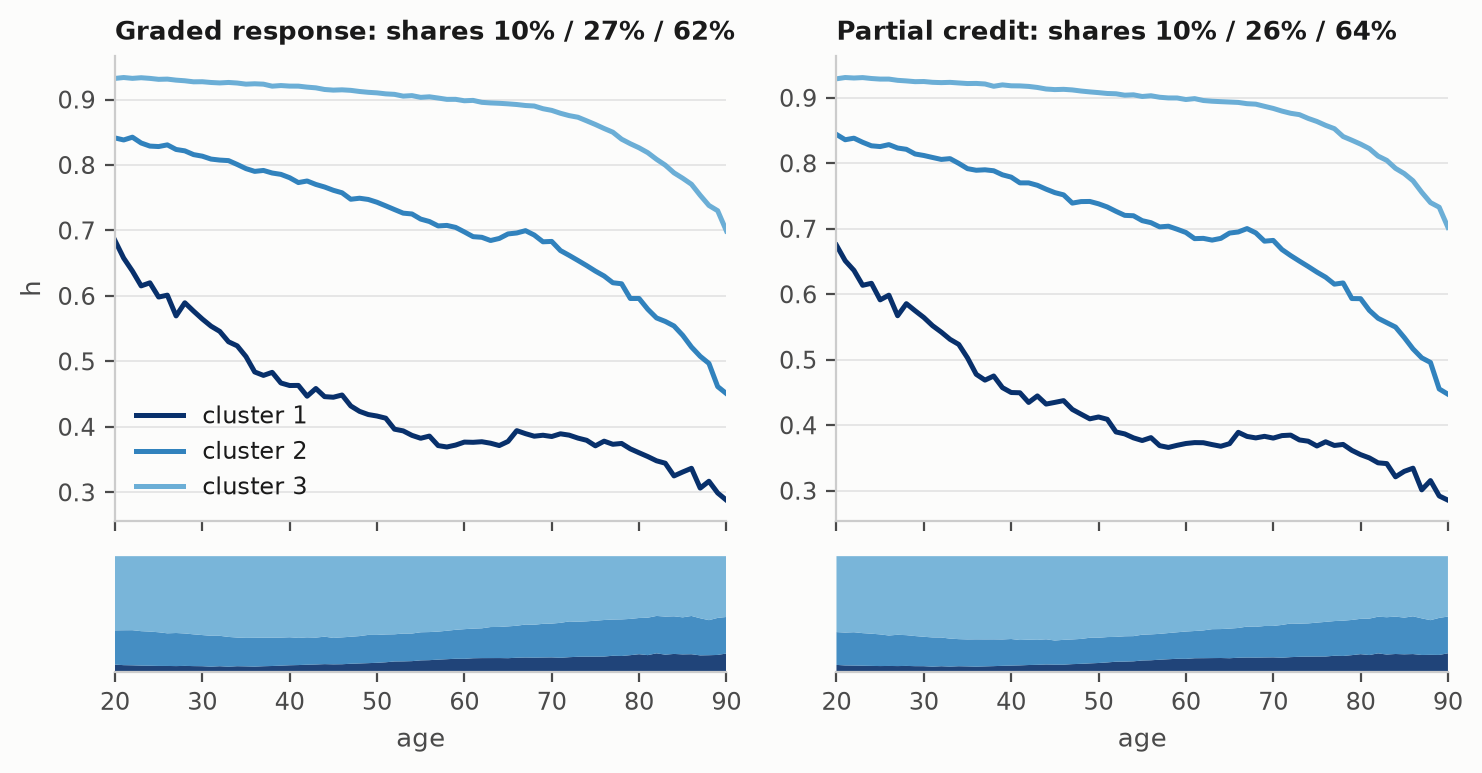
\includegraphics[width=\linewidth]{fig_lim_clusters_plim4}
\caption{Partial K-means, $K=3$, for P-LIM4 on $h$, as
Figure~\ref{fig:lim_cl_pfunc}.}
\label{fig:lim_cl_plim4}
\end{figure}

\subsubsection{P-LIM3}
Each testlet has a name in the disablement literature: functional
limitations (Verbrugge and Jette 1994), basic self-care as in the Katz
activities of daily living (Katz et al.\ 1963), and the senses. The floor
matches P-LIM4 at 0.02\%, with a stronger cost $t$ of 11.4 and no local
dependence above $+0.061$. Case 3's oldest-band correlation is $-0.17$; Case
2's is $+0.05$.

\begin{figure}[H]
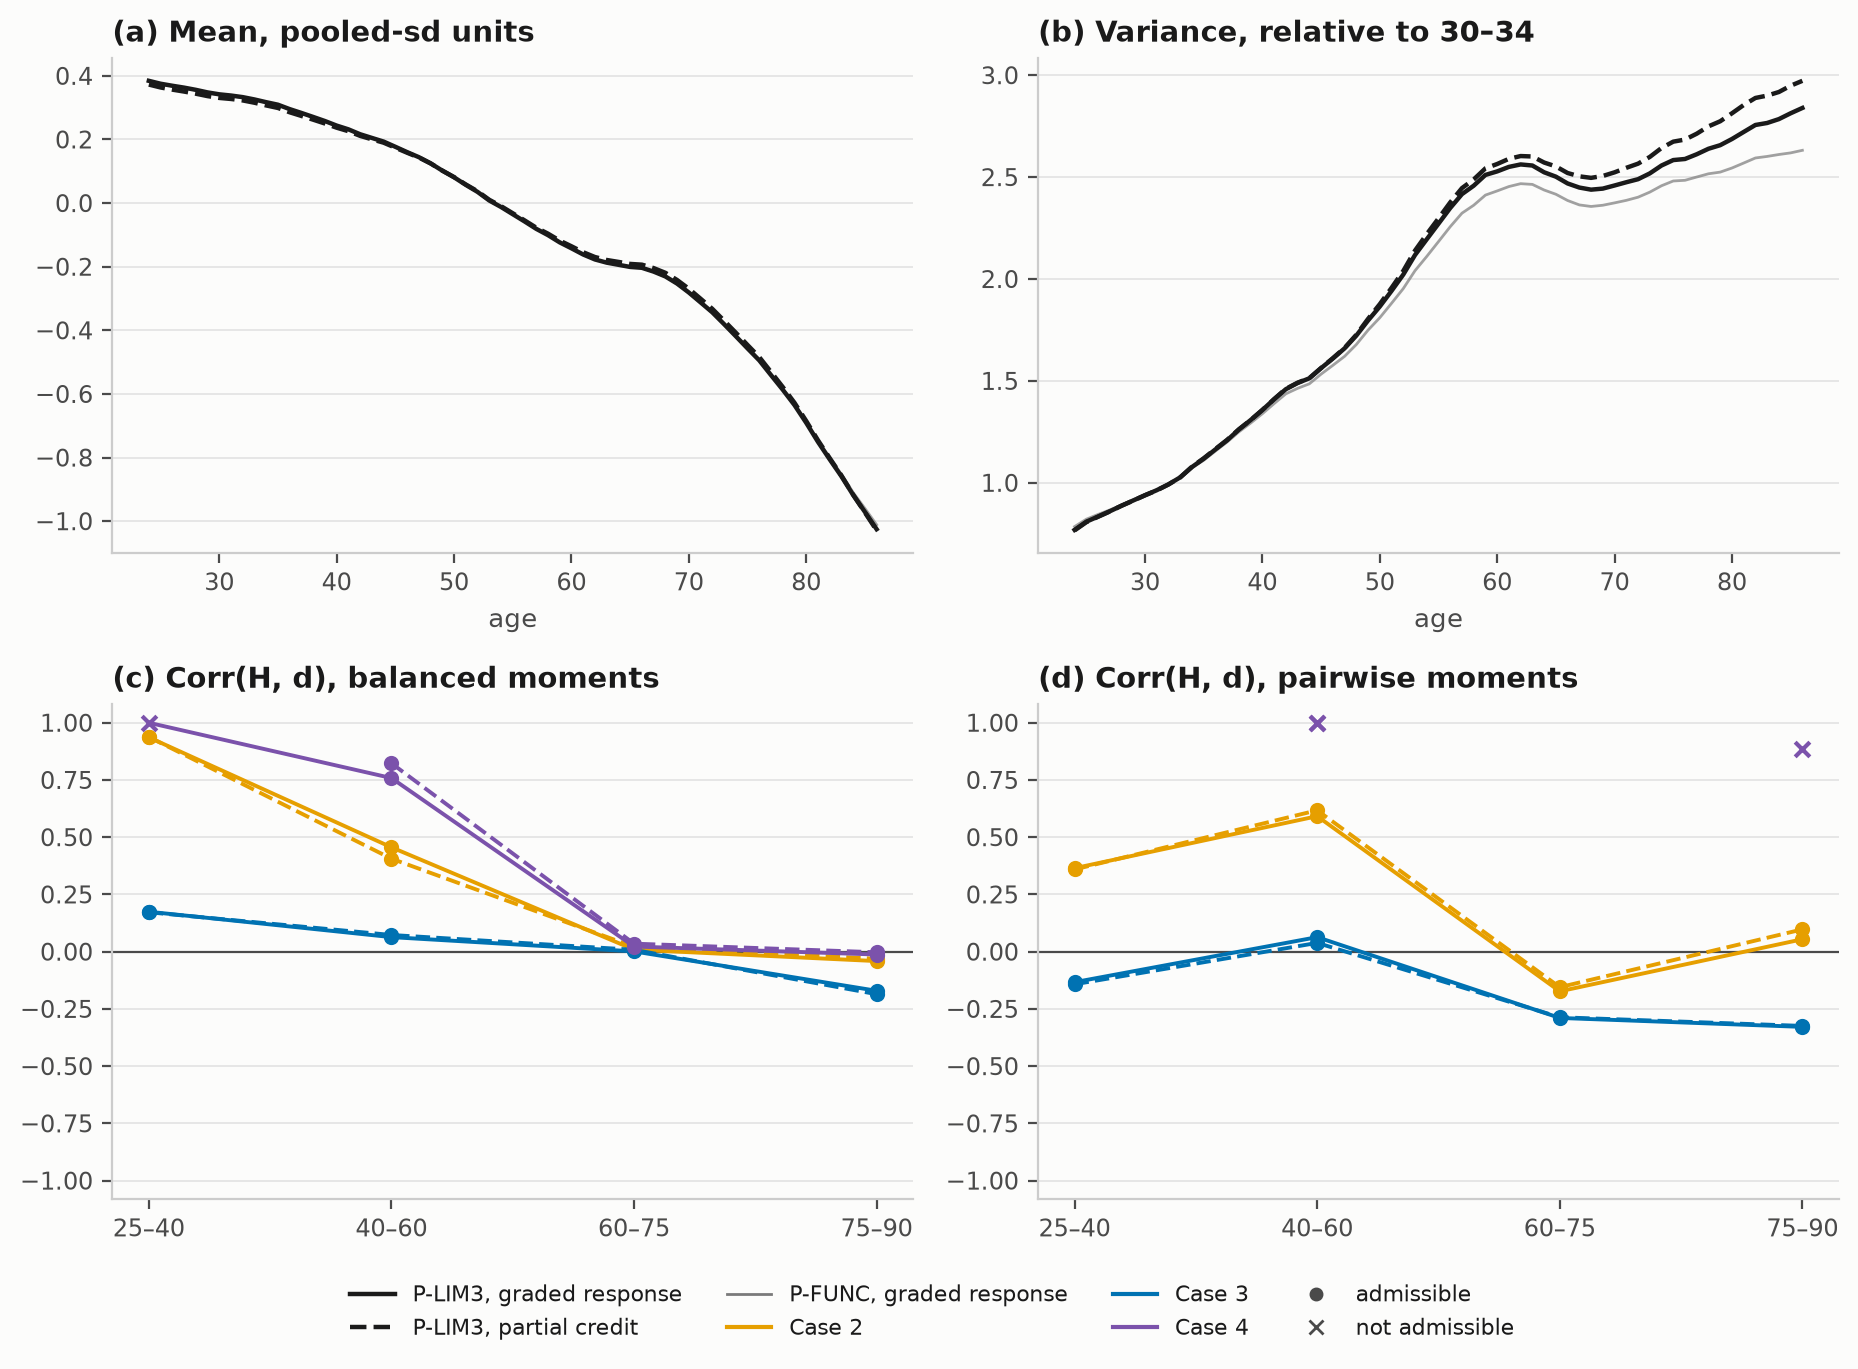
\includegraphics[width=\linewidth]{fig_lim_exhibit1_plim3}
\caption{Exhibit 1 for P-LIM3 on $h$, as Figure~\ref{fig:lim_ex1_plim1}.}
\label{fig:lim_ex1_plim3}
\end{figure}

\begin{figure}[H]
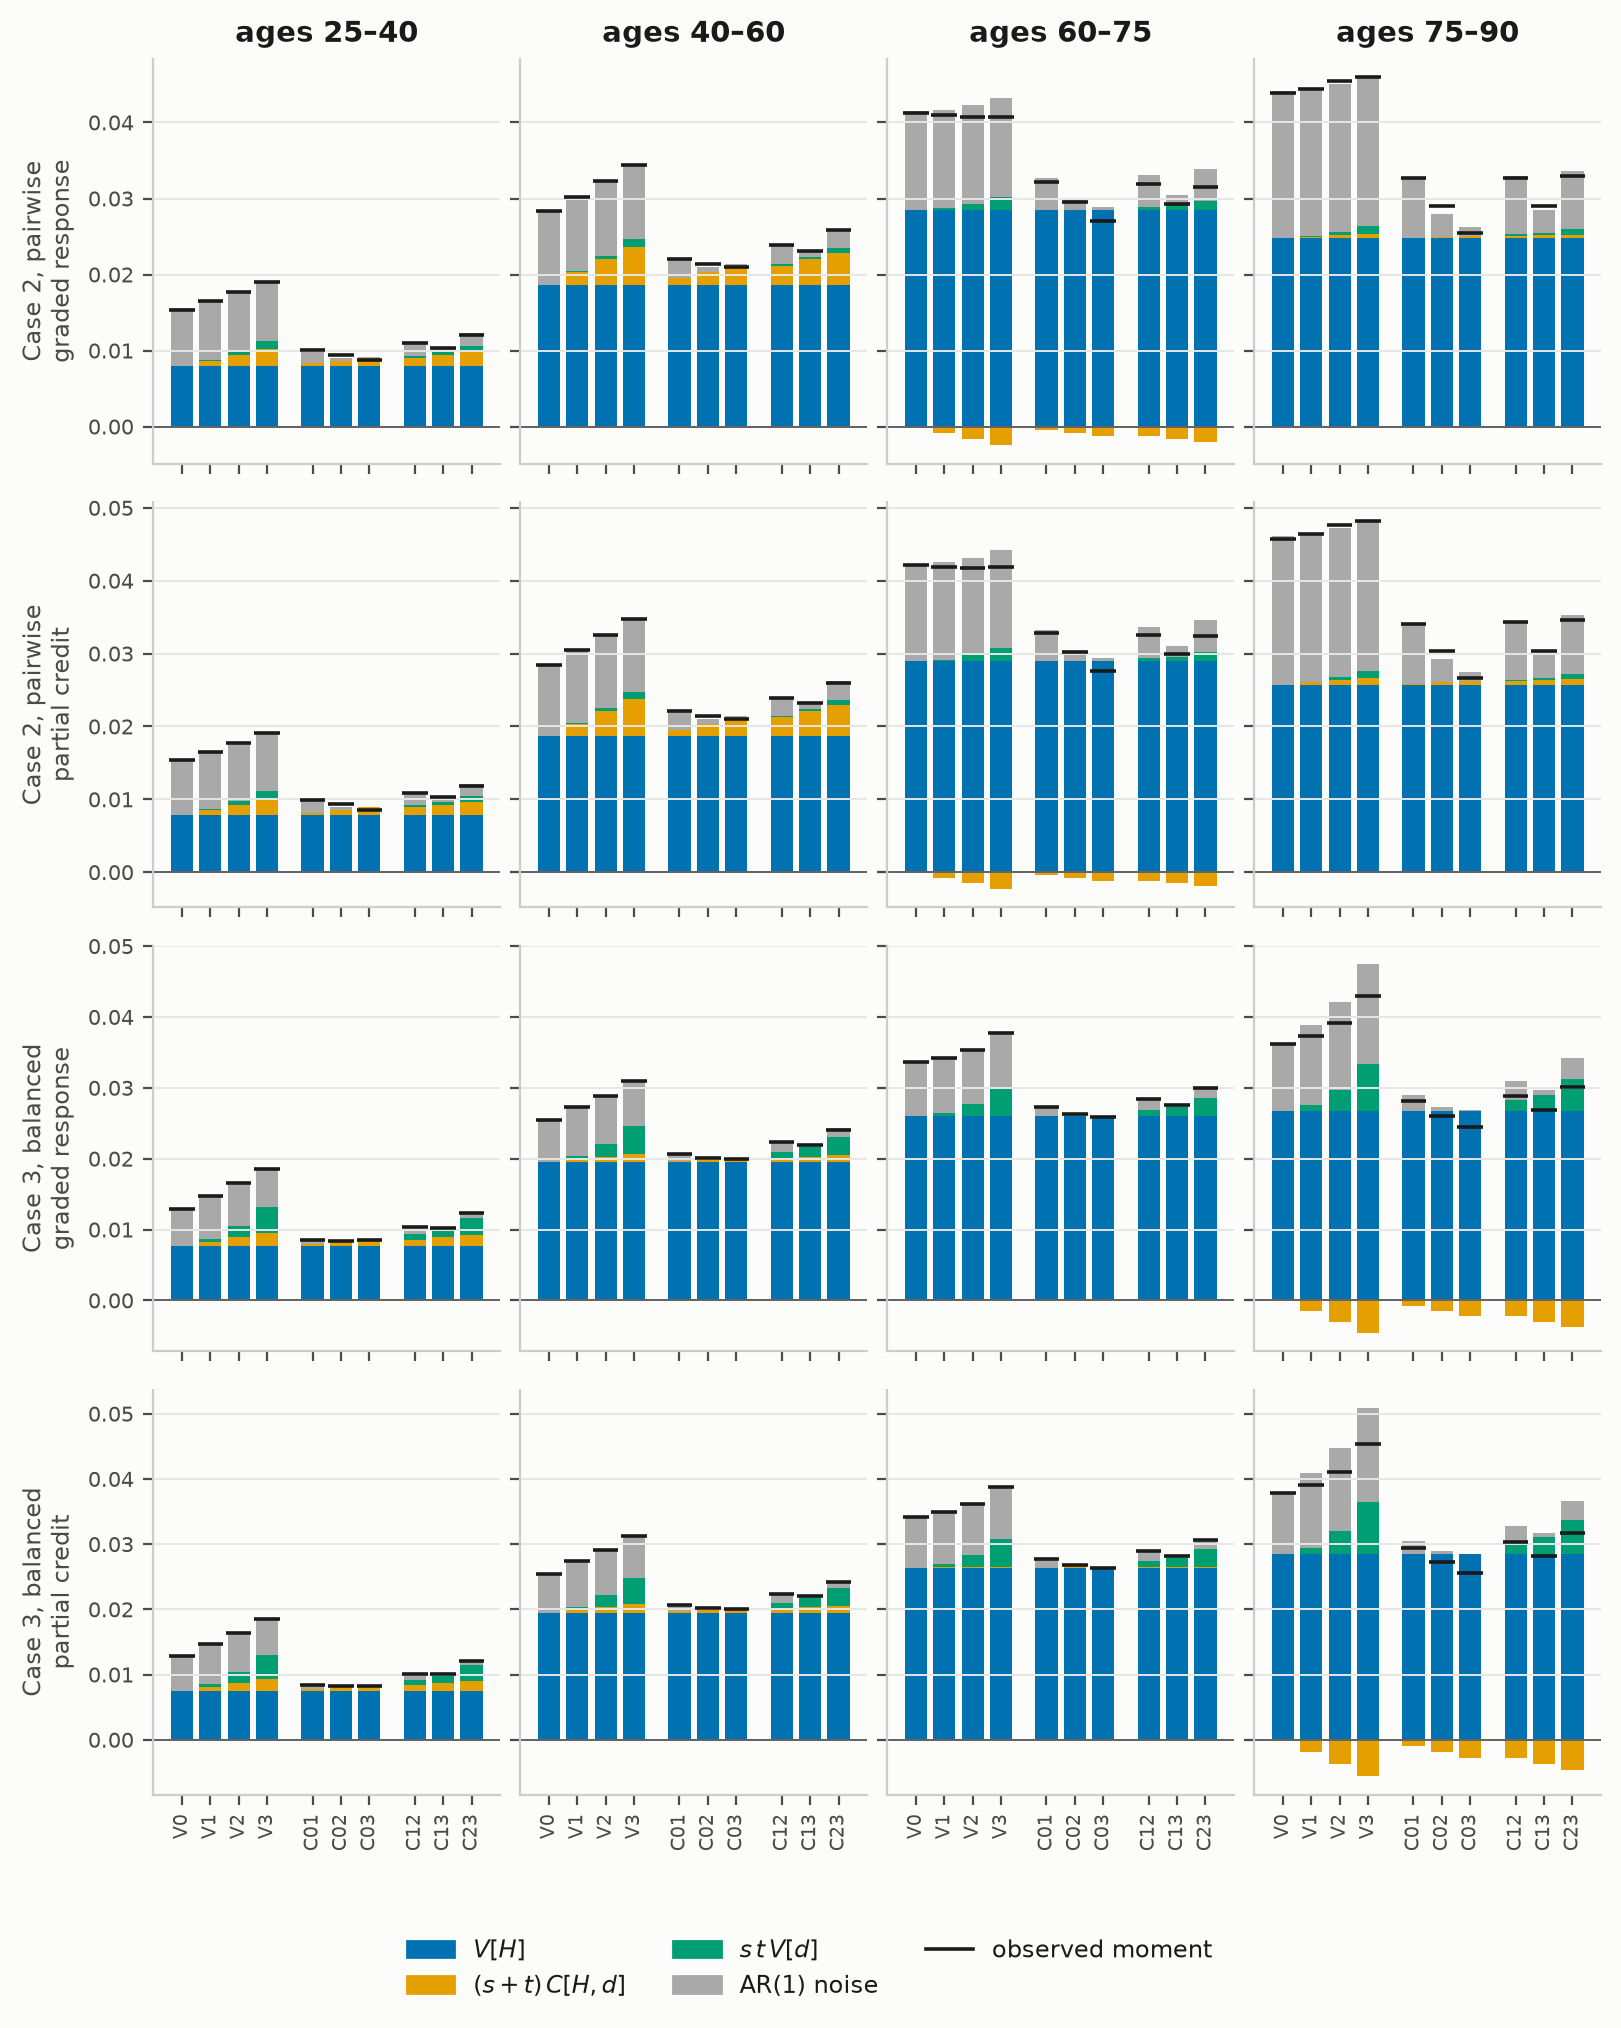
\includegraphics[width=\linewidth]{fig_lim_bars_plim3}
\caption{Identification barcharts for P-LIM3 on $h$, as
Figure~\ref{fig:lim_bars_pfunc}.}
\label{fig:lim_bars_plim3}
\end{figure}

\begin{figure}[H]
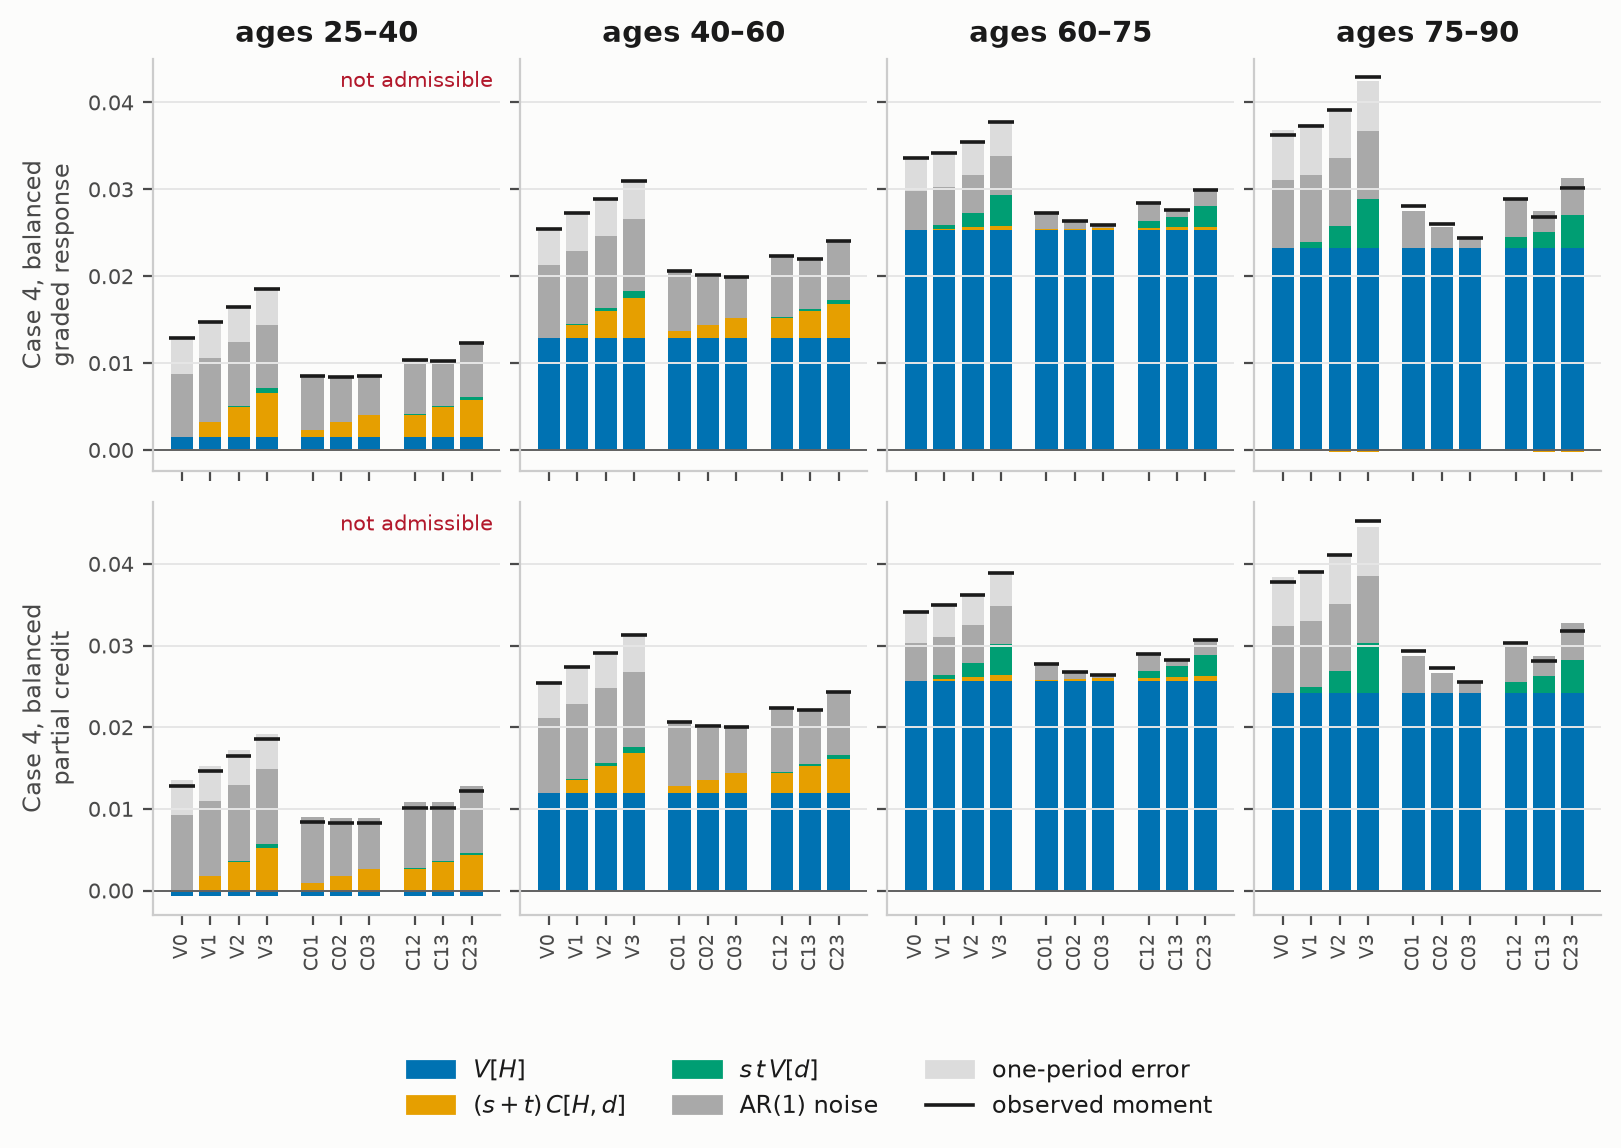
\includegraphics[width=\linewidth]{fig_lim_bars_case4_plim3}
\caption{Case 4 barcharts for P-LIM3 on $h$: balanced moments, noise split into
the AR(1) part and the one-period error.}
\label{fig:lim_bars4_plim3}
\end{figure}

\begin{figure}[H]
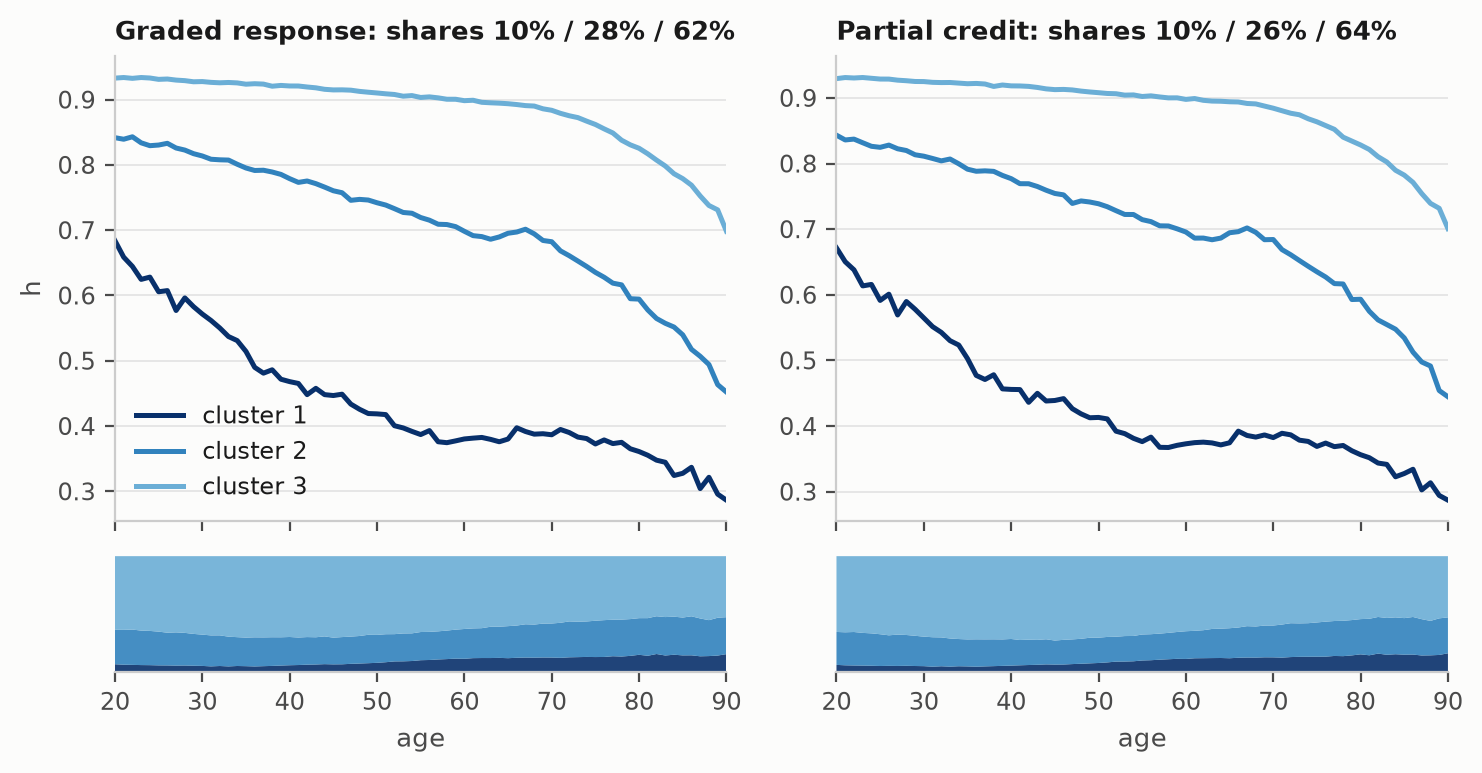
\includegraphics[width=\linewidth]{fig_lim_clusters_plim3}
\caption{Partial K-means, $K=3$, for P-LIM3 on $h$, as
Figure~\ref{fig:lim_cl_pfunc}.}
\label{fig:lim_cl_plim3}
\end{figure}

\subsubsection{P-LIM3+O}
The non-specific item takes the floor from 0.02\% to 0.01\% with 3\% of
observed weight. Its small residual dependence with general health, $+0.074$,
fits it picking up more than physical function. Every other criterion is
close to P-LIM3's.

\begin{figure}[H]
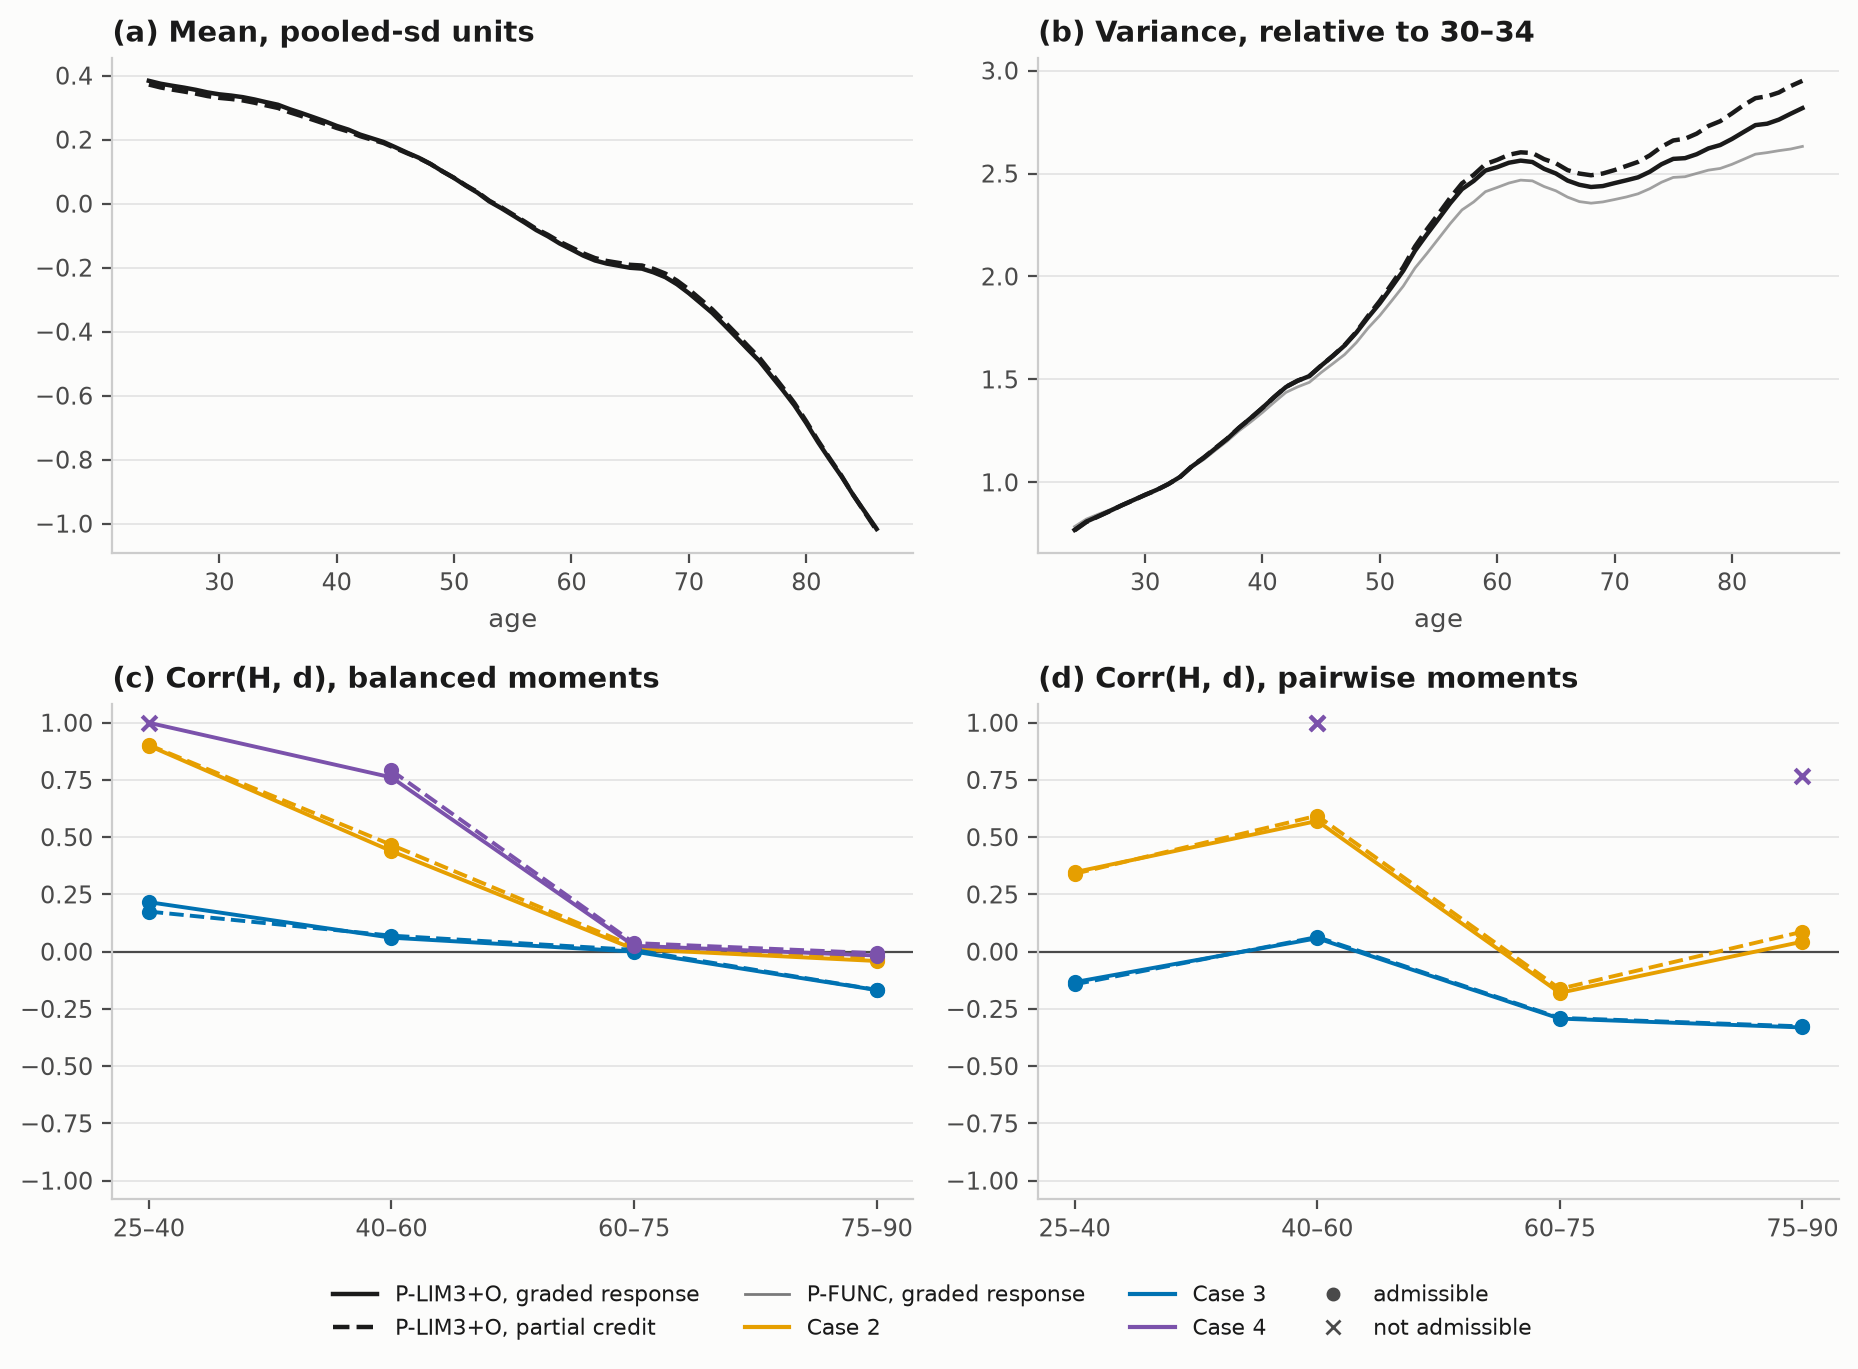
\includegraphics[width=\linewidth]{fig_lim_exhibit1_plim3o}
\caption{Exhibit 1 for P-LIM3+O on $h$, as Figure~\ref{fig:lim_ex1_plim1}.}
\label{fig:lim_ex1_plim3o}
\end{figure}

\begin{figure}[H]
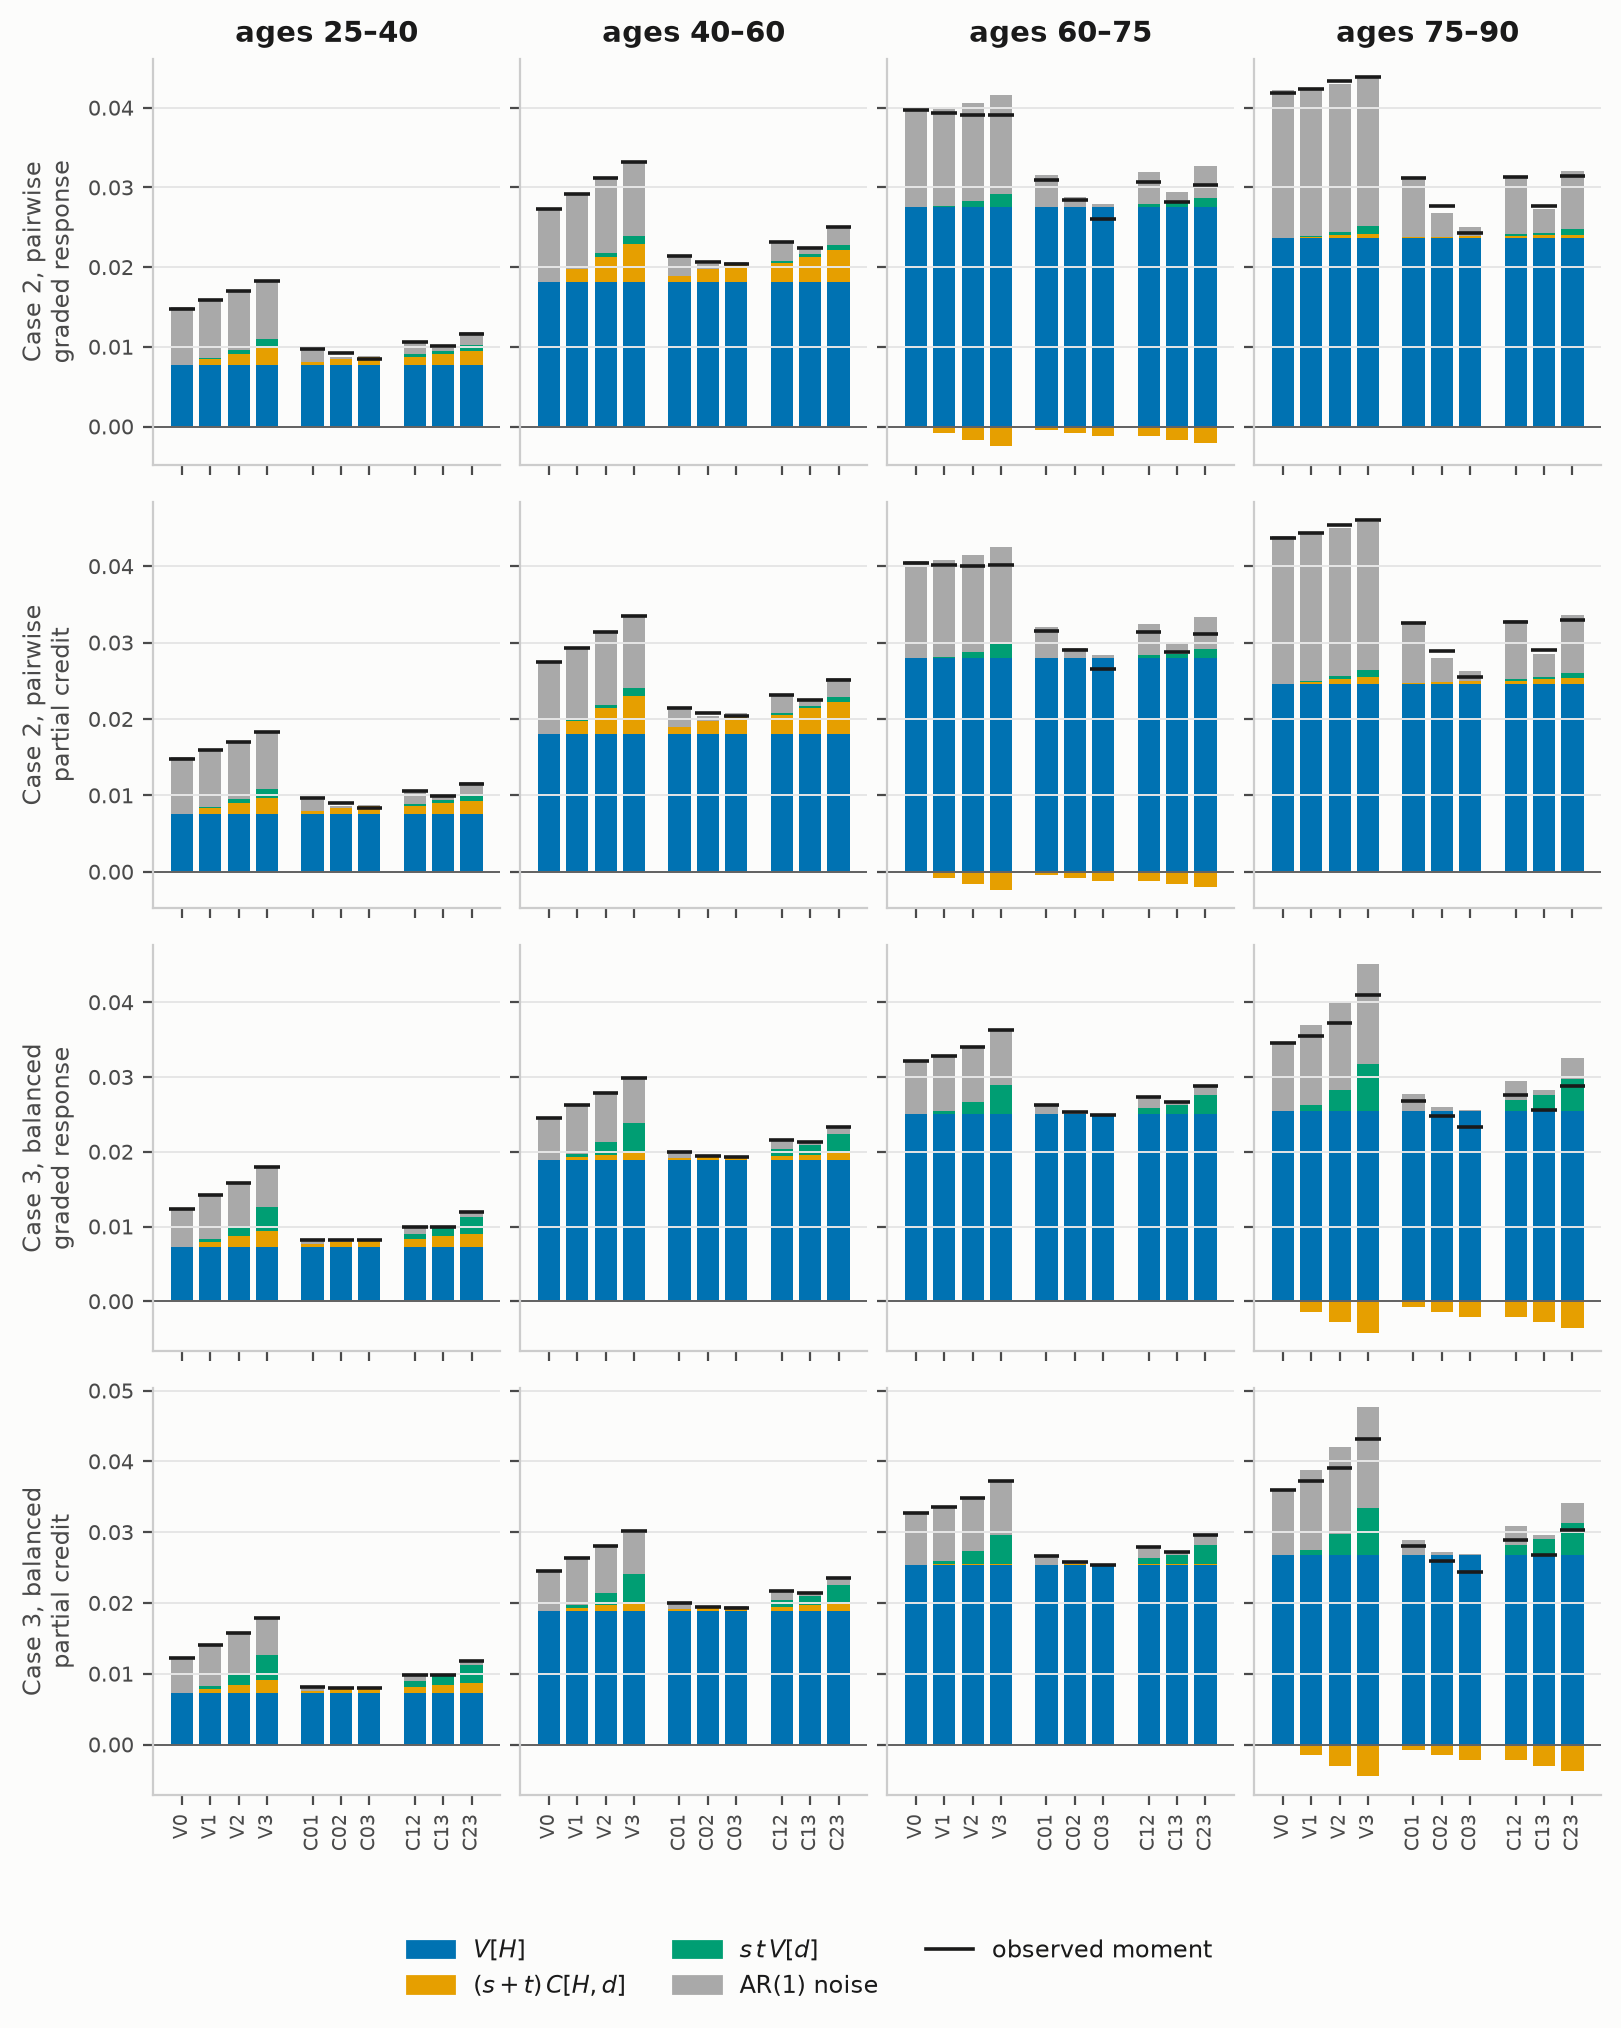
\includegraphics[width=\linewidth]{fig_lim_bars_plim3o}
\caption{Identification barcharts for P-LIM3+O on $h$, as
Figure~\ref{fig:lim_bars_pfunc}.}
\label{fig:lim_bars_plim3o}
\end{figure}

\begin{figure}[H]
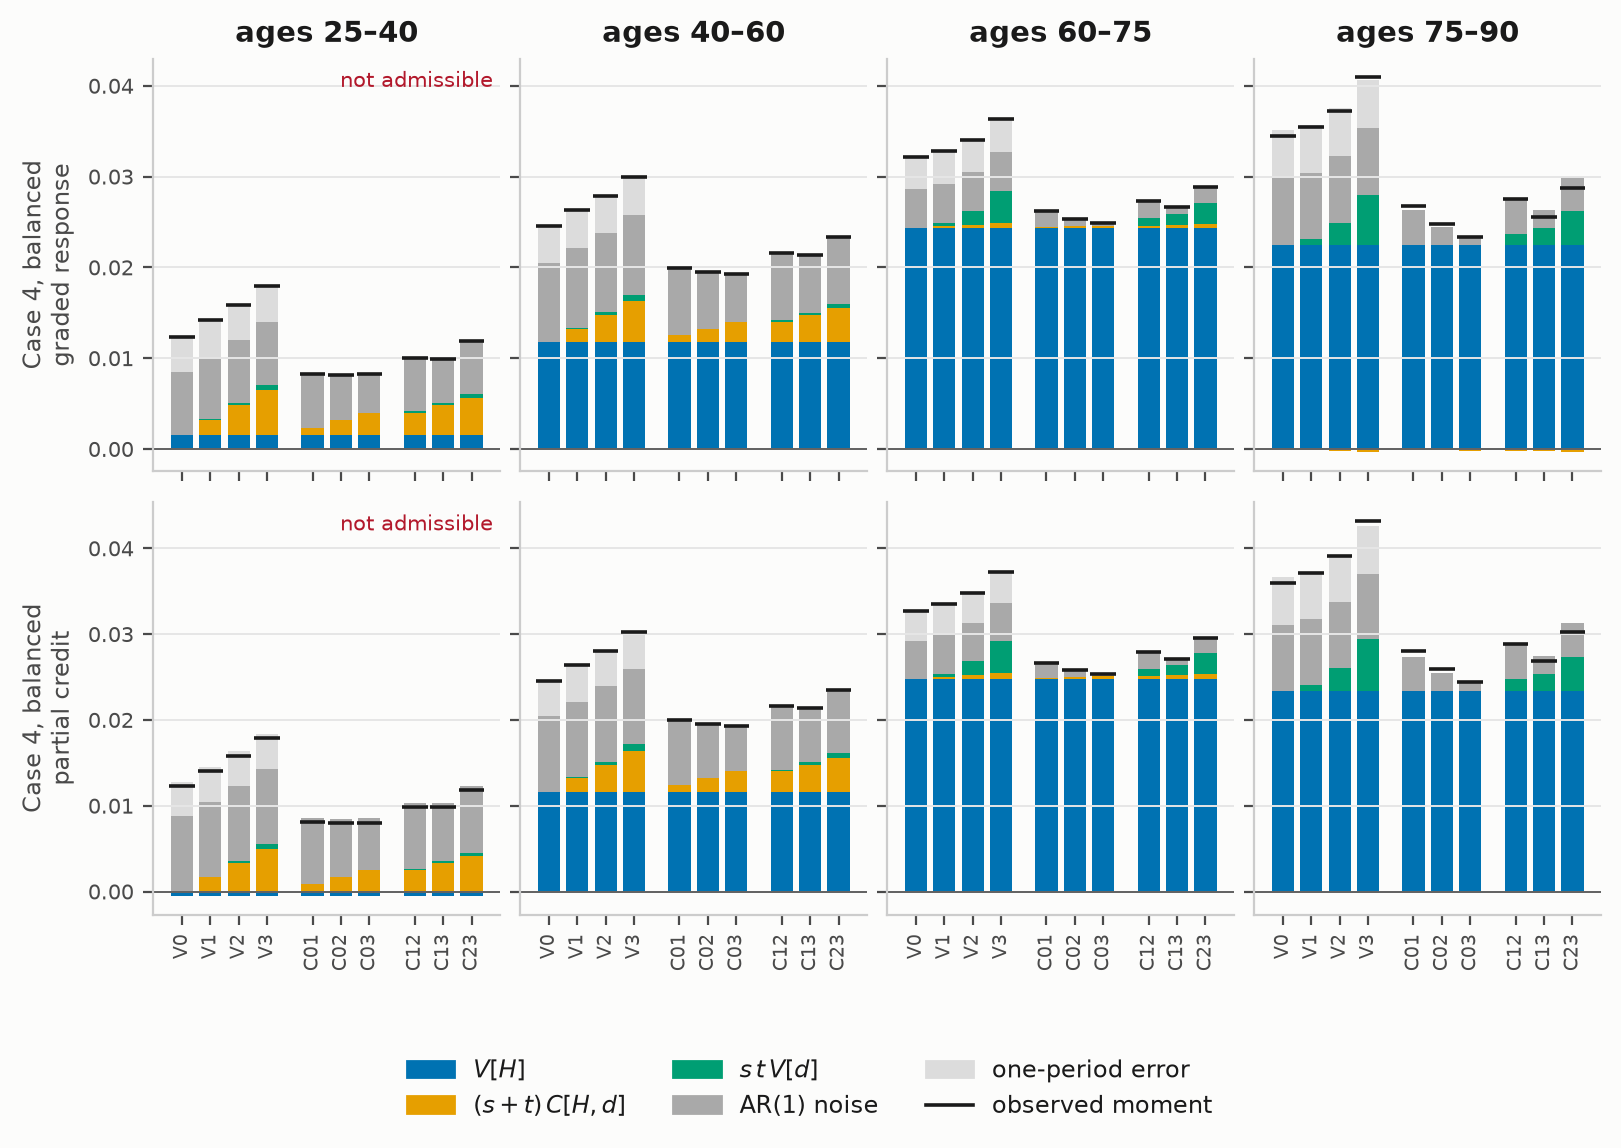
\includegraphics[width=\linewidth]{fig_lim_bars_case4_plim3o}
\caption{Case 4 barcharts for P-LIM3+O on $h$: balanced moments, noise split into
the AR(1) part and the one-period error.}
\label{fig:lim_bars4_plim3o}
\end{figure}

\begin{figure}[H]
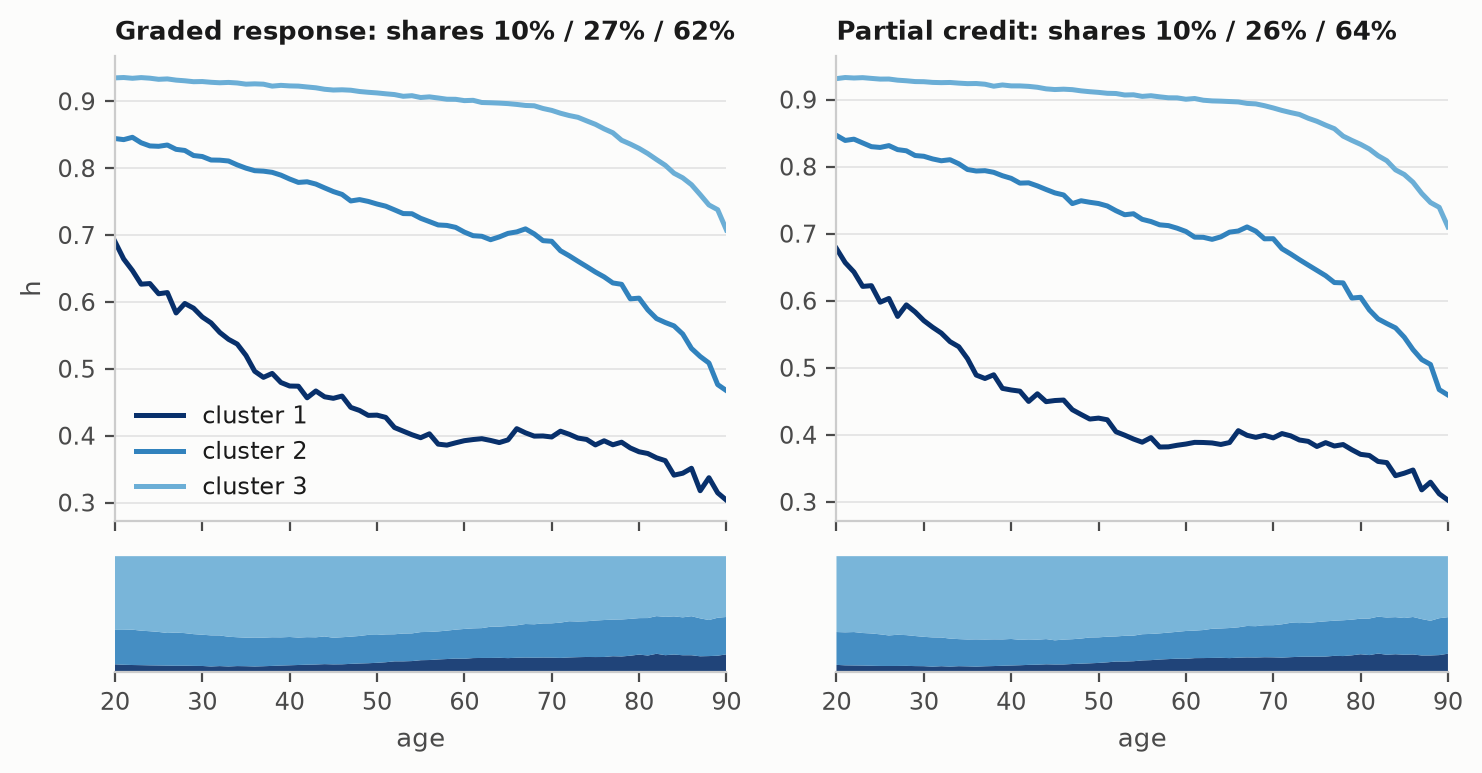
\includegraphics[width=\linewidth]{fig_lim_clusters_plim3o}
\caption{Partial K-means, $K=3$, for P-LIM3+O on $h$, as
Figure~\ref{fig:lim_cl_pfunc}.}
\label{fig:lim_cl_plim3o}
\end{figure}

\subsection{What this suggests}
\begin{itemize}\itemsep2pt
\item Uncapping the physical-function count does most of the work on the
floor. The further testlets finish the job with little weight, and none of
them creates local dependence.
\item P-LIM3 matches the finest split on the floor, with a clearer
description and stronger cost convexity. The non-specific item adds almost
nothing measurable and has no stated content.
\item The graded-response model fits better than partial credit in every bank.
Partial credit's exact weighted sum costs fit, weakens convexity on $h$, and
pushes Case 2's oldest band further positive. Its weights are nearly those
of the graded-response projection, so the transparency argument can be made
with that projection ($R^2$ 0.993) instead.
\item On $h$ every bank keeps the sign path on balanced moments under Cases 2,
3 and 4; on pairwise moments only P-FUNC's Case 2 under the graded-response
model keeps it. So the question for Exhibit 2 is less the scale than the
moments: pairwise moments give each cell its own set of people, and that is
enough to turn the sign at one end of the life course or the other. On
$\theta$ the pairwise Case 2 path survives, but Case 2 and Case 4 on balanced
moments stop being admissible.
\end{itemize}

\section{Adding chronic conditions to the limitation banks}
\label{sec:conbanks}

Each limitation bank of Section~\ref{sec:limbanks} except P-FUNC gets the
chronic conditions in two ways, both under the graded-response model. +CC
adds one testlet, the count of the sixteen ever-diagnosed physical conditions
(depression excluded), from 0 to 5 and 6 or more: seven or more hold 0.39\% of
person-waves and merge into six under the same rule as the limitation counts.
+CG adds P-FULL's six group items instead. P-FUNC with the six groups is P-FULL
itself, and refitting it reproduces P-FULL's scores exactly.

Conditions exist only from a person's first condition inventory, so all ten
banks use P-FULL's 387{,}599 person-waves from 69{,}958 people, and people
first interviewed at wave 2, mostly BHPS continuers, keep only 5\% of their
person-years. To separate the conditions from that change of sample, each
limitation bank without conditions is also scored on exactly those
person-waves (``same people'' below).

\begin{center}\footnotesize\setlength{\tabcolsep}{4pt}
\begin{tabular}{@{}>{\raggedright\arraybackslash}p{3.0cm}>{\raggedright\arraybackslash}p{5.2cm}l>{\raggedright\arraybackslash}p{4.6cm}@{}}
\toprule
Testlet & Conditions & Codes & \% with 0 / 1 / 2 / \dots \\
\midrule
Chronic count & all sixteen below & 0--5, 6+ & 48.28 / 28.88 / 12.90 / 5.59 / 2.44 / 1.05 / 0.86 \\
Heart disease, stroke & heart failure, coronary heart disease, angina, heart attack, stroke & 0, 1, 2+ & 92.38 / 5.17 / 2.45 \\
Diabetes, blood pressure & diabetes, high blood pressure & 0, 1, 2 & 73.91 / 22.09 / 4.00 \\
Asthma, bronchitis, emphysema & asthma, emphysema, chronic bronchitis & 0, 1, 2+ & 82.92 / 15.66 / 1.42 \\
Arthritis & arthritis & 0, 1 & 82.84 / 17.16 \\
Cancer & cancer & 0, 1 & 94.51 / 5.49 \\
Thyroid, liver, epilepsy & hyper- and hypothyroidism, liver condition, epilepsy & 0, 1+ & 91.30 / 8.70 \\
\bottomrule
\end{tabular}
\end{center}


\subsection{Fit and local dependence}

\begin{center}\footnotesize
\begin{tabular}{@{}lrrrl@{}}
\toprule
Bank & Testlets & Patterns & $\log L$ & Largest $Q_3$ \\
\midrule
P-LIM1+CC & 6 & 16{,}203 & $-2{,}418{,}571$ & $+0.025$, general health with the condition count \\
P-LIM1+CG & 11 & 47{,}469 & $-2{,}836{,}723$ & $+0.145$, heart disease with diabetes and blood pressure \\
P-LIM+CC & 7 & 24{,}370 & $-2{,}506{,}444$ & $+0.073$, limitations with sensory and continence \\
P-LIM+CG & 12 & 56{,}951 & $-2{,}924{,}370$ & $+0.144$, heart disease with diabetes and blood pressure \\
P-LIM4+CC & 9 & 31{,}411 & $-2{,}559{,}843$ & $+0.070$, mobility and lifting with dexterity and care \\
P-LIM4+CG & 14 & 62{,}497 & $-2{,}977{,}545$ & $+0.145$, heart disease with diabetes and blood pressure \\
P-LIM3+CC & 8 & 28{,}360 & $-2{,}535{,}876$ & $+0.052$, functional limitations with hearing and sight \\
P-LIM3+CG & 13 & 59{,}922 & $-2{,}953{,}756$ & $+0.145$, heart disease with diabetes and blood pressure \\
P-LIM3+O+CC & 9 & 35{,}403 & $-2{,}619{,}024$ & $+0.068$, general health with other problem \\
P-LIM3+O+CG & 14 & 67{,}345 & $-3{,}036{,}992$ & $+0.144$, heart disease with diabetes and blood pressure \\
\bottomrule
\end{tabular}
\end{center}


The count's discrimination is 1.17 to 1.19 in every bank, below any SF-12
testlet. The six groups keep their P-FULL values, from 0.41 for respiratory
conditions to 1.30 for arthritis. No bank shows local dependence: the count
banks' largest $Q_3$ is $+0.073$, between two limitation testlets, and the group
banks' is $+0.145$, heart disease with diabetes and blood pressure, as in
P-FULL.

\subsection{Criteria, with the people held fixed}
Columns are as in the limitation-bank criteria table, plus the share of
wave-2 entrants' person-years kept. Cost criteria use one common sample for
every measure in the workbook, which already requires a condition inventory,
so the ``same people'' rows need no separate cost figure. Their floor,
variance and identification entries are computed on the condition sample.

\begin{center}\footnotesize\setlength{\tabcolsep}{4pt}
\begin{tabular}{@{}lrrrrrccrrcc@{}}
\toprule
 & Wave-2 & Floor & Distinct & \multicolumn{4}{c}{$h$ scale} & \multicolumn{4}{c}{$\theta$ scale} \\
\cmidrule(lr){5-8}\cmidrule(l){9-12}
Bank & kept & 60--84 & 85--90 & Cost $t$ & Var. & C3 & C2 & Cost $t$ & Var. & C3 & C2 \\
\midrule
P-LIM1 & 100\% & 0.37\% & 98 & 13.2 & 1.08 & $\surd$ & $\times$ & 36.9 & 0.77 & $\surd$ & $\surd$ \\
\quad same people & 5\% & 0.38\% & 95 & & 1.06 & $\surd$ & $\surd$ & & & & \\
\quad +CC & 5\% & 0.08\% & 271 & 13.1 & 1.04 & $\surd$ & $\surd$ & 37.0 & 0.76 & $\surd$ & $\surd$ \\
\quad +CG & 5\% & 0.00\% & 479 & 12.5 & 1.05 & $\surd$ & $\surd$ & 38.3 & 0.74 & $\surd$ & $\surd$ \\
\addlinespace
P-LIM & 100\% & 0.10\% & 227 & 11.9 & 1.11 & $\surd$ & $\times$ & 36.9 & 0.78 & $\surd$ & $\surd$ \\
\quad same people & 5\% & 0.11\% & 204 & & 1.09 & $\surd$ & $\times$ & & & & \\
\quad +CC & 5\% & 0.03\% & 404 & 11.9 & 1.07 & $\surd$ & $\surd$ & 37.1 & 0.77 & $\surd$ & $\surd$ \\
\quad +CG & 5\% & 0.00\% & 514 & 11.3 & 1.08 & $\surd$ & $\times$ & 38.4 & 0.75 & $\surd$ & $\surd$ \\
\addlinespace
P-LIM4 & 100\% & 0.02\% & 344 & 10.6 & 1.13 & $\surd$ & $\times$ & 36.6 & 0.78 & $\surd$ & $\surd$ \\
\quad same people & 5\% & 0.02\% & 298 & & 1.10 & $\surd$ & $\times$ & & & & \\
\quad +CC & 5\% & 0.01\% & 451 & 10.5 & 1.08 & $\surd$ & $\surd$ & 36.7 & 0.77 & $\surd$ & $\surd$ \\
\quad +CG & 5\% & 0.00\% & 524 & 10.0 & 1.09 & $\surd$ & $\times$ & 38.0 & 0.75 & $\surd$ & $\surd$ \\
\addlinespace
P-LIM3 & 100\% & 0.02\% & 348 & 11.4 & 1.12 & $\surd$ & $\times$ & 36.8 & 0.78 & $\surd$ & $\surd$ \\
\quad same people & 5\% & 0.02\% & 298 & & 1.10 & $\surd$ & $\times$ & & & & \\
\quad +CC & 5\% & 0.01\% & 458 & 11.3 & 1.08 & $\surd$ & $\surd$ & 37.0 & 0.77 & $\surd$ & $\surd$ \\
\quad +CG & 5\% & 0.00\% & 525 & 10.8 & 1.09 & $\surd$ & $\times$ & 38.3 & 0.75 & $\surd$ & $\surd$ \\
\addlinespace
P-LIM3+O & 100\% & 0.01\% & 428 & 11.3 & 1.11 & $\surd$ & $\times$ & 37.4 & 0.77 & $\surd$ & $\surd$ \\
\quad same people & 5\% & 0.01\% & 358 & & 1.09 & $\surd$ & $\times$ & & & & \\
\quad +CC & 5\% & 0.00\% & 483 & 11.2 & 1.07 & $\surd$ & $\surd$ & 37.6 & 0.76 & $\surd$ & $\surd$ \\
\quad +CG & 5\% & 0.00\% & 531 & 10.7 & 1.08 & $\surd$ & $\times$ & 38.9 & 0.75 & $\surd$ & $\surd$ \\
\bottomrule
\end{tabular}
\end{center}


\begin{itemize}\itemsep2pt
\item \textbf{The count restores Case 2 on pairwise moments.} On the same
people, without conditions, only P-LIM1 has the pairwise sign path. With the
count every bank has it; with the six groups only P-LIM1 does. Dropping the
BHPS continuers already moves the oldest band's correlation from $+0.04$ to
$+0.05$ to between $+0.00$ and $+0.01$ in the four banks that start positive, and
the count takes it to $-0.02$ to $-0.05$ in all five.
\item \textbf{Variance flattens.} Growth from 60 to 85 is 1.04 to 1.08 with the
count, inside the flattening band for every bank, against 1.06 to 1.10 for the
same people without conditions and 1.05 to 1.09 with the groups.
\item \textbf{Convexity barely moves with the count.} Capped cost $t$ is 10.5
to 13.1 with the count, within 0.1 of each bank without conditions; the groups
take 0.6 to 0.7 off.
\item \textbf{The floor goes completely.} With the groups no score has more
than 0.003\% of 60 to 84 year olds at its worst value; with the count the
most is 0.08\%, for P-LIM1+CC.
\end{itemize}

\subsection{Identification under every estimator}
Symbols as in Section~\ref{sec:limident}. On $h$ the table shows each
limitation bank on the same people, then with the count and with the groups.

\begin{center}\footnotesize\setlength{\tabcolsep}{3.5pt}
\begin{tabular}{@{}lcrcrcrcrcrcr@{}}
\toprule
 & \multicolumn{6}{c}{Balanced moments} & \multicolumn{6}{c}{Pairwise moments} \\
\cmidrule(lr){2-7}\cmidrule(l){8-13}
 & \multicolumn{2}{c}{Case 2} & \multicolumn{2}{c}{Case 3} & \multicolumn{2}{c}{Case 4} & \multicolumn{2}{c}{Case 2} & \multicolumn{2}{c}{Case 3} & \multicolumn{2}{c}{Case 4} \\
Bank & path & 75--90 & path & 75--90 & path & 75--90 & path & 75--90 & path & 75--90 & path & 75--90 \\
\midrule
\multicolumn{13}{@{}l}{\emph{$h$ scale}} \\
P-LIM1, same people & $\surd$ & $-0.12$ & $\surd$ & $-0.19$ & $\surd^{\circ}$ & $-0.11$ & $\surd$ & $-0.02$ & $\times$ & $-0.32$ & $\times$ & $+0.16$ \\
\quad +CC & $\surd$ & $-0.10$ & $\surd$ & $-0.18$ & $\surd^{\circ}$ & $-0.10$ & $\surd$ & $-0.05$ & $\times$ & $-0.31$ & $\times$ & $+0.11$ \\
\quad +CG & $\surd$ & $-0.09$ & $\surd$ & $-0.15$ & $\surd^{\circ}$ & $-0.08$ & $\surd$ & $-0.02$ & $\times$ & $-0.30$ & $\times$ & $+0.15$ \\
P-LIM, same people & $\surd$ & $-0.11$ & $\surd$ & $-0.16$ & $\surd^{\circ}$ & $-0.11$ & $\times$ & $+0.00$ & $\times$ & $-0.30$ & $\times$ & $+0.17$ \\
\quad +CC & $\surd$ & $-0.09$ & $\surd$ & $-0.16$ & $\surd^{\circ}$ & $-0.10$ & $\surd$ & $-0.03$ & $\times$ & $-0.30$ & $\times$ & $+0.14$ \\
\quad +CG & $\surd$ & $-0.08$ & $\surd$ & $-0.14$ & $\surd^{\circ}$ & $-0.08$ & $\times$ & $+0.01$ & $\times$ & $-0.29$ & $\times$ & $+0.21$ \\
P-LIM4, same people & $\surd$ & $-0.10$ & $\surd$ & $-0.17$ & $\surd^{\circ}$ & $-0.10$ & $\times$ & $+0.01$ & $\times$ & $-0.30$ & $\times$ & $+0.22$ \\
\quad +CC & $\surd$ & $-0.09$ & $\surd$ & $-0.16$ & $\surd^{\circ}$ & $-0.09$ & $\surd$ & $-0.02$ & $\times$ & $-0.29$ & $\times$ & $+0.17$ \\
\quad +CG & $\surd$ & $-0.08$ & $\surd$ & $-0.15$ & $\surd^{\circ}$ & $-0.08$ & $\times$ & $+0.03$ & $\times$ & $-0.29$ & $\times$ & $+0.23$ \\
P-LIM3, same people & $\surd$ & $-0.11$ & $\surd$ & $-0.16$ & $\surd^{\circ}$ & $-0.11$ & $\times$ & $+0.01$ & $\times$ & $-0.30$ & $\times$ & $+0.20$ \\
\quad +CC & $\surd$ & $-0.10$ & $\surd$ & $-0.15$ & $\surd^{\circ}$ & $-0.10$ & $\surd$ & $-0.02$ & $\times$ & $-0.29$ & $\times$ & $+0.14$ \\
\quad +CG & $\surd$ & $-0.08$ & $\surd$ & $-0.14$ & $\surd^{\circ}$ & $-0.09$ & $\times$ & $+0.02$ & $\times$ & $-0.29$ & $\times$ & $+0.18$ \\
P-LIM3+O, same people & $\surd$ & $-0.11$ & $\surd$ & $-0.15$ & $\surd^{\circ}$ & $-0.12$ & $\times$ & $+0.00$ & $\times$ & $-0.30$ & $\times$ & $+0.15$ \\
\quad +CC & $\surd$ & $-0.10$ & $\surd$ & $-0.15$ & $\surd^{\circ}$ & $-0.11$ & $\surd$ & $-0.03$ & $\times$ & $-0.29$ & $\times$ & $+0.12$ \\
\quad +CG & $\surd$ & $-0.09$ & $\surd$ & $-0.14$ & $\surd^{\circ}$ & $-0.09$ & $\times$ & $+0.01$ & $\times$ & $-0.29$ & $\times$ & $+0.16$ \\
\midrule
\multicolumn{13}{@{}l}{\emph{$\theta$ scale}} \\
P-LIM1+CC & $\surd$ & $-0.35$ & $\surd$ & $-0.34$ & $\surd^{\circ}$ & $-0.35$ & $\surd$ & $-0.32$ & $\times$ & $-0.35$ & $\surd^{\circ}$ & $-0.37$ \\
P-LIM1+CG & $\surd^{\circ}$ & $-0.37$ & $\surd$ & $-0.35$ & $\surd^{\circ}$ & $-0.38$ & $\surd$ & $-0.33$ & $\times$ & $-0.35$ & $\surd^{\circ}$ & $-0.40$ \\
P-LIM+CC & $\surd$ & $-0.35$ & $\surd$ & $-0.33$ & $\surd^{\circ}$ & $-0.35$ & $\surd$ & $-0.30$ & $\times$ & $-0.35$ & $\surd^{\circ}$ & $-0.35$ \\
P-LIM+CG & $\surd$ & $-0.37$ & $\surd$ & $-0.35$ & $\surd^{\circ}$ & $-0.37$ & $\surd$ & $-0.31$ & $\times$ & $-0.34$ & $\surd^{\circ}$ & $-0.38$ \\
P-LIM4+CC & $\surd$ & $-0.35$ & $\surd$ & $-0.34$ & $\surd^{\circ}$ & $-0.35$ & $\surd$ & $-0.30$ & $\times$ & $-0.34$ & $\surd^{\circ}$ & $-0.34$ \\
P-LIM4+CG & $\surd$ & $-0.37$ & $\surd$ & $-0.35$ & $\surd^{\circ}$ & $-0.37$ & $\surd$ & $-0.31$ & $\times$ & $-0.34$ & $\surd^{\circ}$ & $-0.37$ \\
P-LIM3+CC & $\surd$ & $-0.34$ & $\surd$ & $-0.33$ & $\surd^{\circ}$ & $-0.35$ & $\surd$ & $-0.30$ & $\times$ & $-0.34$ & $\surd^{\circ}$ & $-0.34$ \\
P-LIM3+CG & $\surd$ & $-0.37$ & $\surd$ & $-0.35$ & $\surd^{\circ}$ & $-0.37$ & $\surd$ & $-0.31$ & $\times$ & $-0.34$ & $\surd^{\circ}$ & $-0.38$ \\
P-LIM3+O+CC & $\surd$ & $-0.35$ & $\surd$ & $-0.33$ & $\surd^{\circ}$ & $-0.35$ & $\surd$ & $-0.30$ & $\times$ & $-0.34$ & $\surd^{\circ}$ & $-0.35$ \\
P-LIM3+O+CG & $\surd$ & $-0.37$ & $\surd$ & $-0.35$ & $\surd^{\circ}$ & $-0.37$ & $\surd$ & $-0.32$ & $\times$ & $-0.34$ & $\surd^{\circ}$ & $-0.38$ \\
\bottomrule
\end{tabular}
\end{center}


\begin{itemize}\itemsep2pt
\item On $h$ and balanced moments nothing changes: Cases 2 and 3 are signed
and admissible for every version, and Case 4 is signed but, as before, not
admissible at its best fit in every band.
\item On pairwise moments only Case 2 responds to the conditions, as above;
Case 3 still fails the youngest band and Case 4 the oldest.
\item On $\theta$ both codings keep the sign path under Case 3 on balanced and
Case 2 on pairwise moments, as the banks without conditions did.
\end{itemize}

\subsection{How much weight the conditions get}
Shares of weight on the condition testlets, defined as in
Section~\ref{sec:limbanks}. $R^2$ is that of the graded-response score
projected on the codes. The last column is the condition count's
discrimination, or the range across the six groups.

\begin{center}\footnotesize\setlength{\tabcolsep}{4pt}
\begin{tabular}{@{}lrrrrrrr@{}}
\toprule
 & \multicolumn{5}{c}{Share of weight on the condition testlets, \%} & & \\
\cmidrule(lr){2-6}
Bank & GRM, latent & Polychoric & GRM $h$ on codes & Pearson & First component & $R^2$ & Condition $a$ \\
\midrule
P-LIM1+CC & 5 & 5 & 7 & 7 & 14 & 0.992 & 1.17 \\
P-LIM1+CG & 17 & 16 & 15 & 15 & 34 & 0.993 & 0.41--1.29 \\
P-LIM+CC & 4 & 5 & 6 & 7 & 12 & 0.992 & 1.18 \\
P-LIM+CG & 16 & 15 & 15 & 15 & 32 & 0.993 & 0.41--1.30 \\
P-LIM4+CC & 3 & 3 & 6 & 6 & 10 & 0.993 & 1.19 \\
P-LIM4+CG & 12 & 11 & 14 & 14 & 27 & 0.993 & 0.41--1.31 \\
P-LIM3+CC & 4 & 4 & 6 & 6 & 11 & 0.993 & 1.18 \\
P-LIM3+CG & 14 & 14 & 14 & 14 & 29 & 0.993 & 0.41--1.30 \\
P-LIM3+O+CC & 4 & 4 & 6 & 6 & 10 & 0.993 & 1.19 \\
P-LIM3+O+CG & 14 & 14 & 14 & 14 & 28 & 0.993 & 0.41--1.30 \\
\bottomrule
\end{tabular}
\end{center}


\begin{itemize}\itemsep2pt
\item \textbf{The count is a light item.} It gets 3 to 5\% of latent weight and
6 to 7\% of observed weight. The six groups together get 11 to 17\% on either
scale, about three times the count's latent weight and twice its observed
weight, matching the 15\% the Pearson factor score gives conditions in P-FULL.
\item \textbf{The first principal component doubles both}, to 10 to 14\% for
the count and 27 to 34\% for the groups, because it does not discount weak
items.
\end{itemize}

\subsection{Figures by bank}
Each bank has four figures laid out as in Section~\ref{sec:limbanks}, with
the count solid and the groups dashed. The grey lines in Exhibit 1 are the
bank without conditions on the same people. The clusters use the 39{,}004
people with at least three observed ages in the condition sample. In every
bank the count and the groups put 98\% of them in the same cluster, with an
adjusted Rand index of 0.95, against 0.90 with the bank's clusters without
conditions.

\subsubsection{P-LIM1 with conditions}

\begin{figure}[H]
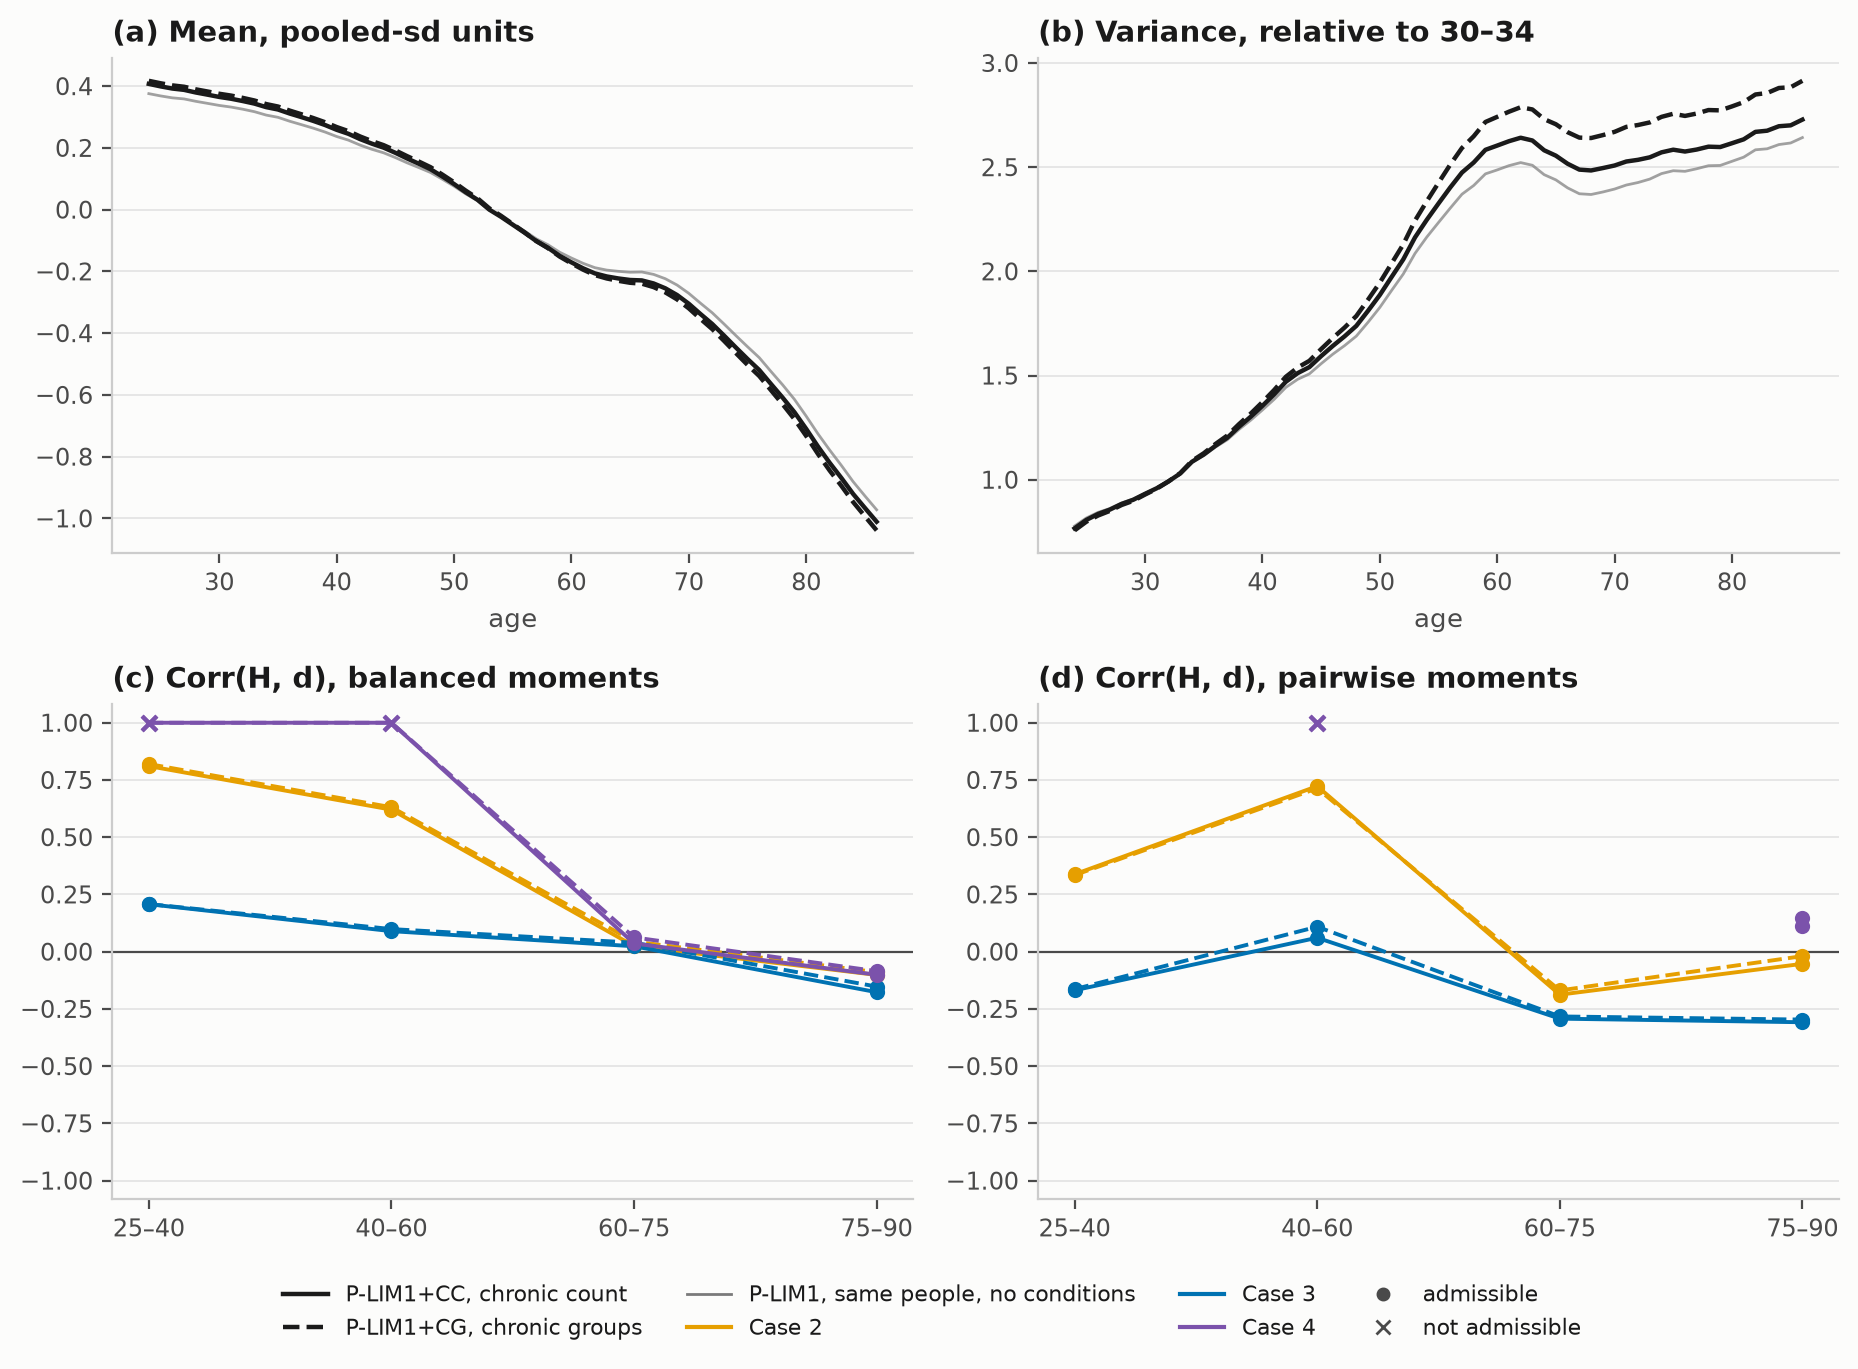
\includegraphics[width=\linewidth]{fig_con_exhibit1_plim1}
\caption{Exhibit 1 for P-LIM1+CC (solid) and P-LIM1+CG (dashed) on $h$, as
Figure~\ref{fig:lim_ex1_pfunc}; grey lines are P-LIM1 without conditions on the
same people.}
\label{fig:con_ex1_plim1}
\end{figure}

\begin{figure}[H]
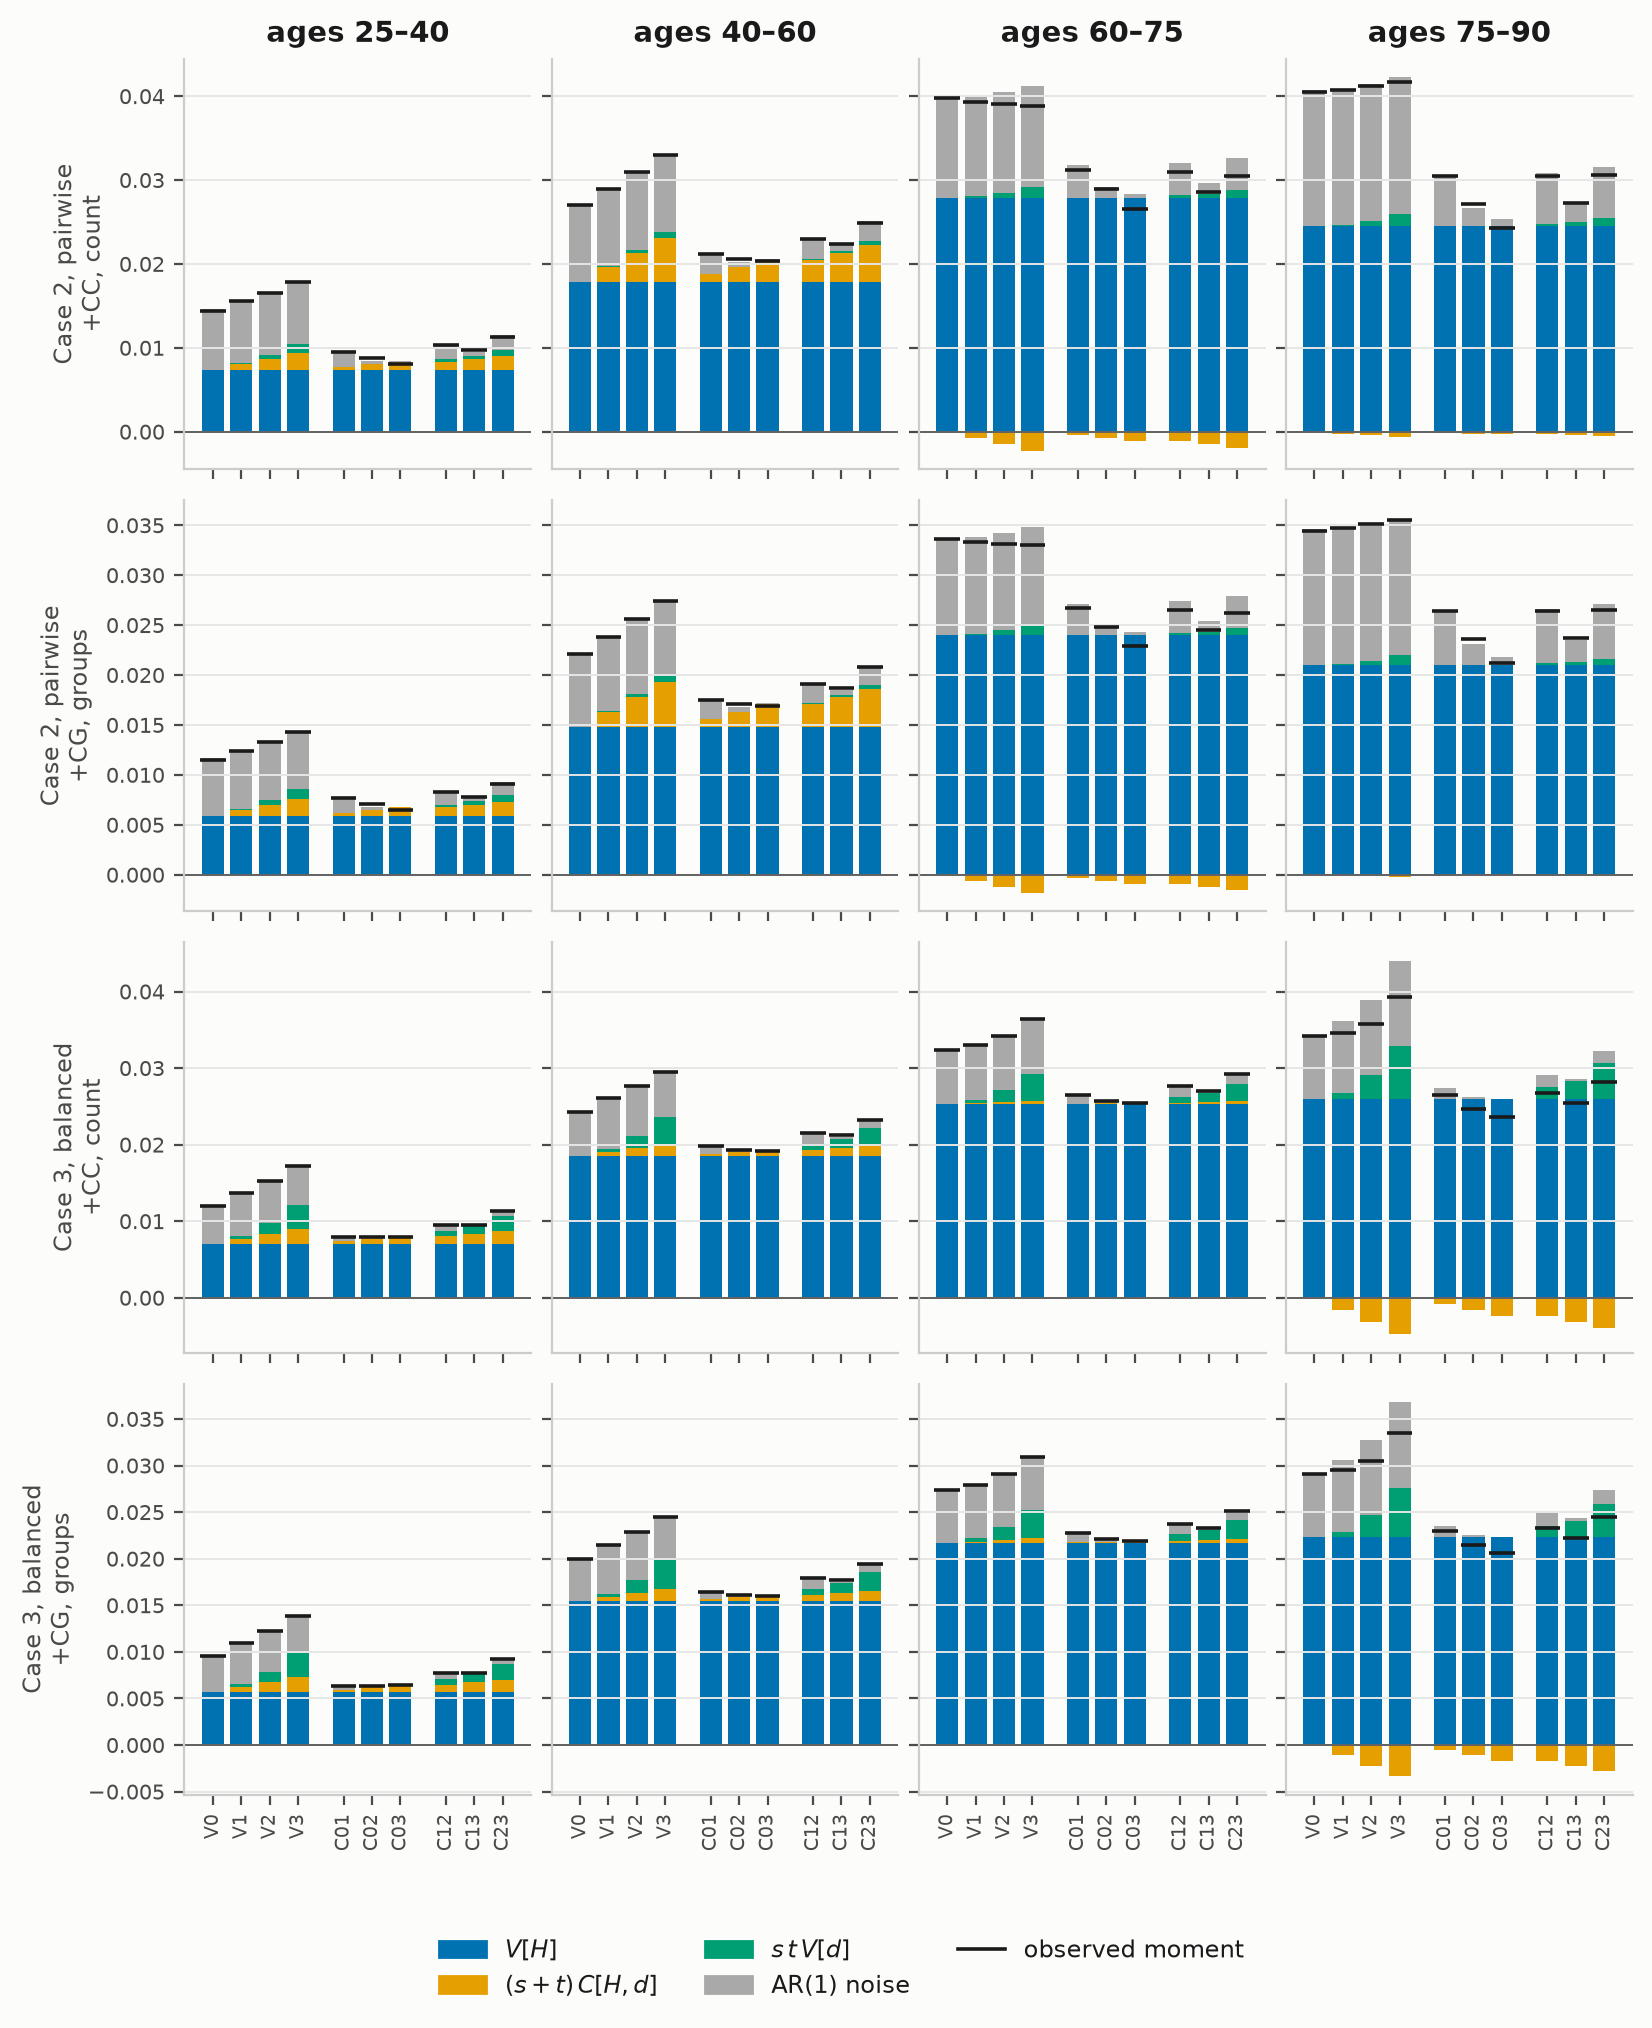
\includegraphics[width=\linewidth]{fig_con_bars_plim1}
\caption{Identification barcharts for P-LIM1+CC and P-LIM1+CG on $h$, as
Figure~\ref{fig:lim_bars_pfunc}.}
\label{fig:con_bars_plim1}
\end{figure}

\begin{figure}[H]
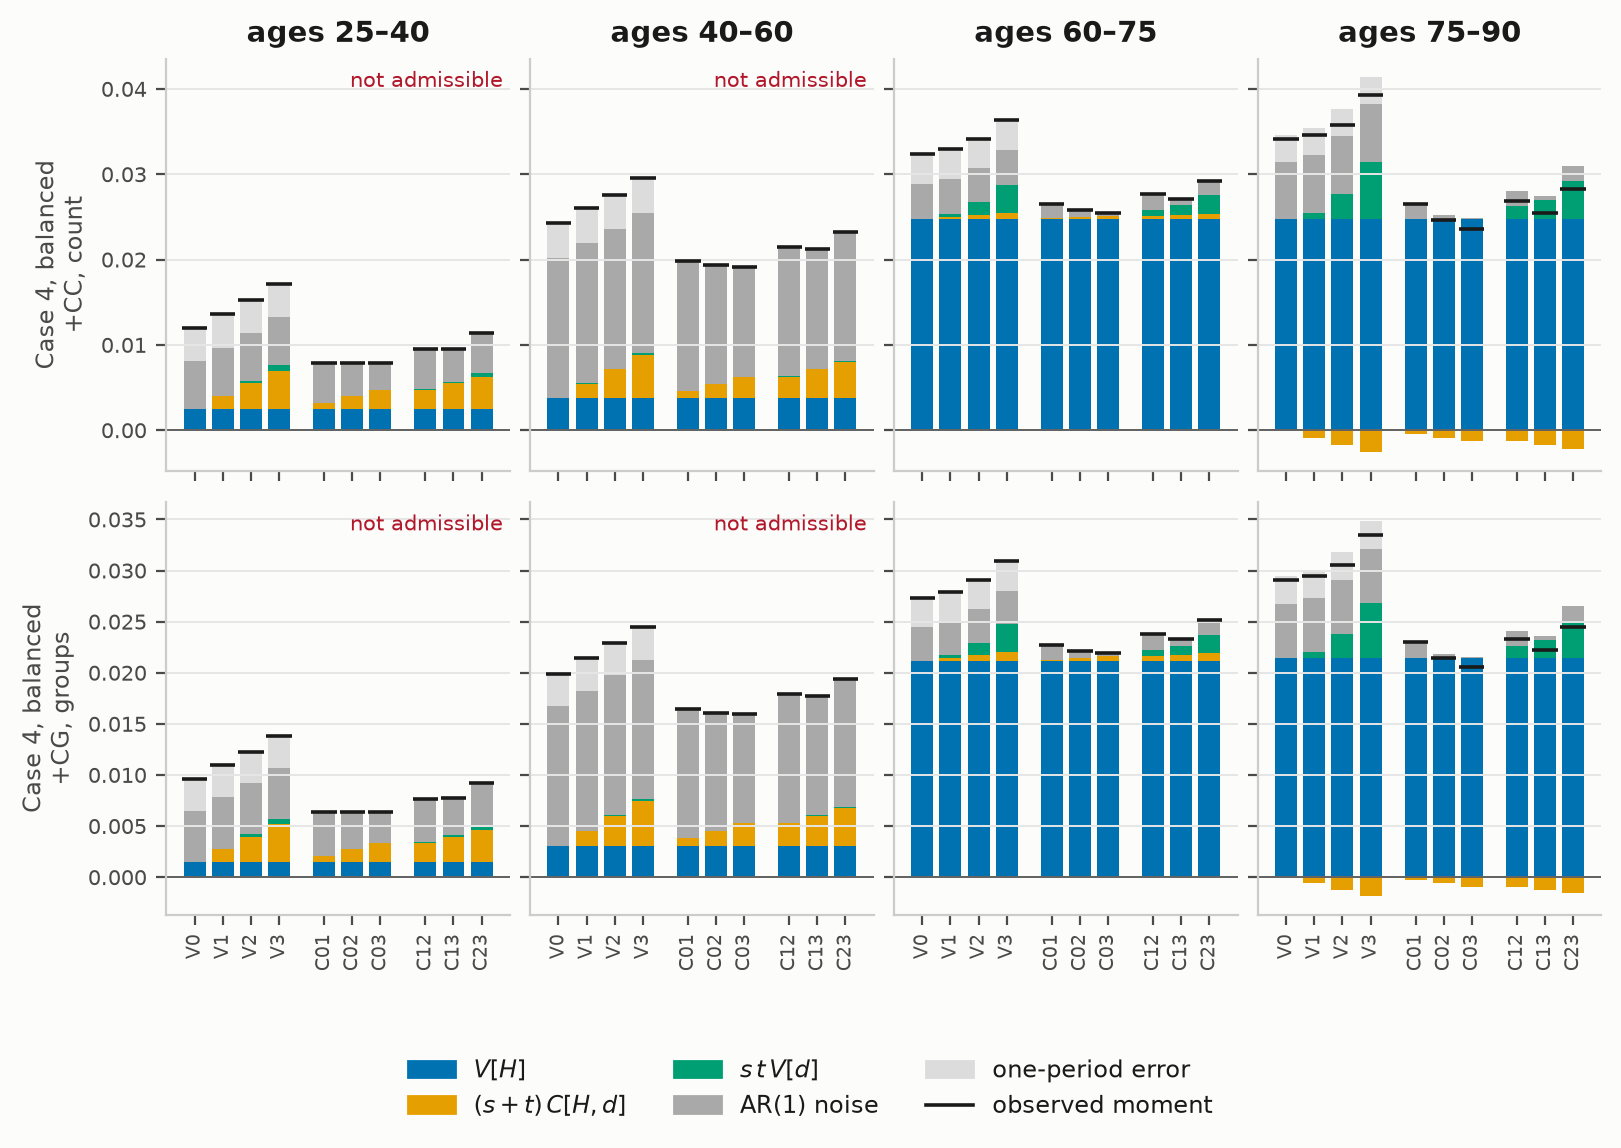
\includegraphics[width=\linewidth]{fig_con_bars_case4_plim1}
\caption{Case 4 barcharts for P-LIM1+CC and P-LIM1+CG on $h$, as
Figure~\ref{fig:lim_bars4_pfunc}.}
\label{fig:con_bars4_plim1}
\end{figure}

\begin{figure}[H]
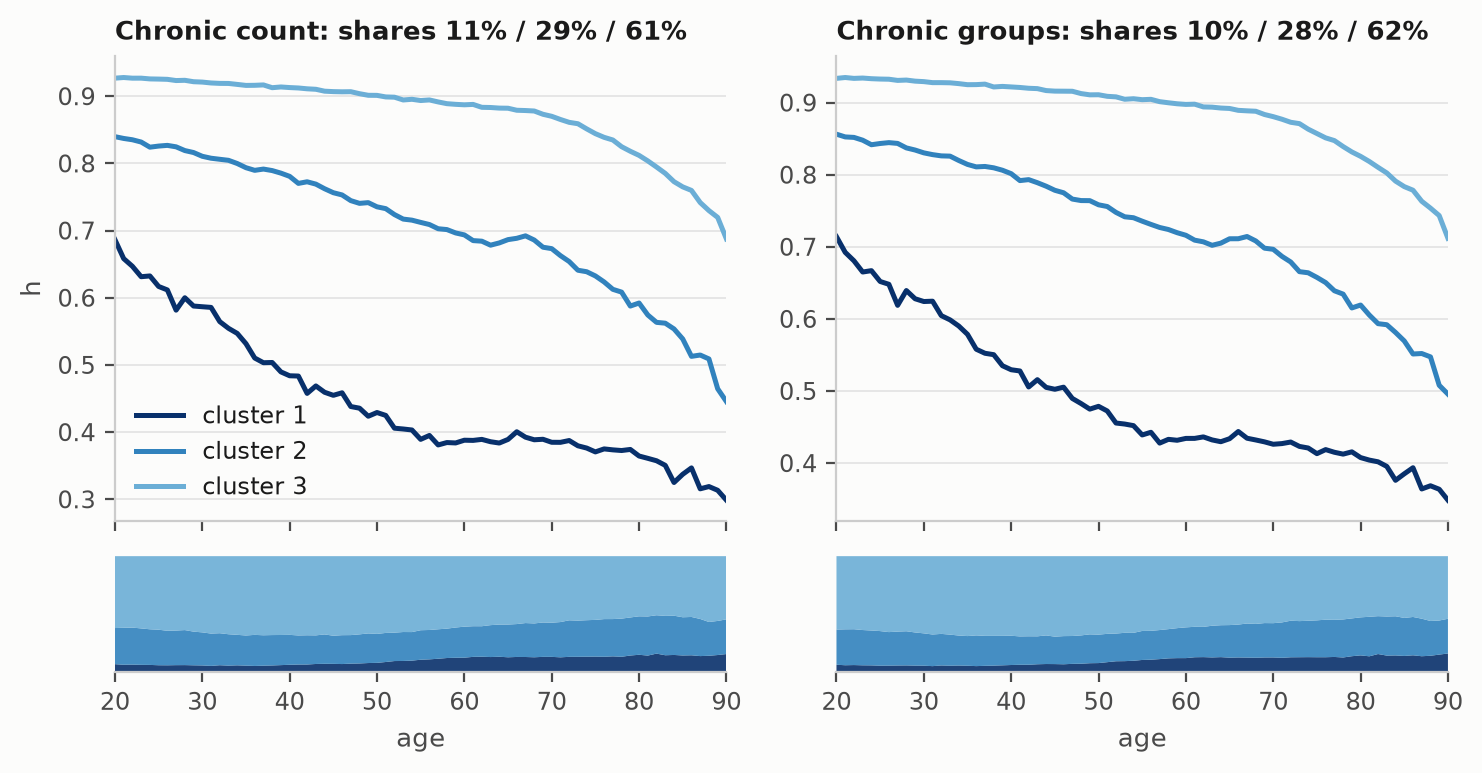
\includegraphics[width=\linewidth]{fig_con_clusters_plim1}
\caption{Partial K-means, $K=3$, for P-LIM1+CC (left) and P-LIM1+CG (right) on $h$,
as Figure~\ref{fig:lim_cl_pfunc}.}
\label{fig:con_cl_plim1}
\end{figure}

\subsubsection{P-LIM with conditions}

\begin{figure}[H]
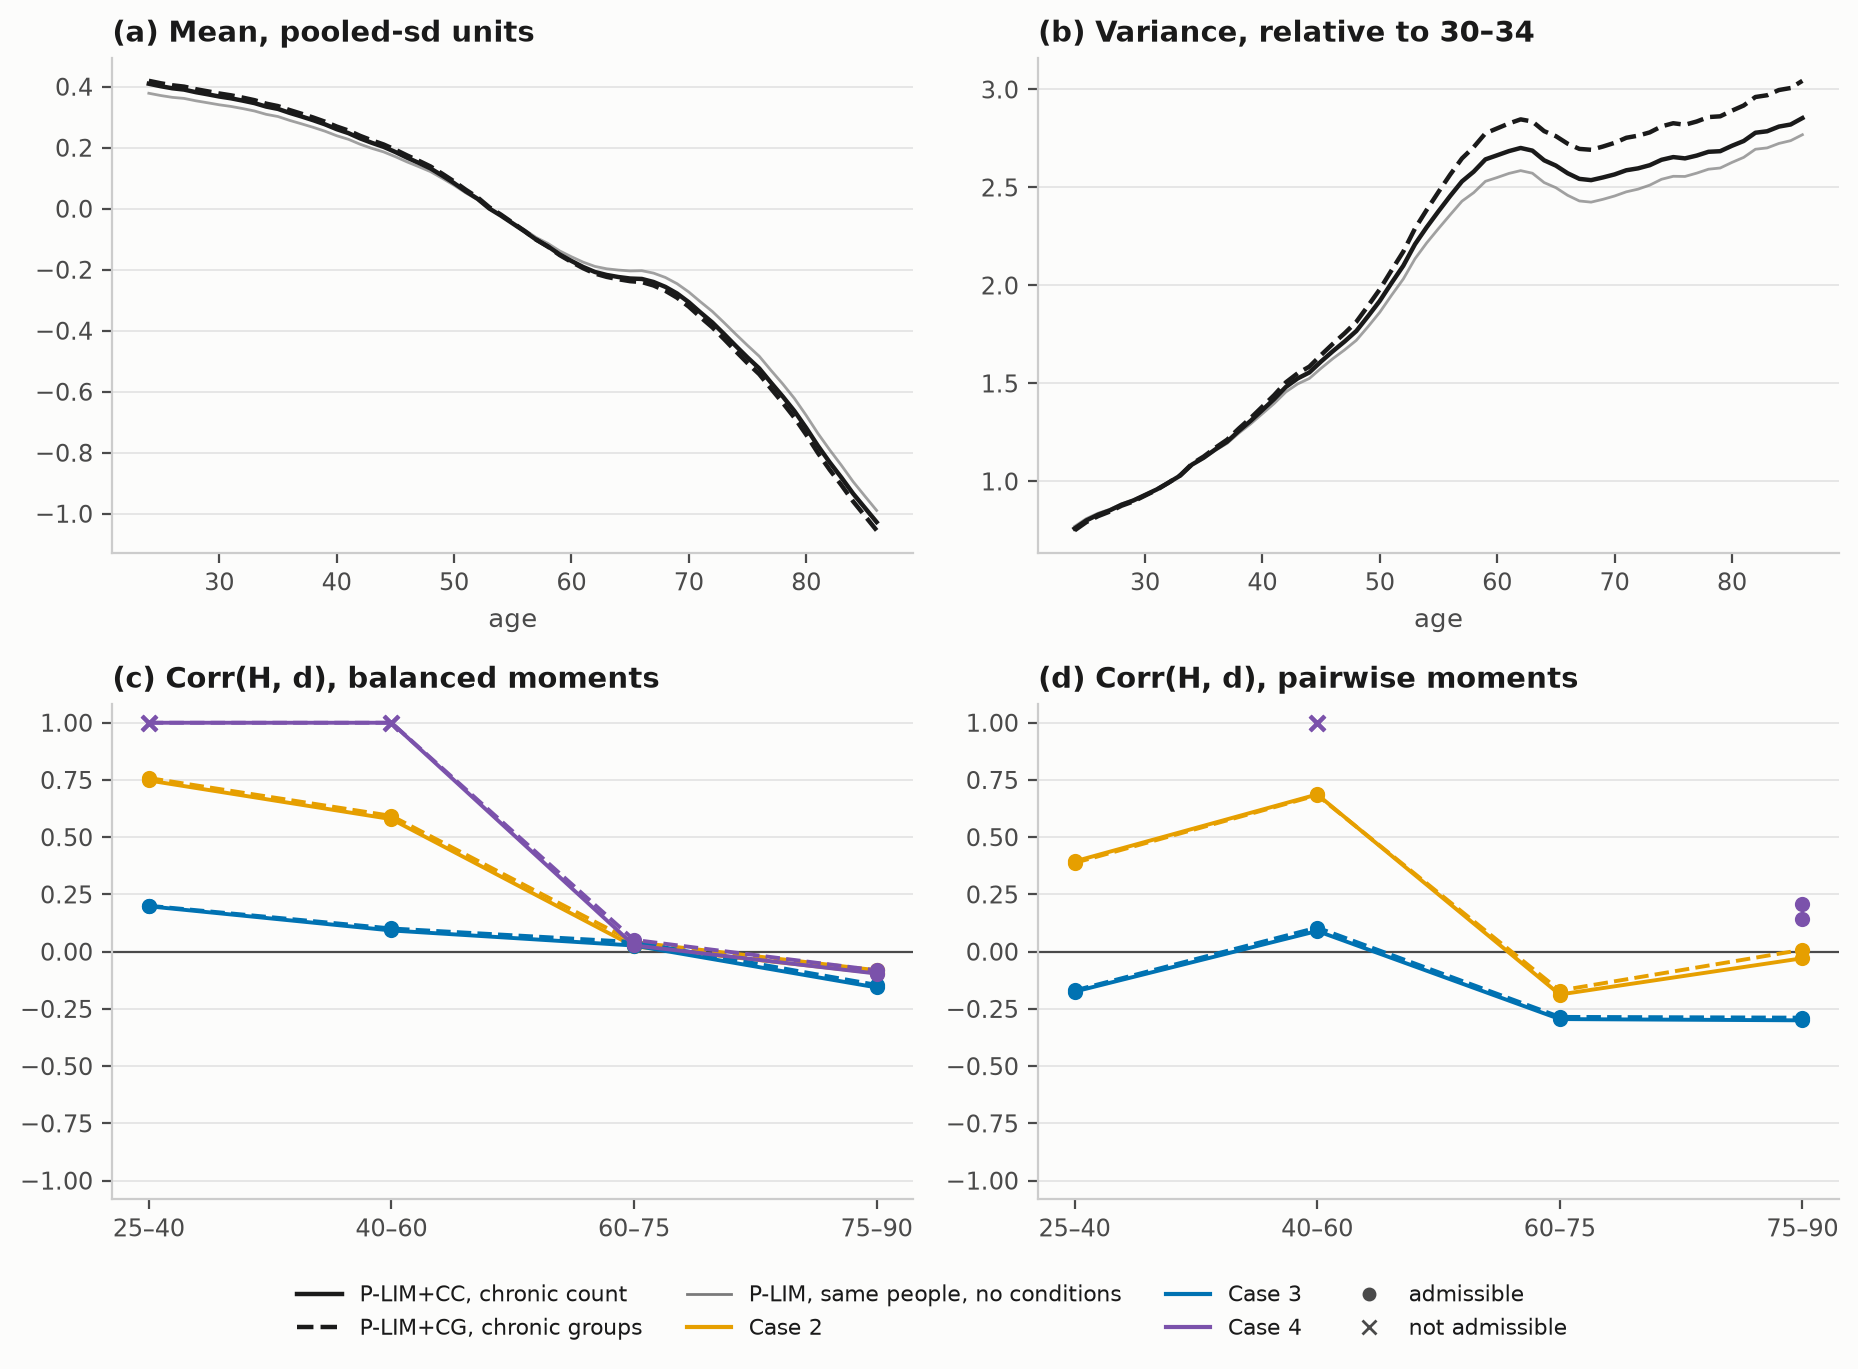
\includegraphics[width=\linewidth]{fig_con_exhibit1_plim}
\caption{Exhibit 1 for P-LIM+CC (solid) and P-LIM+CG (dashed) on $h$, as
Figure~\ref{fig:lim_ex1_pfunc}; grey lines are P-LIM without conditions on the
same people.}
\label{fig:con_ex1_plim}
\end{figure}

\begin{figure}[H]
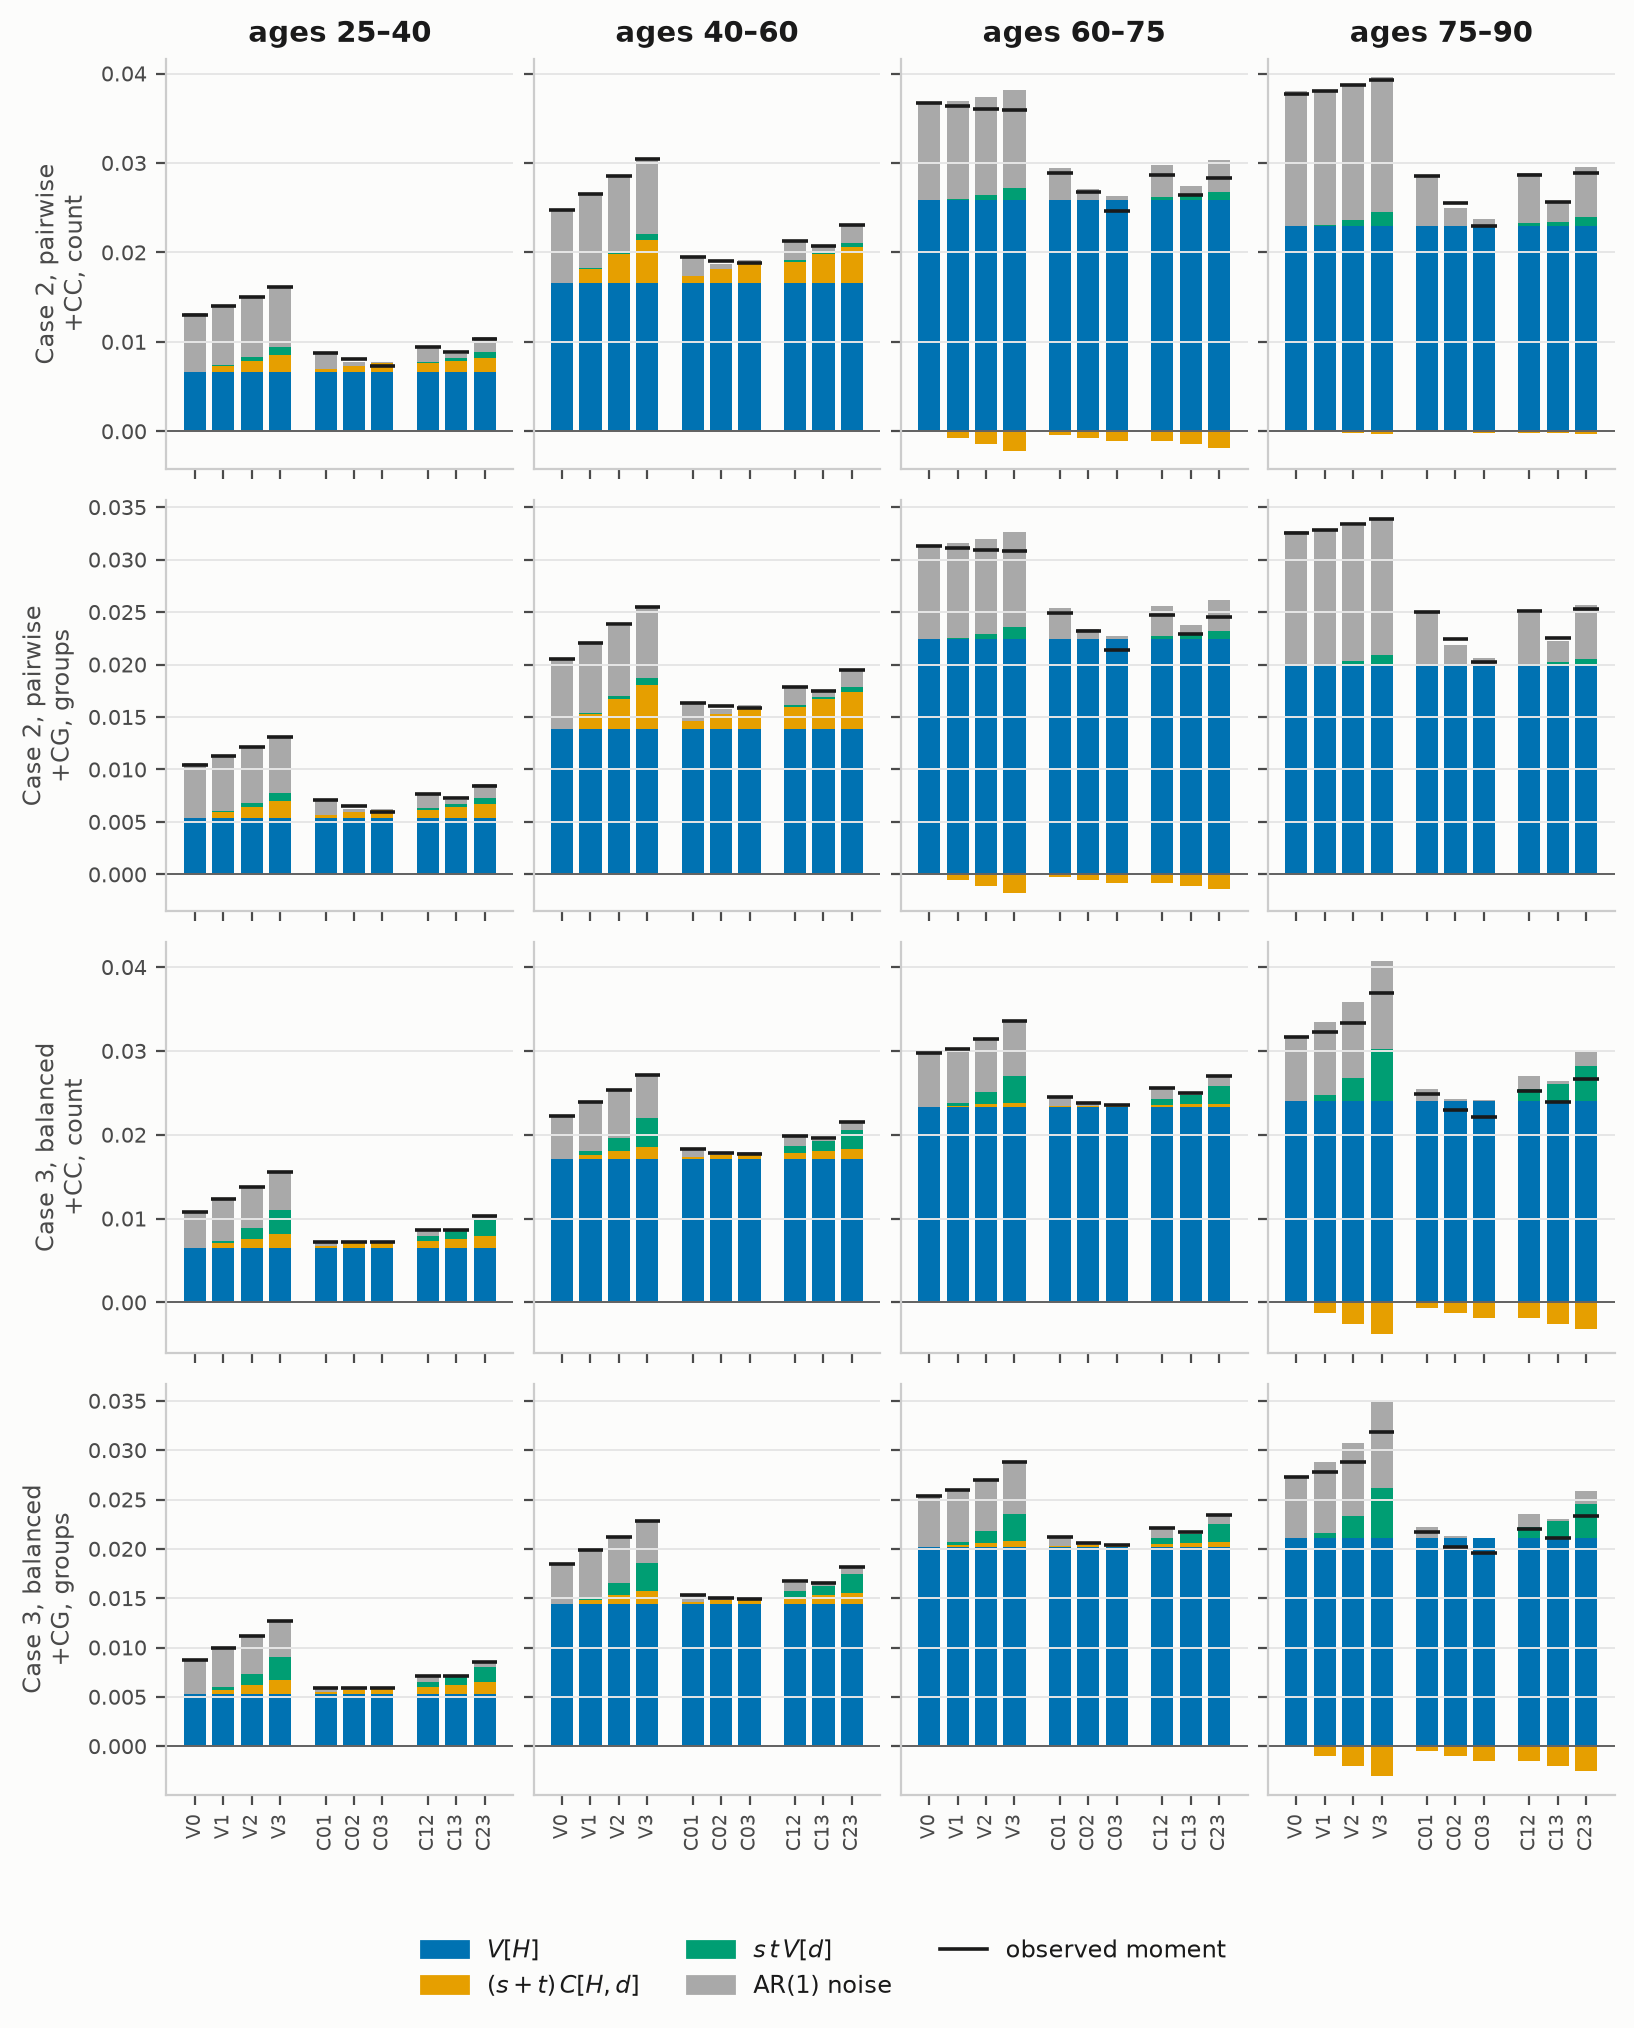
\includegraphics[width=\linewidth]{fig_con_bars_plim}
\caption{Identification barcharts for P-LIM+CC and P-LIM+CG on $h$, as
Figure~\ref{fig:lim_bars_pfunc}.}
\label{fig:con_bars_plim}
\end{figure}

\begin{figure}[H]
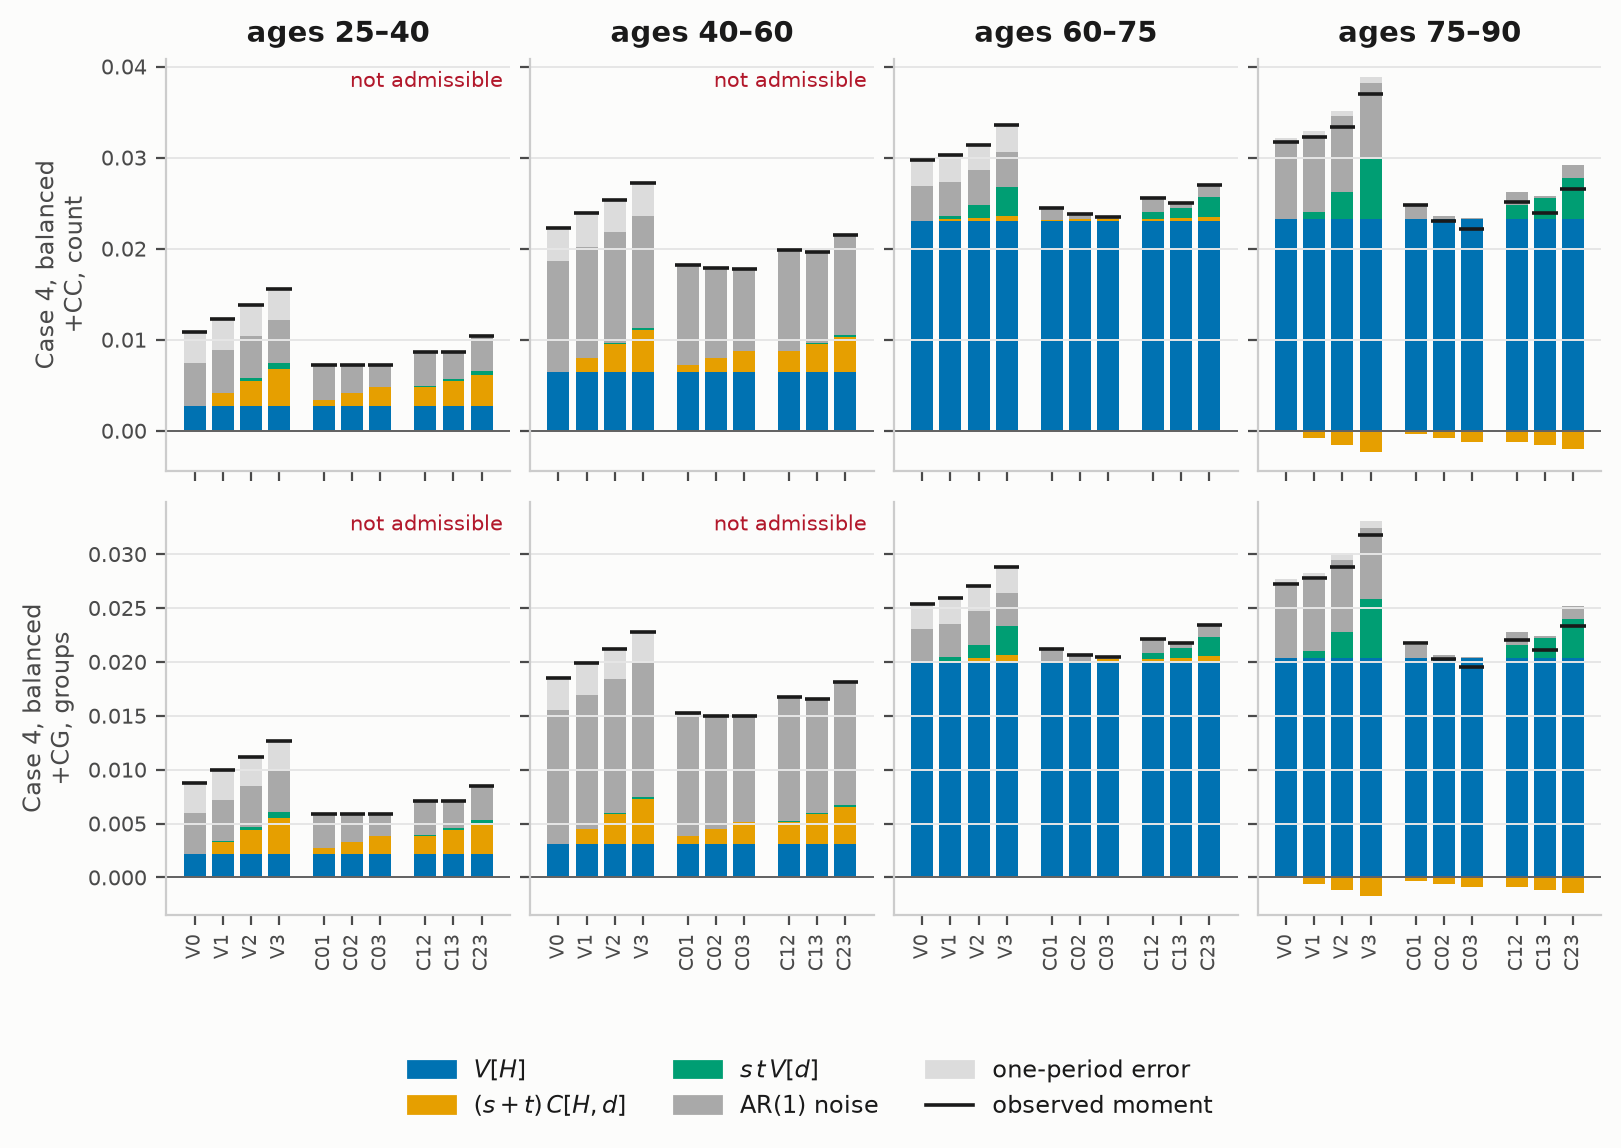
\includegraphics[width=\linewidth]{fig_con_bars_case4_plim}
\caption{Case 4 barcharts for P-LIM+CC and P-LIM+CG on $h$, as
Figure~\ref{fig:lim_bars4_pfunc}.}
\label{fig:con_bars4_plim}
\end{figure}

\begin{figure}[H]
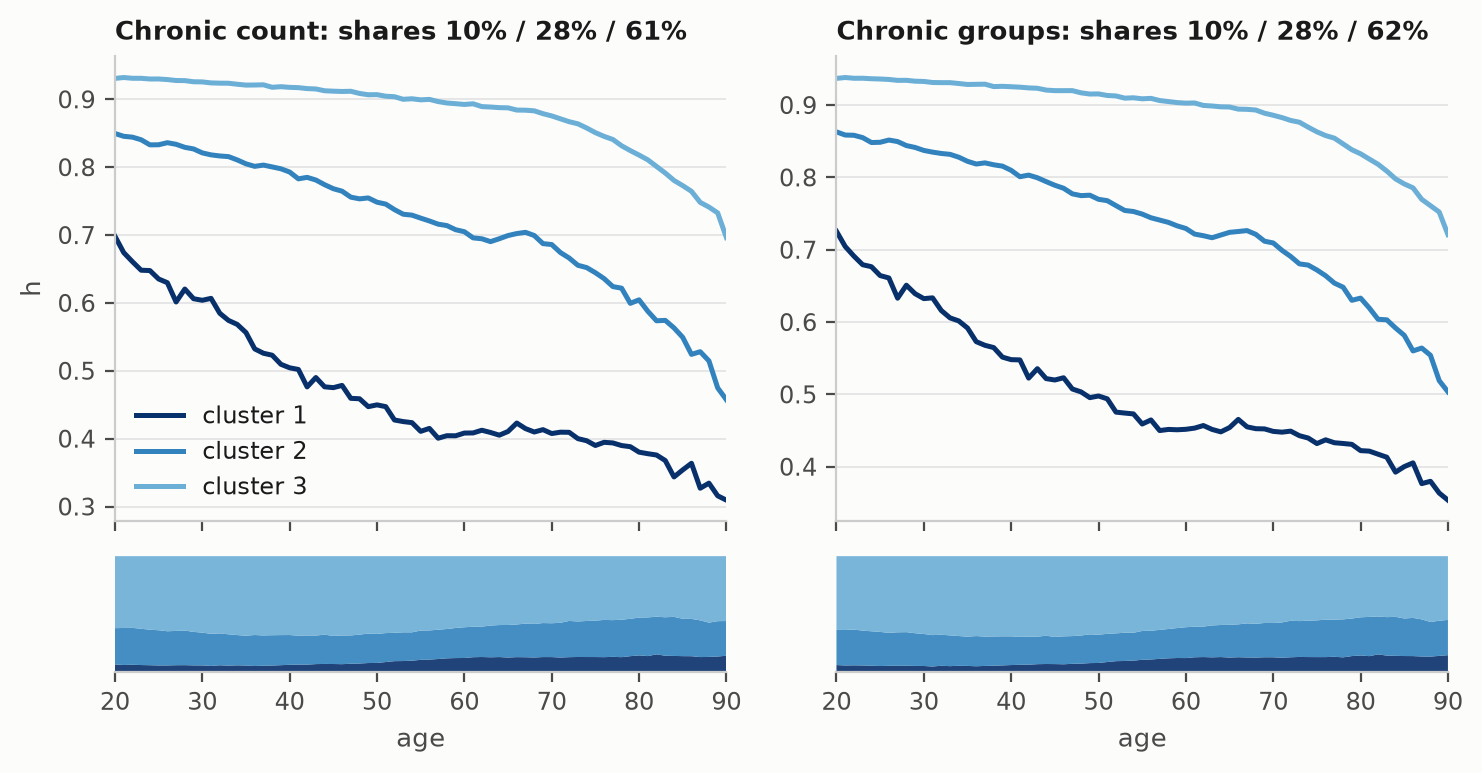
\includegraphics[width=\linewidth]{fig_con_clusters_plim}
\caption{Partial K-means, $K=3$, for P-LIM+CC (left) and P-LIM+CG (right) on $h$,
as Figure~\ref{fig:lim_cl_pfunc}.}
\label{fig:con_cl_plim}
\end{figure}

\subsubsection{P-LIM4 with conditions}

\begin{figure}[H]
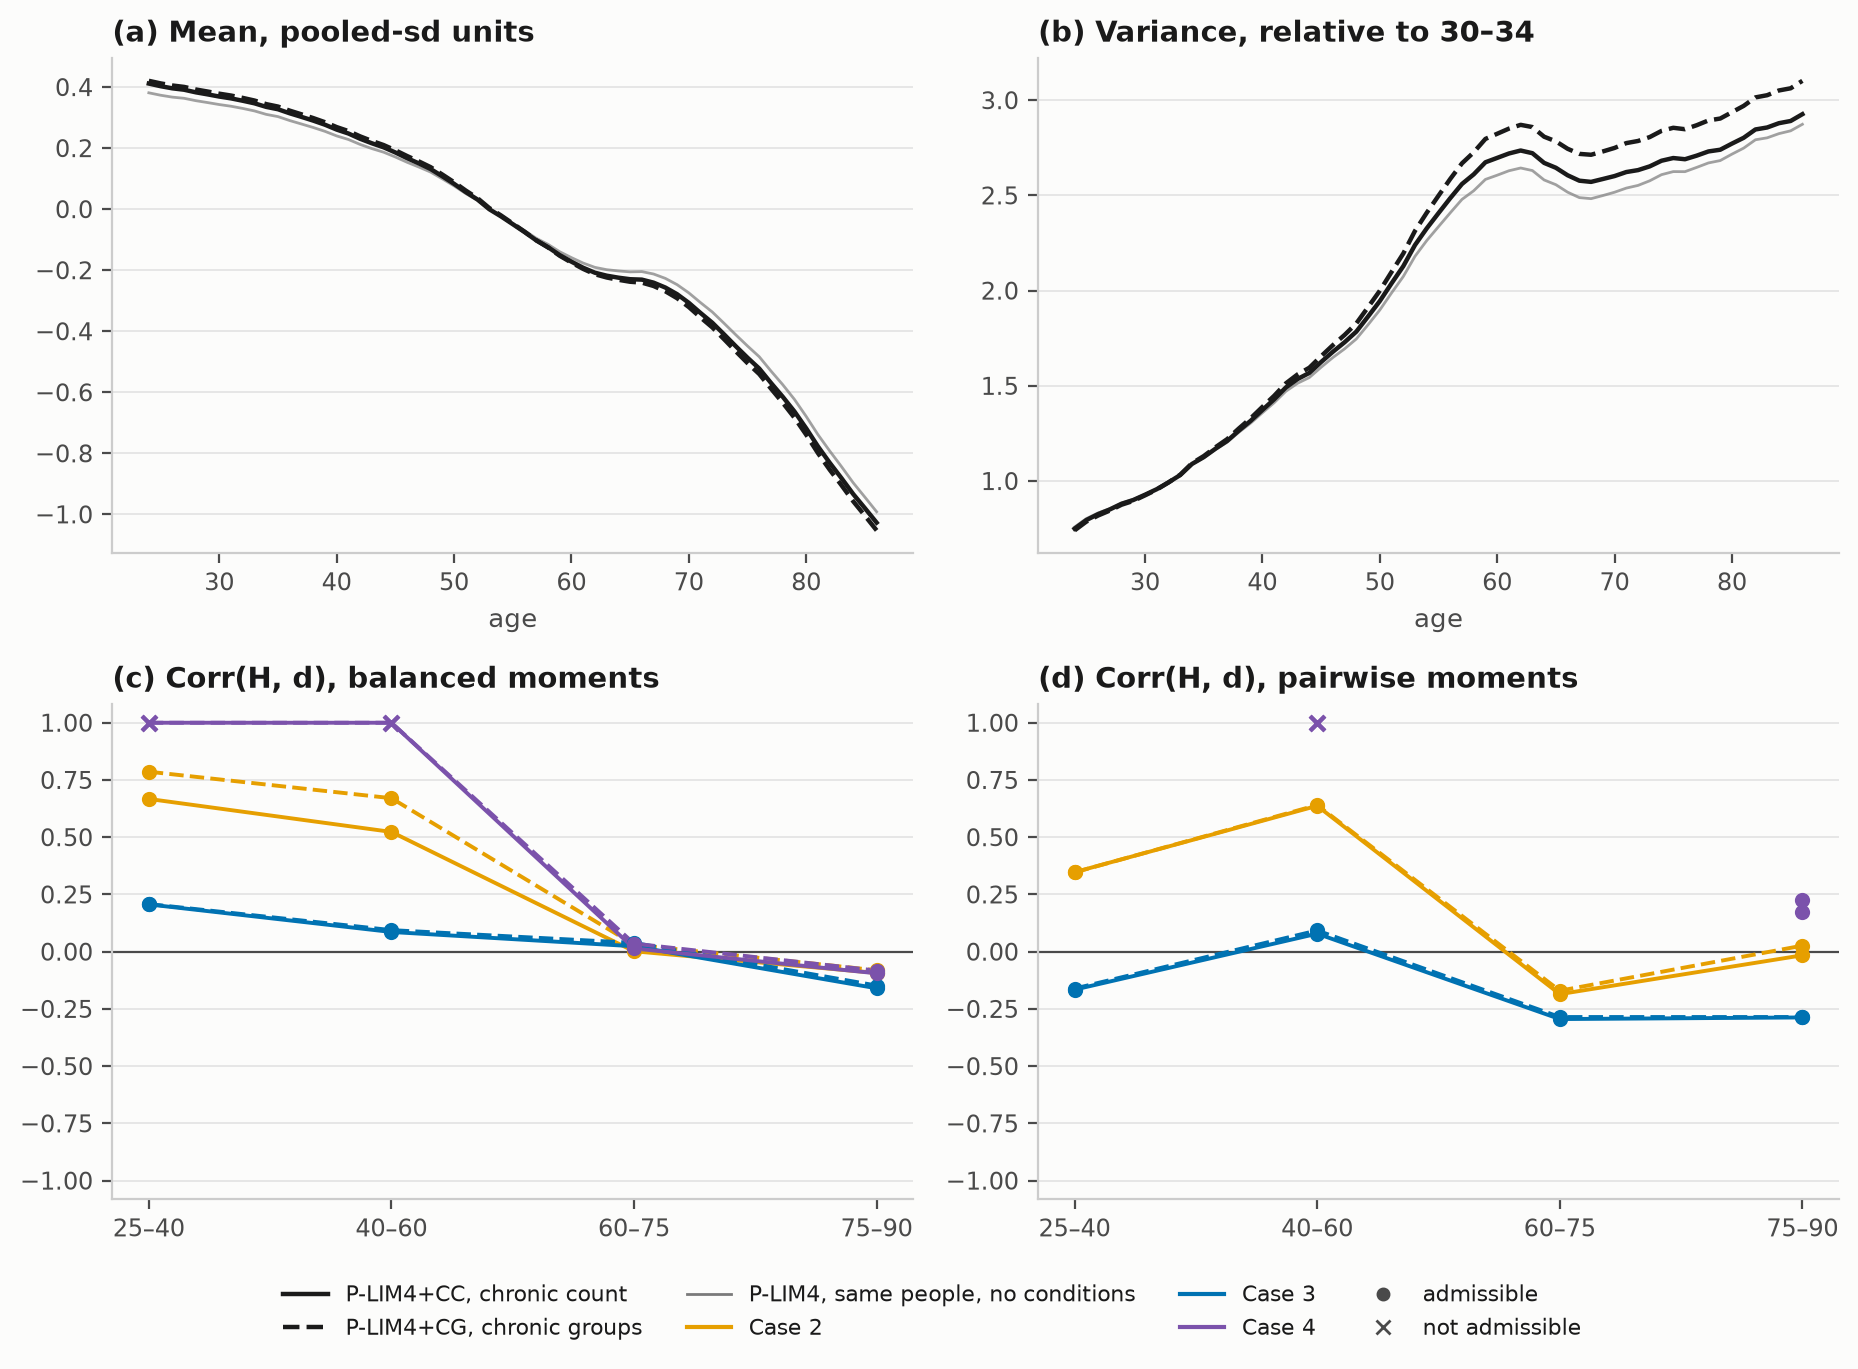
\includegraphics[width=\linewidth]{fig_con_exhibit1_plim4}
\caption{Exhibit 1 for P-LIM4+CC (solid) and P-LIM4+CG (dashed) on $h$, as
Figure~\ref{fig:lim_ex1_pfunc}; grey lines are P-LIM4 without conditions on the
same people.}
\label{fig:con_ex1_plim4}
\end{figure}

\begin{figure}[H]
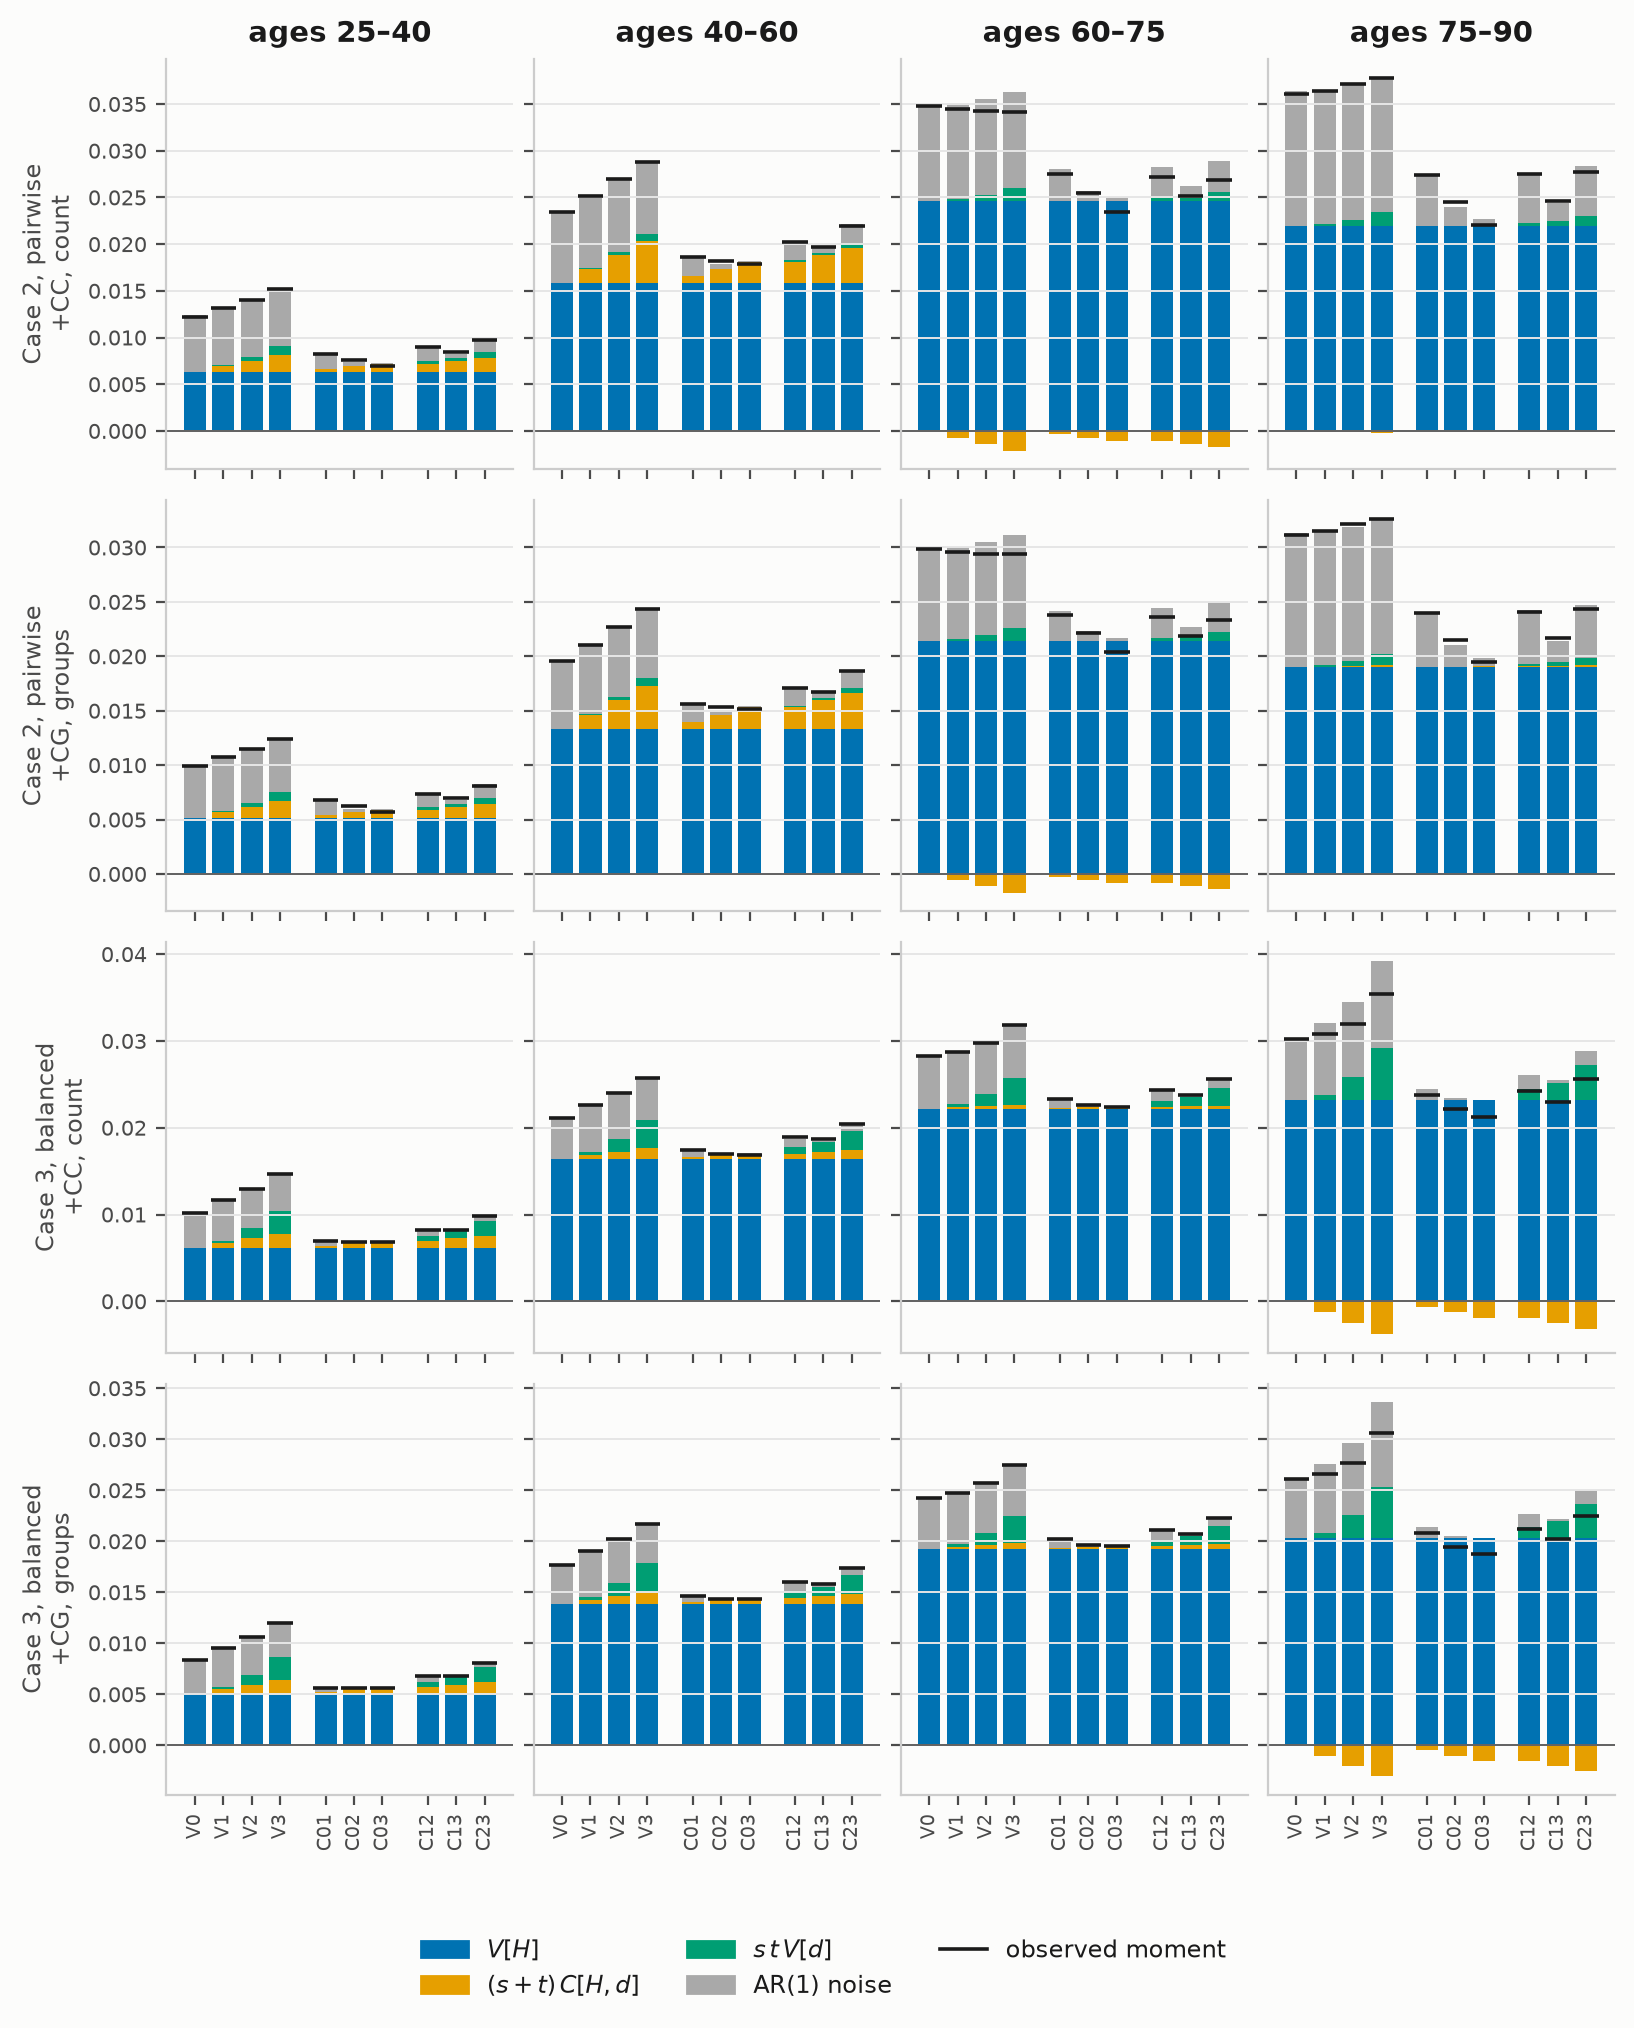
\includegraphics[width=\linewidth]{fig_con_bars_plim4}
\caption{Identification barcharts for P-LIM4+CC and P-LIM4+CG on $h$, as
Figure~\ref{fig:lim_bars_pfunc}.}
\label{fig:con_bars_plim4}
\end{figure}

\begin{figure}[H]
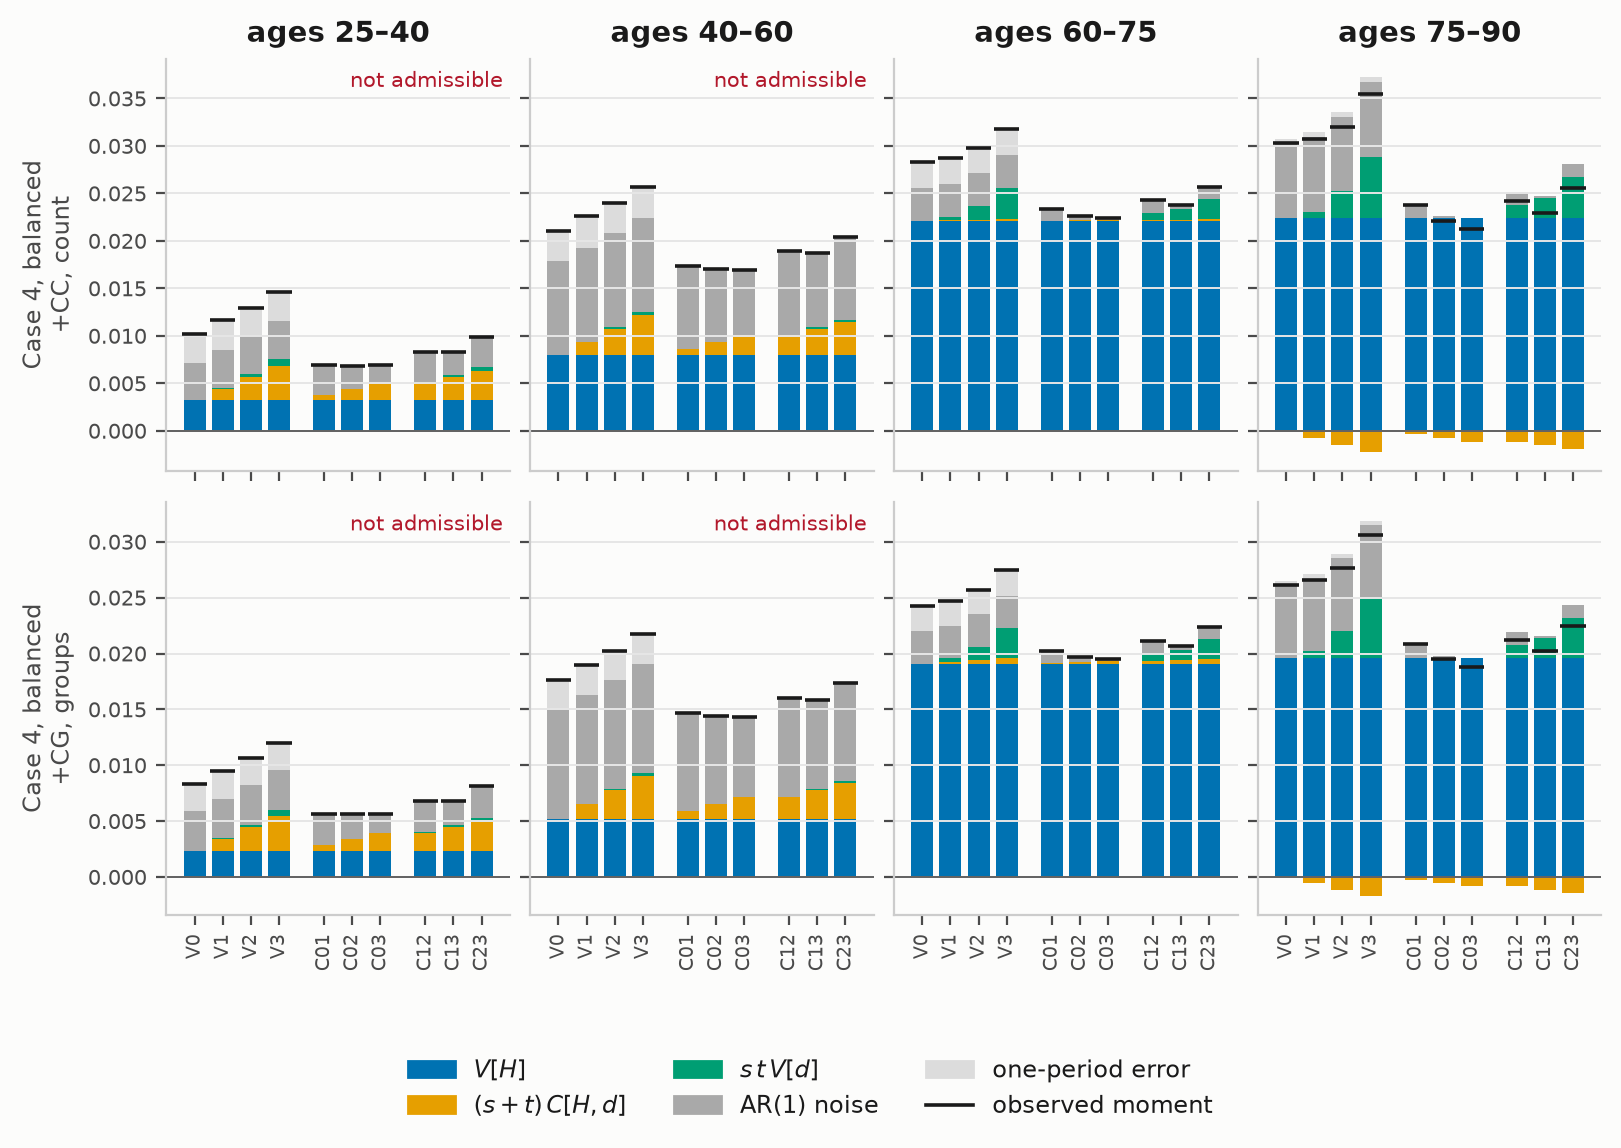
\includegraphics[width=\linewidth]{fig_con_bars_case4_plim4}
\caption{Case 4 barcharts for P-LIM4+CC and P-LIM4+CG on $h$, as
Figure~\ref{fig:lim_bars4_pfunc}.}
\label{fig:con_bars4_plim4}
\end{figure}

\begin{figure}[H]
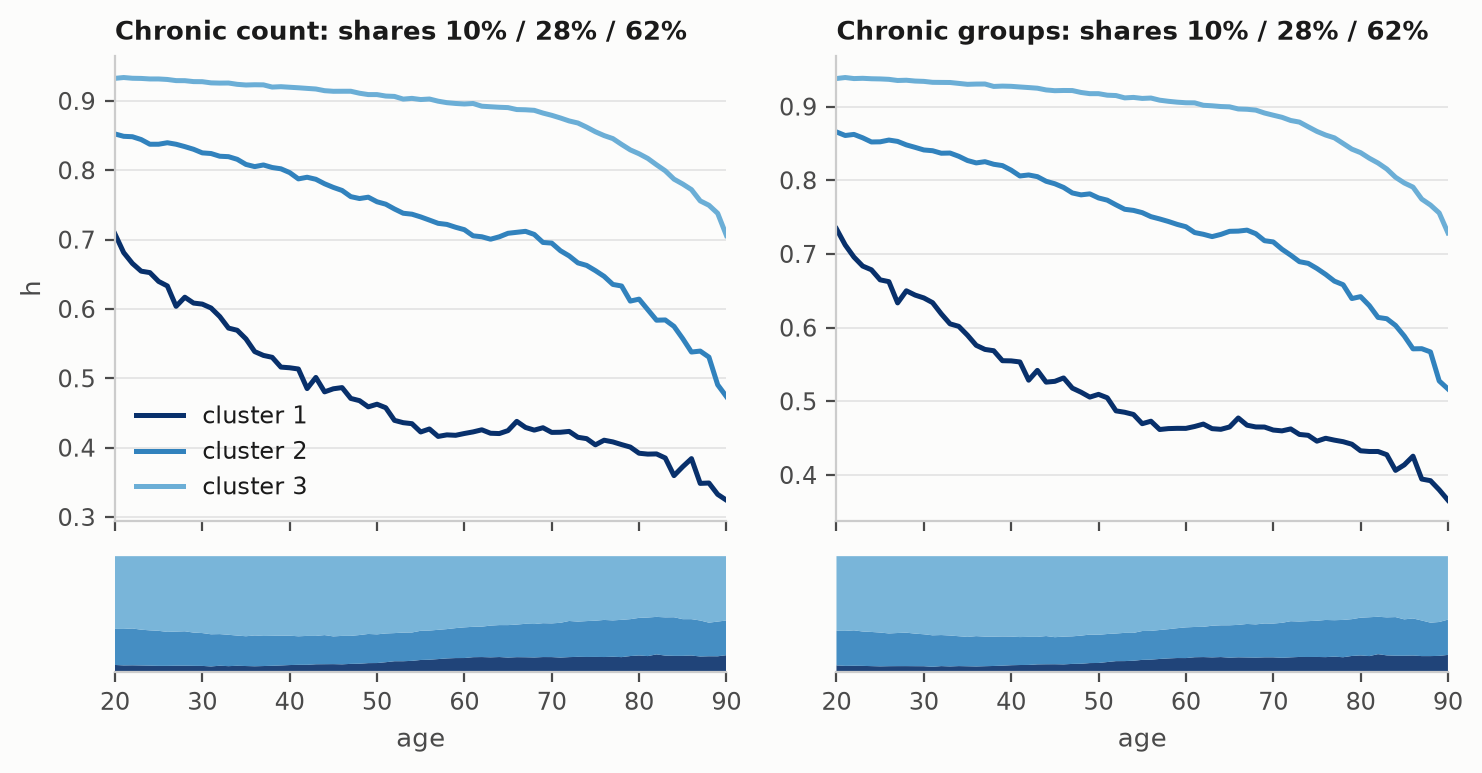
\includegraphics[width=\linewidth]{fig_con_clusters_plim4}
\caption{Partial K-means, $K=3$, for P-LIM4+CC (left) and P-LIM4+CG (right) on $h$,
as Figure~\ref{fig:lim_cl_pfunc}.}
\label{fig:con_cl_plim4}
\end{figure}

\subsubsection{P-LIM3 with conditions}

\begin{figure}[H]
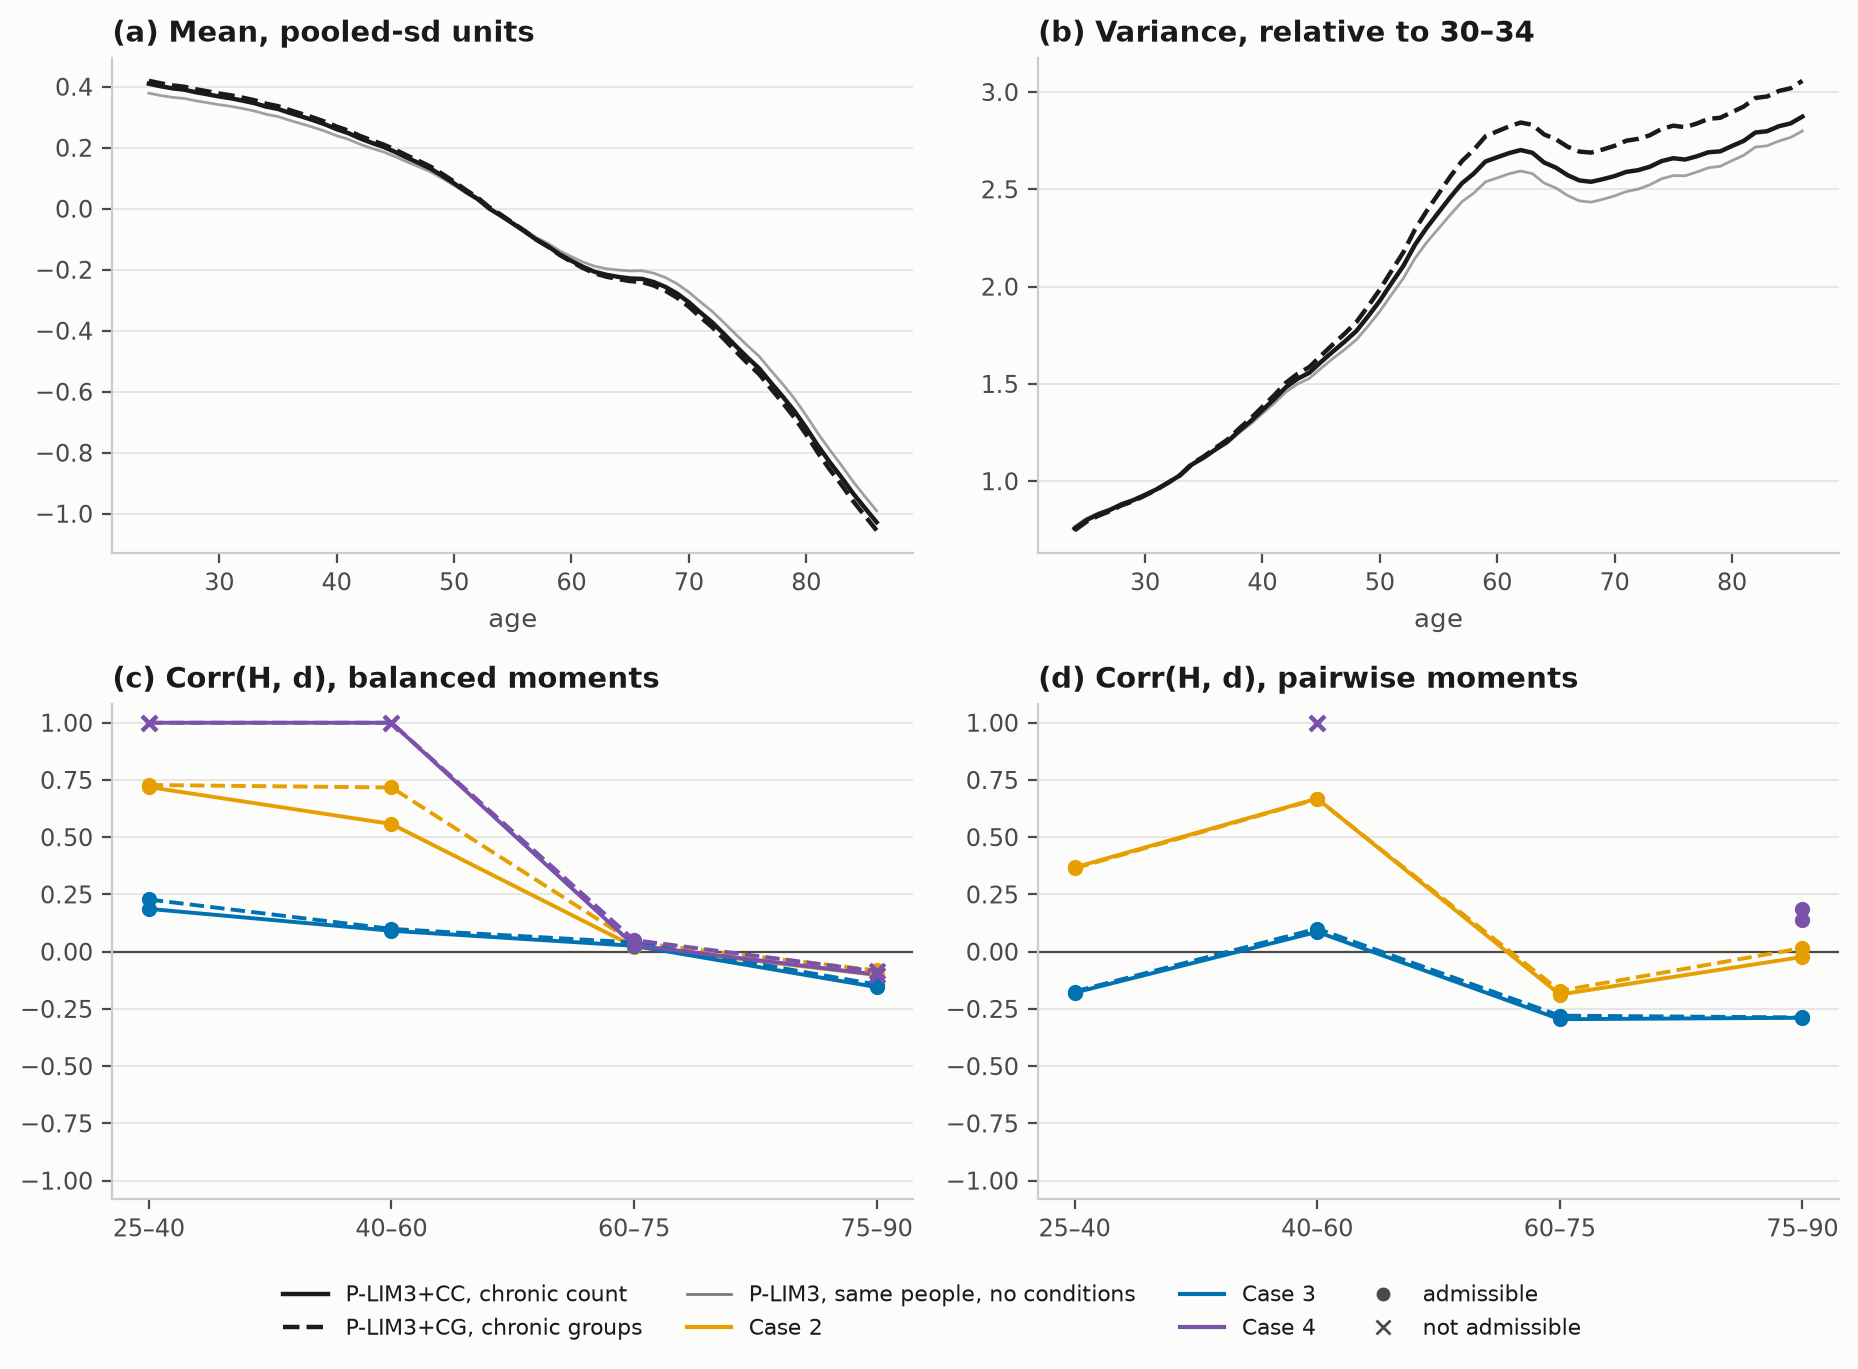
\includegraphics[width=\linewidth]{fig_con_exhibit1_plim3}
\caption{Exhibit 1 for P-LIM3+CC (solid) and P-LIM3+CG (dashed) on $h$, as
Figure~\ref{fig:lim_ex1_pfunc}; grey lines are P-LIM3 without conditions on the
same people.}
\label{fig:con_ex1_plim3}
\end{figure}

\begin{figure}[H]
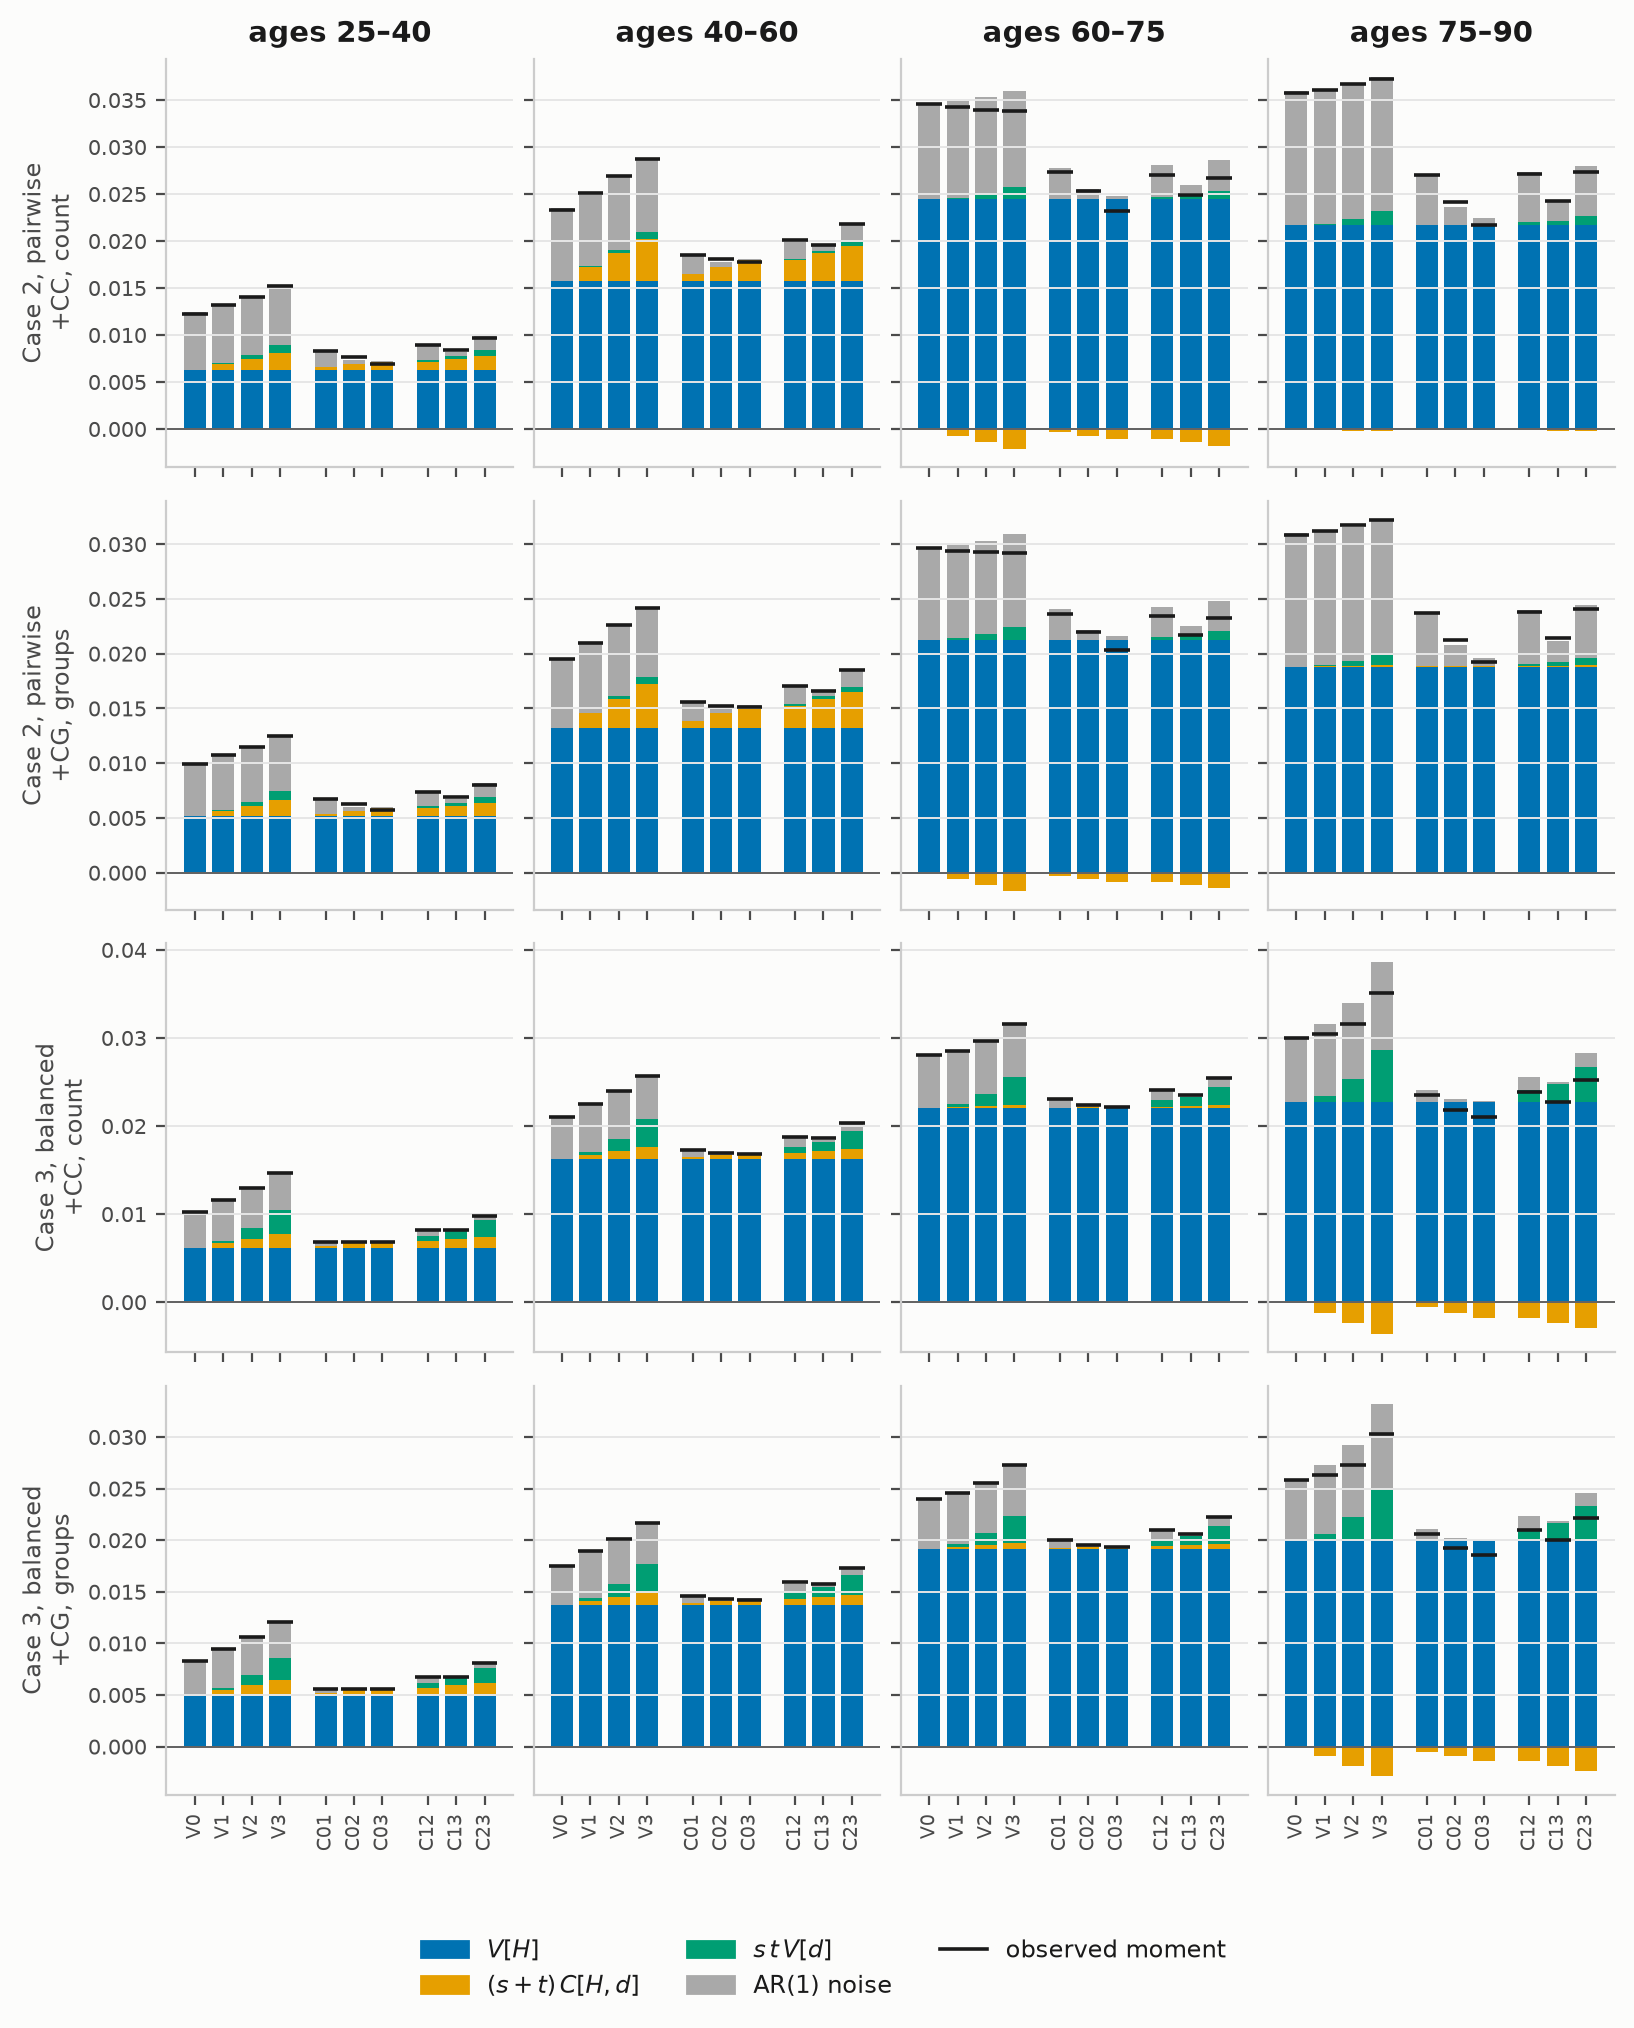
\includegraphics[width=\linewidth]{fig_con_bars_plim3}
\caption{Identification barcharts for P-LIM3+CC and P-LIM3+CG on $h$, as
Figure~\ref{fig:lim_bars_pfunc}.}
\label{fig:con_bars_plim3}
\end{figure}

\begin{figure}[H]
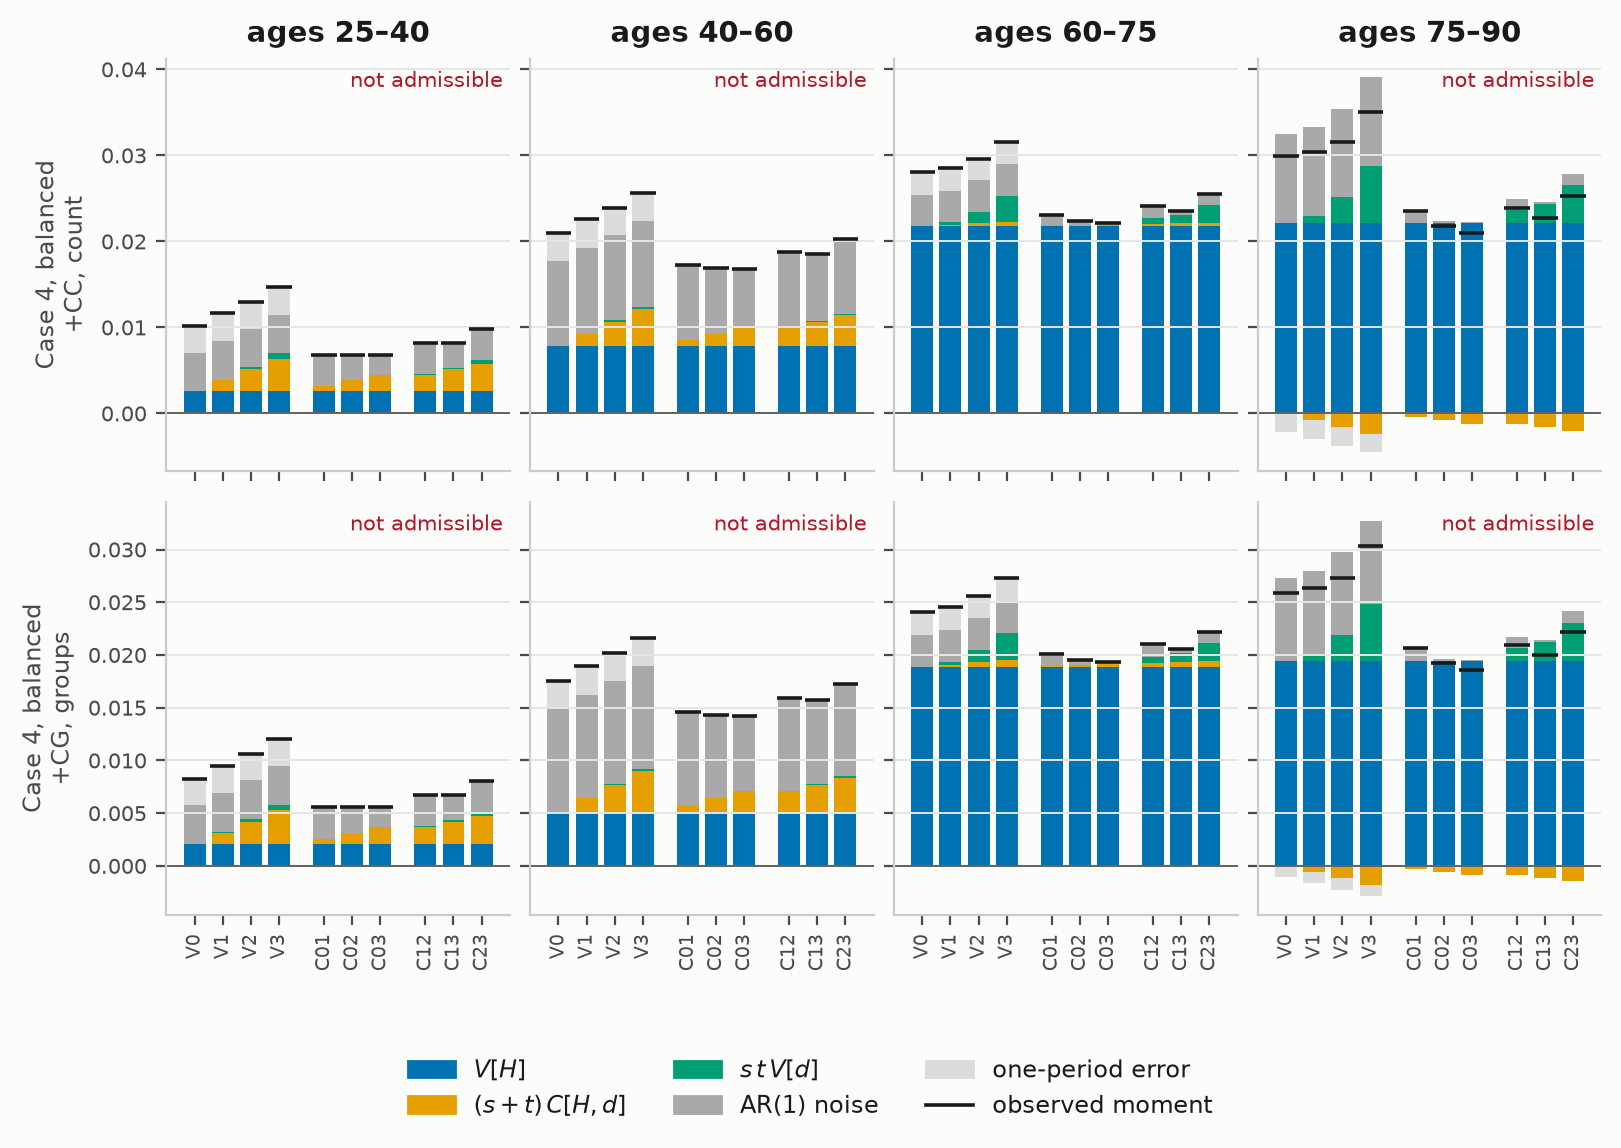
\includegraphics[width=\linewidth]{fig_con_bars_case4_plim3}
\caption{Case 4 barcharts for P-LIM3+CC and P-LIM3+CG on $h$, as
Figure~\ref{fig:lim_bars4_pfunc}.}
\label{fig:con_bars4_plim3}
\end{figure}

\begin{figure}[H]
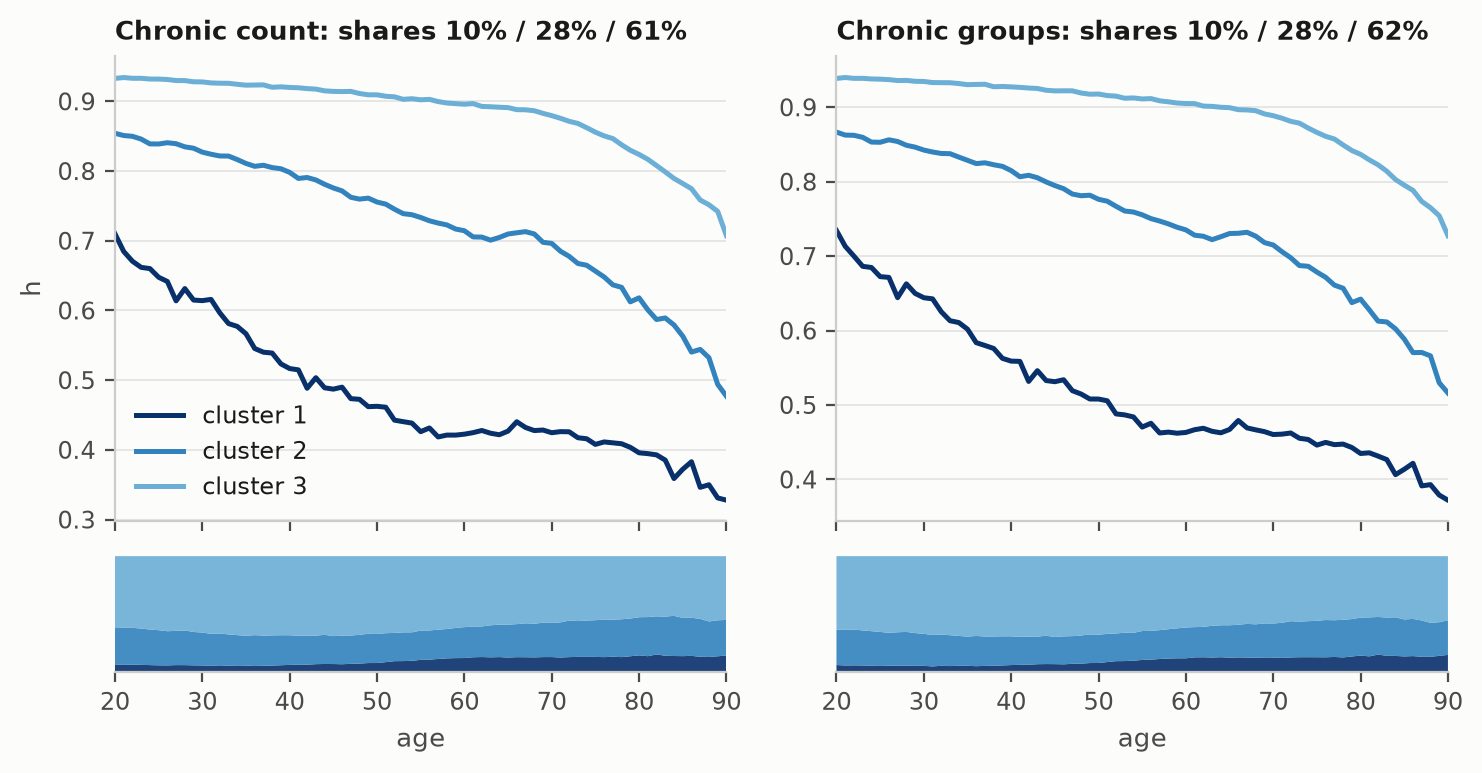
\includegraphics[width=\linewidth]{fig_con_clusters_plim3}
\caption{Partial K-means, $K=3$, for P-LIM3+CC (left) and P-LIM3+CG (right) on $h$,
as Figure~\ref{fig:lim_cl_pfunc}.}
\label{fig:con_cl_plim3}
\end{figure}

\subsubsection{P-LIM3+O with conditions}

\begin{figure}[H]
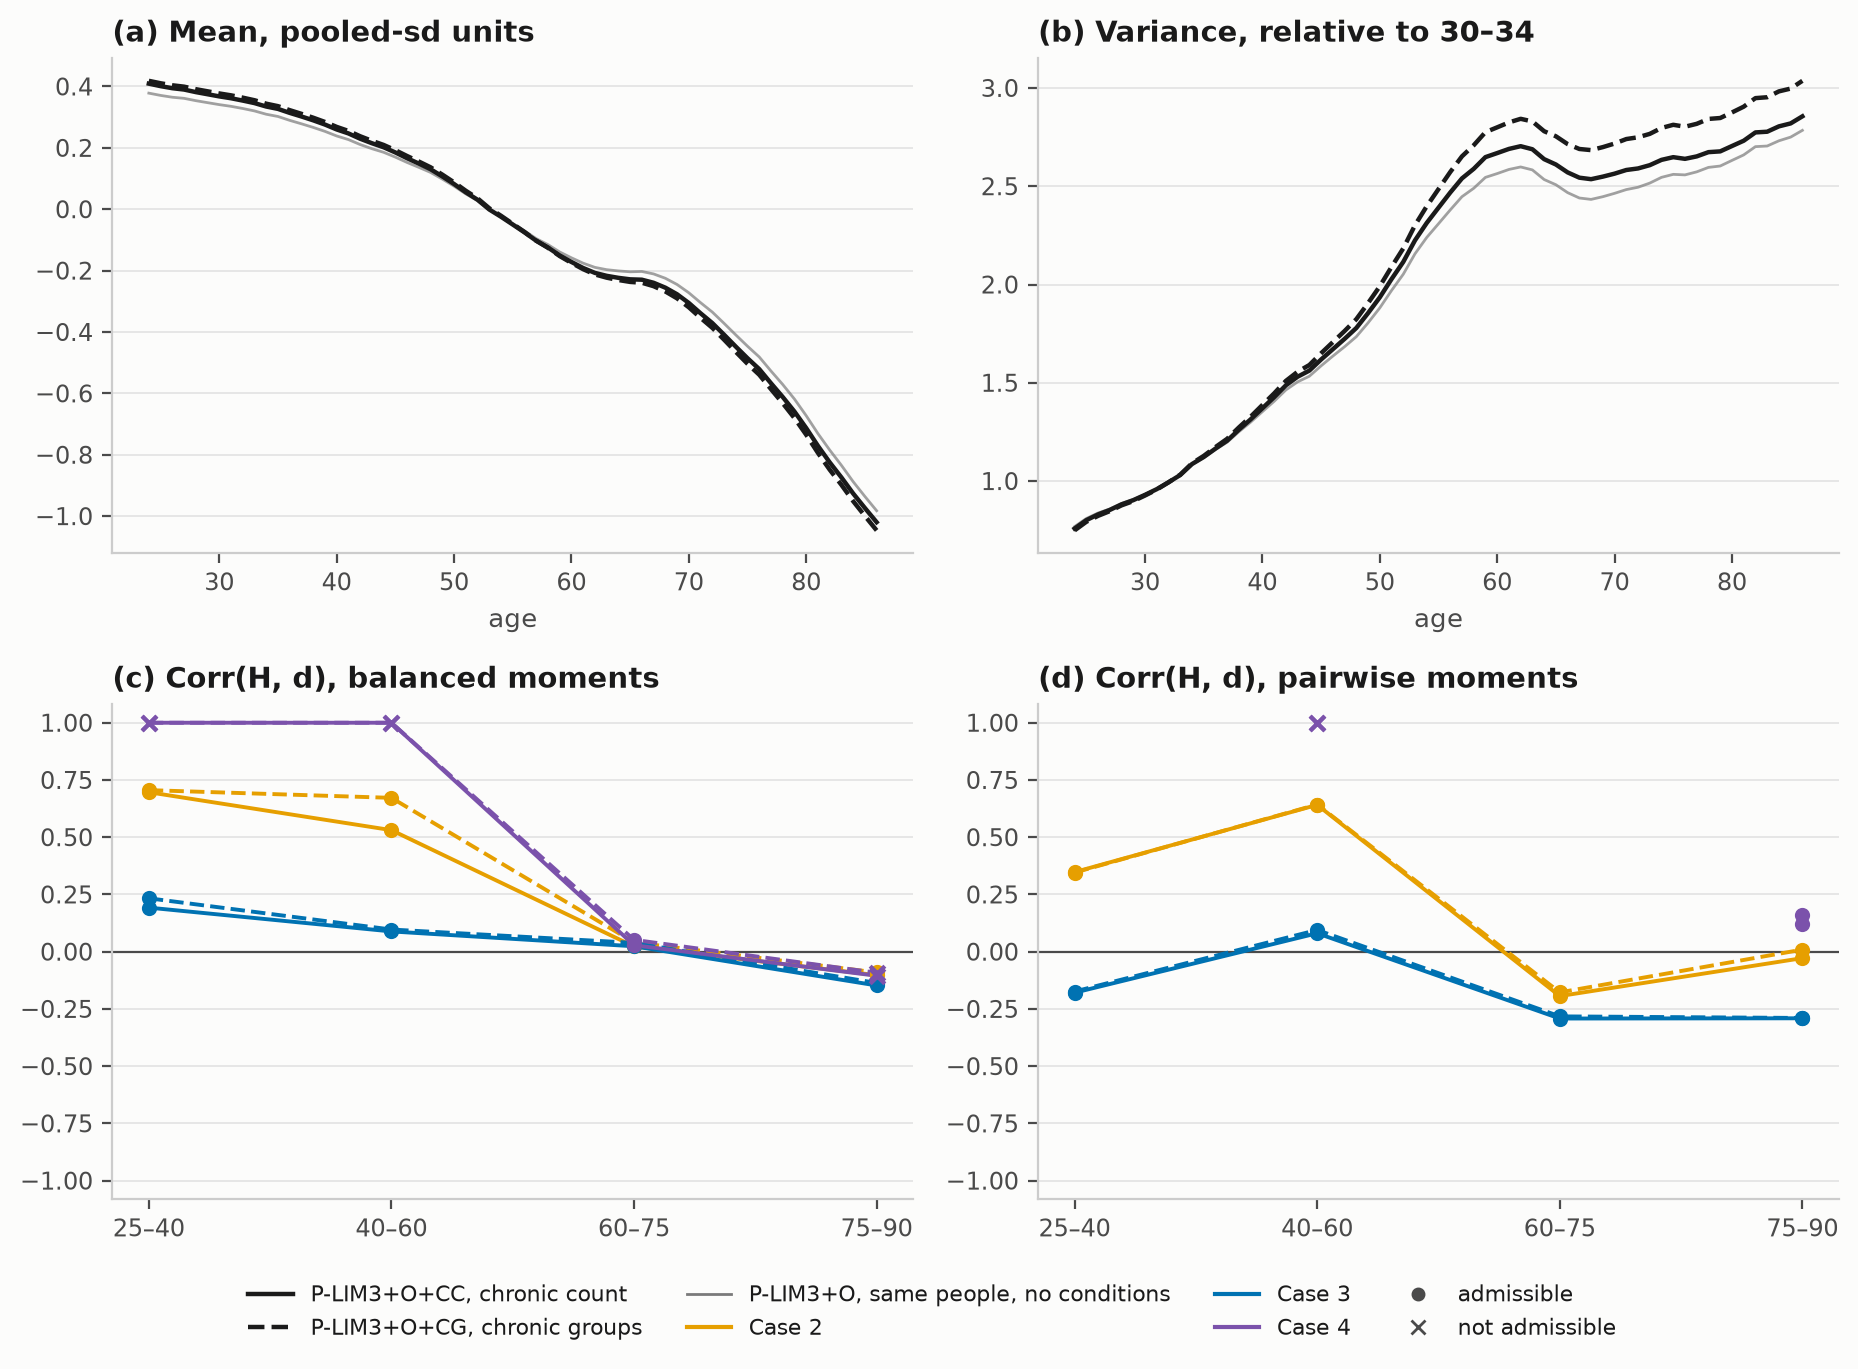
\includegraphics[width=\linewidth]{fig_con_exhibit1_plim3o}
\caption{Exhibit 1 for P-LIM3+O+CC (solid) and P-LIM3+O+CG (dashed) on $h$, as
Figure~\ref{fig:lim_ex1_pfunc}; grey lines are P-LIM3+O without conditions on the
same people.}
\label{fig:con_ex1_plim3o}
\end{figure}

\begin{figure}[H]
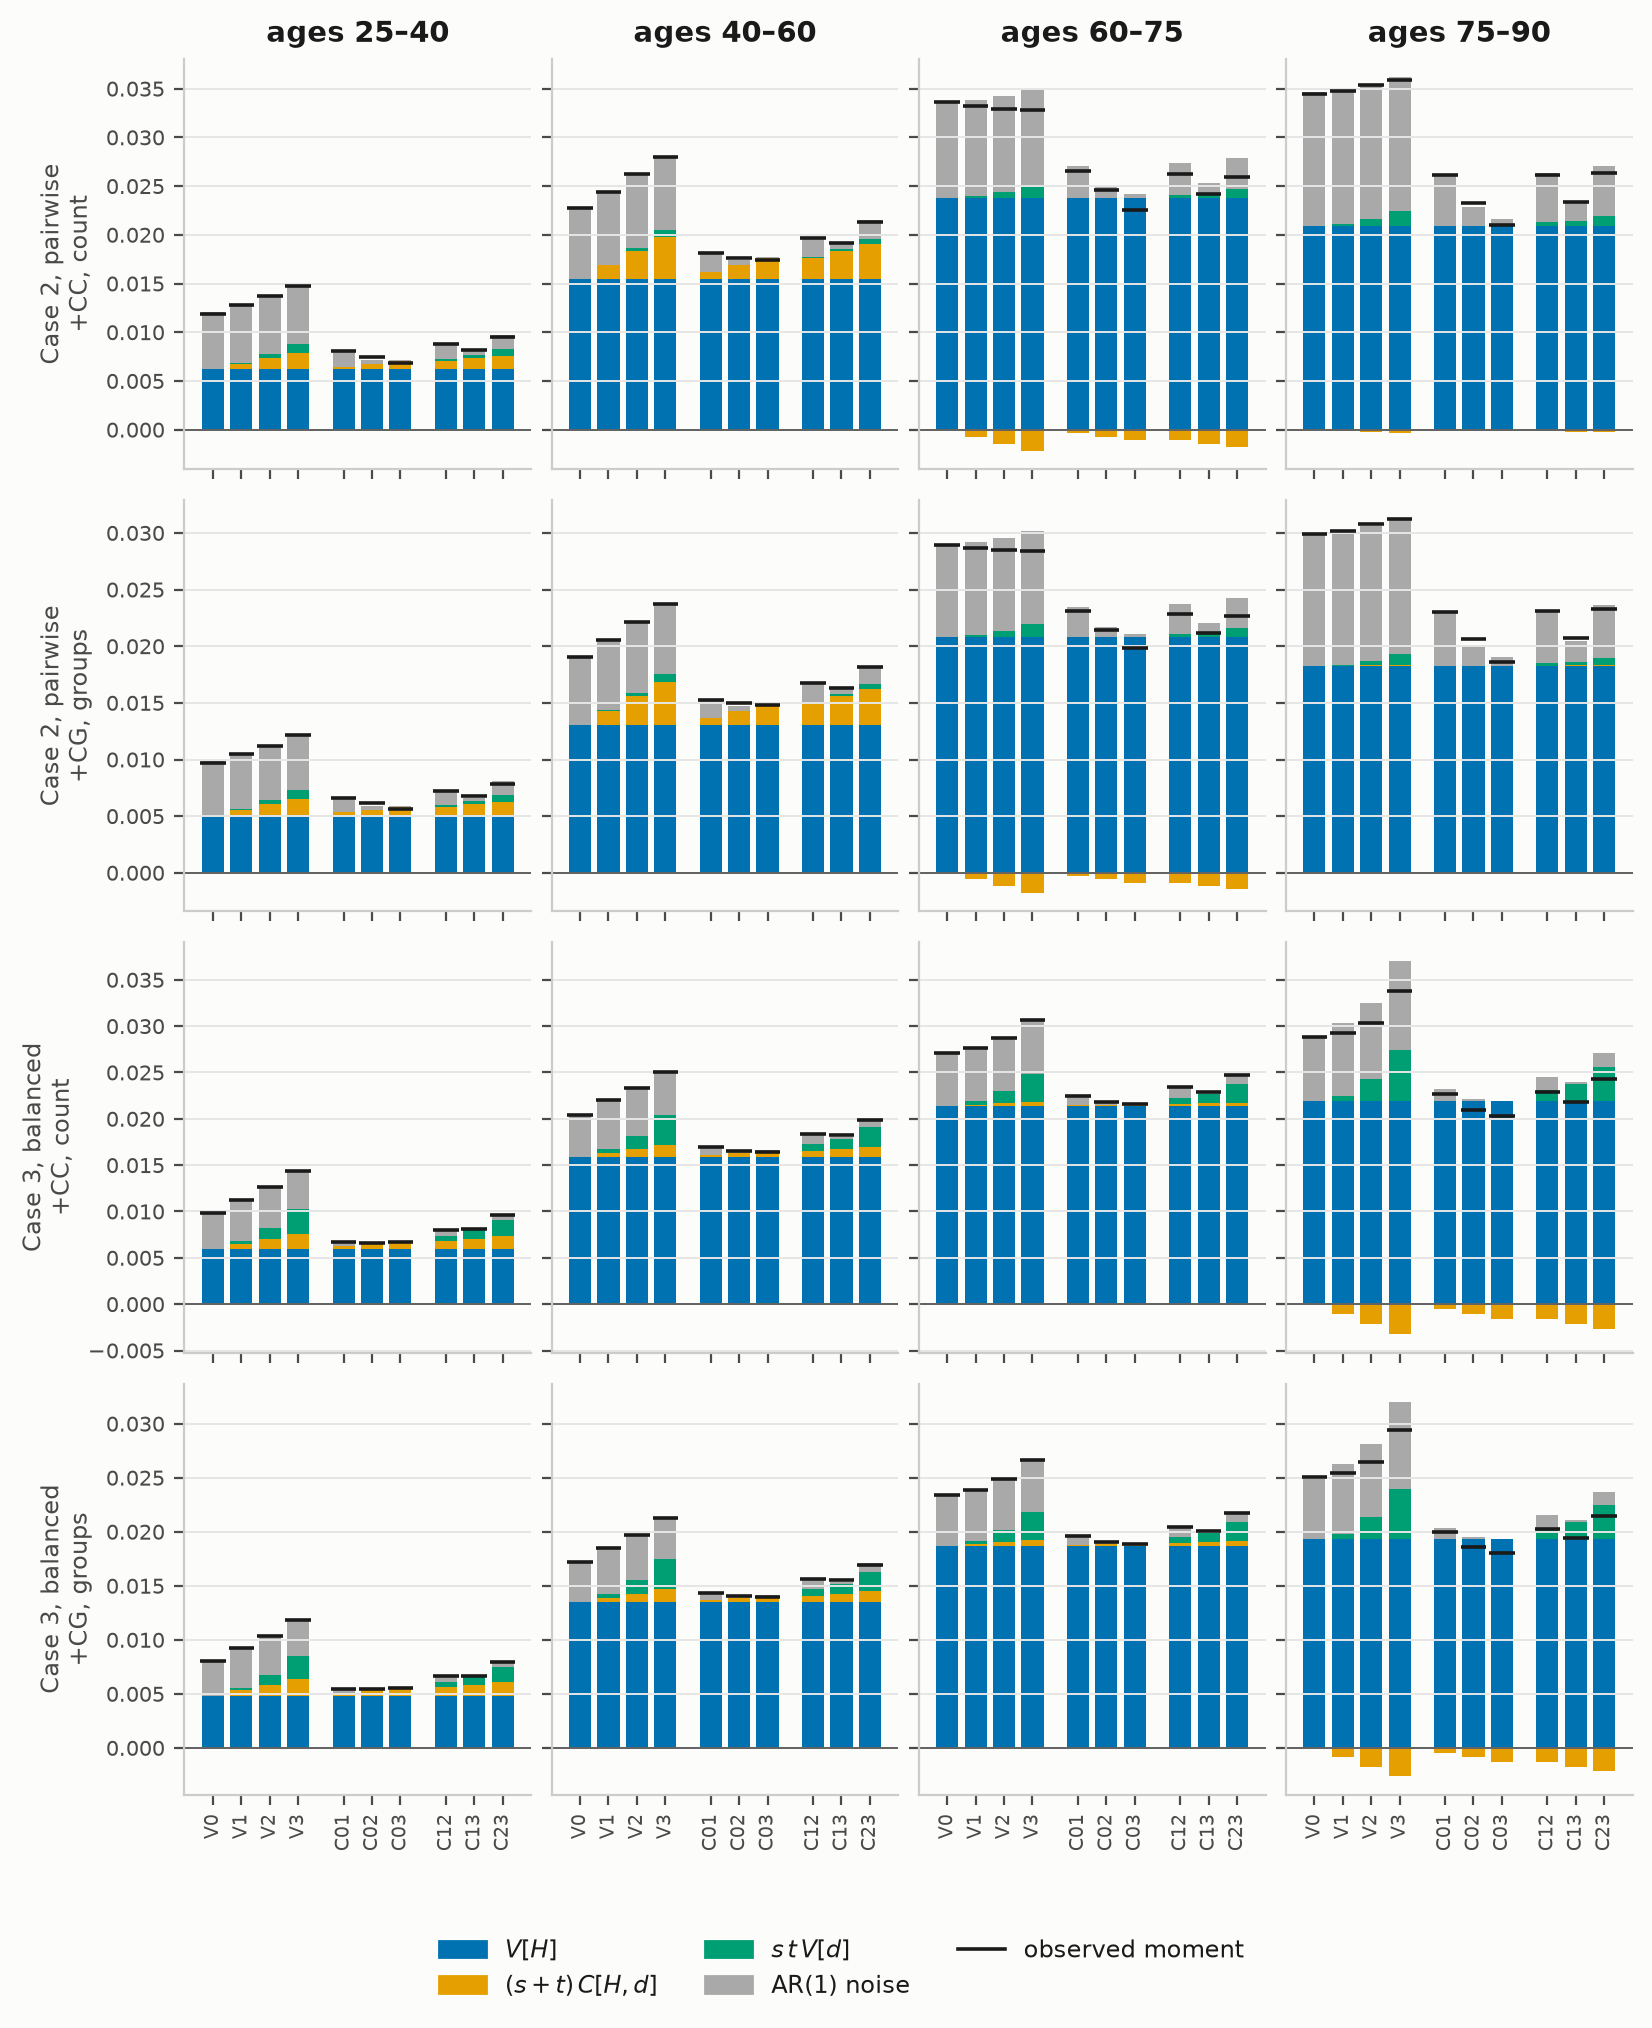
\includegraphics[width=\linewidth]{fig_con_bars_plim3o}
\caption{Identification barcharts for P-LIM3+O+CC and P-LIM3+O+CG on $h$, as
Figure~\ref{fig:lim_bars_pfunc}.}
\label{fig:con_bars_plim3o}
\end{figure}

\begin{figure}[H]
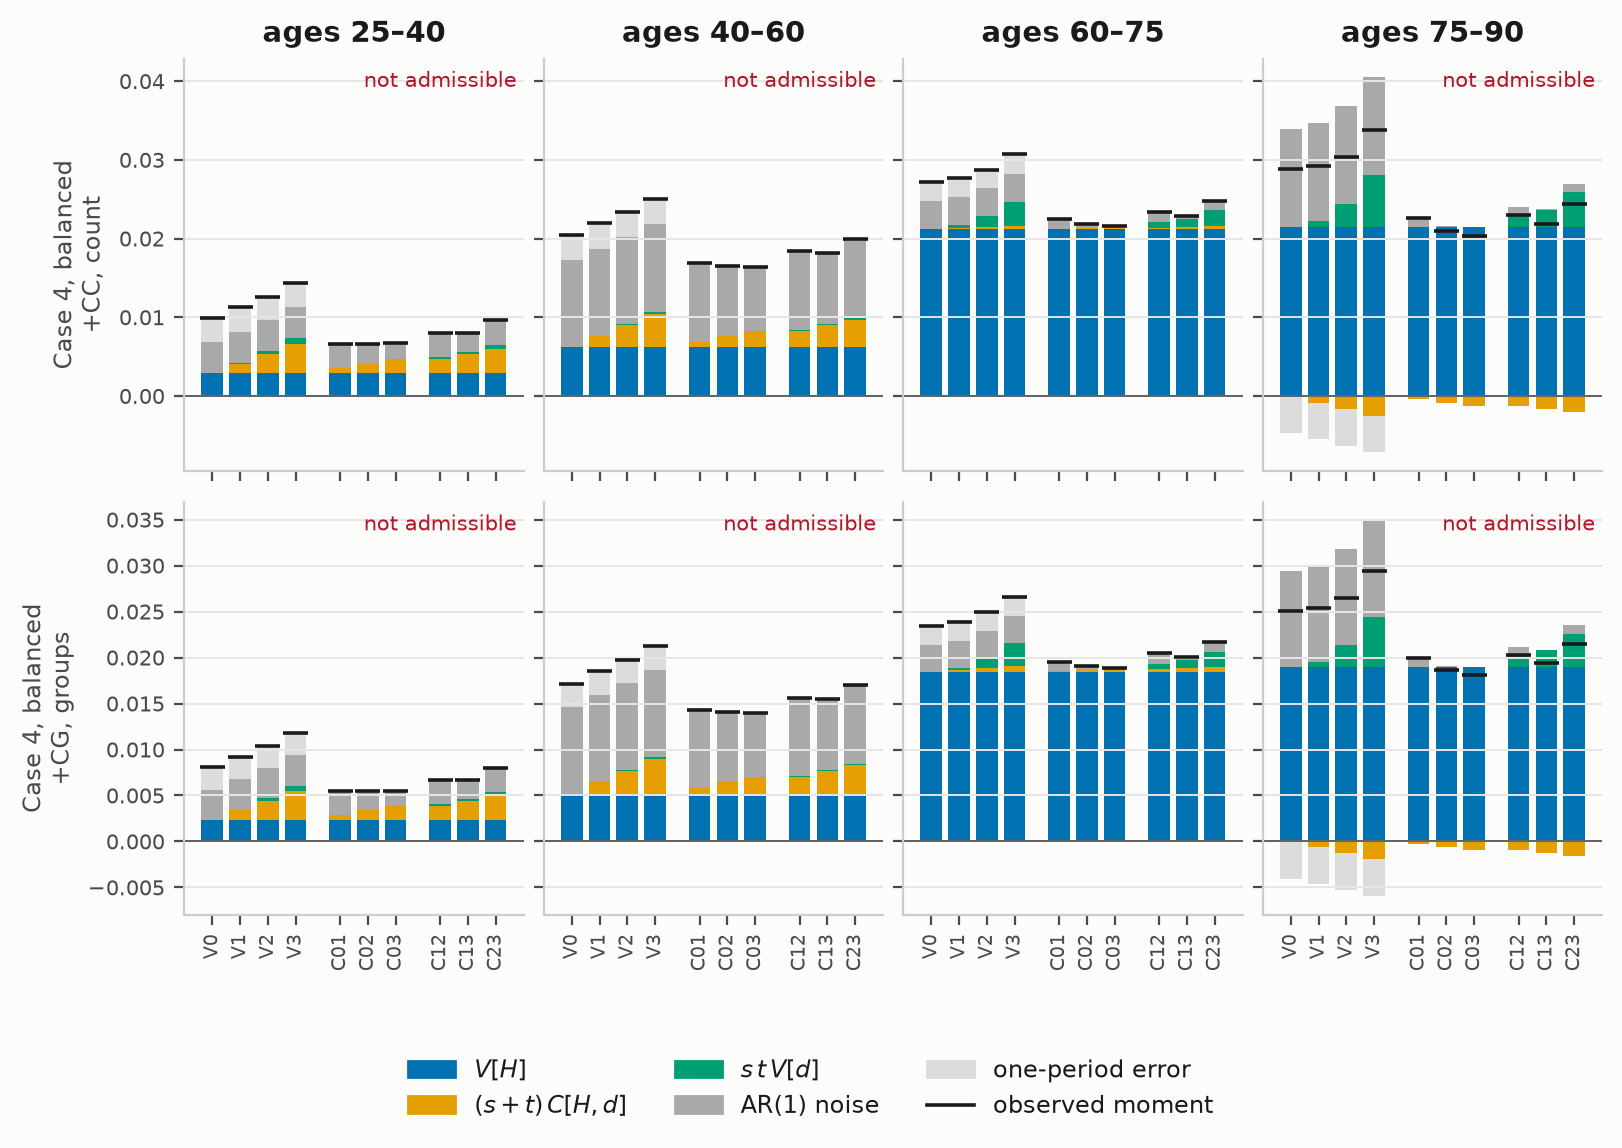
\includegraphics[width=\linewidth]{fig_con_bars_case4_plim3o}
\caption{Case 4 barcharts for P-LIM3+O+CC and P-LIM3+O+CG on $h$, as
Figure~\ref{fig:lim_bars4_pfunc}.}
\label{fig:con_bars4_plim3o}
\end{figure}

\begin{figure}[H]
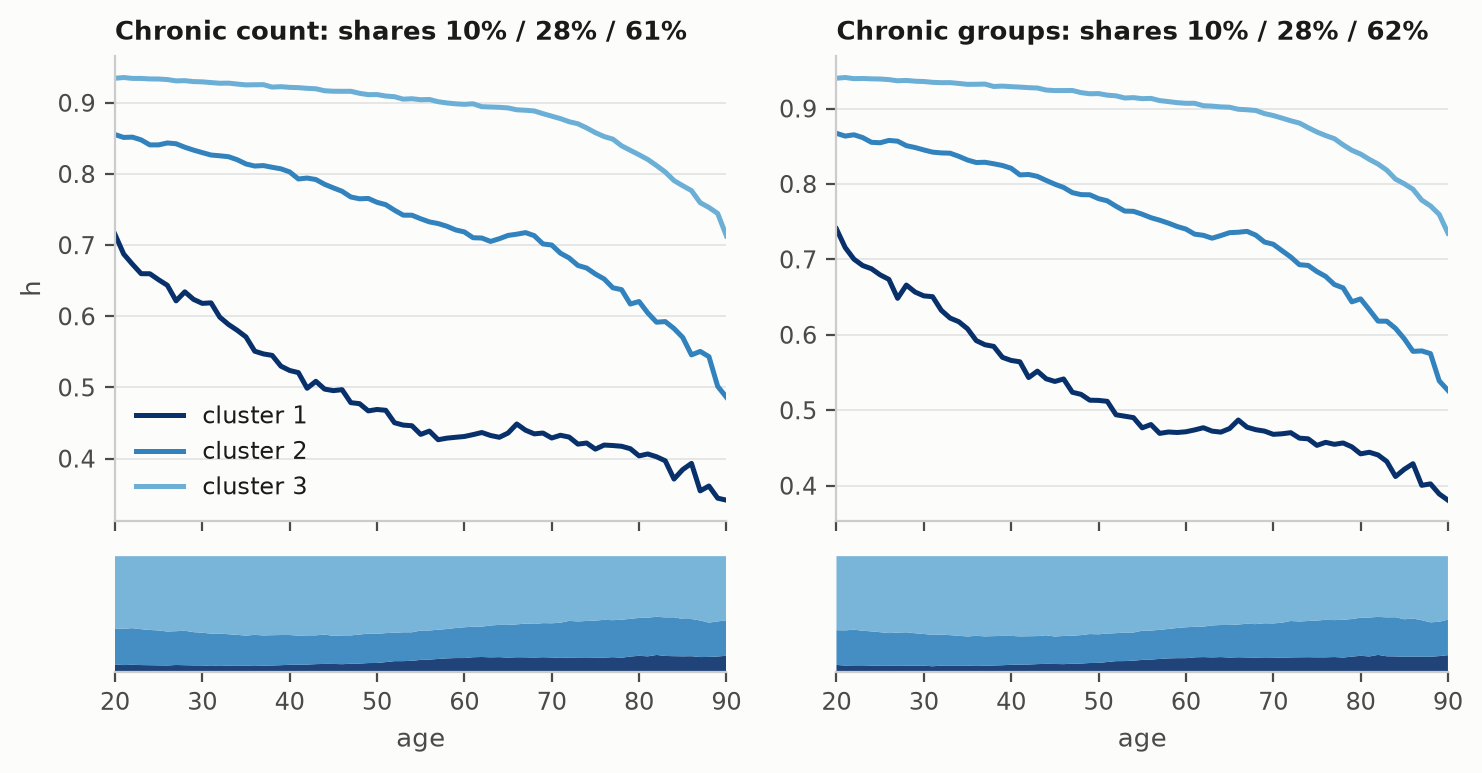
\includegraphics[width=\linewidth]{fig_con_clusters_plim3o}
\caption{Partial K-means, $K=3$, for P-LIM3+O+CC (left) and P-LIM3+O+CG (right) on $h$,
as Figure~\ref{fig:lim_cl_pfunc}.}
\label{fig:con_cl_plim3o}
\end{figure}

\subsection{What this suggests}
\begin{itemize}\itemsep2pt
\item One condition count, added to any limitation bank, gives the pairwise
Case 2 sign path on $h$, flattens the variance into the band, and leaves
convexity where it was. Part of the pairwise improvement is the sample itself;
the count completes it.
\item The six groups carry two to three times the count's weight and do less
for identification, and they take a little off convexity. On this evidence the count is the better way to add
conditions.
\item Either way the price is the panel: every condition bank keeps only 5\%
of the wave-2 entrants' person-years, and those are the longest panels the
covariance surface has.
\end{itemize}

\section{Recommendations}

\begin{enumerate}\itemsep2pt
\item Physical health for lifecycle dynamics: \textbf{P-FUNC} (or the
original GRM). Mental health: \textbf{MENT}. Report both; their correlation
(0.457) is a finding, not an assumption.
\item \textbf{P-FULL} as the descriptive companion when condition burden
should show in the score; P-REC/P-TIMED quantify its recency sensitivity. It
is also the cleaner instrument: on identical people its measurement error is
$.418$ against P-FUNC's $.445$ (\S\ref{sec:meas}). Prefer it for dynamics where
losing the BHPS entrants is acceptable; P-FUNC keeps them at the cost of more
noise.
\item Conditions in the Bayesian mixture as separate channels; ``ever'' is
the right state variable there.
\item Avoid the combined score unless a single index is externally required;
if it is, build the bifactor version first.
\item SF-6D: treat as a mixed physical--mental utility (its closest GRM
cousin is the combined bank), never as a physical measure; licence before
publishing utilities.
\item Report $\theta$ and \code{grmh} together when consequences matter:
$\theta$ is the latent-normal unit the models want, \code{grmh} the
near-linear-in-utilisation unit (\S\ref{sec:convexity}); the choice of
cardinalisation is substantive, not cosmetic.
\item \textbf{Estimate persistence with the state-space specification, not
AR(1).} AR(1) reads the transient noise in a GRM score as fast mean reversion
and attenuates persistence badly --- on the same P-FULL sample, classes 2 and
3 fall from $.90$ and $.86$ to $.27$ and $.39$ --- and between a quarter and
a half of the year-to-year movement in these scores is measurement
(\S\ref{sec:meas}). The state-space model also forecasts better once both
models condition on a person's history, though modestly: $0.084$ nats per
person (\S\ref{sec:ar1}).
\item \textbf{Keep K=3.} A fourth class is reproducible across measures and
the model can recover one in simulation, but it sits at the measurement
ceiling and its defining dynamics are the ones a ceiling produces
(\S\ref{sec:k4}).
\item \textbf{Move the multidimensional ordering constraint onto the chronic
channel} before relying on the state-space multidimensional fits; on the
physical channel it traps chains in an inferior mode (\S\ref{sec:multimort}).
Include mortality to describe survival by class --- the worst class's odds of
dying at 55 are about seven times the healthiest's --- but not to sharpen the
typology, which it leaves unchanged.
\end{enumerate}

\section{Reproducibility}

\begin{center}\small
\begin{tabular}{@{}>{\raggedright\arraybackslash}p{6.1cm}>{\raggedright\arraybackslash}p{8.0cm}@{}}
\toprule
\code{data\_cleaning/03\_build\_measures.py} & SF-12/SF-6D layer; validates
against the construction note (max err 0.0054, 528{,}485 rows, the 6.6-pt
artifact, tariff checks) \\
\code{data\_cleaning/04\_build\_grm.py} & original GRM replicated to
$10^{-5}$ on all 498{,}424 person-waves \\
\code{data\_cleaning/05\_build\_chronic.py} & chronic layer; 100\% timing
coverage; $\ge$ EIT count on 100.000\% of rows \\
\code{data\_cleaning/06\_build\_grm2.py} & all GRM-2 specs; Q3, EAP
identity, invariance, recency weights \\
\code{descriptives/01--20} & measure panel, correlations, every figure, the
ceiling/floor, convexity, class-composition, outcome-prediction and
cost-validation tables \\
\code{clustering/run\_fit.py}, \code{runs/overnight\_queue.py} & the
\S\ref{sec:ar1} batch: generic registry fits, last-two-observations holdout,
per-person held-out densities \\
\code{clustering/run\_multidim.py}, \code{runs/multidim\_queue.py},
\code{multidim\_channel\_decomp.py} & the \S\ref{sec:multifit} batch and its
per-channel held-out decomposition \\
\code{data\_cleaning/}: \code{09\_build\_cost\_proxy.py};
\code{descriptives/}: \code{15\_cost\_validation.py} & the cost proxy of
\code{cost\_proxy\_plan.pdf}, stages 1--3: flat-rate and condition-weighted
indices, and validation against published age, concentration and level
profiles \\
\code{descriptives/16\_cost\_convexity.py},
\code{17\_cost\_age\_interaction.py} & \S\ref{sec:costproxy}: convexity with
pounds on the vertical axis, the twelve-variant costing sensitivity, and the
age interaction with person-clustered standard errors \\
\code{descriptives/19\_k4\_state\_space.py} & \S\ref{sec:k4}: K=3 against
K=4 under the state-space specification --- class trajectories and
composition, the person-by-person class correspondence, persistence and
signal share by class level, in-sample fit and classification certainty \\
\code{clustering/validation/}: \code{synthetic\_recovery\_ssm.py},
\code{synthetic\_recovery\_ssm\_k4.py}, \code{ssm\_holdout\_check.py} &
recovery checks for the state-space specification at K=3 and K=4, and the
validation of its held-out generated quantities against an offline filter \\
\code{clustering/runs/ssm\_queue.py}, \code{ssm\_holdout\_queue.py},
\code{k4\_queue.py}, \code{multidim\_ssm\_queue.py} & the state-space,
holdout-and-control, K=4 and multidimensional state-space batches \\
\code{clustering/holdout\_matched.py} & \S\ref{sec:ar1}'s matched held-out
comparison: AR(1) and AR(1) plus measurement error scored offline on the same
people, rows, draws and estimands \\
\code{data\_cleaning/}: \code{07\_build\_limitation\_}
\code{banks.py}; \code{measures/gpcm.py}; \code{tests/test\_gpcm.py} & \S\ref{sec:limbanks}: the six
limitation banks under the graded-response and partial credit models; $Q_3$,
EAP identity, the weighted-sum check, and P-FUNC reproduced exactly;
\S\ref{sec:conbanks}: the ten condition banks, and P-FULL reproduced exactly \\
\code{descriptives/}: \code{baseline\_measures/}, scripts 01--11 & the baseline criteria workbook
and \S\ref{sec:limbanks}'s criteria, weights, identification moments,
clusters, figures and tables; scripts 01--06 reproduce the first version of
the workbook exactly \\
\code{descriptives/}: \code{18\_roster\_difference.py},
\code{20\_multidim\_mortality.py} & the P-FULL/P-FUNC roster diagnostic; the
multidimensional state-space and mortality fits on their better-mode chains \\
\bottomrule
\end{tabular}
\end{center}

Everything under \code{data/} derives from licensed UKHLS microdata and is
never committed; all figures are aggregate statistics.

\subsection*{References}
{\small
Barnett et al.\ (2012) \emph{Lancet} 380:37--43.
Bauer \& Hussong (2009) \emph{Psychol Methods} 14:101--25.
Cella et al.\ (2010) \emph{J Clin Epidemiol} 63:1179--94.
Farivar, Cunningham \& Hays (2007) \emph{Health Qual Life Outcomes} 5:54.
Goldberg et al.\ (1997) \emph{Psychol Med} 27:191--7.
Graetz (1991) \emph{Soc Psychiatry Psychiatr Epidemiol} 26:132--8.
Hankins (2008) \emph{Clin Pract Epidemiol Ment Health} 4:10.
Johnston, Propper \& Shields (2009) \emph{J Health Econ} 28:540--52.
Jones (2010) \emph{Models for health care}, HEDG WP 10/01.
Katz et al.\ (1963) \emph{JAMA} 185:914--9.
Kelly et al.\ (2024) \emph{Pharmacoepidemiol Drug Saf} 33:e5701.
Manning \& Mullahy (2001) \emph{J Health Econ} 20:461--94.
Kriegsman et al.\ (1996) \emph{J Clin Epidemiol} 49:1407--17.
Mitnitski, Mogilner \& Rockwood (2001) \emph{ScientificWorldJournal} 1:323--36.
Muraki (1992) \emph{Appl Psychol Meas} 16:159--76.
Preen et al.\ (2006) \emph{J Clin Epidemiol} 59:940--6.
Samejima (1969) \emph{Psychometrika Monogr} 17.
Searle et al.\ (2008) \emph{BMC Geriatr} 8:24.
Sylvestre \& Abrahamowicz (2009) \emph{Stat Med} 28:3437--53.
Verbrugge \& Jette (1994) \emph{Soc Sci Med} 38:1--14.
Wainer \& Kiely (1987) \emph{J Educ Meas} 24:185--201.
Ware, Kosinski \& Keller (1996) \emph{Med Care} 34:220--33.
Yen (1993) \emph{J Educ Meas} 30:187--213.
Rose (1981) \emph{BMJ} 282:1847--51; (1985) \emph{Int J Epidemiol} 14:32--8.
Zweifel, Felder \& Meiers (1999) \emph{Health Econ} 8:485--96.
}

\end{document}
